\documentclass[a4paper, 11pt]{book}
\usepackage{microtype}
\usepackage{mathtools}
\usepackage{amssymb}
\usepackage{amsfonts}
\usepackage{amsthm}
\usepackage{fontspec}
\usepackage{lmodern}
\usepackage[]{graphicx}
\usepackage{physics}
\usepackage{chemfig}
\usepackage{tikz}
\usepackage{tikz-feynman}
\usepackage{tikzorbital}
\usepackage{dsfont}
\usepackage[]{geometry}
\usepackage{xcolor}
\usepackage{fancyref}
\usepackage{fancyhdr}
\usepackage{float}
\usepackage[]{tipa}
\usepackage{slashed}
\usepackage{titlesec}
\usepackage{subfiles}
\usepackage[style=alphabetic]{biblatex}
\usepackage[colorlinks=true,linkcolor=black,urlcolor=blue,citecolor=red]{hyperref}
\addbibresource{/home/birrabenzina/Dropbox/appunti/bibliografia/bib.bib}
\usepackage{fancyhdr}
\definecolor{titlepagecolor}{cmyk}{1,.60,0,.40}
\newcommand{\plogo}{\fbox{$\mathcal{MC}$}}
\setlength{\headheight}{13.6pt}
\fancyhf{}
\fancyhead[R]{\textbf{\textsf{\thepage}}}
\fancyhead[LE]{\textbf{\textsf{\leftmark}}}
\fancyhead[LO]{\textbf{\textsf{\rightmark}}}
\pagestyle{fancy}
\titleformat{\chapter}[block]%
{\bfseries\large}%
{\fontsize{40}{30}\selectfont\color{gray}\textsf\thechapter}%
{1.5em}
{\fontsize{25}{20}\selectfont\scshape}%
[\vspace{-1ex}%
	\hfill%
\rule{\textwidth}{0.5pt}]
\renewcommand{\maketitle}[5][7.5cm]{
	\begin{titlepage}
		\newgeometry{left=#1}
		\scshape
		\pagecolor{titlepagecolor}
		%		\noindent
		%		\includegraphics[width=2cm]{sfondo}\\[-1em]
		%		\vskip\baselineskip
		\noindent
		\color{white}
		{\Huge #2}
		\vskip0.1\baselineskip\noindent
		\makebox[0pt][l]{\rule{1.2\textwidth}{0.5pt}}
		\par
		\noindent
		\textit{Università degli Studi di Roma "La Sapienza"}\\\textit{Physics BSc}
		\vskip\baselineskip
		\vskip\baselineskip
		\noindent
		\textsf{#5}
		\vfill
		\noindent
		\textsf{Notes on #2}
		\vskip0.1\baselineskip\noindent
		\makebox[0pt][l]{\rule{1.2\textwidth}{0.5pt}}
		\vskip\baselineskip
		\noindent
		\textsf{#3}
		\vskip\baselineskip
		\noindent
		\textsf{\Large Version #4}
		\restoregeometry
		\pagecolor{white}
	\end{titlepage}
	\begin{titlepage}
		\centering
		\scshape
		\rule{\textwidth}{1.6pt}\vspace*{-\baselineskip}\vspace*{2pt}
		\rule{\textwidth}{0.4pt}

		\vspace{0.75\baselineskip}
		{\Huge #2\\}
		\vspace{0.75\baselineskip}
		\rule{\textwidth}{0.4pt}\vspace*{-\baselineskip}\vspace{3.2pt}
		\rule{\textwidth}{1.6pt}
		\vspace{2\baselineskip}

		Notes on #2

		\vspace*{6.5\baselineskip}

		Written by

		\vspace{0.5\baselineskip}

		{\scshape\Large  #5}
		\vspace{0.5\baselineskip}

		\textit{Università degli Studi di Roma "La Sapienza"\\ Physics BSc}

		\vfill

		\plogo

		\vspace{0.7\baselineskip}

		#3

		\vspace{0.5\baselineskip}

		{\Large Version #4}
		\newpage
	\end{titlepage}
}
\renewcommand{\vec}[1]{\mathbf{#1}}
\renewcommand{\trace}{\mathrm{Tr}}
\newcommand{\ver}[1]{\vec{e}_{#1}}
\newcommand{\1}{\opr{\mathds{1}}}
\newcommand{\lbar}{\mbox{\textipa\textcrlambda}}
\newcommand{\unit}[1]{\ \mathrm{#1}}
\newcommand{\diff}[2][]{\ \mathrm{d}^{#1}#2}
\newcommand{\ddiff}[3][]{\ \mathrm{d}^{#1}#2\mathrm{d}^{#1}#3}
\newcommand{\dddiff}[4][]{\ \mathrm{d}^{#1}#2\mathrm{d}^{#1}#3\mathrm{d}^{#1}#4}
\newcommand{\ham}{\mathcal{H}}
\newcommand{\opr}[1]{\hat{#1}}
\newcommand{\adj}[2][]{#2^{\dagger#1}}
\newcommand{\tposed}[1]{#1^{\text{T}}}
\newcommand{\pcomm}[2]{\comm{#1}{#2}_{PB}}
\newcommand{\U}{\opr{\mathcal{U}}}
\newcommand{\N}{\mathbb{N}}
\newcommand{\cc}[1]{\overline{#1}}
\newcommand{\lc}[1]{\epsilon_{#1}}
\newcommand{\kd}[1]{\delta_{#1}}
\newcommand{\kdopr}[1]{\opr{\delta}_{#1}}
\newcommand{\mc}[1]{\mathcal{#1}}
\newcommand{\ladopru}[1]{\opr{#1}_{+}}
\newcommand{\ladoprd}[1]{\opr{#1}_{-}}
\newcommand{\ladoprpm}[1]{\opr{#1}_{\pm}}
\newcommand{\vecopr}[1]{\opr{\vec{#1}}}
\newcommand{\up}{\uparrow}
\newcommand{\down}{\downarrow}
\newcommand{\hilbert}{\mathbb{H}}
\newcommand{\sph}{Y^{m_l}_l(\theta,\phi)}
\newcommand{\tsph}{\mc{Y}^{ls}_{jm}(\theta,\phi)}
\newcommand{\oham}{\opr{\mathcal{H}}}
\newcommand{\sla}[1]{\slashed{#1}}
\newcommand{\term}[3][]{^{#3}#2_{#1}}
\newcommand{\F}{\hat{\mathcal{F}}}
\newcommand{\R}{\mathbb{R}}
\newcommand{\C}{\mathbb{C}}
\newcommand{\dopr}{\hat{\rho}}
\newcommand{\qsum}{\sideset{}{'}\sum}
\newtheorem{pos}{Postulate}
\newtheorem{thm}{Theorem}
\theoremstyle{plain}
\newtheorem{defn}{Definition}
\newtheorem{cor}{Corollary}
\newtheorem{hyp}{Hypothesis}
\begin{document}
\maketitle{Quantum Mechanics}{\today}{$0.7\beta$}{Matteo Cheri}
\tableofcontents
	\part{Quantum Mechanics}
	\chapter{The Failure of Classical Physics}
	The failure of classical physics starts in the first years of the 1900s, when the first experimental measurements on the world of the very small begun. The first discrepancies found, after Planck's quantization of energy ``trick'' for avoiding the UV catastrophe, were in the experimental results given from the measurements of the wavelength of the emission of Hydrogen, Bremsstrahlung radiation and the famous photoelectric effect.\\
	The first approaches for a correct theoretical modelization of a Hydrogen atom were put forward by Thomson, where the atom itself is considered as a charged sphere, in which there are inside positive and negative charges.\\
	For Hydrogen we will have a sphere of radius $a$ with charge $\abs{q}=e=1.6\cdot10^{-19}\unit{C}$. Using Gauss' theorem, we know that the flux of the electric field $\vec{E}$ will be given by the following piecewise function
	\begin{subequations}
	\begin{equation}
		\Phi_E(r)=\begin{dcases}
			4\pi e\frac{r^3}{a^3}&0\le r\le a\\
			4\pi e& r\ge a
		\end{dcases}
		\label{eq:thomsoneflux}
	\end{equation}
	Since we are in a spherically simmetrical system, the flux of the $\vec{E}$ field will simply be $4\pi r^2\vec{E}(r)$, and our $\vec{E}$ field will be
	\begin{equation}
		\vec{E}(r)=\begin{dcases}
			\frac{er}{a}\ver{r}&0\le r\le a\\
			\frac{e}{r^2}\ver{r}&r\le a
		\end{dcases}
		\label{eq:thomsonefield}
	\end{equation}
\end{subequations}
	Since $\vec{E}$ is conservative, we can define a scalar potential $\phi$ such that $\nabla\phi=\vec{E}$. This function is easily determined by the solution of a 1st order ODE
	\begin{subequations}
	\begin{equation}
		\left\{\begin{aligned}
			&\derivative{\phi}{r}=\begin{dcases}
				-\frac{er}{a^3}&0\le r\le a\\
				-\frac{e}{r^2}&r\ge a
			\end{dcases}\\
			&\lim_{r\to\infty}(\phi(r))=0
		\end{aligned}\right.
		\label{eq:thomsonscalarpot}
	\end{equation}
	The ODE is a separable differential equation with the following solution
	\begin{equation}
		\phi(r)=\begin{dcases}
			\frac{3e}{2a}-\frac{er^2}{2a^3}&0\le r\le a\\
			-\frac{e^2}{r}&r\ge a
		\end{dcases}
		\label{eq:thomsonscalarpotential}
	\end{equation}
\end{subequations}
	Since the total charge of the system is $q=-e$, and the potential energy of the system will be given from the scalar potential times the total charge, we have that $V(r)=-e\phi(r)$.\\
	Since the ionization energy is defined as $E_I=V(0)$, we get for Hydrogen,
	\begin{equation*}
		E_I=-\frac{3e^2}{2a}\approx-13.6\unit{eV}
	\end{equation*}
	For evaluating the emission frequency of this system, we write the Hamiltonian for a harmonic oscillator with the mass of an electron, $m_e$, coupled to a Hamiltonian with the potential $V(r)$.\\
	The Hamiltonian will then be defined piecewise as such
	\begin{equation}
		\ham(p,r)=\begin{dcases}
			\frac{p^2}{2m_e}+\frac{1}{2}m_e\omega^2r^2\\
			\frac{p^2}{2m_e}+\frac{e^2r^2}{2a^3}
		\end{dcases}
		\label{eq:thomsonham}
	\end{equation}
	Solving the system for $\omega$ we get
	\begin{equation*}
		\omega=\sqrt{\frac{e^2}{m_ea^3}}
	\end{equation*}
	Plugging the measured values of the electron mass and the radius of the charged sphere, we get a frequency $\nu\approx1.2\cdot10^{15}\unit{Hz}$ and a corresponding wavelength of $\lambda\approx3\cdot10^3\unit{\AA}$.\\
	Although the values obtained from this classical model of the atom core are consistent, the whole idea has been disproven by Geiger and Madsen, whom have demonstrated that if a Gold sheet is irradiated with $\alpha$ particles, most of them will pass through without scattering, some get sligthly deflected after interacting with the Gold atoms and another part gets deflected with angles that are completely incompatible with Thomson's model.\\
	A different model which explains the Geiger-Madsen experiment is the Rutherford model of the atom, where the system is evaluated as two opposed charges, the nucleus positively charged, and the orbiting electrons with negative charge.\\
	The total energy of the Rutherford atom can be calculated using the classical Virial theorem, which gives
	\begin{equation}
		E=\frac{1}{2}m_ev^2-\frac{e^2}{a}=-\frac{e^2}{2a}
		\label{eq:rutherfordenergy}
	\end{equation}
	Forcing in the measured valued for $E_I$, we get for Hydrogen $a\approx0.5\unit{\AA}$ and $\lambda\approx455\unit{\AA}$.\\
	Although these values are consistent with observations, the model isn't physically accurate, since the electrons in these orbits have a nonzero acceleration, which brings them to emit sincrotron radiation and consequently lose angular momentum, falling towards the nucleus.\\
	If one explicits all the values in game with such system, will get that a random atom will have a mean life of $10^{-8}\unit{s}$, which is completely in contrast with observation, since atoms exist, and didn't get annihilated $10^{-8}\unit{s}$ after their formation in the early universe.\\
	The final blow to this huge crisis in classical physics has been given by Einstein and his discovery of the photoelectric effect, where it's shown that, if a metal is irradiated from a source with an energy $E>W$, with $W$ a work function, there is an emission of electrons linearly proportional to the frequency of the radiation, with coupling constant being exactly Planck's constant, $h=6.6\cdot10^{-34}\unit{Js}$. The inverted experiment gives instead a ``stopping radiation'', Bremsstrahlung in German, where at given frequencies the blackbody radiation of the source gets ``stopped''. This kind of behavior is not explainable with classical physics, which gave rise to the formulation of quantum mechanics.\\
	The photoelectric effect, with its astonishing results, gave rise to the idea that radiation is quantized, hence it behaves as a particle, and at the same time, due to the certainity behind classical optics, it has the behavior of a wave.
	\section{Old Quantum Mechanics}
	After the discovery of Bremsstrahlung and the photoelectric effect, there has been an attempt to formalize this new mechanics of quanta by Bohr, through 3 hypotheses
	\begin{hyp}[Bound States]
		For any atom, only states with discrete energies $E_n$ are allowed, where $E_n$ is a monotonically increasing succession of values, called Energy Levels. The set of these discrete states is called the set of Bound States, the minimum value of this succession is $E_0$ and is commonly referred to as Ground State.
	\end{hyp}
	\begin{hyp}[Transition Between Levels]
		When the system is in a bound state radiates only in transitions between levels.\\
		Taking a level $E_n$ and a level $E_m$ where $m>n$, the frequency of the radiation is
		\begin{equation*}
			\nu_{nm}=\frac{\abs{E_m-E_n}}{h}
		\end{equation*}
		Where $h$ is Planck's Constant.
	\end{hyp}
	\begin{cor}[Ritz Combination Principle]
		The emission spectrum of an atom, with this hypothesis, is then given by evaluating all the energy differences of the absorption spectrum's difference, hence
		\begin{equation*}
			\abs{\nu_{0n}-\nu_{0m}}=\abs{\frac{E_n-E_0}{h}-\frac{E_m-E_0}{h}}=\frac{\abs{E_n-E_m}}{h}=\nu_{nm}
		\end{equation*}
	\end{cor}
	\begin{hyp}[Bohr-Sommerfield Quantization]
		Defining $\hbar$ as $h/2\pi$ as the reduced Planck Constant, we get that the only permitted orbits are those where $L\propto n\hbar$.\\
		For an orbit $\gamma$ then holds that
		\begin{equation*}
			L=\oint_{\gamma}p\diff{q}=n\hbar
		\end{equation*}
		For a circular orbit, $L=\mu vr$, hence
		$\mu vr=n\hbar$
	\end{hyp}
	For an Hydrogen atom we then get the following results.\\
	Considering that the system is virialized, we can write the energy as such
	\begin{subequations}
		\begin{equation}
			E=\frac{1}{2}V=-\frac{Ze^2}{2r}
			\label{eq:bohrenergy}
		\end{equation}
		The third Bohr hypothesis requires that $\mu vr=n\hbar$, with $\mu$ being the reduced mass of the system nucleus-electron.\\
		Squaring the previous relation and inserting it in the expression of energy, we get
		\begin{equation}
			\frac{1}{2}\mu v^2=\frac{n^2\hbar^2}{2\mu r^2}=\frac{Ze^2}{2r}
		\end{equation}
		From this we get that the only possible orbits are at a radius $r_n$, where
		\begin{equation*}
			r_n=\frac{n^2\hbar^2}{\mu Ze^2}=\frac{n^2m_ea_B}{Z\mu}
		\end{equation*}
		With $a_B=\hbar^2/m_ee^2$ a constant with dimensions of length, called Bohr radius.\\
		Inserting what we have just derived in \eqref{eq:bohrenergy} we get the succession of quantized levels of energy, with the following relation
		\begin{equation}
			E_n=-\frac{Z^2e^2m_e}{2a_Bn^2}
			\label{eq:atomicbohrenergy}
		\end{equation}
	\end{subequations}
	Inserting $Z=1$ for restricting these levels to hydrogen, we get, with the approximation $\mu\approx m_e$ that
	\begin{equation}
		\begin{aligned}
			r_n&=n^2a_B\\
			a_B&=\frac{\hbar^2}{m_ee^2}=0.53\unit{\AA}\\
			E_n&=-\frac{e^2}{2a_Bn^2}
		\end{aligned}
		\label{eq:bohrhydrogenresult}
	\end{equation}
	The values obtained are in accord with experimental results, but the new ``theory'' of quantum mechanics had yet to be formalized with a set of fundamental principles.
	\section{Wave-Particle Duality}
	The photoelectric effect, as said before, gave rise to the discovery of the particle-like behavior of light. L. de Broglie, put forward the following problem:\\
	Taking as true the wave like behavior of the electromagnetic radiation, and at the same time taking as true the particle behavior of the same, there must be a particular wavelength for any particle, for which can be then defined a \textit{matter wave}, which has the same ondulatory behavior of classical waves, while still having all the properties of matter.\\
	Taking as an Ansatz the Bohr-Sommerfield quantization hypothesis, we get that
	\begin{equation*}
		pL=nh
	\end{equation*}
	Dividing by $p$ we finally get that
	\begin{equation*}
		L=n\frac{h}{p}
	\end{equation*}
	Since for a photon $\lambda=h/p$, we get the following hypothesis
	\begin{hyp}[de Broglie Hypothesis]
		A wave is associated with each particle, and its wavelength is given by the relation $\lambda=h/p$. All the allowed orbits are those which contain an integer number of wavelengths.
	\end{hyp}
	We can then define the \textit{de Broglie wavelength} of matter as such:\\
	Since $p=\sqrt{2mE}$, we get
	\begin{equation}
		\lambda_{DB}=\frac{h}{\sqrt{2mE}}
		\label{eq:debrogliewavelength}
	\end{equation}
	If preferred, defining a ``reduced'' de Broglie wavelenght as $\lbar=\lambda_{DB}/2\pi$, we get, in terms of $\hbar$
	\begin{equation*}
		\lbar=\frac{\hbar}{\sqrt{2mE}}
	\end{equation*}
	\section{Experimental Verifications of Quantum Mechanics}
	\subsection{Double Slit Experiment and Quantum Measurement}
	In order to verify de Broglie's hypothesis of matter waves, many experiments were carried on, but the one that is really worth of notice is the \textit{double slit experiment}.\\
	Let a beam of monochromatic light hit a completely opaque screen, on which there are two parallel slits. Due to the wave nature of electromagnetic radiation, the light passing through the two waves interferes with itself, and if a detector is put on front of such screen, a diffraction pattern can be observed and measured, as expected from classical electromagnetism and optics. In terms of photons, this diffraction pattern indicates where more photons hit the detector and where less did, and the diffraction can be seen as mere interaction with photons that got through different slits.\\
	The real hassle comes when the same experiment is repeated without a continuous beam of light, but with a single photon. In this case an interference pattern \emph{can't} be explained with interacting photons, as there is a single photon in the whole system.\\
	According to the corpuscular model, the photon must pass through one single slit, but the interference pattern wouldn't be observed in this case, giving a further confirmation of the wave-particle duality.\\
	Getting back again to the first case, we can also try to interpret the interference pattern as a sum of the interference patterns of the photons passing only through one of the two slits. Introducing the idea of \textit{state}, we can identify with $\ket{A},\ket{B}$ the diffraction patterns of the photons passing through a single slit, and with $\ket{C}$ the interference pattern identified in the doble slit experiment.\\
	It's easy to see that the final state isn't exactly a sum of the first two.\\
	Leaving the world of classical physics, we can interpret the final state $\ket{C}$ as being a ``mixture'' of the state $\ket{A}$ and $\ket{B}$. taking $a,b$ constants, then we can write that
	\begin{equation*}
		\ket{C}=a\ket{A}+b\ket{B}
	\end{equation*}
	This result has no similar results in classical physics, since, if evaluated for a single photon, it explicitly indicates that the photon is passing through both slits at the same time!\\
	A similar experiment uses a Mach-Zehnder interferometer, where a beam of neutrons gets shot through two different paths, where at the end of both a detector is carefully placed.\\
	The result for a single neutron experiment are basically the same of the double slit experiment, because it is measured that the single neutron passes through both paths, and gets then measured from both detectors.\\
	Modifying the experiment, and putting a detector on both slits, removes this indecision on which slit the particle went through (or path in the interferometer), and would let a detailed description of the construction of the interference pattern to be brought up from data.\\
	What is observed though is extremely different from what is expected, in fact, measuring from which slit the particle goes through completely destroys the interference pattern, and what is measured is a corpuscular behavior of the particles.\\
	This result, tells us that measuring a state, changes it. In fact, it changes the state in such a way that we can either have an interference pattern of a wave-like behavior or a particle-like behavior.\\
	In fact, wave-particle duality still holds, but now gets a whole different meaning: \textit{particles aren't waves nor corpuscules, but both at the same time}. This affirmation has no meaning whatsoever in the classical world that we perceive, and it's the key factor in making quantum mechanics not understandable with physical intuition.\\
	Although not humanly understandable, quantum mechanics can be formalized in a full fledged physical theory with a formal mathematical background, which lets us ``understand'' quantum mechanics through mathematics. In fact, we can grasp the mathematics of it, even without grasping the physical reality behind it.
	\chapter{The Fundamentals}
	\section{Dirac Notation}
	In order to fully grasp this and the future chapters is useful to really know how Dirac notation works in a mathematical framework. In Dirac notation, a vector of a complex Hilbert space $\mathbb{H}$ is indicated with the following notation: $\ket{\cdot}$, called a \textit{ket}, where in place of the dot there is usually a label or an index. Hence, if we have a vector $\vec{a}\in\mathbb{H}$, this vector can be indicated as $\ket{a}\in\mathbb{H}$. Defining the dual space of $\mathbb{H}$ as the space of all linear functionals, i.e. all elements $\vec{b}\in\mathbb{H^{\star}}$ such that $\vec{b}\cdot\vec{a}=\lambda\in\mathbb{C}$, we define such vectors (or covectors) with the notation $\bra{b}$, called \textit{bra}. With this notation, the scalar product simply becomes $\bra{b}\ket{a}=\lambda$. It's also useful to remember that there exist an isomophism $\iota:\mathbb{H}\to\mathbb{H^{\star}}$, where it is defined as follows
	\begin{equation*}
		\iota(\vec{a})=\overline{\vec{a}}^{\text{T}}=\overline{\vec{a}^{\text{T}}}\in\mathbb{H^{\star}}\quad\forall\vec{a}\in\mathbb{H}
	\end{equation*}
	In Dirac notation, we will then have the following
	\begin{equation*}
		\iota(\ket{a})=\overline{\ket{a}}^{\text{T}}=\overline{\ket{a}^{\text{T}}}=\bra{a}\quad\forall\ket{a}\in\mathbb{H}
	\end{equation*}
	\subsection{Generalized Vectors and Tensors in Dirac Notation}
	Generalizing to tensor spaces, we get the following notation equivalences in the case of rank 2 tensors.\\
	Let $T_{ij},G_{i}^{j},H^{ij}$ be tensors in the spaces, respectively $\mathbb{H}^{\star}\otimes\mathbb{H}^{\star},\mathbb{H}^{\star}\otimes\mathbb{H},\mathbb{H}\otimes\mathbb{H}$\\
	In Dirac notation, since they represent the direct product of two vectors (or covectors), they can be indicated as such
	\begin{equation}
		\begin{aligned}
			T_{ij}&\longrightarrow\bra{i}\otimes\bra{j}=\bra{i}\bra{j}=\bra{ij}\\
			G^i_j&\longrightarrow\ket{i}\otimes\bra{j}=\ket{i}\bra{j}\\
			H^{ij}&\longrightarrow\ket{i}\otimes\ket{j}=\ket{i}\ket{j}=\ket{ij}
		\end{aligned}
		\label{eq:tensorsdiracnot}
	\end{equation}
	Remembering that the isomorphism between the space and its dual is given by a trasposition and a complex conjugation, we have that the operation of index raising and index lowering (also known as musical isomorphisms), in Dirac notation will be indicated as follows:
	\begin{equation}
		T^{ij}=\overline{T_{ij}^{\text{T}}}=\overline{T_{ji}}\longrightarrow\ket{i}\ket{j}=\bra{j}\bra{i}
		\label{eq:musicalisomorphism}
	\end{equation}
	This is especially useful when treating the contraction of all indexes of a tensor.\\
	Let $R_{ij}=a_ib_j$ and $S^{ij}=c^id^j$. The product $R_{ij}S^{ij}$ will then be, using the Einstein convention for repeated indexes and the rules defined before for raising and lowering indexes,
	\begin{equation}
		R_{ij}S^{ij}=a_ib_jc^id^j=\overline{b^ja^i}c^id^j\to\bra{b}\bra{a}\ket{c}\ket{d}=\bra{a}\ket{c}\bra{b}\ket{d}
		\label{eq:doublescalarprod}
	\end{equation}
	Since a tensor product of two vector spaces is a vector space itself, it's common to directly use superindexes or labels in the labels of the kets and bras, such that a tensor $\ket{ij}=\ket{I}$, where $I$ is the chosen label. It's not hard to then generalize the notation to rank-$n$ tensors.\\
	There is only one exception, irreducible tensors. Since they can't be factorized as the direct product of two vectors, they're usually directly indicated with a simple label as before.\\
	\subsection{Function Spaces and Linear Operators}
	Since quantum mechanics can be also represented with elements of function spaces, Dirac notation can be extended to indicate even functions and operators.\\
	Let $\mathcal{F}$ be a function space, and let $\psi\in\mathcal{F}$ be an element of such.\\
	We can write the function $\psi(x):\mathbb{C}\to\mathbb{R}$ as the projection of the element of $\mathcal{F}$ to the field of complex numbers $\mathbb{C}$. In Dirac notation this becomes
	\begin{equation}
		\psi(x)\leftrightarrow\bra{x}\ket{\psi}
		\label{eq:functionstokets}
	\end{equation}
	An operator, is a linear endomorphism of $\mathbb{H}$. If we have an operator $\opr{\eta}$ bounded, and an operator $\opr{\sigma}$ unbounded, their definition spaces will be the following
	\begin{equation}
		\begin{aligned}
			\opr{\eta}&:\mathbb{H}\to\mathbb{H}\\
			\opr{\sigma}&:\mathcal{D}\subset\mathbb{H}\to\mathcal{D}\subset{H}
		\end{aligned}
		\label{eq:linopdefi}
	\end{equation}
	Since they're linear, if we define a new operator $\opr{\iota}_i$, where $\opr{\iota}_1=\opr{\eta}$ and $\opr{\iota}_2=\sigma$, we have, that $\forall\alpha,\beta\in\mathbb{C}$ and $\forall\ket{A},\ket{B}\in\mathcal{D}$, ($\in\mathbb{H}$ if we're considering a bounded operator)
	\begin{equation}
		\opr{\iota}_i\left( \alpha\ket{A}+\beta\ket{B} \right)=\alpha\opr{\iota}_i\ket{A}+\beta\opr{\iota}_i\ket{B}
		\label{eq:lineardef}
	\end{equation}
	Let's now define an operator $\opr{R}$ such that $\opr{R}\psi(x)=e^{i\pi}\psi(x)$. In Dirac notation it's simply $\opr{R}\ket{\psi}=e^{i\pi}\ket{\psi}$, nothing changes much.\\
	Although, since operators acting on functions can be seen as tensors (or matrices) acting on vectors, we can write the (infinite) matrix representation of such objects, as such:\\
	Let $\vec{e}_i,\vec{e}_j$ be two basis elements of $\mathcal{F}$. We then will have the following relation, if the scalar product is indicated as $\langle\cdot,\cdot\rangle$
	\begin{equation*}
		R_{ij}=\langle\vec{e}_i,\opr{R}\vec{e}_j\rangle
	\end{equation*}
	In Dirac notation, its formulation it's similar in shape, and it's written as such
	\begin{equation*}
		R_{ij}=\bra{i}\opr{R}\ket{j}
	\end{equation*}
	If now we define the \textit{adjoint} operation (indicated with ($\dagger$) as the composition of complex conjugation and transposition ($\square^{\dagger}=\overline{\square}\circ\square^{\text{T}}$), we have
	\begin{equation*}
		\adj{R_{ij}}=\adj{\langle\vec{e}_i,\opr{R}\vec{e}_j\rangle}=\langle\vec{e}_j\adj{\opr{R}},\vec{e}_i\rangle
	\end{equation*}
	Without writing the equivalent operation in Dirac notation, and just confronting how the adjoint operator works, we get immediately get how it will behave with kets and bras. The operator will act on the right, and its adjoint on the left.\\
	Let $\ket{a}$ be an eigenvector (or eigenket) of $\opr{R}$, with eigenvalue $\alpha$. We then can express the fact that the operator acts on the right, and its adjoint on the left using $\opr{R}$'s secular equation
	\begin{equation*}
		\begin{aligned}
			\opr{R}\ket{a}&=\alpha\ket{a}\\
			\bra{a}\adj{\opr{R}}&=\bra{a}\overline{\alpha}
		\end{aligned}
	\end{equation*}
	But since applying the double adjoint means applying the identity transformation, we get that
	\begin{equation*}
		\adj{\left[\adj{\left( \opr{R}\ket{a} \right)}\right]}=\adj{\left(\bra{a}\adj{\opr{R}}\right)}=\adj{\left(\bra{a}\overline{\alpha}\right)}=\alpha\ket{a}=\opr{R}\ket{a}
	\end{equation*}
	Hence, an adjoint of an operator acts on the left, and the adjoint of the adjoint operator is the operator itself, and if a ket is a solution to the secular equation, its equivalent bra will be the solution to the adjoint secular equation.\\
	Let's remember that in general, $\adj{\opr{R}}\ne\opr{R}$, hence generally $\opr{R}\ket{A}\ne\bra{A}\opr{R}$
	\section{Axioms of Quantum Mechanics}
	The first postulate of quantum mechanics used to formalize mathematically its structure is the \textit{superposition principle}
	\begin{pos}[Superposition Principle]
		The state of a quantum system is a vector of a separable Hilbert space ($\mathbb{H}$), and if two different vectors are proportional to eachother, they represent the same state. This space must be endowed with a Hermitian scalar product and its dimension is usually infinite.
	\end{pos}
	Since this Hilbert space is a linear vector space, it's algebraically closed, which means that, for two different states $\ket{a}$ and $\ket{b}$, with $\alpha\in\mathbb{C}$, we have
	\begin{equation}
		\alpha\left( \ket{a}+\ket{b} \right)=\alpha\ket{a}+\alpha\ket{b}=\ket{c}\in\mathbb{H}
		\label{eq:algebraiclosed}
	\end{equation}
	\begin{pos}[Observables]
		Every quantity that can be observed, hence measured, is called observable, and it's mathematically represented by a self-adjoint operator.\\
		The eigenvalues of this operator are the possible results of the measurement.
	\end{pos}
	With such definition, the eigenvectors of the self-adjoint operator will be all the states invariant to the action of the operator.\\
	If to every eigenvalue of the observable corresponds one and only one eigenvector, the observable is said to be nondegenerate.
	\begin{pos}[Postulate of von Neumann]
		If a measurement of an observable $\opr{\alpha}$ on a state $\ket{a}$ gives a degenerate eigenvalue $\alpha$, the eigenstate of the observable will then be given by the projection of $\ket{a}$ onto the eigenspace of $\opr{\alpha}$, corresponding to the subspace generated by all vectors that satisfy the equation
		\begin{equation*}
			\opr{\alpha}\ket{r_i}=\alpha\ket{r_i}
		\end{equation*}
		The searched state will then be
		\begin{equation*}
			\ket{s}=\sum_ip_i\ket{r_i}
		\end{equation*}
	\end{pos}
	\begin{pos}[Transition Probabilities]
		Let $\opr{\beta}$ be an observable, hence $\opr{\beta}=\adj{\opr{\beta}}$. Consider now a state $\ket{d}$. If $\opr{\beta}\ket{d}=p\ket{f}$, we can define the probability of the transition $\ket{d}\to\ket{f}$ as follows:
		\begin{equation*}
			P\left( \ket{d}\to\ket{f} \right)=\frac{\abs{\bra{f}\ket{d}}^2}{\braket{d}\braket{f}}\le1
		\end{equation*}
	\end{pos}
	There are two main cases for the study of transition probabilities, one for nondegenerate states and one for degenerate states. Since the case for nondegenerate states is a particular case of the degenerate case, we can study directly the latter.\\
	Let $\opr{S}$ be a degenerate observable. For a state $\ket{A}$ (with $\braket{A}=1$), we will then have, after a projection to an orthonormal basis of eigenstates $\ket{s_i}$, as indicated in the von Neumann postulate
	\begin{equation*}
		\ket{A}=\sum_ia_i\ket{s_i}
	\end{equation*}
	Let's define a state $\opr{S}\ket{A}=\ket{k}=\sum_ia_i\ket{s_i}$
	The problem is straightforward. What's the transition probability from a state $\ket{A}$ to a state $\ket{s_i}$ (with $i$ fixed)?\\
	From the last postulate we can write
	\begin{equation*}
		p_i=P\left( \ket{A}\to\ket{k} \right)=\frac{\abs{\bra{k}\ket{A}}^2}{\braket{k}}
	\end{equation*}
	Due to the orthonormality of $\ket{s_i}$ ($\bra{s_i}\ket{s_j}=\delta_{ij}$) we will have
	\begin{equation*}
		p_i=\sum_i\abs{a_i}^2
	\end{equation*}
	Which is a direct consequence of von Neumann's postulate.\\
	Hence, in order to treat a general state $\ket{B}$ which is not an eigenstate of a given observable $\opr{b}$, we can apply a projection, as stated from von Neumann. But how does this projection work? What's its mathematical form?\\
	The answers to these questions are quite easy to think what shape would they take. As the projection of a state can be interpreted as a Fourier series, we get that the projection will be given by an operator that sends $\ket{B}$ to a set of eigenstates $\ket{b_i}$, multiplied by some constant which is exactly given by the scalar product $\bra{B}\ket{b_i}$. Summarizing, if we indicate the projected state with $\ket{b}$
	\begin{equation}
		\begin{aligned}
			\ket{b}&=\opr{\pi}_i\ket{B}=\sum_i\bra{b_i}\ket{B}\ket{b_i}\\
			\opr{\pi}_i&=\ket{b_i}\bra{b_i}
		\end{aligned}
		\label{eq:projection}
	\end{equation}
	Where $\adj{\opr{\pi}_i}=\opr{\pi}_i$ and $\opr{\pi}^2=\opr{\pi}$, due to the definition of the projector operator.\\
	Moreover, we can even define a theorem from this definition, where, if $\ket{b_i}$ is a complete orthonormal basis, then
	\begin{equation}
		\ket{b_i}\bra{b_i}=\1
		\label{eq:completeness}
	\end{equation}
	Which indicates the completeness relation for a basis.\\
	We subsequently define the expectation value of an observable, its variance, commutators and anticommutators
	\begin{defn}[Mean Value]
		Given an observable $\opr{\eta}$, we can define its mean value on a state $\ket{a}$ as follows
		\begin{equation}
			\expval{\opr{\eta}}_{\ket{a}}=\bra{a}\opr{\eta}\ket{a}=\sum_i\bra{a}\opr{\pi}_i\opr{\eta}\opr{\pi}_i\ket{a}=\sum_ip_i\eta_i,\quad p_i=\frac{N_i}{N}
			\label{eq:expval}
		\end{equation}
		Due to the arbitrary definition of $\opr{\eta}$ and $\ket{a}$, what has been written is valid generally
	\end{defn}
	\begin{defn}[Variance]
		If we define the variance as $Var(x)=\sqrt{\expval{x^2}-\expval{x}^2}$, we can define the variation of an observable on a state $\ket{a}$ as such
		\begin{equation}
			Var\left(\opr{\eta}\right)=\sqrt{\bra{a}\opr{\eta}\opr{\eta}\ket{a}-\bra{a}\opr{\eta}\ket{a}\bra{a}\opr{\eta}\ket{a}}=\sqrt{\expval{\opr{\eta}^2}_{\ket{a}}-\expval{\opr{\eta}}_{\ket{a}}^2}
			\label{eq:variance}
		\end{equation}
	\end{defn}
	\begin{defn}[Commutators and Anticommutators]
		The commutator is an operator of operators defined for $\opr{\eta},\opr{\gamma}$ as such:
		\begin{equation}
			\comm{\opr{\eta}}{\opr{\gamma}}=\opr{\eta}\opr{\gamma}-\opr{\gamma}\opr{\eta}
			\label{eq:commutator}
		\end{equation}
		The anticommutator is defined as such
		\begin{equation}
			\acomm{\opr{\eta}}{\opr{\gamma}}=\opr{\eta}\opr{\gamma}+\opr{\gamma}\opr{\eta}
			\label{eq:anticommutator}
		\end{equation}
	\end{defn}
	In general, the commutator is antihermitian and bilinear, whereas an anticommutator is hermitian and bilinear.\\
	\begin{thm}[Compatibility]
		Two operators $\opr{a}$ and $\opr{b}$ are said compatible, if there exists a common basis of eigenstates and their commutator is equal to $0$
		\label{thm:comp}
	\end{thm}
	\begin{proof}
		If $\opr{a}$ and $\opr{b}$ are compatible, then there exists a common basis of eigenstates. Let $\ket{A}\ne0$ be such basis, then, such statement is true
		\begin{equation}
			\left\{\begin{aligned}
					\opr{a}\ket{A}&=\alpha\ket{a}\\
					\opr{b}\ket{A}&=\beta\ket{a}
			\end{aligned}\right.
			\label{eq:comp1}
		\end{equation}
		Then,
		\begin{equation}
			\begin{aligned}
				\comm{\opr{a}}{\opr{b}}\ket{A}&=(\opr{a}\opr{b}-\opr{b}\opr{a})\ket{A}=\\
				&=\opr{a}\opr{b}\ket{A}-\opr{b}\opr{a}\ket{A}=\beta\opr{a}\ket{A}-\alpha\opr{b}\ket{A}=\\
				&=\beta\alpha\ket{A}-\alpha\beta\ket{A}=0
			\end{aligned}
			\label{eq:comp1d}
		\end{equation}
		But, if $\comm{\opr{a}}{\opr{b}}\ket{A}=0$
		\begin{equation}
			\begin{aligned}
				\opr{a}\ket{A}&=\alpha\ket{A}\\
				\opr{b}\alpha\ket{A}&=\alpha\beta\ket{A}\\
				(\opr{a}\opr{b}-\opr{b}\opr{a})\ket{A}&=0
			\end{aligned}
			\label{eq:comp2}
		\end{equation}
		As expected from the statement of the theorem.
	\end{proof}
	\begin{pos}[Canonical Quantization]
		\label{pos:canquant}
		There exists a strict relation between commutators and Poisson brackets. If we define the Poisson brackets as $\comm{\cdot}{\cdot}_{PB}$, we can quantize Poisson brackets with the following relation
		\begin{equation*}
			\comm{\cdot}{\cdot}=i\hbar\comm{\cdot}{\cdot}_{PB}
		\end{equation*}
		Since $\comm{q_i}{p_j}_{PB}=\delta_{ij}$, in quantum mechanics holds this fundamental relation
		\begin{equation}
			\comm{\opr{q}}{\opr{p}}=i\hbar\1
			\label{eq:canonical quantization}
		\end{equation}
		This is known as canonical quantization, where position and momentum are represented by observables.
	\end{pos}
	\begin{pos}[Heisenberg Uncertainity]
		In quantum mechanics there is an intrinsic uncertainity on measurements.
	\end{pos}
		Taking two observables $\opr{a}$ and $\opr{b}$, we define an operator $\alpha=\opr{a}+ix\opr{b}$ with $x\in\mathbb{R}$.\\
		Its expectation value on a state $\ket{s}$ will be the following
		\begin{equation*}
			\bra{s}\adj{\opr{\alpha}}\opr{\alpha}\ket{s}\le\bra{s}\adj{\opr{\alpha}}\ket{s}\bra{s}\opr{\alpha}\ket{s}
		\end{equation*}
		Since $\adj{\opr{\alpha}}\opr{\alpha}=\opr{a}^2+x^2\opr{b}^2+ix\comm{\opr{a}}{\opr{b}}$, we get that
		\begin{equation*}
			\expval{\opr{a}^2}+x^2\expval{\opr{b}^2}+ix\expval{\comm{\opr{a}}{\opr{b}}}\ge\expval{\opr{a}}^2+x^2\expval{\opr{b}}^2
		\end{equation*}
		Hence
		\begin{equation*}
			\expval{\opr{a}^2}-\expval{\opr{a}}^2+x^2\left( \expval{\opr{b}^2}-\expval{\opr{b}}^2 \right)-ix\expval{\comm{\opr{a}}{\opr{b}}}\ge0
		\end{equation*}
		Rewriting $\expval{c^2}-\expval{c}^2=\sigma_c^2$, with $c$ arbitrary and $\sigma$ its standard deviation, we get
		\begin{equation*}
			\sigma_a^2-x^2\sigma_b^2+ix\expval{\comm{\opr{a}}{\opr{b}}}\ge0
		\end{equation*}
		In order for this equation to be true, the discriminant of the quadratic equation must be greater than $0$, hence
		\begin{equation*}
			-\expval{\comm{\opr{a}}{\opr{b}}}^2+4\sigma_a^2\sigma_b^2\ge0
		\end{equation*}
		And finally we get
		\begin{equation*}
			\sigma_a\sigma_b\ge\frac{1}{2}\expval{\comm{\opr{a}}{\opr{b}}}
		\end{equation*}
		Taking $\opr{a}=\opr{q}$ and $\opr{b}=\opr{p}$, and following canonical quantization rules, we get that momentum and position can't be measured simultaneously due to a fundamental uncertainity, given by Heisenberg's uncertainity principle
		\begin{equation}
			\sigma_q\sigma_p\ge\frac{1}{2}\hbar
			\label{eq:heisenberguncqp}
		\end{equation}
	\section{Representation Theory}
	\subsection{Heisenberg Representation}
	In quantum mechanics, we can define two main representations: Heisenberg representation or Schrödinger representation.\\
	Heisenberg representation is given by matrix elements of operators, through an isomorphism between $l_2$ and the Hilbert space of quantum configurations $\mathbb{H}$. Defining a CON basis (complete orthonormal) $\ket{e_i}$ on $\mathbb{H}$, we get that, $\forall\ket{A}\in\mathbb{H}$
	\begin{equation}
		\ket{A}=\1\ket{A}=\sum_i\ket{e_i}\bra{e_i}\ket{A}=\sum_ia_i\ket{A}
		\label{eq:Htol2isom}
	\end{equation}
	Where the operator $\opr{\pi}=\ket{e_i}\bra{e_i}$ is defined as $\opr{\pi}:\mathbb{H}\to l_2$, which it's simply a projection, as defined in \eqref{eq:projection}.\\
	Hence, we can define the operation of a general operator $\opr{\rho}$ in $l_2$ as a combination of the projection $\opr{\pi}$ and $\opr{\rho}$. So, if $\rho\ket{A}=\ket{B}$, we have that
	\begin{equation}
		b_n=\bra{e_n}\opr{\rho}\sum_i\ket{e_i}\bra{e_i}\ket{A}\rightarrow b_n=\rho_{ni}a_i\in l_2
		\label{eq:l2isom}
	\end{equation}
	Where $\rho_{ni}$ is the matricial representation in $l_2$ of the operator $\opr{\rho}$.\\
	\begin{thm}[Block Representation for Degenerate Observables]
		Let $\opr{a}$ and $\opr{b}$ be two observables. If they're compatible, and the basis of eigenvectors of $\ket{a}$ is degenerate, then $\opr{b}$ can be represented as a block matrix
	\end{thm}
	\begin{proof}
		Let $\ket{e_i}$ be such degenerate base, then we can write $b_{ij}$ as such
		\begin{equation*}
			b_{ij}=\bra{e_i}\opr{b}\ket{e_j}
		\end{equation*}
		Since $\bra{e_i}\ket{e_j}=1$ for all the degenerate $i,j$, and it's $0$ elsewhere, $b_{ij}$ will be a block matrix.
	\end{proof}
	\subsubsection{Unitary Transformations}
	If $\ket{e_i}$ and $\ket{r_i}$ are two ON bases in $\mathbb{H}$, we can define an unitary operator of base change $\opr{U}$ with the following equation.\\
	\begin{equation}
		\opr{U}\ket{e_i}=\ket{r_i}
		\label{eq:unitaryoperator}
	\end{equation}
	Since the two bases are ON, this operator will be defined as the projection $\ket{r_i}\bra{r_i}$.\\
	It follows, in order for the equation \eqref{eq:unitaryoperator} to be true, $\bra{r_i}\ket{e_j}=\delta_{ij}$, and for $\opr{U}$, it must hold that
	\begin{equation}
		\opr{U}\adj{\opr{U}}=\adj{\opr{U}}\opr{U}=\1
		\label{eq:leftrightunitariety}
	\end{equation}
	The last relation can be reduced to the fact that $\opr{U}$ must be left unitary and right unitary.
	\begin{thm}[Von Neumann Theorem]
		Quantization is invariant to unitary transformations
	\end{thm}
	\begin{proof}
		Let $\opr{U}$ be an unitary operator, for which $\tilde{\opr{q}}=\opr{U}\opr{q}\adj{\opr{U}}$ and $\tilde{\opr{p}}=\opr{U}\opr{p}\adj{\opr{U}}$.\\
		Then, since $\adj{\opr{U}}\opr{U}=\1$
		\begin{equation}
			\left\{ \begin{aligned}
					\comm{\tilde{\opr{q}}}{\tilde{\opr{p}}}&=\opr{U}\opr{q}\adj{\opr{U}}\opr{U}\opr{p}\adj{\opr{U}}-\opr{U}\opr{p}\adj{\opr{U}}\opr{U}\opr{q}\adj{\opr{U}}=\\
					&=\opr{U}\opr{q}\1\opr{p}\adj{\opr{U}}-\opr{U}\opr{p}\1\opr{q}\adj{\opr{U}}=\opr{U}\comm{\opr{q}}{\opr{p}}\adj{\opr{U}}=i\hbar\1
			\end{aligned}\right.
			\label{eq:unitarytranscons}
		\end{equation}
		The same holds for every commutator and anticommutator.
	\end{proof}
	\subsection{Schrödinger Representation}
	Schrödinger representatio is obtained through an isomorphism between $\mathbb{H}$ and $L^2(\mathbb{R})$.\\
	Let's consider a space $\mathbb{H}$ formed by the direct product of $n$ Hilbert spaces, then $\mathbb{H}\simeq L^2(\mathbb{R}^n)$. The isomorphism between these two spaces is given through a projection to the space $\mathbb{R}^n$, indicated as such.\\
	Let $\ket{A}\in\mathbb{H}$, then $\exists\opr{S}:\mathbb{H}\to L^2(\mathbb{R}^n)$ defined as such
	\begin{equation}
		\opr{S}\ket{A}=\bra{x_i}\ket{A}=\psi_A(x_i)\in L^2(\mathbb{R}^n)
		\label{eq:schrodingerisom}
	\end{equation}
	Where the function $\psi_A$ is called \textit{wavefunction}.\\
	In this space, the scalar product is defined through the following integral
	\begin{equation}
		\bra{A}\ket{B}\to\int_{\mathbb{R}^n}\overline{\psi_B(x_i)}\psi_A(x_j)\diff[n]{x}
		\label{eq:scalarprodschr}
	\end{equation}
	In order to be a valid representation of quantum mechanics, canonical quantization must hold, and the momentum and position operators will be defined as such, in position space
\begin{subequations}
	\begin{equation}
		\left\{ \begin{aligned}
				p_i&\to-i\hbar\nabla_{x}\\
			q_i&\to \opr{x}_i
	\end{aligned}\right.
		\label{eq:schrquantizationpos}
	\end{equation}
	And in momentum space as such
	\begin{equation}
		\left\{ \begin{aligned}
				p_i&\to \opr{k}_i\\
				q_i&\to-i\hbar\nabla_{p}
		\end{aligned}\right.
		\label{eq:schrquantizationmom}
	\end{equation}
\end{subequations}
	The canonical quantization rules will then become, for position space
	\begin{equation}
		\comm{\opr{q}}{\opr{p}}\ket{A}\to-i\hbar\left( x_i\nabla_j-\nabla_jx_i \right)\psi_A=i\hbar\delta_{ij}\psi_A
		\label{eq:canonicalquantschro}
	\end{equation}
	Since a quantum state must be normalizable, in order to have a proper probability of transition, we need that even the wavefunction must be normalizable.\\
	The normalization equation will then be
	\begin{equation}
		N\braket{A}=1\rightarrow N\int_{\mathbb{R}^n}\overline{\psi_A}\psi_A\diff[n]{x}=N\int_{\mathbb{R}^n}\abs{\psi_A}^2\diff[n]{x}=1
		\label{eq:normalization}
	\end{equation}
	Since $\psi_A\in L^2$, the integral converges, and $N^{-1}$ is the searched normalization constant.\\
	Due to the definition of probability density function, we have that the absolute value squared of the wavefunction is the probability density of finding the particle in a certain position (in position representation) or in a certain momentum (momentum representation). Mean values and superior statistical models are then calculated as \\
	In order to switch between representation, we can use Fourier transforms. Defining the integral operator $\opr{\mathcal{F}}$ as the Fourier transform operator, we get, if $\phi(k_i)$ is the momentum wavefunction and $\psi(x_i)$ the position wavefunction
	\begin{equation}
		\phi(k_i)=\opr{\mathcal{F}}_{k}\psi(x_i)
		\label{eq:fouriertransformmompos}
	\end{equation}
	And, defining an inverse Fourier transform operator $\opr{\mathcal{F}}^{-1}$
	\begin{equation}
		\psi(x_i)=\opr{\mathcal{F}}^{-1}_{x}\phi(k)
		\label{eq:fouriertrasformposmom}
	\end{equation}
	\subsection{Hamiltonian Operators}
	In order to define a function for a whole system, a Lagrangian can be written. In non relativistic quantum mechanics although, its Legendre tranform is used, the Hamiltonian. We then have, for a system with a general potential, that the Hamiltonian will be given in this general form
	\begin{equation}
		\ham=\frac{p^2}{2m}+V(x_i)
		\label{eq:hamiltonianclass}
	\end{equation}
	Quantizing, in Heisenberg representation, we will get an observable, a self adjoint operator:
	\begin{equation}
		\opr{\ham}=\frac{\opr{p}^2}{2m}+V(x_i)
		\label{eq:quantumham}
	\end{equation}
	This operator is used, since it's eigenvalues are the energy levels of the system.\\
	Hence, given an eigenstate $\ket{E}$, we will have the following equation
	\begin{equation}
		\opr{\ham}\ket{E}=E\ket{E}
		\label{eq:seculareqham}
	\end{equation}
	Which is the secular equation of the Hamiltonian, with eigenket $\ket{E}$ and eigenvalue $E$.\\
	Remembering \eqref{eq:schrquantizationpos}, we will get the Schrödinger representation of the Hamiltonian operator
	\begin{equation}
		\opr{\ham}=-\frac{\hbar^2}{2m}\nabla^2+V(x_i)
		\label{eq:schrham}
	\end{equation}
	The secular equation will then become a eigenfunction equation for the differential operator $\opr{\ham}$, and the energy levels will be the spectrum of the operator
	\begin{equation}
		\opr{\ham}\psi=-\frac{\hbar^2}{2m}\nabla^2\psi+V(x_i)\psi=E\psi(x_i)
		\label{eq:schreigfun}
	\end{equation}
	The solution to this equation, commonly called \textit{Schrödinger equation} is the wavefunction of the system, with associated energy eigenvalue $E$. Due to what said before, Schrödinger and Heisenberg representations are equivalent, and a problem can be solved either as an eigenstate problem or an eigenfunction problem. The most common example of problem that can be solved with both methods is the Quantum Harmonic Oscillator, treated in the next chapter.\\
	\chapter{Quantum Dynamics in 1D}
	\section{Free Particle}
	The motion of a free particle is described by the following Hamiltonian:
	\begin{equation}
		\ham=\frac{p^2}{2m}
		\label{eq:classfreeparticle}
	\end{equation}
	Quantizing in Heisenberg representation \eqref{eq:classfreeparticle}, we get the following operatorial representation
	\begin{equation}
		\opr{\ham}=\frac{\opr{p}^2}{2m}
		\label{eq:quantfreeparticle}
	\end{equation}
	Since $\comm{\opr{\ham}}{\opr{p}}=0$, there exists a common basis of eigenvectors that we will indicate with $\ket{p}$, for which
	\begin{equation*}
		\opr{p}\ket{p}=p\ket{p}
	\end{equation*}
	Hence, the secular equation for the Hamiltonian will be
	\begin{equation}
		\opr{\ham}\ket{p}=\frac{1}{2m}\opr{p}^2\ket{p}=\frac{p^2}{2m}\ket{p}
		\label{eq:energylevels}
	\end{equation}
	The spectrum of the Hamiltonian operator is twice degenerate, since momentum can be either negative or positive, and the final energy state will then be given by the linear combination of the two states with positive and negative momentum, with energies $\pm \frac{1}{2m}p^2$
	\begin{equation}
		\opr{\ham}\ket{E}=\frac{p^2}{2m}\ket{p}-\frac{p^2}{2m}\ket{-p}
		\label{eq:freepartenergy}
	\end{equation}
	It's obvious, from this equation, that the particle is delocalizated, since the momentum is positive and negative at the same time, meaning that the particle is ``going'' both forward and backward.\\
	Representing the Hamiltonian in the Schrödinger form we will get instead
	\begin{equation}
		\opr{\ham}=-\frac{\hbar^2}{2m}\derivative[2]{x}
		\label{eq:schrfreepart}
	\end{equation}
	The Schrödinger equation will then be
	\begin{equation}
		\opr{\ham}\psi=-\frac{\hbar^2}{2m}\derivative[2]{\psi}{x}-E\psi=0
		\label{eq:schreqfreepart}
	\end{equation}
	Solving this simple 2nd order ODE, we get the following wavefunction
	\begin{equation}
		\psi(x)=Ae^{i\sqrt{\frac{2mE}{\hbar^2}}x}+Be^{-i\sqrt{\frac{2mE}{\hbar^2}}x}
		\label{eq:freepartwavefunction}
	\end{equation}
	Where its twofold degeneracy is obvious
	\begin{thm}[Degeneration Theorem]
		Let $\opr{p},\opr{\ham},\opr{I}$ be three observables.\\
		If
		\begin{equation}
			\left\{\begin{aligned}
				\comm{\opr{p}}{\opr{I}}&\ne0\\
				\comm{\opr{p}}{\opr{\ham}}&=\comm{\opr{p}}{\opr{H}}=0
			\end{aligned}\right.
			\label{eq:nondeg}
		\end{equation}
		Then $\opr{I}$ is 2-degenerate
	\end{thm}
	\begin{proof}
		Considering the case of a free particle, introducing operator $\opr{I}$ as a spatial inversion operator, we have that
		\begin{equation*}
			\left\{ \begin{aligned}
					\comm{\opr{p}}{\opr{\ham}}&=\comm{\opr{I}}{\opr{\ham}}=0\\
					\comm{\opr{p}}{\opr{I}}&\ne0
			\end{aligned}\right.
		\end{equation*}
		Where $\opr{I}\ket{p}=\pm\ket{-p}$
		It's obvious that $\opr{I}^2=\1$ and that $\acomm{\opr{I}}{\opr{p}}=\acomm{\opr{I}}{\opr{q}}=0$.\\
		Due to this fact, we can write a new state which is the sum of the simmetrization and antisimmetrization of a the first state found.\\
		Since $\opr{I}\ket{\pm p}=\pm\ket{\pm p}$ we get this state, indicating the antisimmetric one with $\ket{p}_a$ and the simmetric one as $\ket{p}_s$
		\begin{equation}
			\ket{p}=\frac{1}{2}\left( \ket{p}_s+\ket{-p}_s \right)+\frac{1}{2}\left( \ket{p}_a-\ket{-p}_a \right)
			\label{eq:state}
		\end{equation}
		Which is also an eigenstate of $\opr{\ham}$, since it commutes with $\opr{I}$
	\end{proof}
	\section{Quantum Harmonic Oscillator}
	\subsection{Dirac Formulation}
	The classical harmonic oscillator, is described by the following Hamiltonian
	\begin{equation}
		\ham=\frac{1}{2m}p^2+\frac{1}{2}m\omega^2q^2
		\label{eq:classharmham}
	\end{equation}
	Quantizing
	\begin{equation}
		\opr{\ham}=\frac{1}{2m}\opr{p}^2+\frac{1}{2}m\omega^2\opr{q}^2
		\label{eq:qhoham}
	\end{equation}
	It's evident that the Hamiltonian is an observable, hence its eigenvalues will be real.\\
	A solution in operatorial representation can be given, defining two operators, called \textit{creation} and \textit{annihilation} operators, defined as follows
	\begin{equation}
		\left\{ \begin{aligned}
				\opr{\eta}&=\frac{1}{\sqrt{2m\hbar\omega}}(\opr{p}-im\omega\opr{q})\\
				\adj{\opr{\eta}}&=\frac{1}{\sqrt{2m\hbar\omega}}(\opr{p}+im\omega\opr{q})
		\end{aligned}\right.
		\label{eq:creationdestruction}
	\end{equation}
	Inverting the relations and expressing position and momentum in terms of creation and distruction, we get
	\begin{equation}
		\left\{ \begin{aligned}
				\opr{p}&=\sqrt{\frac{m\hbar\omega}{2}}(\adj{\opr{\eta}}+\opr{\eta})\\
				\opr{q}&=-i\sqrt{\frac{\hbar}{2m\omega}}(\adj{\opr{\eta}}-\opr{\eta})
		\end{aligned}\right.
		\label{eq:pqcd}
	\end{equation}
	The commutators of $\opr{\eta}$ and $\adj{\eta}$ are easy to calculate, and they give the following results
	\begin{equation}
		\begin{aligned}
			\comm{\opr{\eta}}{\adj{\opr{\eta}}}&=\frac{1}{2m\hbar\omega}(-2im\omega\comm{\opr{q}}{\opr{p}})=\1\\
			\comm{\adj{\opr{\eta}}}{\opr{\eta}}&=\frac{1}{2m\hbar\omega}(2im\omega\comm{\opr{q}}{\opr{p}})=-\1
		\end{aligned}
		\label{eq:comm}
	\end{equation}
	But, it's also obvious that
\begin{subequations}
	\begin{equation}
		\adj{\opr{\eta}}\opr{\eta}=\frac{1}{2m\hbar\omega}(\opr{p}^2+m^2\omega^2\opr{q}^2-im\omega\comm{\opr{q}}{\opr{p}})=\frac{1}{\hbar\omega}\left( \opr{\ham}-\frac{1}{2}\hbar\omega\1 \right)poi
		\label{eq:etadageta1}
	\end{equation}
	Or
	\begin{equation}
		\opr{\eta}\adj{\opr{\eta}}=\frac{1}{2m\hbar\omega}(\opr{p}^2+m^2\omega^2\opr{q}^2+im\omega\comm{\opr{q}}{\opr{p}})=\frac{1}{\hbar\omega}\left( \opr{\ham}+\frac{1}{2}\hbar\omega\1 \right)
		\label{eq:etadageta2}
	\end{equation}
\end{subequations}
	Hence, the Hamiltonian in terms of $\opr{\eta}$ and $\adj{\opr{\eta}}$, will become
\begin{subequations}
	\begin{equation}
		\opr{\ham}=\hbar\omega\left( \adj{\opr{\eta}}\opr{\eta}+\frac{1}{2}\1 \right)
		\label{eq:etaetaham2}
	\end{equation}
	Or
	\begin{equation}
		\opr{\ham}=\hbar\omega\left( \adj{\opr{\eta}}\opr{\eta}-\frac{1}{2}\1 \right)
		\label{eq:etaetaham1}
	\end{equation}
\end{subequations}
	The commutators between the Hamiltonian and the annihilation/creation operators is calculated easily, utilizing the latter form of the Hamiltonian and the properties of the commutator (remembering that operators in general \emph{do not} commute)
	\begin{equation}
		\begin{aligned}
			\comm{\opr{\ham}}{\opr{\eta}}&=\hbar\omega\left( \comm{\adj{\opr{\eta}}\opr{\eta}}{\opr{\eta}}+\frac{1}{2}\comm{\1}{\opr{\eta}} \right)=\hbar\omega\left( \adj{\opr{\eta}}\comm{\opr{\eta}}{\opr{\eta}}+\comm{\adj{\opr{\eta}}}{\opr{\eta}}\opr{\eta} \right)=-\hbar\omega\opr{\eta}\\
			\comm{\opr{\ham}}{\adj{\opr{\eta}}}&=\hbar\omega\left( \adj{\opr{\eta}}\comm{\opr{\eta}}{\adj{\opr{\eta}}}+\comm{\adj{\opr{\eta}}}{\adj{\opr{\eta}}}\opr{\eta} \right)=\hbar\omega\opr{\eta}
		\end{aligned}
		\label{eq:hametacomm}
	\end{equation}
	Consequently, writing the secular equation of the system we get the following results
	\begin{equation}
		\begin{aligned}
			\opr{\ham}\opr{\eta}\ket{E}&=\left( \opr{\eta}\opr{\ham}+\comm{\opr{\ham}}{\opr{\eta}} \right)\ket{E}=\left( \opr{\eta}\opr{\ham}-\hbar\omega\opr{\eta} \right)\ket{E}=\left( E-\hbar\omega \right)\opr{\eta}\ket{E}\\
			\opr{\ham}\adj{\opr{\eta}}\ket{E}&=\left( \adj{\opr{\eta}}\opr{\ham}+\comm{\opr{\ham}}{\adj{\opr{\eta}}} \right)\ket{E}=\left( \adj{\opr{\eta}}\opr{\ham}+\hbar\omega\adj{\opr{\eta}} \right)\ket{E}=\left( E+\hbar\omega \right)\adj{\opr{\eta}}\ket{E}
		\end{aligned}
		\label{eq:anncreopaction}
	\end{equation}
	So, the action of these operators actually creates and annihilates quantas of energy, with a spacing of $\hbar\omega$, creating a ladder. This characteristics gives them also the name of \textit{ladder operators}.\\
	Since the energies of an harmonic oscillator can't obtain negative values, there must exist a state for which the application of the annihilation operators ``annihilates'' the system, returning back zero. Indicating the energy eigenvalues with $\ket{n}$, we identify such state with $\ket{0}$ (watch out, this is \emph{not} the null vector of the Hilbert space, $0$ is simply a label), such state is usually called \textit{vacuum} state.\\
	Its energy can be determinated without much hassle, noting that the square norm of $0$ is still $0$ (obviously). Rewriting $0$ as $\opr{\eta}\ket{0}$, we get, in Dirac notation, and remembering \eqref{eq:etadageta1}
	\begin{equation}
		\bra{0}\adj{\opr{\eta}}\opr{\eta}\ket{0}=\frac{1}{\hbar\omega}\bra{0}\left( \opr{\ham}-\frac{1}{2}\hbar\omega\1 \right)\ket{0}=E_0-\frac{1}{2}\hbar\omega=0
		\label{eq:zeropointenergy}
	\end{equation}
	It's clear then, that the minimum possible value of energy is $E_0=\frac{1}{2}\hbar\omega$, usually called \textit{zero point energy}
	In order to properly see how the annihilation and creation operators act on the energy eigenstates it's useful to normalize their succession.\\
	We know, as for \eqref{eq:anncreopaction}, that creation operators increase by one the number of quants in the system, hence, knowing that there is a ground state, indicated with $\ket{0}$, we can write the $n$-th state as follows
	\begin{equation*}
		\opr{\eta}^n\ket{0}=\nu\ket{n}
	\end{equation*}
	With $\nu\in\mathbb{C}$. Since the normalization condition asks that the square braket of the vector must be equal to one, we simply get the following expression
	\begin{equation}
		\bra{0}\opr{\eta}^n\adj[n]{\opr{\eta}}\ket{0}=\abs{\nu}^2\braket{n}
		\label{eq:normcondqho}
	\end{equation}
	Since the former operator multiplication can be written as $\opr{\eta}^{n-1}\comm{\opr{\eta}}{\adj[n]{\opr{\eta}}}$. It can be easily demonstrated that the previous commutator gives the following value
	\begin{equation*}
		\comm{\opr{\eta}}{\adj[n]{\opr{\eta}}}=n\adj[(n-1)]{\opr{\eta}}
	\end{equation*}
	We can then write \eqref{eq:normcondqho} as
	\begin{equation*}
		n\bra{0}\opr{\eta}^{n-1}\adj[(n-1)]{\opr{\eta}}\ket{0}=\nu^2\braket{n-1}
	\end{equation*}
	Iterating, we get the following condition
	\begin{equation}
		\nu^2=\frac{1}{n!}
		\label{eq:normcond}
	\end{equation}
	Henceforth, we get $\nu=\frac{1}{\sqrt{n!}}$, without any loss of generality.\\
	The normalization of the $n$-th state, can then be defined recursively starting from $\ket{0}$
	\begin{equation}
		\ket{n}=\frac{1}{\sqrt{n!}}\adj[n]{\opr{\eta}}\ket{0}
		\label{eq:qhoeigenstates}
	\end{equation}
	Since all eigenstates must be normalized, we get that the action of the creation and annihilation operators will be, respectively
	\begin{equation}
		\begin{aligned}
			\adj{\opr{\eta}}\ket{n}&=\sqrt{n+1}\ket{n+1}\\
			\opr{\eta}\ket{n}&=\sqrt{n}\ket{n-1}
		\end{aligned}
		\label{eq:annihilationcreationaction}
	\end{equation}
	Defining a \textit{particle number operator} as follows
	\begin{equation}
		\opr{N}=\adj{\opr{\eta}}\opr{\eta}
		\label{eq:numberoperatordef}
	\end{equation}
	We get the following commutation relations
	\begin{equation}
		\left\{ \begin{aligned}
				\comm{\opr{N}}{\adj{\opr{\eta}}}&=\adj{\opr{\eta}}\\
				\comm{\opr{N}}{\opr{\eta}}&=-\opr{\eta}
		\end{aligned}\right.
		\label{eq:ncommrel}
	\end{equation}
	And the new Hamiltonian in terms of $\opr{N}$ becomes, evidently
	\begin{equation}
		\opr{\ham}=\hbar\omega\left( \opr{N}+\frac{1}{2}\1 \right)
		\label{eq:numberopham}
	\end{equation}
	Calculating the commutator $\comm{\opr{\ham}}{\opr{N}}$ explicitly we get
	\begin{equation}
		\begin{aligned}
			\comm{\opr{\ham}}{\opr{N}}&=\comm{\hbar\omega\left( \opr{N}+\frac{1}{2}\1 \right)}{\opr{N}}=\hbar\omega\comm{\opr{N}+\frac{1}{2}\1}{\opr{N}}=\\
			&=\hbar\omega\left( \comm{\opr{N}}{\opr{N}}+\frac{1}{2}\comm{\1}{\opr{N}} \right)=0
		\end{aligned}
		\label{eq:hamnumbercomm}
	\end{equation}
	Since $\comm{\opr{\ham}}{\opr{N}}=0$, we get from Theorem \ref{thm:comp} on the compatibility of operators, that there exist a common ON basis between $\opr{N}$ and $\opr{\ham}$. This basis will obviously be the energy eigenstates of the Hamiltonian, and remembering the action of $\opr{\eta}$ and $\adj{\opr{\eta}}$ on the energy eigenkets, we get that the number operator will act on these states as such
	\begin{equation}
		\opr{N}\ket{n}=n\ket{n}
		\label{eq:numberoperatoraction}
	\end{equation}
	It's now obvious why such operator is called \textit{particle number} operator, since applying it to an energy eigenstate, it will give as an eigenvalue the ``number of particles'' present.\\
	Since these eigenstates are eigenstates for both the particle number operator and the Hamiltonian, we can write the secular equation of the Hamiltonian \eqref{eq:numberopham}, which gives immediately the following result
	\begin{equation}
		\opr{\ham}\ket{n}=\hbar\omega\left( n+\frac{1}{2} \right)\ket{n}
		\label{eq:secularequation}
	\end{equation}
	Since $\opr{\ham}\ket{n}=E_n\ket{n}$, we get that energy is quantized, and has the following expression
	\begin{equation}
		E_n=\hbar\omega\left( n+\frac{1}{2} \right)
		\label{eq:energyqho}
	\end{equation}
	From this definition, we can define the ground state of the system as $\ket{0}$, since, applying the annihilation operator on $\ket{0}$ the state gets ``annihilated'' and its action gives $0$, we get our ground state energy (also known as \textit{zero point energy})
	\begin{equation}
		\opr{\ham}\ket{0}=\frac{1}{2}\hbar\omega\ket{0}
		\label{eq:qhogroundstate}
	\end{equation}
	Switching to a Schrödinger representation for the definition \eqref{eq:qhoeigenstates}, we can also find the eigenfunctions of the Hamiltonian, $\bra{x}\ket{n}=\psi_n(x)$. Since the operator $\adj{\opr{\eta}}$ and $\opr{\eta}$ are defined in \eqref{eq:creationdestruction}, we can then write the normalized eigenfunctions as the solutions for the following differential equation. For the ground state, we will have, applying the annihilation operator
	\begin{equation}
		\opr{\eta}\psi_0(x)=-\frac{1}{\sqrt{2m\hbar\omega}}\left( i\hbar\nabla+im\omega x\right)\psi_0(x)=0
		\label{eq:groundstateqho}
	\end{equation}
	Its solution is simply given by the following exponential
	\begin{equation*}
		\psi_0(x)=Ae^{-\frac{m\omega}{2\hbar}x^2}
	\end{equation*}
	The normalization condition will be given by the fact that $\psi_0\in L^2(\mathbb{R})$, hence it must be square integrable. Using Gauss' identity, we get
	\begin{equation*}
		\abs{A}^2\int_{-\infty}^{\infty}e^{-\frac{m\omega}{\hbar}x^2}\diff{x}=\sqrt{\frac{\hbar\pi}{m\omega}}
	\end{equation*}
	The constant $A$ is easily determined, and the normalized wavefunction for the ground state is
	\begin{equation}
		\psi_0(x)=\sqrt{\sqrt{\frac{m\omega}{\hbar\pi}}}e^{-\frac{m\omega}{2\hbar}x^2}
		\label{eq:qhogsnorm}
	\end{equation}
	Now, applying the operator $\adj{\opr{\eta}}$ multiple times we can get the $n$-th wavefunction. In formulae, we get that
	\begin{equation*}
		\frac{1}{\sqrt{n!}}\adj[n]{\opr{\eta}}\psi_0(x)=\frac{1}{(2m\hbar\omega)^\frac{n}{2}}\left( im\omega x-i\hbar\nabla \right)^n\psi_0(x)=\psi_n(x)
	\end{equation*}
	Substituting the function we found for $\psi_0$, we get the following differential equation of the $n$-th order
	\begin{equation}
		\psi_n(x)=\frac{1}{\sqrt[n]{2m\hbar\omega}}\sqrt{\frac{1}{n!}\sqrt{\frac{m\omega}{\hbar\pi}}}\left( im\omega x-i\hbar\derivative{x} \right)^ne^{-\frac{m\omega}{2\hbar}x^2}
		\label{eq:nthqhoeigenfunc}
	\end{equation}
	Using the substitution $\xi=\sqrt{\frac{m\omega}{\hbar}}x$ we can write the solution in terms of \textit{Hermite polynomials}, where they're defined through \textit{Rodrigues formula}
	\begin{equation}
		H_n(\xi)=(-1)^ne^{\xi^2}\derivative[n]{\xi}e^{-\xi^2}
		\label{eq:rodrigueshermite}
	\end{equation}
	The normalization constant for Hermite polynomials can be calculated to be exactly $(2^nn!)^{-1/2}$, and the eigenfunction succession of the quantum harmonic oscillator will be the following
	\begin{equation}
		\psi_n(x)=\sqrt{\frac{1}{2^nn!}\sqrt{\frac{m\omega}{\hbar\pi}}}H_n\left( \sqrt{\frac{m\omega}{\hbar}}x \right)e^{-\frac{m\omega}{\hbar}x^2}
		\label{eq:psinqho}
	\end{equation}
	\subsection{Coherent States of the Quantum Harmonic Oscillator}
	The coherent states of a quantum harmonic oscillator, are those states defined as the eigenvalues of the annihilation operator $\opr{\eta}$. Hence, we are finding all states $\ket{h}$ such that $\opr{\eta}\ket{h}=h\ket{h}$. Since we're in the Hilbert space of the quantum harmonic oscillator (obviously) we can use Von Neumann's principle in order to Fourier transform our state $\ket{h}$ to an eigenstate of the Hamiltonian. We then get, applying a projection $\opr{\pi}^{(i)}_n=\ket{n}\bra{h}$, the following Fourier series
	\begin{equation}
		\ket{h}=\sum_{n=0}^{\infty}\bra{h}\ket{n}\ket{n}
		\label{eq:projqhocoherent}
	\end{equation}
	Applying $\opr{\eta}$ to its eigenstate $\ket{h}$, we get, knowing its action to the energy eigenstates
\begin{subequations}
	\begin{equation}
		\opr{\eta}\ket{h}=\sum_{n=0}^{\infty}\bra{h}\ket{n}\opr{\eta}\ket{n}=\sum_{n=0}^{\infty}\bra{h}\ket{n}\sqrt{n}\ket{n-1}=h\ket{h}
		\label{eq:actionetacs}
	\end{equation}
	Changing the indexes of our sum to $k=n-1$ we get
	\begin{equation}
		\sum_{k=0}^{\infty}\bra{h}\ket{k+1}\sqrt{k+1}\ket{k}=h\sum_{k=0}^{\infty}\bra{h}\ket{k}\ket{k}
		\label{eq:ksubcsqho}
	\end{equation}
	We henceforth get the following relation between $\bra{h}\ket{k+1}$ and $\bra{h}\ket{k}$
	\begin{equation}
		\bra{h}\ket{k+1}=\frac{h}{\sqrt{k+1}}\bra{h}\ket{k}
		\label{eq:relationcsqho}
	\end{equation}
	Through induction we get, after substituting again the index,
	\begin{equation}
		\begin{aligned}
			\bra{h}\ket{n}&=\frac{h^n}{\sqrt{n!}}\bra{h}\ket{0}\\
			\ket{h}&=\bra{h}\ket{0}\sum_{n=0}^{\infty}\frac{h^n}{\sqrt{n!}}\ket{n}
		\end{aligned}
		\label{eq:inductioncsqho}
	\end{equation}
	In order to find $\bra{h}\ket{0}$ we normalize the state $\braket{h}$
	\begin{equation}
		\braket{h}=\abs{\bra{h}\ket{0}}^2\sum_{n=0}^{\infty}\frac{\abs{h}^{2n}}{n!}=1
		\label{eq:normalc0}
	\end{equation}
	We finally get $\bra{h}\ket{0}=e^{-\frac{\abs{h}^2}{2}}$, hence, our coherent state will be
	\begin{equation}
		\ket{h}=e^{-\frac{\abs{h}^2}{2}}\sum_{n=0}^{\infty}\frac{h^n}{\sqrt{n!}}\ket{n}
		\label{eq:keth}
	\end{equation}
\end{subequations}
	Writing $\ket{n}$ as in \eqref{eq:qhoeigenstates} we get a new form of this state, in terms of $\adj{\opr{\eta}}$
	\begin{equation}
		\ket{h}=e^{\frac{\abs{h}^2}{2}}\sum_{n=0}^{\infty}\frac{h^n}{n!}\adj[n]{\opr{\eta}}\ket{0}
		\label{eq:adjeta}
	\end{equation}
	Summing, we then find a new representation for this coherent state, in terms of both annihilation and creation operators
	\begin{equation}
		\ket{h}=e^{-\frac{\overline{h}h}{2}+h\opr{\eta}}\ket{0}=e^{h\adj{\opr{\eta}}-\overline{h}\opr{\eta}}\ket{0}
		\label{eq:etadagetarepr}
	\end{equation}
	\subsection{Schrödinger Formulation}
	The Schrödinger equation for the quantum harmonic oscillator is simply given converting momentum and position operator to their representation in $L^2(\mathbb{R})$. Taking \eqref{eq:qhoham} and converting, we get the following differential equation for $\psi_n(x)$ as follows
	\begin{equation}
		-\frac{\hbar^2}{2m}\derivative[2]{\psi_n}{x}+\frac{1}{2}m\omega^2x^2\psi_n(x)=E_n\psi_n(x)
		\label{eq:qhoschreq}
	\end{equation}
	In order to ease the equation, we utilize the following change of variables
	\begin{equation*}
		\xi=\sqrt{\frac{m\omega}{\hbar}}x
	\end{equation*}
	Through this change of variables we get that the second derivative of $\psi_n$ will become
	\begin{equation*}
		\derivative[2]{\psi_n}{x}=\frac{m\omega}{\hbar}\derivative[2]{\psi_n}{\xi}
	\end{equation*}
	Hence, the Schrödinger equation will become
	\begin{equation*}
		-\frac{\hbar\omega}{2}\derivative[2]{\psi_n}{\xi}+\left( \frac{\hbar\omega}{2}\xi^2-E_n \right)\psi_n(\xi)
	\end{equation*}
	Rearranging everything, we get the following ``easier'' to tackle equation
	\begin{equation}
		\derivative[2]{\psi_n}{\xi}-\left( \xi^2-\frac{2E_n}{\hbar\omega} \right)\psi_n(\xi)=0
		\label{eq:finalschrqho}
	\end{equation}
	Considering the limit where $\xi>>\frac{2E_n}{\hbar\omega}$, we can define an asymptotic differential equation for $\psi_n$
	\begin{equation*}
		\psi_a(\xi)-\xi^2\psi_a(\xi)=0
	\end{equation*}
	Its solution will be a linear combination of esponentials
	\begin{equation*}
		\psi_a(\xi)=Ae^{\frac{\xi^2}{2}}+Be^{-\frac{\xi^2}{2}}
	\end{equation*}
	Due to normalization problems, we choose $A=0$.\\
	Through the definition of $\xi$, we can easily find the normalization constant $B$, which it is, simply
	\begin{equation*}
		B=\sqrt{\sqrt{\frac{m\omega}{\hbar\pi}}}
	\end{equation*}
	Henceforth, the asymptotic solution will simply be the following
	\begin{equation}
		\psi_a(x)=\sqrt{\sqrt{\frac{m\omega}{\hbar\pi}}}e^{-\frac{m\omega}{\hbar}x^2}
		\label{eq:schrqhoasy}
	\end{equation}
	The complete solution, will then be the product of a function $h(\xi)$ with the asymptotic solution
	\begin{equation}
		\psi_n(\xi)=h(\xi)\psi_a(\xi)
		\label{eq:solcomplete}
	\end{equation}
	Where, $h(x)$ is a power series, defined as follows
	\begin{equation}
		h(\xi)=\sum_{j=0}^{\infty}a_j\xi^j
		\label{eq:hxischrqho}
	\end{equation}
	Deriving the new definition of $\psi_n(\xi)$, we get the following relation
	\begin{equation*}
		\derivative[2]{\psi_n}{\xi}=\psi_a(\xi)\derivative[2]{h}{\xi}+2\derivative{h}{\xi}\derivative{\psi_a}{\xi}+h(\xi)\derivative[2]{\psi_a}{\xi}
	\end{equation*}
	Due to $\psi_a$ being known, we end up with the following equation
	\begin{equation*}
		\derivative[2]{\psi_n}{\xi}=\sqrt{\sqrt{\frac{m\omega}{\hbar\pi}}}\derivative[2]{h}{\xi}e^{-\frac{\xi^2}{2}}-2\xi\sqrt{\sqrt{\frac{m\omega}{\hbar\pi}}}\derivative{h}{\xi}e^{-\frac{\xi^2}{2}}+(\xi^2-1)\sqrt{\sqrt{\frac{m\omega}{\hbar\pi}}}h(\xi)e^{-\frac{\xi^2}{2}}
	\end{equation*}
	The Schrödinger equation will, finally, become the following, after cleaning up multiplicative constants and nonvanishing exponentials
	\begin{equation}
		\derivative[2]{h}{\xi}-2\xi\derivative{h}{\xi}+\left( \frac{2E_n}{\hbar\omega}-1 \right)h(\xi)=0
		\label{eq:schrqhohxi}
	\end{equation}
	The derivatives of $h(\xi)$ are easy to calculate, and they give the following result
	\begin{equation*}
		\begin{aligned}
			\derivative{h}{\xi}&=\sum_{j=1}^{\infty}ja_j\xi^{j-1}=\sum_{n=0}^{\infty}\alpha a_{\alpha}\xi^{\alpha-1}\\
			\derivative[2]{h}{\xi}&=\sum_{j=2}^{\infty}j(j-1)a_j\xi^{j-2}=\sum_{\alpha=0}^{\infty}(\alpha+1)(\alpha+2)a_{\alpha+2}\xi^{\alpha}
		\end{aligned}
	\end{equation*}
	Inserting in our Schrödinger equation, we get the following
	\begin{equation*}
		\sum_{\alpha=0}^{\infty}\left[ (\alpha+1)(\alpha+2)a_{\alpha+2}+\left( \frac{2E_n}{\hbar\omega}-2\alpha-1 \right)a_{\alpha} \right]\xi^{\alpha}=0
	\end{equation*}
	For which, the only non trivial solutions will be given if the summand is zero, thing that'll be true only and only if persists a recursive relation
	\begin{equation}
		a_{\alpha+2}=\frac{2\alpha+1-\frac{2E_n}{\hbar\omega}}{(\alpha+1)(\alpha+2)}a_{\alpha}
		\label{eq:recrelation}
	\end{equation}
	Since we want the sum to converge, we suppose that $\exists n\in\mathbb{N}:\forall \alpha>n\ a_{\alpha}=0$, hence, using the recursive relation we get
	\begin{equation}
		\frac{2E_n}{\hbar\omega}=2n+1
		\label{eq:energyquant}
	\end{equation}
	Solving for $E_n$ we get the quantization of energy
	\begin{equation}
		E_n=\hbar\omega\left( n+\frac{1}{2} \right)
		\label{eq:energyquantschrqho}
	\end{equation}
	Getting a closer look on \eqref{eq:schrqhohxi}, we get that a general solution for this differential equation is known, and it's the Hermite polynomials $H_n(\xi)$. The final product solution will then be our eigenfunctions of the Hamiltonian
	\begin{equation}
		\psi_{n}(x)=\sqrt{\frac{1}{2^nn!}\sqrt{\frac{m\omega}{\hbar\pi}}}H_n\left( \sqrt{\frac{m\omega}{\hbar}}x \right)e^{-\frac{m\omega}{2\hbar}x^2}
		\label{eq:finalsolutionschrqho}
	\end{equation}
	The factor $(2^nn!)^{-1/2}$ is given by the normalization of Hermite polynomials.
	\section{Infinite Square Well}
	Let's consider now a massive particle inside an infinite square well, i.e., where the potential is defined as follows
	\begin{equation*}
		V(x)=\begin{dcases}
			0&0\le x\le a\\
			\infty&\text{elsewhere}
		\end{dcases}
	\end{equation*}
	Since this problem is simple enough with the Schrödinger approach, we immediately write the Schrödinger equation for the problem
	\begin{equation}
		\derivative[2]{\psi}{x}=-k^2\psi(x)
		\label{eq:infsqwellsch}
	\end{equation}
	Where we define $k$ as $k^2=2mE/\hbar^2$.\\
	The general solution is easily computed as being
	\begin{equation}
		\psi(x)=A\sin(kx)+B\cos(kx)
		\label{eq:gensolinfsqw}
	\end{equation}
	Since $\psi$ must be square integrable in all space, we impose its continuity at the borders of the well, hence we must have $\psi(0)=\psi(a)=0$, which gives us $B=0$ and $A\sin(ka)=0$. Since $A=0$ would give a trivial solution, we impose $\sin(ka)=0$, and we get a restriction on the possible values of $k$.
	\begin{equation}
		ka=n\pi\longrightarrow k_n=\frac{n\pi}{a}
		\label{eq:kconstrinfsq}
	\end{equation}
	Due to the definition of $k$, we get that energy must be quantized, with the following succession
	\begin{equation}
		E_n=\frac{n^2\pi^2\hbar^2}{2ma^2}
		\label{eq:infsqenquant}
	\end{equation}
	Integrating over all space the square modulus of what we have defined, finally, lets us determine the normalization factor $A$
	\begin{equation}
		\abs{A}^2\int_{0}^{a}\sin^2(k_nx)\diff{x}=\abs{A}^2\frac{a}{2}=1
		\label{eq:norm}
	\end{equation}
	The complete solution will be, finally
	\begin{equation}
		\begin{aligned}
			\psi_n(x)&=\sqrt{\frac{2}{a}}\sin\left( \frac{n\pi}{a}x \right)\\
			E_n&=\frac{n^2\pi^2\hbar^2}{2ma^2}
		\end{aligned}
		\label{eq:infsqwellsol}
	\end{equation}
	\section{Infinite Wall}
	In order to treat the idea of an infinite wall in quantum mechanics, we have to first define two particular states, \textit{scattering states} and \textit{bound states}\\
	\begin{defn}[Bound State]
		We define a bound state, as the set of configurations of the system where $E<V(x)$, and the particle is henceforth ``trapped''
	\end{defn}
	\begin{defn}[Scattering State]
		A scattering state is defined as the set of configurations of the system for which $E>V(x)$, hence, the particle coming from $-\infty$ will simply interact with the potential without getting trapped by it.
	\end{defn}
	Getting back to our problem, we define an infinite wall as a system whose potential is described by a Dirac delta function $\delta(x)$. Using a potential $V(x)=-\alpha\delta(x)$, we get that the Hamiltonian will be
	\begin{equation}
		\opr{\ham}=\frac{\opr{p}^2}{2m}-\alpha\delta(x)
		\label{eq:diracdelta}
	\end{equation}
	The associated Schrödinger equation will be
	\begin{equation}
		\opr{\ham}\psi(x)=-\frac{\hbar^2}{2m}\derivative[2]{\psi}{x}-\alpha\delta(x)\psi(x)=E\psi(x)
		\label{eq:diracdeltapot}
	\end{equation}
	It's obvious that we can both have bound states and scattering states. Considering first the bound states, in the region $x<0$, $V(x)=0$, we get the following equation, where $\kappa=(-2mE)^{1/2}/\hbar$ ($E<0$ by assumption, since we're considering bound states only).
	\begin{equation*}
		\derivative[2]{\psi}{x}=\kappa^2\psi(x)
	\end{equation*}
	Its solution will simply be $\psi(x)=A\exp(-\kappa x)+B\exp(\kappa x)$, that for normalization reasons, in the region $x<0$, becomes simply
	\begin{equation}
		\psi(x)=Be^{\kappa x}
		\label{eq:solutionbounddeltaxneg}
	\end{equation}
	In the region $x>0$, instead, we get the following solution
	\begin{equation}
		\psi(x)=Ae^{-\kappa x}
		\label{eq:solutionboundxpos}
	\end{equation}
	Since $\psi(x)$ must be \emph{always} continuous, we get that the solution for our bound states must have $A=B$, and our general solution becomes
	\begin{equation}
		\psi(x)=\begin{dcases}
			Be^{\kappa x}&x\le0\\
			Be^{-\kappa x}&x\ge0
		\end{dcases}
		\label{eq:gensoldeltapotbound}
	\end{equation}
	Since $\psi(x)$ must also be a square integrable function, we need that its derivative must be continuous too, hence for $x=0$, we have to check another few things.\\
	The first idea that comes up to mind is to utilize the properties of the delta function and integrate in a infinitesimal interval around $0$, henceforth, we get
	\begin{equation}
			-\frac{\hbar^2}{2m}\int_{-\epsilon}^{\epsilon}\derivative[2]{\psi}{x}\diff{x}-\alpha\int_{-\epsilon}^{\epsilon}\delta(x)\psi(x)\diff{x}=E\int_{-\epsilon}^{\epsilon}\psi(x)\diff{x}\\
		\label{eq:continuityderdeltapot}
	\end{equation}
	Which becomes the following general relation
	\begin{equation}
		\lim_{x\to0^{\pm}}\Delta\psi'(x)=-\frac{2m\alpha}{\hbar^2}\psi(0)
		\label{eq:derivativediffrel}
	\end{equation}
	Calculating the derivatives from the left and from the right of our solution, and imposing what has been found previously, we get
	\begin{equation}
		\derivative{\psi}{x}=\begin{dcases}
			-B\kappa&x\to0^{+}\\
			B\kappa&x\to0^{-}
		\end{dcases}
		\label{eq:derpsideltapot}
	\end{equation}
	From this, we get $\Delta\psi'(x)=-2B\kappa$ and, then, since $\kappa=(-2mE)^{1/2}/\hbar$, we get from \eqref{eq:derivativediffrel}
	\begin{equation}
		E=-\frac{m\alpha^2}{2\hbar^2}
		\label{eq:boundstatedelta}
	\end{equation}
	Normalizing $\psi$, we get
	\begin{equation}
		2\abs{B}^2\int_{\mathbb{R}}e^{-2\kappa x}\diff{x}=\frac{\abs{B}^2}{\kappa}=1
		\label{eq:normdiracdelta}
	\end{equation}
	The final solution for the wavefunction of the bound states, will then be
	\begin{equation}
		\begin{aligned}
			\psi(x)&=\frac{\sqrt{m\alpha}}{\hbar}e^{-\frac{m\alpha}{\hbar^2}\abs{x}}\\
			E&=-\frac{m\alpha^2}{2\hbar^2}
		\end{aligned}
		\label{eq:boundstatesdeltae}
	\end{equation}
	It's obvious that there is only \emph{one} bound state.\\
	For scattering states, we define $k=(2mE)^{1/2}/\hbar$, and the Schrödinger equation becomes the following
	\begin{equation}
		\derivative[2]{\psi}{x}=-k^2\psi(x)
		\label{eq:scatteringstateshamdelta}
	\end{equation}
	The solution will be formed by the superposition of two complex esponentials, since neither of the two blows up for $x\to\pm\infty$. Hence, we will get
	\begin{equation}
		\psi(x)=\begin{dcases}
			Ae^{ikx}+Be^{-ikx}&x<0\\
			Fe^{ikx}+Ge^{-ikx}&x>0
		\end{dcases}
		\label{eq:solution}
	\end{equation}
	Considering again their derivatives coming from left and right, we get the following
	\begin{equation}
		\derivative{\psi}{x}=\begin{dcases}
			ik(A-B)&x\to0^{-}\\
			ik(F-G)&x\to0^{+}
		\end{dcases}
		\label{eq:derivativecond}
	\end{equation}
	Since $\Delta\psi'(x)=ik(F-G-A+B)$ and $\psi(0)=A+B$, we get from \eqref{eq:derivativediffrel} the following
	\begin{equation*}
		ik\left( F-G-A+B \right)=-\frac{2m\alpha}{\hbar^2}\left( A+B \right)
	\end{equation*}
	Defining $\beta=m\alpha/\hbar^2k$, we can write the previous relation in a much more compact way
	\begin{equation}
		F-G=A(1+2i\beta)-B(1-2i\beta)
		\label{eq:coeffcondscattering}
	\end{equation}
	In this case normalizating $\psi(x)$ won't help, since this state is absolutely non normalizable. In order to give a viable solution we reason on how the particle would scatter in this potential. Imagine shooting this quantum particle from $-\infty$, since a negative complex exponential describes a wave coming from $+\infty$ to $-\infty$ we can easily set $G=0$, and get the following result:
	\begin{equation}
		\left\{ \begin{aligned}
				B&=\frac{i\beta}{1-i\beta}A\\
				F&=\frac{1}{1-i\beta}A
		\end{aligned}\right.
		\label{eq:scatteringwave}
	\end{equation}
	Reasoning in a physical way, we can deduce then that $A$ is the amplitude of the incident wave, $B$ of the reflected wave and $F$ of the trasmitted wave. Since the probability in quantum mechanics is given by the square modulus of the wavefunction, we get that the probability of having a particle reflected back or trasmitted forward, will be given by two coefficients, respectively $R$ and $T$, where they're defined as follows
	\begin{subequations}
	\begin{equation}
		\begin{aligned}
			R&=\frac{\abs{B}^2}{\abs{A}^2}=\frac{\beta^2}{1+\beta^2}\\
			T&=\frac{\abs{F}^2}{\abs{A}^2}=\frac{1}{1+\beta^2}
		\end{aligned}
		\label{eq:transrefdef}
	\end{equation}
	Since their sum must be $1$, being probabilities themselves, we get
	\begin{equation}
		R+T=\frac{\abs{B}^2+\abs{F}^2}{\abs{A}^2}=1
		\label{eq:probdef}
	\end{equation}
	And substituting $\beta$ with its full expression,
	\begin{equation}
		\begin{aligned}
			R&=\frac{1}{1+\frac{2\hbar^2E}{m\alpha^2}}\\
			T&=\frac{1}{1+\frac{m\alpha^2}{2\hbar^2E}}
		\end{aligned}
		\label{eq:rtenergy}
	\end{equation}
\end{subequations}
	A fun thing to do, with this potential, is to change the sign of $\alpha$ and reason on what is happening really.\\
	First of all, since $E\propto\alpha$, we get that the only bound state we found gets brutally killed since $E\nless0$ everywhere, but since $R,T\propto\alpha^2$, they stay unchanged.\\
	Naively evaluating this as a classical problem, we get that this ``particle'' is thrown towards an infinitely strong wall $n$ times and passes through $nT$ times, and bounces back $nR$ times. This is obviously impossible in the classical world, but instead in the quantum world is much more than possible. This effect is known commonly as \textit{quantum tunneling}. This phenomenon is not restricted to infinite potential walls, let's take a finite potential wall $V$, for which exists a maximum $V_{max}$. If the energy $E$ of the particle is $E<V_{max}$ we get that it might pass through with a nonzero probability $T$, and for $E>V_{max}$ there is still a probability of it bouncing back, expressed with $R$.
	\section{Finite Square Well}
	After having considered an infinite square well and the difference between bound and scattering states, we can describe properly the finite square well problem, where the potential is defined as such
	\begin{equation*}
		V(x)=\begin{dcases}
			-V_0&-a\le x\le a\\
			0&\abs{x}>a
		\end{dcases}
	\end{equation*}
	It's obvious how this potential admits both scattering and bound states.\\
	Let's consider first the region $x<-a$, where the potential is $0$, from the previous problem on the infinite wall, we can write directly the solution
	\begin{equation}
		\psi(x)=Be^{\kappa x}\quad \kappa=\frac{\sqrt{-2mE}}{\hbar},\ x<-a
		\label{eq:solution1nega}
	\end{equation}
	Inside the well, the problem is similar, but it's useful to directly write Schrödinger's equation
	\begin{equation}
		\opr{\ham}\psi(x)=\derivative[2]{\psi}{x}-\frac{2m}{\hbar^2}(V_0+E)\psi(x)=0
		\label{eq:insidewellschr}
	\end{equation}
	Replacing $[2m(E+V_0)^{-1/2}]/\hbar$ with $l$ it reduces, yet again, to the following equation
	\begin{equation*}
		\derivative[2]{\psi}{x}=-l^2\psi(x)
	\end{equation*}
	Since $E>V_{min}$, the solution must be real and positive, hence, we can write it as follows
	\begin{equation}
		\psi(x)=C\sin(lx)+D\cos(lx)\quad -a<x<a
		\label{eq:insidewellsolution}
	\end{equation}
	In the outer region, for $x>a$, we have again an exponential solution, this time decreasing
	\begin{equation}
		\psi(x)=Fe^{\kappa x}\quad x>a
		\label{eq:solution2pos}
	\end{equation}
	Now, we need to impose the boundary conditions for $\psi$ and $\psi'$, that due to the potential being odd, can only be of two kinds, either odd or even.\\
	Choosing the even solution, we get immediately that $C=0$, and $\psi(x)$ becomes
	\begin{equation}
		\psi(x)=\begin{dcases}
			Fe^{-\kappa x}&x>a\\
			D\cos(lx)&0<x<a\\
			\psi(-x)&x<0
		\end{dcases}
		\label{eq:almostfinalpsisquarewell}
	\end{equation}
	For the continuity of $\psi,\psi'$ at $x=a$, we get the following system
	\begin{equation}
		\left\{ \begin{aligned}
				Fe^{-\kappa a}&=D\cos(la)\\
				-\kappa Fe^{-\kappa a}&=-lD\sin(la)
		\end{aligned}\right.
		\label{eq:leftcondition}
	\end{equation}
	Dividing the two, we get $\kappa=l\tan(la)$. This is clearly a restriction on energies, due to the definition of $\kappa$, but it's a trascendental equation, that can't be solved directly. Applying the transformation $z=la$ and $z_0=a(2mV_0)^{1/2}/\hbar$ we end with the following trascendental equation
	\begin{equation}
		\tan(z)=\sqrt{\left( \frac{z_0}{z} \right)^{2}-1}
		\label{eq:energytranscendental}
	\end{equation}
	We can also approximate energy eigenvalues for the case of a deep well or a shallow well. In the first case we get that the solutions to the aforementioned equation will be at $z_n=n\pi/2$ with $n$ odd, and follows that
	\begin{equation*}
		E_n+V_0\approx\frac{n^2\pi^2\hbar^2}{8ma^2}
	\end{equation*}
	In the second case instead, the intersections between the tangent and the square root get fewer and fewer, until, for $z_0<\pi/2$ we end up with a single eigenstate, no matter how shallow is the well.\\
	The only thing we miss to properly evaluate this problem (other than compute the normalization constant for $\psi(x)$) is to check the scattering states of the system.\\
	We assume an ian incoming wave from the right, with a wavefunction $\psi(x)=Fe^{ikx}$, with $k^2=2mE/\hbar^2$. Putting, as before, $A$ as the incident amplitude, $B$ as the reflected amplitude and $F$ the transmitted amplitude, for continuity of $\psi$ and its derivative, we get that the following systems must hold. At $x=-a$ we have
	\begin{equation}
		\left\{ \begin{aligned}
				Ae^{-ika}+Be^{ika}&=D\cos(la)-C\sin(la)\\
				ik\left[ Ae^{-ika}-Be^{ika} \right]&=l\left[ C\cos(la)+D\sin(la) \right]
		\end{aligned}\right.
		\label{eq:conditionsfinitewell}
	\end{equation}
	At $x=a$, instead we get the following system
	\begin{equation}
		\left\{ \begin{aligned}
				C\sin(la)+D\cos(la)&=Fe^{ika}\\
				l\left[ C\cos(la)-D\sin(la) \right]&=ikFe^{ika}
		\end{aligned}\right.
		\label{eq:conditionsfinitewelll}
	\end{equation}
	Eliminating $C$ and $D$ and solving for $B$ and $F$, we get the following
	\begin{equation}
		\begin{aligned}
			B&=i\frac{\sin(2la)}{2kl}\left( l^2-k^2 \right)F\\
			F&=\frac{e^{-2ika}}{\cos(2la)-i\frac{k^2+l^2}{2kl}\sin(2la)}A
		\end{aligned}
		\label{eq:bfinitewell}
	\end{equation}
	Substituting everything back to the original variables, we get that the transmission coefficient $T$ is
	\begin{equation}
		\frac{1}{T}=1+\frac{V_0^2}{4E(E+V_0)}\sin^2\left( \frac{2a}{\hbar}\sqrt{2m\left( E+V_0 \right)} \right)
		\label{eq:transmissioncoeff}
	\end{equation}
	The reflection coefficient can be calculated knowing that $R=1-T$.
	\subsection{Scattering and Transfer Matrices}
	In order to treat efficiently scattering problems for general potentials, we first of all, suppose that the wavefunction will be the following:\\
	For an incoming particle, since it's a free particle, we get that $\psi(x)$ will be a superposition of complex exponentials
	\begin{equation}
		\psi(x)=Ae^{ikx}+Be^{-ikx}
		\label{eq:incomingscattering}
	\end{equation}
	The same goes for the post-scattering region, but with changed coefficients due to the interaction with the potential
	\begin{equation}
		\psi(x)=Fe^{ikx}+Ge^{-ikx}
		\label{eq:outgoingscattering}
	\end{equation}
	In the interaction region, we can still suppose that the wavefunction will be a superposition of two functions $f(x),g(x)$, albeit both will remain unknown, until a specific potential is given.
	\begin{equation}
		\psi(x)=Cf(x)+Dg(x)
		\label{eq:scatteringregion}
	\end{equation}
	Using this systems, we can write a linear system of equations for $B$ and $F$ (the reflected and trasmitted amplitudes), as follows
	\begin{equation}
		\begin{aligned}
			B&=S_{11}A+S_{12}G\\
			F&=S_{21}A+S_{22}G
		\end{aligned}
		\label{eq:scatteringsystem}
	\end{equation}
	Reuniting everything in a \textit{scattering matrix}, also known as \textit{S-matrix}, we get the following matrix equation
	\begin{equation}
		\begin{pmatrix}
			B\\
			F
		\end{pmatrix}=\begin{pmatrix}
			S_{11}&S_{12}\\
			S_{21}&S_{22}
		\end{pmatrix}\begin{pmatrix}
			A\\
			G
		\end{pmatrix}
		\label{eq:scatteringmatrix}
	\end{equation}
	In this formalism, the transmission and reflection coefficients will be:\\
	For a particle coming from the left
	\begin{equation}
		\begin{aligned}
			R_l&=\frac{\abs{B}^2}{\abs{A}^2}=\abs{S_{11}}^2\\
			T_l&=\frac{\abs{F}^2}{\abs{A}^2}=\abs{S_{21}}^2
		\end{aligned}
		\label{eq:scatteringleftsm}
	\end{equation}
	For a scattering from the right instead, we get
	\begin{equation}
		\begin{aligned}
			R_r&=\frac{\abs{F}^2}{\abs{G}^2}=\abs{S_{22}}^2\\
			T_r&=\frac{\abs{B}^2}{\abs{G}^2}=\abs{S_{12}}^2
		\end{aligned}
		\label{eq:scatteringrightsm}
	\end{equation}
	The scattering matrix, hence, gives us the outgoing amplitudes in terms of the incoming amplitudes.\\
	In case we'd like to have the amplitudes on the right of the potential in terms of the amplitudes on the left of the potential, we can ``build'' a second matrix, called \textit{transfer matrix} or \textit{M-matrix}
	\begin{equation}
		\begin{pmatrix}
			F\\
			G
		\end{pmatrix}=\begin{pmatrix}
			M_{11}&M_{12}\\
			M_{21}&M_{22}
		\end{pmatrix}\begin{pmatrix}
			A\\
			B
		\end{pmatrix}
		\label{eq:mmatrix}
	\end{equation}
	The usefulness of this matrix, is that if the potential is formed by two separated pieces, the complete M-matrix of the system, will be given as the product of the two M-matrices of the single pieces of the potential, hence $\vec{M}=\vec{M}_2\vec{M}_1$. It's easy then to generalize this product to multiple pieces of the potential.
	\section{Considerations on One Dimensional Motion in Generic Potentials}
	What has been studied with the one dimensional quantum system that have been solved before, can be generalized to a one-dimensional Hamiltonian with a general potential $V(x)$. Without passing through the operatorial representation, we write directly the Schrödinger equation for a general system.\\
	We will have
	\begin{equation*}
		\opr{\ham}\psi(x)=-\frac{\hbar^2}{2m}\derivative[2]{\psi}{x}+V(x)\psi(x)=E\psi(x)
	\end{equation*}
	Rewriting the equation in its normal form, we will have the following
	\begin{equation}
		\derivative[2]{\psi}{x}-\frac{2m}{\hbar^2}\left( V(x)-E \right)\psi(x)=0
		\label{eq:schrnormal}
	\end{equation}
	We can immediately bring up three conclusions
	\begin{enumerate}
	\item If $\psi(x)$ is normalizable, there exists a \textit{discrete spectrum} of eigenvalues of $\opr{\ham}$, $E_n$
	\item If $\psi(x)$ is \emph{not} normalizable, there exists a \textit{continuous spectrum} of $\opr{\ham}$, $\sigma(E)$
	\item Since $\psi:\mathbb{R}\to\mathbb{C}$, from the theory of differential equations, we will have that $\real{\psi(x)}$ will be a solution.\\
	\end{enumerate}
	Again, if we consider what we derived for scattering and bound states, we can derive from \eqref{eq:schrnormal} two considerations on $\psi(x)$ and its second derivative, that we will indicate with $\psi''(x)$ in order to avoid heavy notations.
	\begin{enumerate}
	\item If we are evaluating a bound state, then $\psi''(x)/\psi<0$
	\item If we are evaluating a scattering state, then $\psi''(x)/\psi>0$
	\item In passing from a bound state to a scattering state there is an inversion point, where $\psi''(x)/\psi(x)=0$, $\psi(x)\ne0$ and $E=V(x)$
	\end{enumerate}
	It can be demonstrated that, if $E<\min(V)$ there won't be any eigenvalues $E$, for $\min(V)<E<0$ there will be at least one eigenvalue $E$, if there is more than one in this region, they will be discrete and nondegenerate. For $0<E<\max(V)$ we will have nondegenerate continue eigenvalues $\sigma(E)$, and for $E>\max(V)$ they will be continuous and twice degenerate.\\
	Utilizing this general potential Schrödinger equation, we can also define a quite useful theorem
	\begin{thm}[Theorem of the Oscillations]
		Let $\opr{D}_s$ be a differential operator that acts in the following way:
		\begin{equation*}
			\opr{D}_s=\derivative[2]{x}-\frac{2m}{\hbar^2}\left( V(x)-E \right)
		\end{equation*}
		Suppose then that there exist two functions $\psi(x)$ and $\phi(x)$, for which $\opr{D}_s\psi(x)=0$ and $\opr{D}_s\phi(x)=0$, then $\psi$ and $\phi$ are linearly dependent with $n$ zeroes.
	\end{thm}
	\begin{proof}
		We begin writing directly the action of the operator $\opr{D}_s$ on the two functions $\psi(x)$ and $\phi(x)$
		\begin{equation*}
			\left\{ \begin{aligned}
					\opr{D}_s\psi(x)&=\derivative[2]{\psi}{x}-\frac{2m}{\hbar^2}\left( V(x)-E \right)\psi(x)=0\\
					\opr{D}_s\phi(x)&=\derivative[2]{\phi}{x}-\frac{2m}{\hbar^2}\left( V(x)-E \right)\phi(x)=0
			\end{aligned}\right.
		\end{equation*}
		We solve this linear system multiplying the first equation by $\phi(x)$ and the second by $\psi(x)$, and then subtracting the two rows, obtaining the following relation
		\begin{equation*}
			\phi(x)\derivative[2]{\psi}{x}-\psi(x)\derivative[2]{\phi}{x}=0
		\end{equation*}
		It's easy to see that this it's the derivative of $\phi(x)\psi'(x)-\psi(x)\phi'(x)$, and since this derivative must be zero, we know that it must be a constant $k$
		\begin{equation*}
			\phi\derivative{\psi}{x}-\psi(x)\derivative{\phi}{x}=k
		\end{equation*}
		Since both functions must be normalizable, we must have $k=0$, hence we can write the equation in the following way
		\begin{equation*}
			\frac{\psi'(x)}{\psi(x)}=\frac{\phi'(x)}{\phi(x)}
		\end{equation*}
		Integrating once, we get that $\psi(x)=\lambda\phi(x)$, hence they're linearly independent, and hence essentially the same.
	\end{proof}
	\begin{cor}
		Since $\phi(x),\psi(x)$ are eigenfunctions of the Hamiltonian, we know that there is a direct relation between the energy eigenvalue $E_n$ and the eigenfunction $\psi_{n}(x)$, hence, analyzing everything, we get that it must have $n$ zeroes.
	\end{cor}
	Another interesting feature of quantum dynamics, is given by the quantum version of the virial theorem, which states the following
	\begin{thm}
		Let $\opr{T}$ be the kinetic energy operator, and $\opr{V}$ the potential energy operator, then the expectation value of the kinetic energy on an energy eigenstate is equal to the expectation value of $qV'(q)$.
	\end{thm}
	\begin{proof}
		In order to demonstrate this theorem we first calculate the commutator between the Hamiltonian operator and the product operator $\opr{q}\opr{p}$.\\
		The Hamiltonian in question is
		\begin{equation*}
			\opr{\ham}=\frac{\opr{p}^2}{2m}+V(q)
		\end{equation*}
		Then the desired commutator will be the following
		\begin{equation*}
			\comm{\opr{\ham}}{\opr{q}\opr{p}}=\opr{q}\comm{\opr{\ham}}{\opr{p}}+\comm{\opr{\ham}}{\opr{q}}\opr{p}
		\end{equation*}
		In order to evaluate the previous commutators, we write the Poisson brackets of each, and then quantize, deforming the brackets through mltiplication by $i\hbar$
		\begin{equation*}
			\begin{aligned}
				\pcomm{\ham}{p}&=\pdv{\ham}{q}\pdv{p}{p}-\pdv{\ham}{p}\pdv{p}{q}=\pdv{V}{q}\\
				\pcomm{\ham}{q}&=\pdv{\ham}{q}\pdv{q}{p}-\pdv{\ham}{p}\pdv{q}{q}=-\frac{p}{m}
			\end{aligned}
		\end{equation*}
		Quantizing, we get the following
		\begin{equation*}
			\begin{aligned}
				\comm{\opr{\ham}}{\opr{p}}&=i\hbar\pdv{V}{q}\\
				\comm{\opr{\ham}}{\opr{q}}&=-i\hbar\frac{\opr{p}}{m}
			\end{aligned}
		\end{equation*}
		And the searched commutator will be
		\begin{equation*}
			\opr{q}\comm{\opr{\ham}}{\opr{p}}+\comm{\opr{\ham}}{\opr{q}}\opr{p}=i\hbar\opr{q}\pdv{V}{q}-i\hbar\frac{\opr{p}^2}{m}
		\end{equation*}
		Rearranging, and remembering how $\opr{T}$ is defined, we get the following
		\begin{equation*}
			\comm{\opr{\ham}}{\opr{q}\opr{p}}=i\hbar\left( \opr{q}\pdv{V}{q}-2\opr{T} \right)
		\end{equation*}
		We calculate the expectation value of this commutator in the energy eigenstate
		\begin{equation*}
			\expval{\comm{\opr{\ham}}{\opr{q}\opr{p}}}=i\hbar\expval{\opr{q}\pdv{V}{q}-2\opr{T}}
		\end{equation*}
		We first calculate the left side, and we get the following
		\begin{equation*}
			\expval{\opr{q}\opr{\ham}\opr{p}-\opr{q}\opr{p}\opr{\ham}+\opr{\ham}\opr{q}\opr{p}-\opr{q}\opr{\ham}\opr{p}}=\expval{\opr{\ham}\opr{q}\opr{p}-\opr{q}\opr{p}\opr{\ham}}=E\expval{\opr{q}\opr{p}-\opr{q}\opr{p}}=0
		\end{equation*}
		Hence, using the linearity of the $\expval{\cdot}$ operator, we get the virial theorem
		\begin{equation*}
			\begin{aligned}
				i\hbar\expval{\opr{q}\pdv{V}{q}}-2i\hbar\expval{\opr{T}}&=0\\
				2\expval{\opr{T}}&=\expval{\opr{q}\pdv{V}{q}}
			\end{aligned}
		\end{equation*}
	\end{proof}
	\begin{cor}
		Considering the particular case of potentials of the form $V(q)=c\opr{q}^{\alpha}$, we get the following
		\begin{equation*}
			\expval{\opr{T}}=\frac{\alpha}{2}\expval{\opr{V}}
		\end{equation*}
	\end{cor}
	\begin{proof}
		We use the previous identity used in the general case, and we get that $\opr{q}V'(q)=c\alpha\opr{q}^{\alpha}=\alpha\opr{V}$, hence
		\begin{equation*}
			2\expval{\opr{T}}=\alpha\expval{\opr{V}}
		\end{equation*}
	\end{proof}
	The next theorem that will be stated, will be directly generalized to $n$-dimensions.
	\begin{thm}[Probability Conservation]
		Defining $J_i(x_j)$ as the probability current density vector, for a time-independent system the following continuity equation holds
		\begin{equation*}
			\pdv{J_i}{x_i}=0
		\end{equation*}
		If $J_i(x_j)$ is defined as follows
		\begin{equation*}
			J_i(x_j)=-\frac{i\hbar}{2m}\left(\overline{\psi}(x_j)\pdv{\psi}{x_i}-\psi(x_j)\pdv{\overline{\psi}}{x_i}\right)
		\end{equation*}
		Or, in operatorial form
		\begin{equation*}
			\opr{J}_i=\frac{1}{2m}\left( \bra{\psi}\opr{p}_i\ket{\psi}\1-\ket{\psi}\opr{p}_i\bra{\psi} \right)
		\end{equation*}
	\end{thm}
	\begin{proof}
		We will begin by writing the Schrödinger equation for both $\psi$ and $\overline{\psi}$. We will then have the following system
		\begin{equation*}
			\left\{\begin{aligned}
					-\frac{\hbar^2}{2m}\pdv{\psi}{x_i}{x_i}+V(x_i)\psi(x_j)&=E\psi(x_j)\\
					-\frac{\hbar^2}{2m}\pdv{\overline{\psi}}{x_i}{x_i}+V(x_i)\overline{\psi}(x_j)&=E\overline{\psi}(x_j)
			\end{aligned}\right.
		\end{equation*}
		Multiplying the first by $\overline{\psi}_i(x_j)$ and the second by $\psi_i(x_j)$ and adding the second to the first we get the following
		\begin{equation*}
			-\frac{\hbar^2}{2m}\left( \overline{\psi}(x_j)\pdv{\psi}{x_i}{x_i}-\psi(x_j)\pdv{\overline{\psi}}{x_i}{x_i} \right)+V(x_i)\left(\abs{\psi(x_j)}^2-\abs{\psi(x_j)}^2\right)=E\left( \abs{\psi}^2-\abs{\psi}^2 \right)
		\end{equation*}
		Simplifying everything, we get
		\begin{equation*}
			-\frac{\hbar^2}{2m}\left( \overline{\psi}(x_j)\pdv{\psi}{x_i}{x_i}-\psi(x_j)\pdv{\psi}{x_i}{x_i} \right)=0
		\end{equation*}
		Bringing outside the gradient operator we get
		\begin{equation*}
			-\frac{\hbar^2}{2m}\pdv{}{x_i}\left( \overline{\psi}(x_j)\pdv{\psi}{x_i}-\psi(x_j)\pdv{\psi}{x_i} \right)=\pdv{J_i}{x_i}=0
		\end{equation*}
		This theorem, in one dimension, reduces simply to the equation
		\begin{equation*}
			\imaginary(\overline{\psi}(x)\psi'(x))=\imaginary(\psi(x)\overline{\psi}'(x))
		\end{equation*}
	\end{proof}
	\section{Time Evolution of Quantum Systems}
	\subsection{General Remarks and Schrödinger's Picture}
	The problems we studied in the previous sections never found how the eigenstate of the system evolves in time.\\
	Time evolution of a system can be seen as a traslation, hence taking the eigenstate of the time independent problem and ``moving'' it to a time $t\ne0$. It's not hard to imagine then how time evolution can be seen as the action of an unitary group with a single parameter, which will be $t$, our time.\\
	The first question that comes up to the mind is actually how this group is defined in quantum mechanics.\\
	Here, the following theorem comes to our rescue
	\begin{thm}[Stone Theorem]
		Let $U_t$ be a strongly continuous one-parameter unitary group. Then
		\begin{equation*}
			\exists!\opr{A}:D_a\subset\mathbb{H}\to\mathbb{H},\ A=\adj{A}\text{ in }D_a\text{ then }\U(t)=e^{it\opr{A}}\in U_t
		\end{equation*}
		Where holds the following relation $\U(t_1+t_2)=\U(t_1)\U(t_2)$ where $\U(t_1+t_2)\in U_{t_1}U_{t_2}$ and $\U(t_1)\in U_{t_1}$, $\U(t_2)\in U_{t_2}$ (i.e., $\U$ is an homomorphism)\\
		The set $D_a$ is defined as follows
		\begin{equation*}
		D_a:=\left\{ \ket{\psi}\in\mathbb{H}\ \left|\ \exists\lim_{\epsilon\to0}\frac{-i}{\epsilon}\left( \U(\epsilon)\ket{\psi}-\1\ket{\psi} \right) \right\}\right.
		\end{equation*}
		$\opr{A}$ is called the infinitesimal generator of the unitary group, and can be computed as follows
		\begin{equation*}
			\opr{A}\ket{\psi}=-i\lim_{\epsilon\to0}\frac{1}{\epsilon}\left( \U(\epsilon)\ket{\psi}-\1\ket{\psi} \right)
		\end{equation*}
	\end{thm}
	As a spoiler, we can say that this infinitesimal generator is the Hamiltonian of the system, and the operator $\U$ has the form $\U=e^{-\frac{i}{\hbar}\opr{\ham}t}$. In order to see how this works out, informally, we write the time-dependent Schrödinger equation, which can be derived considering energy as a differential operator $E\to i\hbar\partial_t$. Substituting, we get the following equation
\begin{subequations}
	\begin{equation}
		\opr{E}\ket{\psi}=\opr{\ham}\ket{\psi}\to i\hbar\pdv{\psi}{t}=\opr{\ham}\psi(x,t)
		\label{eq:tdschreq}
	\end{equation}
	In the case that $\opr{\ham}$ is time-independent, we get that the solution to the differential equation in time will be the following
	\begin{equation}
		\psi(x,t)=c(x)e^{-\frac{i}{\hbar}\opr{\ham}t}
		\label{eq:timesol}
	\end{equation}
	It's obvious then that the time-evolved state will be the time-independent state at which gets applied the time evolution operator.
	\begin{equation}
		\psi(x,t)=\U(t)\psi(x)
		\label{eq:timeevolop}
	\end{equation}
	In case the Hamiltonian is time dependent, the operator easily becomes the following
	\begin{equation}
		\U(t)=e^{-\frac{i}{\hbar}\int_{0}^{t}\opr{\ham}\diff{t}}
		\label{eq:timedepopevol}
	\end{equation}
\end{subequations}
	In order to see how this operator actually acts on the states, it's quite useful to utilize the fact that all complex exponentials are holomorphic, and can be written as a power series. This holds even when we talk about operator exponentials, hence $\U(t)$ becomes:
\begin{subequations}
	\begin{equation}
		\U(t)=\sum_{n=0}^{\infty}\frac{1}{n!}\left( -\frac{i}{\hbar}\opr{\ham}t \right)^n
		\label{eq:seriesreptimeevol}
	\end{equation}
	Applying this to an eigenstate of the Hamiltonian $\ket{\psi}$, we get the following
	\begin{equation}
		\begin{aligned}
			\U(t)\ket{\psi}&=\sum_{n=0}^{\infty}\frac{1}{n!}\left( -\frac{i}{\hbar}\opr{\ham}t \right)\ket{\psi}\\
			\U(t)&=\sum_{n=0}^{\infty}\frac{1}{n!}\left( -\frac{i}{\hbar}\opr{\ham}t \right)^{n-1}\left( -\frac{i}{\hbar}\opr{\ham}t \right)\ket{\psi}\\
		\end{aligned}
		\label{eq:timeevolaction1}
	\end{equation}
	Using Schrödinger's equation and iterating, we finally get, retransforming the series to an exponential, the following result for eigenstates
	\begin{equation}
		\U(t)\ket{\psi}=e^{-\frac{i}{\hbar}Et}\ket{\psi}
		\label{eq:timeevolaction}
	\end{equation}
	For a general state $\ket{s}$, we then get using Von Neumann's principle, the following result
	\begin{equation}
		\U(t)\ket{s}=e^{-\frac{i}{\hbar}\opr{\ham}t}\sum_n\bra{\psi}\ket{s}\ket{\psi}=\sum_nc_ne^{-\frac{i}{\hbar}Et}\ket{\psi}
		\label{eq:generalstatetimeevol}
	\end{equation}
\end{subequations}
	Since all the problems that we discussed were with a time-independent Hamiltonian, they're quite easy to generalize to a time-evolved problem without solving a time dependent Schrödinger equation or even redoing any calculus.
	This stress on time evolution on the state, is commonly called \textit{Schrödinger picture} of time evolution.\\
	Having now described time evolution in quantum mechanics, the next step is redescribing the probability conservation equation. Since now we have that the wavefunction is time-dependent, we have now that the time dependent probability amplitude will be defined as follows
	\begin{equation*}
		\braket{s(t)}=\bra{s}\adj{\U}\U\ket{s}\to\int_{-\infty}^{\infty}\overline{\psi_s}(x,t)\psi_s(x,t)\diff{x}=\rho(t)
	\end{equation*}
	Having defined this time dependent probability amplitude with $\rho(t)$. We now have an advanced version of the theorem %%probcons%%
	\begin{thm}[Time Dependent Probability Conservation]
		The probability amplitude of a wavefunction that solves the Schrödinger's time-dependent equation must always solve the following equation
		\begin{equation*}
			\pdv{\rho}{t}+\pdv{J_i}{x_i}=0
		\end{equation*}
		Where
		\begin{equation*}
			\begin{aligned}
				\rho(x_j,t)&=\overline{\psi}(x_j,t)\psi(x_j,t)\\
				J_i(x_j,t)&=-\frac{i\hbar}{2m}\left( \overline{\psi}(x_j,t)\pdv{\psi}{x_i}-\psi(x_j,t)\pdv{\overline{\psi}}{x_i} \right)
			\end{aligned}
		\end{equation*}
	\end{thm}
	\begin{proof}
		The first thing to write is the time dependent Schrödinger equation for $\psi$ and its complex conjugate, since both must solve it as a proposition of the theorem.
		\begin{equation*}
			\left\{\begin{aligned}
					i\hbar\pdv{\psi}{t}&=-\frac{\hbar^2}{2m}\pdv{\psi}{x_i}{x_i}+V(x_j)\psi(x_j,t)\\
					-i\hbar\pdv{\overline{\psi}}{t}&=-\frac{\hbar^2}{2m}\pdv{\overline{\psi}}{x_i}{x_i}+V(x_j)\psi(x_j,t)
			\end{aligned}\right.
		\end{equation*}
		We then multiply the first line by $\cc{\psi}$ and the second by $\psi$
		\begin{equation*}
			\left\{\begin{aligned}
				i\hbar\cc{\psi}(x_j,t)\pdv{\psi}{t}&=-\frac{\hbar^2}{2m}\cc{\psi}(x_j,t)\pdv{\psi}{x_i}{x_i}+\cc{\psi}(x_j,t)V(x_j)\psi(x_j,t)\\
				-i\hbar\psi(x_j,t)\pdv{\cc{\psi}}{t}&=-\frac{\hbar^2}{2m}\psi(x_j,t)\pdv{\cc{\psi}}{x_i}{x_i}+\psi(x_j,t)V(x_j)\cc{\psi}(x_j,t)
			\end{aligned}\right.
		\end{equation*}
		We then subtract the first line to the second, and we obtain the following equation
		\begin{equation*}
			-i\hbar\left( \cc{\psi}(x_j,t)\pdv{\psi}{t}+\psi(x_j,t)\pdv{\cc{\psi}}{t} \right)=\frac{\hbar^2}{2m}\left( \cc{\psi}(x_j,t)\pdv{\psi}{x_i}{x_i}-\psi(x_j,t)\pdv{\cc{\psi}}{x_i}{x_i} \right)
		\end{equation*}
		We recognize immediately the left part being exactly equal to $\partial_t\rho(x_j,t)$, hence we substitute it in the equation
		\begin{equation*}
			-i\hbar\pdv{\rho}{t}=\frac{\hbar^2}{2m}\left( \cc{\psi}(x_j,t)\pdv{\psi}{x_i}{x_i}-\psi(x_j,t)\pdv{\cc{\psi}}{x_i}{x_i} \right)
		\end{equation*}
		Bringing out a gradient operator ($\partial_i$), we recognize the part on the right being the probability density current $J_i$, to which has been applied a gradient operator $\partial_i$ (Einstein summation convention is implied, hence it's a divergence)
		\begin{equation*}
			-i\hbar\pdv{\rho}{t}=i\hbar\pdv{J_i}{x_i}
		\end{equation*}
		We simplify everything and bring the right hand side on the left of the equation and we finally have demonstrated the theorem
		\begin{equation*}
			\pdv{\rho}{t}+\pdv{J_i}{x_i}=0
		\end{equation*}
	\end{proof}
	\subsection{Heisenberg Picture and Constants of Motion}
	In the Heisenberg picture, the stress on time dependence is given only on operators. It may not be immediately clear how this is equivalent to Schrödinger's picture, where the time dependence is always on the state.\\
	In order to clearly see this equivalence, we calculate the expectation state of an operator $\opr{A}$ on a time evolved state $\ket{s(t)}$. We get the following relation
	\begin{equation}
		\expval{\opr{A}}_t=\bra{s(t)}\opr{A}\ket{s(t)}=\bra{s}\adj{\U}(t)\opr{A}\U(t)\ket{s}
		\label{eq:timeevolvedexpval}
	\end{equation}
	It's immediate to write the previous relation as $\expval{\opr{A}(t)}_s$, where the time evolved operator is defined as $\opr{A}(t)=\adj{\U}(t)\opr{A}\U(t)$. Using this definition, we can also calculate the derivative of an operator, in the following way
	\begin{equation}
		\begin{aligned}
			\derivative{\opr{A}}{t}&=\derivative{t}\left( \adj{\U}(t)\opr{A}\U(t) \right)\\
			&=\derivative{\adj{\U}}{t}\opr{A}\U(t)+\adj{\U}\opr{A}\derivative{\U}{t}=\\
			&=\frac{i}{\hbar}\left( \opr{\ham}\adj{\U}\opr{A}\U-\adj{\U}\opr{A}\opr{\ham}\U \right)=\\
			&=\frac{i}{\hbar}\adj{\U}\comm{\opr{\ham}}{\opr{A}}\U
		\end{aligned}
		\label{eq:timederop}
	\end{equation}
	Or, using the full fledged Heisenberg picture, we can write the last line as follows, for a time-independent Hamiltonian
	\begin{equation}
		\derivative{\opr{A}}{t}=\frac{i}{\hbar}\comm{\opr{\ham}}{\opr{A}(t)}
		\label{eq:oprder}
	\end{equation}
	Remembering the connection to the Poisson brackets, we already know that if the $\pcomm{\ham}{A}=0$, then $A$ is a constant of motion. In quantum mechanics, this will be represented as follows
	\begin{equation}
		\derivative{\opr{A}}{t}=0\longrightarrow\comm{\opr{\ham}}{\opr{A}}=0
		\label{eq:constantofmotion}
	\end{equation}
	The operator $\opr{A}$, is then called a \textit{constant of motion} in quantum mechanics.
	\chapter{Theory of Angular Momentum}
	\section{Rotations}
	Taking as granted the knowledge that in classical physics rotations around the same axis commute and around different axes do not (it's easy to prove, even mentally by yourself).\\
%	Let's take as an example a $\pi/2$ rotatio around the $z$ axis and a $\pi/2$ rotation around the $x$ axis, we will call these two rotations respectively $R_z,R_x$
	A classical rotation around a certain axis can be writted in tensor notation as follows. Let $v_i$ be a vector in the fixed system and $v_i'$ the same vector in the rotated system. We can then write the following relation (where $i,j=x,y,z$ or $i,j=1,2,3$)
	\begin{equation*}
		v_i'=R_{ij}v_j
	\end{equation*}
	Whereas
	\begin{equation*}
		R_{ij}R_{ji}=R_{ji}R_{ij}=\kd{ij}\longrightarrow\tposed{R}=R^{-1}
	\end{equation*}
	The second equation is obvious, since applying an identical but opposed rotation on the same axis is exactly like letting act the identity rotation onto the vector (basically doing nothing to it).\\
	Due to this matrix being then, orthogonal, we know from linear algebra that the following relation holds, and is automatically satisfied.
	\begin{equation*}
		\sqrt{v_1^2+v_2^2+v_3^2}=\sqrt{v_1^{2'}+v_2^{2'}+v_3^{2'}}
	\end{equation*}
	From this relation, we can define pretty easily, that for a finite rotation of an angle $\phi$, the matrix $R_{ij}^{(z)}(\phi)$, will have the following general form
	\begin{equation}
		R_{ij}^{(z)}(\phi)=\begin{pmatrix}
			\cos\phi&-\sin\phi&0\\
			\sin\phi&\cos\phi&0\\
			0&0&1
		\end{pmatrix}
		\label{eq:finiterotmatrix}
	\end{equation}
	The infinitesimal form all the rotation matrices, in order $\order{\varepsilon^3}$, will be the following, using the taylor expansions of the trigonometric functions
	\begin{subequations}
	\begin{equation}
		R_{ij}^{(z)}(\varepsilon)=\begin{pmatrix}
			1-\frac{\varepsilon^2}{2}&-\varepsilon&0\\
			\varepsilon&1-\frac{\varepsilon^2}{2}&0\\
			0&0&1
		\end{pmatrix}
		\label{eq:infrotmatrixz}
	\end{equation}
	\begin{equation}
		R_{ij}^{(x)}(\varepsilon)=\begin{pmatrix}
			1&0&0\\
			0&1-\frac{\varepsilon^2}{2}&-\varepsilon\\
			0&\varepsilon&1-\frac{\varepsilon^2}{2}
		\end{pmatrix}
		\label{eq:infrotmatrixx}
	\end{equation}
	\begin{equation}
		R_{ij}^{(y)}(\varepsilon)=\begin{pmatrix}
			1-\frac{\varepsilon^2}{2}&0&\varepsilon\\
			0&1&0\\
			-\varepsilon&0&1-\frac{\varepsilon^2}{2}
		\end{pmatrix}
		\label{eq:infrotmatrixy}
	\end{equation}
\end{subequations}
	It's obvious, that the rotations commute only for $\order{\varepsilon}$, and that they follow a cyclic relation. We might write this as follows for rotations of order $\order{\varepsilon^3}$\\
	\begin{equation}
		\comm{R_x(\varepsilon)}{R_y(\varepsilon)}=R_x(\varepsilon^2)-R_{(i)}(0)
		\label{eq:rotationcommutationrel}
	\end{equation}
	Where $R_{(i)}(0)$ is a null rotation along a generic axis, which is exactly an identity matrix, for every axis we choose.
	\subsection{Infinitesimal Rotations in Quantum Mechanics}
	In order to ``quantize'' the previous section, we assign to the rotation matrix, a rotation operator $\opr{\mc{D}}(R)$, with D as in \textit{Drehung}, which means rotation in German.\\
	Calling $\ket{\cdot}_r$ the rotated ket, we will have that this operator will act in the following way
	\begin{equation}
		\ket{s}_r=\opr{\mc{D}}(R)\ket{s}
		\label{eq:drehungop}
	\end{equation}
	Using an analogy with classical mechanics, and knowing that angular momentum is the generator for infinitesimal rotations, we can imagine that in quantum mechanics, this generator $\opr{G}$ will simply be the following $\opr{\vec{J}}/\hbar$, where we indicated with $\opr{\vec{J}}$ a generic angular momentum operator, and an $\hbar$ added for dimensionality reasons.\\
	In first approximation, we can see the Drehung operator to the first order, for a rotation of $\mathrm{d}\phi$ degrees, as follows
	\begin{equation*}
		\opr{\mc{D}}(\ver{n},\mathrm{d}\phi)=1-i\left( \frac{\opr{\vec{J}}\cdot\ver{n}}{\hbar} \right)\diff{\phi}
	\end{equation*}
	Repeating this rotation $N$ times and sending this $N$ to infinity, we can see this as a finite rotation, and due to the way it's written, we can immediately see how the Drehung operator for a finite rotation is shaped. Taking without loss of generality a rotation around the $z$ axis, we get the following result for a rotation of $\phi$ degrees.
	\begin{equation}
		\opr{\mc{D}}(\phi)=\lim_{N\to\infty}\left( 1-\frac{i\opr{J}_z\phi}{N\hbar} \right)^N=e^{-\frac{i\opr{J}_z\phi}{\hbar}}
		\label{eq:finitedrehungop}
	\end{equation}
	From this simple result, we can immediately see how the Drehung operator is tied to classical rotation, as it has the same group properties of the classical rotation matrices, which are the following
	\begin{enumerate}
	\item Identity: $\opr{\mc{D}}(R)\cdot\1=\opr{\mc{D}}(R)$
	\item Closure: $\opr{\mc{D}}(R_1)\opr{\mc{D}}(R_2)=\opr{\mc{D}}(R_3)$
	\item Invertibility: $\opr{\mc{D}}^{-1}(R)\opr{\mc{D}}(R)=\opr{\mc{D}}(R)\opr{\mc{D}}^{-1}(R)=\1$
	\item Associativity: $\opr{\mc{D}}(R_1)\left( \opr{\mc{D}}(R_2)\opr{\mc{D}}(R_3) \right)=\left( \opr{\mc{D}}(R_1)\opr{\mc{D}}(R_2) \right)\opr{\mc{D}}(R_3)=\opr{\mc{D}}(R_1)\opr{\mc{D}}(R_2)\opr{\mc{D}}(R_3)$
	\end{enumerate}
	Now it's quick to ask how do these operators commute, then we use the analogy with the $R$ matrices and use the commutation relations $\eqref{eq:rotationcommutationrel}$. We obviously use the approimation to the second order of $\opr{\mc{D}}(R)$
	\begin{equation*}
		\begin{aligned}
			&\left( 1-\frac{i\opr{J}_x\varepsilon}{\hbar}-\frac{\opr{J}_x^2\varepsilon^2}{2\hbar^2} \right)\left( 1-\frac{i\opr{J}_y\varepsilon}{\hbar}-\frac{\opr{J}_y^2\varepsilon^2}{2\hbar^2} \right)-\left( 1-\frac{i\opr{J}_y\varepsilon}{\hbar}-\frac{\opr{J}_y^2\varepsilon^2}{2\hbar^2} \right)\left( 1-\frac{i\opr{J}_x\varepsilon}{\hbar}-\frac{\opr{J}_x^2\varepsilon^2}{2\hbar^2} \right)=\\
			&= 1-\frac{i\opr{J}_z\varepsilon^2}{\hbar}-1
		\end{aligned}
	\end{equation*}
	Equating the terms of order $\order{\varepsilon^2}$, we get that $\comm{\opr{J}_x}{\opr{J}_y}=i\hbar\opr{J}_z$, and through cyclic permutations (using the $\lc{ijk}$ tensor) we get the following result
	\begin{equation}
		\comm{\opr{J}_i}{\opr{J}_j}=i\hbar\lc{ijk}\opr{J}_k
		\label{eq:commrelangmom}
	\end{equation}
	These are the fundamental commutation relations of angular momentum, and they are said to generate a non-Abelian group of rotations, since two different operators of the same group do not commute.\\
	Since we have defined angular momentum from rotations, we can easily say that these relations hold for \emph{every kind} of angular momentum we find.
	\section{Eigenvalues and Eigenstates of Angular Momentum}
	We have already seen how angular momentum operators between different axes do not commute, hence, in order to find a suitable eigenbasis we build a new operator starting from $\opr{\vec{J}}$. From \eqref{eq:commrelangmom} we can immediately imagine that the simplest operator we can find is $\opr{J}^2$, defined as follows
	\begin{equation*}
		\opr{J}^2=\opr{J}_x^2+\opr{J}_y^2+\opr{J}_z^2=\opr{\vec{J}}\cdot\opr{\vec{J}}
	\end{equation*}
	This operator commutes with every $\opr{J}_i$, and hence, we have another commutation relations
	\begin{equation}
		\comm{\opr{J}^2}{\opr{J}_i}=0
		\label{eq:jsqjcommrel}
	\end{equation}
	We know already that there exists simultaneously an eigenbasis for any operator $\opr{J}_i$ and $\opr{J}^2$. As a convention we take $\opr{J}_3=\opr{J}_z$ as our main direction, and we will call the eigenkets as $\ket{a,b}$, for which holds the already known secular equation
	\begin{equation*}
		\begin{aligned}
			\opr{J}^2\ket{a,b}&=a\ket{a,b}\\
			\opr{J}_z\ket{a,b}&=b\ket{a,b}
		\end{aligned}
	\end{equation*}
	In order to work out the results, we define two non hermitian operators, that we will call $\opr{J}_+$ and $\adj{\opr{J}}_+=\opr{J}_-$. These operators are defined as follows
	\begin{equation}
		\opr{J}_{\pm}=\opr{J}_x\pm i\opr{J}_y
		\label{eq:ladderopangmom}
	\end{equation}
	These operators satisfy the commutation relations
	\begin{equation}
		\begin{aligned}
			\comm{\opr{J}_z}{\opr{J}_{\pm}}&=\pm\hbar\opr{J}_{\pm}\\
			\comm{\opr{J}_{\pm}}{\opr{J}_{\mp}}&=\pm2\hbar\opr{J}_z\\
			\comm{\opr{J}^2}{\opr{J}_{\pm}}&=0
		\end{aligned}
		\label{eq:ladderopcommrel}
	\end{equation}
	Defined as such, these are the ladder operators of angular momentum, but why are they called ladder operators? It's easy to see why if we let them act on an eigenstate and utilize the previous commutation relations. We then get
	\begin{equation*}
		\opr{J_z}\opr{J_{\pm}}\ket{a,b}=\left( \comm{\opr{J}_z}{\opr{J}_{\pm}}+\opr{J}_{\pm}\opr{J}_z \right)\ket{a,b}=\left( b\pm\hbar \right)\opr{J}_{\pm}\ket{a,b}
		\label{eq:ladderaction}
	\end{equation*}
	In an analogy with the quantum harmonic oscillator, we see then really why these operators are called ``ladder'' operators, since they move up or down of one step ($\hbar$ long) the ``measured'' value.\\
	We now redo the same calculations with $\opr{J}^2$, and using \eqref{eq:ladderopcommrel}, we get
	\begin{equation}
		\opr{J}^2\opr{J}_{\pm}\ket{a,b}=\opr{J}_{\pm}\opr{J}^2\ket{a,b}=a\opr{J}_{\pm}\ket{a,b}
		\label{eq:jsqjpmaction}
	\end{equation}
	Remembering that $\ket{a,b}$ are simultaneous eigenstates for both $\opr{J}_z$ and $\opr{J}^2$, we can summarize everything in the following way
	\begin{equation}
		\opr{J}_{\pm}\ket{a,b}=c_{\pm}\ket{a,b\pm\hbar}
		\label{eq:ladderact}
	\end{equation}
	Now, let's use what we found with this ladder operator machinery for finding the actual eigenstates and eigenvalues of angular momentum. We give the following Ansatz:
	\begin{equation*}
		a\ge b^2
	\end{equation*}
	But why should the eigenvalue of $\opr{J}_z$ be limited? Let's write a new operator, made through a combination of $\opr{J}^2$ and $\opr{J}_z$
	\begin{equation}
		\opr{J}^2-\opr{J}_z^2=\frac{1}{2}\left( \opr{J}_+\opr{J}_-+\opr{J}_-\opr{J}_+ \right)=\frac{1}{2}\left( \opr{J}_+\adj{\opr{J}}_++\adj{\opr{J}}_+\opr{J}_+ \right)
		\label{eq:jsqjzjpmtie}
	\end{equation}
	Now, $\adj{\opr{J}}_+\opr{J}_+$ and $\opr{J}_+\adj{\opr{J}}_+$ must be positive definite, hence it follows that
	\begin{equation*}
		\bra{a,b}\left( \opr{J}^2-\opr{J}_z^2 \right)\ket{a,b}\ge0
	\end{equation*}
	Which implies the previous Ansatz. It follows, then, that there exists a value $b_{max}$ and $b_{min}$ for the following relations hold
	\begin{equation}
		\begin{aligned}
			\opr{J}_+\ket{a,b_{max}}&=0\\
			\opr{J}_-\ket{a,b_{min}}&=0
		\end{aligned}
		\label{eq:bmaxminangmom}
	\end{equation}
	Studying the first case, we know that it also implies $\opr{J}_-\opr{J}_+\ket{a,b_{max}}=0$, but analyzing further and utilizing the definition of the ladder operators, we get that
	\begin{equation*}
		\opr{J}_-\opr{J}_+=\opr{J}_x^2+\opr{J}_y^2-i\comm{\opr{J}_y}{\opr{J}_x}=\opr{J}^2-\opr{J}_z^2-\hbar\opr{J}_z
	\end{equation*}
	Hence, we get the following important result
	\begin{equation}
		\left( \opr{J}^2-\opr{J}_z^2-\hbar\opr{J}_z \right)\ket{a,b_{max}}=0
		\label{eq:ladderladder}
	\end{equation}
	Now, since $\ket{a,b_{max}}$ is an eigenket of every operator acting on it, and for such can't be a null ket, it must hold that
	\begin{equation}
		\begin{aligned}
			a&-b^2_{max}-\hbar b_{max}=0\\
			a&=b_{max}(b_{max}+\hbar)
		\end{aligned}
		\label{eq:eigenvalueeq}
	\end{equation}
	Similarly, letting $\ladoprd{J}$ on the ket $\ket{a,b_{min}}$, we obtain that $a$ must also be equal to
	\begin{equation*}
		a=b_{min}(b_{min}-\hbar)
	\end{equation*}
	Hence, it's obvious that $b_{max}=-b_{min}$, and hence $-b_{max}\le b\le b_{max}$, with $b_{max}\ge0$.\\
	Due to how $\ladopru{J}$ acts on the eigenkets, it must definitely hold that $b_{max}=b_{min}+n\hbar$, with $n\in\mathbb{N}$.\\
	Then, it must hold definitely that
	\begin{equation*}
		b_{max}=\frac{n\hbar}{2}
	\end{equation*}
	Due to convention it's usual to define directly the eigenvalue $j$ as $n/2$, hence, we get that
	\begin{equation}
		a=\hbar^2j(j+1)
		\label{eq:jsqeigenval}
	\end{equation}
	Defining another integer eigenvalue $m$, such that we have
	\begin{equation}
		b=m\hbar
		\label{eq:jzeigenvalue}
	\end{equation}
	Due to what we found before, $j$ is an half-integer, hence all $m$ must be half-integers too, and they can only take the following values
	\begin{equation}
		m=\underbrace{-j,-j+1,\cdots,j-1,j}_{2j+1\text{ times}}
		\label{eq:mdef}
	\end{equation}
	For a little recap, after renaming $a,b$ with $j,m$ we have that the simultaneous eigenkets of $\opr{J}^2$ and $\opr{J}_z$ are the following
	\begin{equation}
		\begin{aligned}
			\opr{J}^2\ket{j,m}&=\hbar^2j(j+1)\ket{j,m}\\
			\opr{J}_z\ket{j,m}&=\hbar m\ket{j,m}
		\end{aligned}
		\label{eq:eigenketsangmom}
	\end{equation}
	\subsection{Matrix Elements of the Ladder Operators of Angular Momentum}
	Now that we have defined the eigenvalues of the $\opr{J}^2$ and $\opr{J}_z$ angular momentum operators, is immediately seen that their tensor representation will be the following:
	\begin{equation}
		\begin{aligned}
			J^2_{\overline{j},\overline{m},j,m}&=\bra{\overline{j},\overline{m}}\opr{J}^2\ket{j,m}=\hbar^2j(j+1)\kd{\overline{j}j}\kd{\overline{m}m}\\
			J^{(z)}_{\overline{j},\overline{m},j,m}&=\bra{\overline{j},\overline{m}}\opr{J}_z\ket{j,m}=\hbar m\kd{\overline{j}j}\kd{\overline{m}m}
		\end{aligned}
		\label{eq:matrixelementsangmomop}
	\end{equation}
	The first question that might pop up is, then, what are the matrix elements of the ladder operators? Hence, what's their action on the eigenkets of angular momentum?\\
	We use the definition in $\eqref{eq:jsqjzjpmtie}$ in order to find this out. From that equation, we can write the two following useful relations
	\begin{equation}%jplusjminus and jminusjplus
		\begin{aligned}
			\ladoprd{J}\ladopru{J}&=\left( \opr{J}_x-i\opr{J}_y \right)\left( \opr{J}_x+i\opr{J}_y \right)=\opr{J}_x^2+\opr{J}_y^2+i\comm{\opr{J}_x}{\opr{J}_y}=\opr{J}^2-\opr{J}_z^2-\hbar\opr{J}_z\\
			\ladopru{J}\ladoprd{J}&=\left( \opr{J}_x+i\opr{J}_y \right)\left( \opr{J}_x-i\opr{J}_y \right)=\opr{J}_x^2+\opr{J}_y^2-i\comm{\opr{J}_x}{\opr{J}_y}=\opr{J}^2-\opr{J}_z^2+\hbar\opr{J}_z
		\end{aligned}
		\label{eq:ladoprudprod}
	\end{equation}
	Let's now calculate the matrix elements for these operators, bearing in mind that $\ladoprd{J}=\adj{\opr{J}}_+$
	\begin{equation}
		\begin{aligned}
			\bra{j.m}\adj{\opr{J}}_+\ladopru{J}\ket{j,m}&=\bra{j,m}\left( \opr{J}^2-\opr{J}^2_z-\hbar\opr{J}_z \right)\ket{j,m}=\hbar^2j(j+1)-\hbar^2m^2-\hbar^2m\\
			\bra{j,m}\adj{\opr{J}}_-\ladoprd{J}\ket{j,m}&=\bra{j,m}\left( \opr{J}^2-\opr{J}^2_z+\hbar\opr{J}_z \right)\ket{j,m}=\hbar^2j(j+1)-\hbar^2m^2+\hbar^2m
		\end{aligned}
		\label{eq:matrixelements}
	\end{equation}
	But, we can also write the following relations
	\begin{equation*}
		\ladoprpm{J}\ket{j,m}=c_{\pm}\ket{j,m\pm1}
	\end{equation*}
	And, in order to find $c_{\pm}$, we impose that $\norm{\ladoprpm{J}\ket{j,m}}=1$, and confronting with \eqref{eq:matrixelements}, we can conclude that
	\begin{equation}
		\abs{c_{\pm}}^2=\hbar^2\left( j(j+1)-m(m\pm1) \right)\longrightarrow c_{\pm}=\hbar\sqrt{j(j+1)-m(m\pm1)}
		\label{eq:cplusminus}
	\end{equation}
	And we can conclude, definitely, that the action of the ladder operators will be the following
	\begin{equation}
		\ladoprpm{J}\ket{j,m}=\hbar\sqrt{j(j+1)-m(m\pm1)}\ket{j,m\pm1}
		\label{eq:actionladopr}
	\end{equation}
	The tensor representations of the operators will then be
	\begin{equation}
		\begin{aligned}
			J_{\overline{j},\overline{m},j,m}^{(+)}&=\hbar\sqrt{j(j+1)-m(m-1)}\kd{\overline{m}m+1}\kd{\overline{j}j}\\
			J_{\overline{j},\overline{m},j,m}^{(-)}&=\hbar\sqrt{j(j+1)-m(m+1)}\kd{\overline{m}m-1}\kd{\overline{j}j}
		\end{aligned}
		\label{eq:tensorrepresentation}
	\end{equation}
	\section{Orbital Angular Momentum}
	We have seen how a general angular momentum, seen as a generator of rotations can be quantized, and be represented as an operator. To delve deeper on the physical meaning of this, we then quantize the classical angular momentum, where it can be written quantum mechanically as follows
	\begin{equation}
		\opr{\vec{L}}=\opr{\vec{q}}\wedge\opr{\vec{p}}=\lc{ijk}\opr{q}_j\opr{p}_k
		\label{eq:orbangmom}
	\end{equation}
	It is immediately seen that it satisfies the main commutation relation of angular momentum, and hence it must be a generator of rotations. In fact, it's easy to demonstrate that
	\begin{equation}
		\comm{\opr{L}_i}{\opr{L}_j}=i\hbar\lc{ijk}\opr{L}_k
		\label{eq:commrelorbangmom}
	\end{equation}
	Since this must be a generator of rotations, we can write at the first order the Drehung operator as follows
	\begin{equation}
		\opr{\mc{D}}_z(\delta\phi)=1-\left( \frac{i\delta\phi}{\hbar} \right)\opr{L}_z=1-\left( \frac{i\delta\phi}{\hbar} \right)(\opr{x}\opr{p}_y-\opr{y}\opr{p}_x)
		\label{eq:drehungoplz}
	\end{equation}
	It's already clear from the beginning, that letting this act on a ket $\ket{x,y,z}$ is uncomfortable, hence we choose a spherical coordinate set $\ket{r,\theta,\phi}$, and we see that the action, to the first order, of the Drehung operator will be the following, considering a toy wavefunction $\ket{\alpha}$
	\begin{equation}
		\bra{r,\theta,\phi}\left( 1-\left( \frac{i\delta\phi}{\hbar} \right)\opr{L}_z \right)\ket{\alpha}=\bra{r,\theta,\phi-\delta\phi}\ket{\alpha}=\bra{r,\theta,\phi}\ket{\alpha}-\pdv{\phi}\bra{r,\theta,\phi}\ket{\alpha}\delta\phi
		\label{eq:actionlz}
	\end{equation}
	Since $\ket{r,\theta,\phi}$ is arbitrary, we easily identify the following representation of $\opr{L}_z$
	\begin{equation}
		\bra{r_i}\opr{L}_z\ket{\alpha}=-i\hbar\pdv{\phi}\bra{r_i}\ket{\alpha}
		\label{eq:lzrepresentation}
	\end{equation}
	Identically, doing the same evaluation with $\opr{L}_x$ and $\opr{L}_y$, we get the following representations
	\begin{equation}
		\begin{aligned}
			\bra{r_i}\opr{L}_x\ket{\alpha}&=-i\hbar\left( -\sin\phi\pdv{\theta}-\cot\theta\cos\phi\pdv{\phi} \right)\bra{r_i}\ket{\alpha}\\
			\bra{r_i}\opr{L}_y\ket{\alpha}&=-i\hbar\left( \cos\phi\pdv{\theta}-\cot\theta\sin\phi\pdv{\phi} \right)\bra{r_i}\ket{\alpha}
		\end{aligned}
		\label{eq:lxlyrep}
	\end{equation}
	Now, defining two new ladder operators for orbital angular momentum as $\ladoprpm{L}$, we have, combining the representations \eqref{eq:lxlyrep}, the following result
	\begin{equation}
		\bra{r_i}\ladoprpm{L}\ket{\alpha}=-i\hbar e^{\pm i\phi}\left( \pm i\pdv{\theta}-\cot\theta\pdv{\phi} \right)\bra{r_i}\ket{\alpha}
		\label{eq:orbangmomladopr}
	\end{equation}
	As for $\opr{J}^2$, we can write $\opr{L}^2$ as follows
	\begin{equation}
		\opr{L}^2=\opr{L}^2_z+\frac{1}{2}\left( \ladopru{L}\ladoprd{L}+\ladoprd{L}\ladopru{L} \right)
		\label{eq:lsqlplm}
	\end{equation}
	Applying to our wavefunction $\ket{\alpha}$ we, hence get
	\begin{equation}
		\bra{r_i}\opr{L}^2\ket{\alpha}=-\hbar^2\left( \csc^2\theta\pdv[2]{\phi}+\csc\theta\pdv{\theta}\left( \sin\theta\pdv{\theta} \right) \right)\bra{r_i}\ket{\alpha}
		\label{eq:lsqwf}
	\end{equation}
	Which is only the angular part of the Laplacian in spherical coordinates.\\
	Using the property \eqref{eq:squarecrossL} of the tensor $\lc{ijk}$, we can also write $\opr{L}^2$ in operatorial form as follows
	\begin{equation}
		\opr{L}^2=\opr{q}^2\opr{p}^2-\left( \opr{\vec{q}}\cdot\opr{\vec{p}} \right)^2+i\hbar\opr{\vec{q}}\cdot\opr{\vec{p}}
		\label{eq:lsqopform}
	\end{equation}
	Using this last expression, we manage to get the following results
	\begin{equation*}
		\begin{aligned}
			\bra{r_i}\opr{q}^j\opr{p}_j\ket{\alpha}&=\opr{q}^j\left( -i\hbar\pdv{x_j}\bra{r_i}\ket{\alpha} \right)\\
			\bra{r_i}\left( \opr{q}^j\opr{p}_j \right)^2\ket{\alpha}&=-\hbar^2r\pdv{r}\left( r\pdv{r}\bra{r_i}\ket{\alpha} \right)
		\end{aligned}
	\end{equation*}
	Thus, we have
	\begin{equation}
		\bra{r_i}\opr{L}^2\ket{\alpha}=r^2\bra{r_i}\opr{p}^2\ket{\alpha}+\hbar^2\left( r^2\pdv[2]{r}+2r\pdv{r} \right)\bra{r_i}\ket{\alpha}
		\label{eq:lsqcomplete}
	\end{equation}
	Now, having $\opr{p}^2$ in the definition of $\opr{L}^2$, we can write the kinetic energy as follows
	\begin{equation}
		\opr{T}\bra{r_i}\ket{\alpha}=-\frac{\hbar^2}{2m}\left( \pdv[2]{r}\bra{r_i}\ket{\alpha}+\frac{2}{r}\pdv{r}\bra{r_i}\ket{\alpha}-\frac{\bra{r_i}\opr{L}^2\ket{\alpha}}{\hbar^2r^2} \right)
		\label{eq:kinenergyl2}
	\end{equation}
	Let's now write the actual eigenfunctions $\bra{r_i}\ket{l,m}$\footnote{The two integers $l$ and $m$, are usually identified in literature as \textit{principal quantum number} and \textit{magnetic quantum number}, respectively, due to experimental reasons} of $\opr{L}^2,\opr{L}_z$. Solving for both $\opr{L}_z$ and $\opr{L}^2$, it's easy to see that they are the Spherical Harmonics $Y^m_l(\theta,\phi)$, hence $\bra{r_i}\ket{l,m}=Y^m_l(\theta,\phi)$, and
	\begin{equation}
		\begin{aligned}
			\opr{L}_zY^m_l(\theta,\phi)&=\hbar mY^m_l(\theta,\phi)\\
			\opr{L}^2Y^m_l(\theta,\phi)&=\hbar^2l(l+1)Y^m_l(\theta,\phi)
		\end{aligned}
		\label{eq:orbangmomeigenf}
	\end{equation}
	The treatment of the spherical harmonics and its derivation is given in the appendices.\\
	\section{Spin}
	So far we managed to define how the algebra of angular momentum works, and how the quantization of orbital angular momentum follows it. A main question arises: due to how orbital angular momentum is defined, it can only have integer eigenvalues, but as we've seen in the general picture, the eigenvalues can also be half-integers, which cannot be explained by orbital angular momentum. This problem arises, where there is this kind of intrinsic angular momentum, which cannot be defined through the quantization of classical objects! This new angular momentum, is called \textit{Spin Angular Momentum} or simply \textit{Spin}, and it's represented through a vector operator $\vecopr{S}$.\\
	Since it's an angular momentum, it follows every single commutation rule of a generator of rotations, hence it satisfies the following rules
	\begin{equation}
		\begin{aligned}
			\comm{\opr{S}_i}{\opr{S}_j}&=i\hbar\lc{ijk}S_k\\
			\comm{\opr{S}^2}{\opr{S}_i}&=0\\
			\opr{S}^2\ket{s,m}&=\hbar^2s(s+1)\ket{s,m}\\
			\opr{S}_z\ket{s,m}&=\hbar m_s\ket{s,m}
		\end{aligned}
		\label{eq:spincomm}
	\end{equation}
	Due to the previous statements, we already know that $s$ takes half integer values, but using the algebraic definition of angular momentum, it's obvious that it can also take integer values.\\
	The simplest case that comes to mind, is the case where $s=1/2$. In this case we have, since $-s\le m\le s$, that
	\begin{equation}
		\begin{aligned}
			\opr{S}_z\ket{\frac{1}{2},\pm\frac{1}{2}}&=\pm\frac{\hbar}{2}\ket{\frac{1}{2},\pm\frac{1}{2}}\\
			\opr{S}^2\ket{\frac{1}{2},\pm\frac{1}{2}}&=\frac{3\hbar^2}{4}\ket{\frac{1}{2},\pm\frac{1}{2}}
		\end{aligned}
		\label{eq:onehalfeigenval}
	\end{equation}
	Due to the two different possible values of $m_s$, we can split the ket, in order to have the following result
	\begin{equation}
		\begin{aligned}
			\opr{S}_z\ket{\frac{1}{2},\frac{1}{2}}&=\frac{\hbar}{2}\ket{\frac{1}{2},\frac{1}{2}}\\
			\opr{S}_z\ket{\frac{1}{2},-\frac{1}{2}}&=-\frac{\hbar}{2}\ket{\frac{1}{2},-\frac{1}{2}}
		\end{aligned}
		\label{eq:szplusminus}
	\end{equation}
	Immediately, it's easy to define then, two possible states, either spin ``up'' or spin ``down''. This new notation follows the previous rules, although adding some day to day physical intuition that this argument completely lacks:
	\begin{equation}
		\begin{aligned}
			\opr{S}_z\ket{\up}&=\frac{\hbar}{2}\ket{\up}\\
			\opr{S}_z\ket{\down}&=-\frac{\hbar}{2}\ket{\down}\\
			\opr{S}^2\ket{\up}&=\opr{S}^2\ket{\down}=\frac{3\hbar^2}{4}\ket{\up}=\frac{3\hbar^2}{4}\ket{\down}
		\end{aligned}
		\label{eq:szupdown}
	\end{equation}
	The $\opr{S}_z$ is diagonal in this basis, hence we can immediately write it in matrix form as follows
	\begin{equation}
		\opr{S}_z\to\frac{\hbar}{2}\begin{pmatrix}
			1&0\\
			0&-1
		\end{pmatrix}
		\label{eq:sigmazetamatrix}
	\end{equation}
	And $\opr{S}^2$, as
	\begin{equation}
		\opr{S}^2\to\frac{3\hbar^2}{4}\begin{pmatrix}
			1&0\\
			0&1
		\end{pmatrix}
		\label{eq:ssqupdown}
	\end{equation}
	It jumps immediately to the eye that we're now working on a 2D Hilbert space. This space is spanned by the kets $\ket{\up}$ and $\ket{\down}$, which, due to their nature as spin eigenkets, are called \textit{spinors}.\\
	Immediately, a question comes to mind: how do the other spin components act on these spinors? Firstly, let's define our spin ladder operators $\ladoprpm{S}$ as usual. Since the only possible values of $m$ are $m=-1/2,1/2$ they'll be represented by the following matrices
	\begin{equation}
		\begin{aligned}
			\ladopru{S}&\to\hbar\begin{pmatrix}
				0&1\\
				0&0
			\end{pmatrix}\\
			\ladoprd{S}&\to\hbar\begin{pmatrix}
				0&0\\
				1&0
			\end{pmatrix}
		\end{aligned}
		\label{eq:spsmmatrix}
	\end{equation}
	The $\hbar$ pops out remembering the following rule of angular momentum ladder operators
	\begin{equation}
		\ladoprpm{S}\ket{s,m}=\hbar\sqrt{s(s+1)-m(m\pm1)}\ket{s,m\pm1}
		\label{eq:spinladopr}
	\end{equation}
	Now it's easy to answer our first question! We remember how the ladder operators are defined, and we invert them in order to find how we can define $\opr{S}_x$ and $\opr{S}_y$ in terms of these operators, their calculation is quite straightforward, and we get
	\begin{equation}
		\begin{aligned}
			\opr{S}_x&=\frac{1}{2}\left( \ladopru{S}+\ladoprd{S} \right)\\
			\opr{S}_y&=\frac{1}{2i}\left( \ladopru{S}-\ladoprd{S} \right)
		\end{aligned}
		\label{eq:sxsyspsmrep}
	\end{equation}
	Their representation is then easy to find
	\begin{equation}
		\begin{aligned}
			\opr{S}_x&\to\frac{\hbar}{2}\begin{pmatrix}
				0&1\\
				1&0
			\end{pmatrix}\\
			\opr{S}_y&\to\frac{\hbar}{2}\begin{pmatrix}
				0&-i\\
				i&0
			\end{pmatrix}
		\end{aligned}
		\label{eq:sxsyrep}
	\end{equation}
	Putting it all together, the $\vecopr{S}$ is then represented as follows
	\begin{equation}
		\begin{aligned}
			\opr{S}_x&\to\frac{\hbar}{2}\begin{pmatrix}
				0&1\\
				1&0
			\end{pmatrix}=\frac{\hbar}{2}\opr{\sigma}_x\\
			\opr{S}_y&\to\frac{\hbar}{2}\begin{pmatrix}
				0&-i\\
				i&0
			\end{pmatrix}=\frac{\hbar}{2}\opr{\sigma}_y\\
			\opr{S}_z&\to\frac{\hbar}{2}\begin{pmatrix}
				1&0\\
				0&-1
			\end{pmatrix}=\frac{\hbar}{2}\opr{\sigma}_z
		\end{aligned}
		\label{eq:paulimatrices}
	\end{equation}
	Using index notation, we get that $\opr{S}_i=\frac{\hbar}{2}\opr{\sigma}_i$, where $\opr{\sigma}_i$ is the $i$-th \textit{Pauli matrix} for a spin $1/2$ system.\\
	These matrices have the following properties, inherited from the properties of Spin
	\begin{equation}
		\begin{aligned}
			\comm{\opr{\sigma}_i}{\opr{\sigma}_j}&=2i\lc{ijk}\opr{\sigma}_k\\
			\acomm{\opr{\sigma}_i}{\opr{\sigma}_j}&=2\kd{ij}\1
		\end{aligned}
		\label{eq:pauliprop}
	\end{equation}
	From these, it's easy to derive some additional properties
	\begin{equation*}
		\begin{aligned}
			\opr{\sigma}_i\opr{\sigma}_j&=\kd{ij}\1+\lc{ijk}\opr{\sigma}_k\\
			A_{ij}&=c_0\kd{ij}+c_k\opr{\sigma}^k\\
			\opr{\sigma}^2&=\kd{ij}\\
			\opr{\sigma}_i\opr{\sigma}^i&=3\kd{ij}
		\end{aligned}
	\end{equation*}
	\section{Addition of Angular Momenta}
	In order to add up two different angular momenta, we need, first of all, to understand how the underlying maths works.\\
	The two operators act on two different Hilbert spaces, and the \textit{total} angular momentum must act on both. This constraints bring us to the definition of the total angular momentum Hilbert space, which \emph{must} be given by the tensor product of the two, as follows
	\begin{equation}
		\hilbert=\hilbert_1\otimes\hilbert_2
		\label{eq:totalangmomspace}
	\end{equation}
	The operator $\vecopr{J}$ will then be defined as
	\begin{equation}
		\vecopr{J}=\vecopr{J}_1\otimes\1+\1\otimes\vecopr{J}_2
		\label{eq:jdef}
	\end{equation}
	From this definition, the two following commutation relations are then obvious
	\begin{equation}
		\begin{aligned}
			\comm{\opr{J}_2^2}{\opr{J}^2}&=0\\
			\comm{\opr{J}^2}{\opr{J}_1^2}&=0
		\end{aligned}
		\label{eq:commreljsjl}
	\end{equation}
	Although, it follows that $\opr{J}^2$ and $\opr{J}_1^z,\opr{J}_2^z$ do not commute.
	\begin{equation}
		\comm{\opr{J}_2^z}{\opr{J}^2}=\comm{\opr{J}^2}{\opr{J}_1^z}=2i\hbar\left( \opr{J}_1^x\opr{J}_2^y-\opr{J}_1^y\opr{J}_2^x \right)\ne0
		\label{eq:commrelszj2lzj2}
	\end{equation}
	Due to the last relation a common basis of eigenvalues between $\opr{J}^2$ and $\opr{J}_1^z,\opr{J}_2^z$ cannot be formed, but two choices are possible:\\
	\begin{enumerate}
	\item Since $\opr{J}_1^2$ commutes with $\opr{J}_2^2,\opr{J}_1^z,\opr{J}_2^z$ and each of them commutes, we can utilize a basis $B:=\ket{j_1,m_1}\otimes\ket{j_2,m_2}$
	\item Since $\opr{J}^2$ commutes only with $\opr{J}_1^2,\opr{J}_2^2,\opr{J}_z$, we can also define a second basis $C:=\ket{j_1,j_2}\otimes\ket{j,m}$
	\end{enumerate}
	We will then have the following eigenvalues (where we avoid writing the tensor product between states in order to ease the notation)
	\begin{equation}
		\begin{aligned}
			\opr{J}^2\ket{j_1,j_2,j,m}&=\hbar^2j(j+1)\ket{j_1,j_2,j,m}\\
			\opr{J}_z\ket{j_1,j_2,j,m}&=\hbar m\ket{j_1,j_2,j,m}\\
			\opr{J}_1^2\ket{j_1,j_2,j,m}&=\hbar^2j_1(j_1+1)\ket{j_1,j_2,j,m}\\
			\opr{J}_2^2\ket{l.s.j.m}&=\hbar^2j_2(j_2+1)\ket{j_1,j_2,j.m}\\
			\opr{J}_2^z\ket{j_1,j_2,m_1,m_2}&=\hbar m_2\ket{j_1,j_2,m_1,m_2}\\
			\opr{J}_1^z\ket{j_1,j_2,m_1,m_2}&=\hbar m_1\ket{j_1,j_2,m_1,m_2}
		\end{aligned}
		\label{eq:totalketaction}
	\end{equation}
	We can obviously define an unitary transformation in $\hilbert$ that lets us switch between the two basi
	\begin{equation}
		\ket{j_1,j_2,j,m}=\U\ket{j_1,j_2,m_1,m_2}
		\label{eq:unitarytransfclebsh}
	\end{equation}
	The shape of $\U$ will obviously be that of a projection, and hence we will have the following result
	\begin{equation}
		\ket{j_1,j_2,j,m}=\sum_{m_1,m_2}\ket{j_1,j_2,m_1,m_2}\bra{j_1,j_2,m_1,m_2}\ket{j_1,j_2,j,m}
		\label{eq:realshape}
	\end{equation}
	Where here we utilized the completeness relation
	\begin{equation*}
		\sum_{m_1,m_2}\ket{j_1,j_2,m_1,m_2}\bra{j_1,j_2,m_1,m_2}=\1
	\end{equation*}
	Looking at the braket on the right of \eqref{eq:realshape}, we immediately see the property of these coefficients, called \textit{Clebsch-Gordan coefficients}. These coefficients vanish, unless we have that $m=m_1+m_2$, but how?
	\begin{proof}
	We know that the following assertation is true
	\begin{equation*}
		\left( \opr{J}_z-\opr{J}_1^z-\opr{J}_2^z \right)\ket{j_1,j_2,j,m}=0
	\end{equation*}
	We simply multiply the relation with $\bra{j_1,j_2,m_1,m_2}$ and we get our proof
	\begin{equation*}
		\left( m-m_1-m_2 \right)\bra{j_1,j_2,m_1,m_2}\ket{j_1,j_2,j,m}
	\end{equation*}
	Where the last braket are our Clebsch-Gordan coefficients
	\end{proof}
	Similarly, we have that the Clebsch-Gordan coefficients are nonzero also if only the $\opr{J}^2$ eigenvalue $j$ holds the following values
	\begin{equation}
		\abs{j_1-j_2}\le j\le j_1+j_2
		\label{eq:jpermittedval}
	\end{equation}
	One might now ask how many states we can count, after adding the two angular momentums.\\
	We can already count $2j_1+1$ possible values of $m_1$ and $2j_2+1$ values of $m_2$. Summing it all up we get that there will be $N$ states, counted as follows
	\begin{equation}
		\begin{aligned}
			N=\sum_{j=j_1-j_2}^{j_1+j_2}(2j+1)&=\frac{1}{2}\left( 2(j_1-j_2)+1+2(j_1+j_2)+1 \right)(2j_2+1)\\
			&=\left( 2j_1+1 \right)\left( 2j_2+1 \right)
		\end{aligned}
		\label{eq:totangmomdeg}
	\end{equation}
	The Clebsch-Gordan coefficients are taken to be real by covention, hence the inverse coefficients are equal to the coefficient themselves, since it's a unitary transformation.\\
	Another way that these coefficients can be written, is with the \textit{Wigner 3-j symbols}, through this relation
	\begin{equation}
		\bra{j_1,j_2,m_1,m_2}\ket{j_1,j_2,j,m}=(-1)^{j_1-j_2+m}\sqrt{2j+1}\begin{pmatrix}
			j_1&j_2&j\\
			m_1&m_2&-m
		\end{pmatrix}
		\label{eq:wigner3jcoeff}
	\end{equation}
	The values that the ``matrix'' can take are tabulated, and therefore, even the Clebsch-Gordan coefficients.
	\chapter{Quantum Dynamics in 3D}
	In this chapter, we will treat problems defined by Hamiltonians of the following kind
	\begin{equation}
		\opr{\ham}=\frac{\opr{p}^2}{2m}+V(r)
		\label{eq:centralpotentialham}
	\end{equation}
	Where
	\begin{equation*}
		\begin{dcases}
			\opr{p}^2=p_ip^i\\
			\opr{r}=\sqrt{\opr{q}_i\opr{q}^i}
		\end{dcases}\ i=1,2,3
	\end{equation*}
	Due to this definition, it's evident that this Hamiltonian is \textit{spherically symmetrical}, because it's easy to show that angular momentum is conserved. In fact
	\begin{equation*}
		\comm{\opr{L}_i}{\opr{p}^2}=\comm{\opr{L}_i}{\opr{q}^2}=0
	\end{equation*}
	Due to how the Hamiltonian is defined, we have
	\begin{equation}
		\comm{\opr{L}_i}{\opr{\ham}}=\comm{\opr{L}^2}{\opr{\ham}}=0
		\label{eq:conservationangmom}
	\end{equation}
	Which, indicates that angular momentum is conserved. The fact that the commutator between every element of the angular momentum and the Hamiltonian brings our problem to the search of common eigenstates of angular momentum and energy, that for simplicity we will call $\ket{Elm}$.\\
	The secular equations that we need to solve simultaneously are the following three
	\begin{equation}
		\begin{aligned}
			\opr{\ham}\ket{Elm}&=E\ket{Elm}\\
			\opr{L}^2\ket{Elm}&=\hbar^2l(l+1)\ket{Elm}\\
			\opr{L}_z\ket{Elm}&=\hbar m\ket{Elm}
		\end{aligned}
		\label{eq:sphersimmseceq}
	\end{equation}
	Using what we found for angular momentum, we write $\bra{x_i}\opr{p}^2\ket{Elm}$ in spherical coordinates, and, we then get
	\begin{equation}
		\begin{aligned}
			\bra{x_i}\opr{\ham}\ket{Elm}&=-\frac{\hbar^2}{2mr^2}\pdv{r}\left( r^2\pdv{r} \right)\psi_{Elm}(x_i)+\\
			&+\frac{\hbar^2l(l+1)}{2mr^2}\psi_{Elm}(x_i)+V(r)\psi_{Elm}(x_i)=E\psi_{Elm}(x_i)
		\end{aligned}
		\label{eq:schreqcentralpot}
	\end{equation}
	As we seen for angular momentum, $\opr{L}^2$ takes the angular dependence, hence this equation can be reduced to a single variable differential equation on $r$ through separation of variable, utilizing the fact that $\bra{\theta,\phi}\ket{lm}\ne0$ for all $\theta,\phi$. As a convention, we will call the radial part $R_{El}(r)$\\
	We simplify the equation (the \textit{radial} equation), introducing a new radial function, and an effective potential
	\begin{equation}
		\left\{\begin{aligned}
			R_{El}&=\frac{u_{El}(r)}{r}\\
			V_{eff}(r)&=\frac{\hbar^2l(l+1)}{2mr^2}+V(r)
		\end{aligned}\right.
		\label{eq:substitutionsradeq}
	\end{equation}
	The new equation then becomes the following
	\begin{equation}
		-\frac{\hbar^2}{2m}\derivative[2]{u_{El}}{r}+V_{eff}(r)u_{El}(r)=Eu_{El}(r)
		\label{eq:newradeq}
	\end{equation}
	Considering the behavior in an infinitesimal ball around $r=0$, and supposing that our potential is regular enough to have $\lim_{r\to0}V(r)=0$, we have that our equation becomes the following
	\begin{equation}
		\derivative[2]{u_{El}}{r}=\frac{l(l+1)}{r^2}u_{El}(r)
		\label{eq:aroundr0behavior}
	\end{equation}
	Which has the following general solution
	\begin{equation*}
		u(r)=Ar^{l+1}+Br^{-l}
	\end{equation*}
	For our needs, we set $B=0$, since $r^{-l}$ blows up at $r\to0$. We have now a restriction for $R_{El}$, which imposes that $R_{El}(r)\to r^{l}$ for $r\to0$.\\
	For $r\to\infty$ we get a new equation, of simple solution
	\begin{equation}
		\derivative[2]{u_{E}}{r}=\kappa^2u_{E}(r)\quad\kappa^2=-\frac{2mE}{\hbar^2}>0
		\label{eq:rtoinftyradeq}
	\end{equation}
	It's solution is a decaying exponential $u_E(r)\propto e^{-\kappa r}$\\
	Introducing a new dimensionless variable $\rho=\kappa r$, we can write our radial function as a product of the asymptotic behaviors and a new unknown function $w(\rho)$
	\begin{equation*}
		u_{El}=\rho^{l+1}e^{-\rho}w(\rho)
	\end{equation*}
	The function $w(\rho)$ is well behaved, and satisfies the following differential equation
	\begin{equation}
		\rho\derivative[2]{w}{\rho}+2\left( l+1-\rho \right)\derivative{w}{\rho}+\left( \frac{V(\rho/\kappa)}{E}\rho-2(l+1) \right)w(\rho)=0
		\label{eq:wrhodiffeq}
	\end{equation}
	This equation depends on the potential $V(r)$, hence a formal solution can't yet be defined.
	\section{Free Particles and Infinite Wells Revisited}
	Starting from the radial equation, we define as before $\rho=kr$ and $E=\hbar^2k^2/2m$. Plugging it all into the radial equation, we then get the following
	\begin{equation}
		\derivative[2]{R}{\rho}+\frac{2}{\rho}\derivative{R}{\rho}+\left( 1-\frac{l(l+1)}{\rho^2} \right)R(\rho)=0
		\label{eq:freeparticle3d}
	\end{equation}
	This differential equation is solved immediately including the \textit{spherical Bessel functions} $j_l,n_l$, defined as follows
	\begin{equation}
		\begin{aligned}
			j_l(\rho)&=(-1)^l\rho^l\left( \frac{1}{\rho}\derivative{\rho} \right)^l\left( \frac{\sin\rho}{\rho} \right)\\
			n_l(\rho)&=(-1)^{l+1}\rho^l\left( \frac{1}{\rho}\derivative{\rho} \right)^l\left( \frac{\cos\rho}{\rho} \right)
		\end{aligned}
		\label{eq:besselsphericalfunctionsfreep}
	\end{equation}
	This result can be applied directly to the problem of a particle confined inside an infinite spherical well ($V(\rho)=0$ in $r<a$) through the imposition of the condition $j_l(ka)=0$. At $l=0,1,2$ the levels are non degenerate, and for $l=0$ we then have the following energy values
	\begin{equation}
		E_{nl}=E_{n0}=\frac{\hbar^2(n\pi)^2}{2ma}
		\label{eq:enlsphinfwell}
	\end{equation}
	\section{Isotropic Harmonic Oscillator}
	The Hamiltonian for a 3D isotropic oscillator can be written as follows
	\begin{equation}
		\opr{\ham}=\frac{\opr{p}^2}{2m}+\frac{1}{2}m\omega^2\opr{r}^2
		\label{eq:3dharmosc}
	\end{equation}
	We introduce immediately the two following dimensionless variables and introduce them in the radial equation
	\begin{equation*}
		\begin{aligned}
			E&=\frac{1}{2}\hbar\omega\lambda\\
			r&=\sqrt{\frac{\hbar}{m\omega}}\rho
		\end{aligned}
	\end{equation*}
	We obtain the following equation
	\begin{equation}
		\derivative[2]{u}{\rho}-\frac{l(l+1)}{\rho^2}u(\rho)+(\lambda-\rho)^2u(\rho)=0
		\label{eq:radeq3dhamosc}
	\end{equation}
	We separate immediately the asymptotic behavior of $u(\rho)$, and since the potential diverges for $r\to\infty$, we write
	\begin{equation}
		u(\rho)=\rho^{l+1}e^{-\frac{\rho^2}{2}}f(\rho)
		\label{eq:asbehavior3darmosc}
	\end{equation}
	Inserting it back into \eqref{eq:radeq3dhamosc}, we get an equation on $f(\rho)$
	\begin{equation}
		\rho\derivative[2]{f}{\rho}+2\left( l+1-\rho^2 \right)\derivative{f}{\rho}+(\lambda-2l+3)\rho f(\rho)=0
		\label{eq:frhoeq3dho}
	\end{equation}
	This equation is solvable by writing $f(\rho)$ as a power series, and after manipulating it analogously to how it's done for a simple linear quantum harmonic oscillator, we get, after plugging it back into \eqref{eq:frhoeq3dho}
	\begin{equation}
		\sum_{n=2}^{\infty}\left[ (n+2)(n+1)a_{n+2}+2(l+1)(n+2)a_{n+2}-2na_n+(\lambda-2l+3)a_n \right]\rho^{l+1}=0
		\label{eq:frhosumrel}
	\end{equation}
	Which gives the following recursion relation
	\begin{equation}
		a_{n+2}=\frac{2n+2l+3-\lambda}{(n+2)(n+2l+3)}a_n
		\label{eq:recursionrel}
	\end{equation}
	It's immediate to see that $\lim_{n\to\infty}a_{n+2}/a_n=2/n=q^{-1}$, therefore, we get that $\lim_{\rho\to\infty}f(\rho)\propto e^{\rho^2}$, which gives us a non normalizable wavefunction. Due to this, the series must terminate for some even $q=2n$, which gives the quantization of energy
	\begin{equation}
		\lambda=2n+2l+3
		\label{eq:engquant}
	\end{equation}
	Which, gives finally
	\begin{equation}
		E_{ql}=\hbar\omega\left( 2q+l+\frac{3}{2} \right)=\hbar\omega\left( N+\frac{3}{2} \right)
		\label{eq:energy3dqho}
	\end{equation}
	It's easy so see how energy is degenerate in $l$, and how for even (or odd) $N$ we can only have even (or odd) values for $l$.\\
	Another way to solve this problem is by seeing how the Hamiltonian is simply the sum of three Hamiltonians, one for each coordinate
	\begin{equation*}
		\opr{\ham}=\opr{\ham}_x+\opr{\ham}_y+\opr{\ham}_y
	\end{equation*}
	And write each in terms of creation and destruction operators as follows
	\begin{equation*}
		\opr{\ham}_i=\hbar\omega\left( \adj{\opr{\eta}}_i\opr{\eta}_i+\frac{1}{2}\1 \right)
	\end{equation*}
	Labeling the eigenstates as $\ket{n_x}\otimes\ket{n_y}\otimes\ket{n_z}=\ket{n_x,n_y,n_z}$, we get then the simple result
	\begin{equation*}
		\opr{\ham}\ket{n_x,n_y,n_z}=\hbar\omega\left( n_x+\frac{1}{2}+n_y+\frac{1}{2}+n_z+\frac{1}{2} \right)\ket{n_x,n_y,n_z}
	\end{equation*}
	It's obvious that in this basis, the degeneration is the same of the previous, and it can be seen changing the basis using the following unitary transformation matrix $\bra{n_x,n_y,n_z}\ket{qlm}$
	\section{Particle in a Coulomb Potential, Hydrogen Atom}
	We basically treated most of the common problems in 3 dimensions, but there is one potential that we didn't treat in a single dimension that will pop up various times in this book, especially when we'll start touching particular themes such as atomic physics and quantum chemistry: \textbf{The Coulomb potential}.\\
	We write our potential in Gaussian units as follows
	\begin{equation}
		V(r)=-\frac{Ze^2}{r}
		\label{eq:coulpot}
	\end{equation}
	We already know the shape of this potential and what do the constants really mean, since we already treated it in the old quantum theory, so we immediately write our Schrödinger equation, remembering how on the general case, the assumption of $V(r)\propto r^{-1}$ brought the equation \eqref{eq:wrhodiffeq}.\\
	Considering that bound states happen only for $E<0$ and defining a $\rho_0$ as
	\begin{equation*}
		\rho_0=\sqrt{-\frac{2m}{E}}\frac{Ze^2}{\hbar}=\sqrt{-\frac{2mc^2}{E}}Z\alpha
	\end{equation*}
	Where $\alpha=e^2/\hbar c\approx137^{-1}$ is the fine structure constant. Inserting everything in \eqref{eq:wrhodiffeq} we get a particular differential equation
	\begin{equation}
		\rho\derivative[2]{w}{\rho}+2(l+1-\rho)\derivative{w}{\rho}+(\rho_0-2l+2)w(\rho)=0
		\label{eq:kummerequation}
	\end{equation}
	This equation is immediately solved by a confluent hypergeometric function\footnote{See appendix B.2}, with parameters $\alpha=l+1-\rho$, $\gamma=2l+2$ and $z=2\rho$, so
	\begin{equation}
		w(\rho)=F\left( 2l+2-\rho_0,2l+2,2\rho \right)
		\label{eq:wtochf}
	\end{equation}
	Approximating $w$ with a power series for large $N$ we get that
	\begin{equation*}
		w(\rho)=\sum_{N=0}^{\infty}\frac{\left( 2l+2-2\rho_0 \right)_N}{\left( 2l+2 \right)_N}\frac{(2\rho)^N}{N!}\approx\sum_{N=0}^{\infty}\frac{(N/2)^N(2\rho)^N}{N^NN!}\approx\sum_{N=0}^{\infty}\frac{\rho^N}{N!}\approx e^{\rho}
	\end{equation*}
	Hence, this series must terminate, for some $n\ge\tilde{N}$, defined as $n=N+l+1$. This number is called the \textit{principal quantum number}\footnote{So far we found 3 quantum numbers, $n$ the principal quantum number, $l$ the angular quantum number and $m$ the magnetic quantum number.}.\\
	Since we defined $\rho_0$ as $2N+2l+2$, we can write the energy eigenvalues as follows
	\begin{equation*}
		\rho_0=\sqrt{-\frac{E}{2mc^2}}=2n
	\end{equation*}
	And therefore, solving for $E$, we get the energy quantization rule
	\begin{equation}
		E_n=-\frac{1}{2}mc^2\frac{Z^2\alpha^2}{n^2}
		\label{eq:energyquant1}
	\end{equation}
	Now we can define properly our eigenfunction $\bra{r,\theta,\phi}\ket{nlm}$. As we know already the symmetries of the system, we know it will be composed by a radial part and a spherical part, multiplied together tensorially. Therefore, we have our wavefunction as follows
	\begin{equation}
		\begin{aligned}
		\psi_{nlm}(r,\theta,\phi)&=\frac{1}{(2l+1)!}\left( \frac{2Zr}{na_0} \right)^l\\
		&\sqrt{\left( \frac{2Z}{na_0}\right)^3\left(\frac{(n+l)!}{2n(n-l-1)!} \right)}F\left( -n+l+1,2l+2,\frac{2Zr}{na_0} \right)Y^m_l(\theta,\phi)
		\end{aligned}
		\label{eq:wavefunc}
	\end{equation}
	Where $a_0=\hbar/mc\alpha$ is Bohr's radius. The appearance of Bohr's radius in this equation is not casual, since the solution of the Schrödinger equation for a Coulomb potential is \emph{identical} to the direct solution of the equation for a Hydrogen atom (non-relativistic). This finally closes at least partially all the questions that the old quantum theory left, and gave a proper solution to the main problem of atomic physics: the Hydrogen atom.
	\chapter{Approximation Methods}
	\section{Perturbation Theory}
	Since most problems in quantum mechanics can't be solved directly, there are various methods in order to approximate the results. In perturbation theory, we have two main problems and two cases: time-independent and time-dependent perturbations with or without degeneration. As a first approach, we will consider nondegenerate and time independent perturbations.
	\subsection{Rayleigh-Schrödinger Perturbation Theory, Nondegenerate Case}
	Let $\opr{\ham}$ be our non directly solvable Hamiltonian, divisible in a sum of a solvable Hamiltonian $\opr{\ham}_0$ and a perturbation $\opr{V}$.
	\begin{equation}
		\opr{\ham}=\oham_0+\opr{V}
		\label{eq:pertham1}
	\end{equation}
	For $\oham_0$ we already know the solution of the secular equation, and we label them as follows
	\begin{equation}
		\oham_0\ket{n_0}=E_n^{(0)}\ket{n_0}
		\label{eq:phsec0}
	\end{equation}
	Where the $0$ should be seen strictly as a label, otherwise told.\\
	The full secular equation will then be the following
	\begin{equation}
		\oham\ket{n}=\left( \oham_0+\opr{V} \right)\ket{n}=E_n\ket{n}
		\label{eq:phsec}
	\end{equation}
	It is customary to have $\opr{V}'=\lambda\opr{V}$, where $0\le\abs{\lambda}\le1$ is a parameter that can be manipulated in order to see the effect of the perturbation.\\
	A nice example on how this works is given by a two state system, defined as follows
	\begin{equation}
		\begin{aligned}
			\oham_0&=E_1^{(0)}\ket{1_0}\bra{1_0}+E_2^{(0)}\ket{2_0}\bra{2_0}\\
			\opr{V}&=\lambda V_{12}\ket{1_0}\bra{2_0}+\lambda V_{21}\ket{2_0}\bra{1_0}
		\end{aligned}
		\label{eq:toytheoryham}
	\end{equation}
	In matrix representation, our Hamiltonian will then be the following
	\begin{equation}
		\ham_{ij}=\begin{pmatrix}
			E^{(0)}_1&\lambda V_{12}\\
			\lambda V_{21}&E^{(0)}_2
		\end{pmatrix}
		\label{eq:twolevel}
	\end{equation}
	Since it must be (obviously) an Hermitian operator, we have $V_{12}=V_{21}$
	Calculating the eigenvalues is simple, and we get
	\begin{equation}
		E_{1,2}=\frac{E_1^{(0)}+E_2^{(0)}}{2}\pm\sqrt{\frac{(E_1^{(0)}-E_2^{(0)})^2}{4}+\lambda^2V_{12}^2}
		\label{eq:eigenperthamtoy}
	\end{equation}
	Since we are considering perturbations tied to a parameter, if $\lambda\abs{V_{12}}<<\abs{E_1^{(0)-E_2^{(0)}}}$ we can approximate the square root with a power series, obtaining the following result
	\begin{equation}
		\begin{aligned}
			E_1&=E_1^{(0)}+\frac{\lambda^2\abs{V_{12}}^2}{E_1^{(0)}-E_2^{(0)}}\\
			E_2&=E_2^{(0)}+\frac{\lambda^2\abs{V_{12}}^2}{E_2^{(0)}-E_1^{(0)}}
		\end{aligned}
		\label{eq:phtoyeigenv}
	\end{equation}
	Which are the perturbation-corrected eigenvalues.\\
	Now it's simpler to grasp the \emph{formal} development of the theory. We take our two secular equations \eqref{eq:phsec0} and \eqref{eq:phsec}, and rename the difference of eigenvalues found in the approximation \eqref{eq:phtoyeigenv} as follows $\Delta_n=E_n-E_n^{(0)}$.\\
	Our new approximate Schrödinger equation can then be written as follows
	\begin{equation}
		\left( E_n^{(0)}-\opr{\ham}_0 \right)\ket{n}=\left( \lambda\opr{V}-\Delta_n \right)\ket{n}
		\label{eq:formaldefschr}
	\end{equation}
	And now here a little precaution: $E_n^{(0)}-\opr{\ham}_0$ and $\lambda\opr{V}-\Delta_n$ \underline{\emph{are operators}}, and must be treated as such.\\
	Back to our perturbation theory, we see right away that inverting the operator on the left isn't the way to go. It may act both on $\ket{n_0},\ket{n}$, and therefore it's inverse is ill-defined, but the right hand side comes to our rescue, and we can impose the following condition as an Ansatz
	\begin{equation}
		\bra{n_0}\left( \lambda\opr{V}-\Delta_n \right)\ket{n}=0
		\label{eq:rhsopcond}
	\end{equation}
	Now, we want to define properly the inverse of the operator on the left hand side, and we start by using a \textit{complementary projection operator} $\opr{\phi}_n$ defined as follows
	\begin{equation}
		\opr{\phi}_n=1-\ket{n_0}\bra{n_0}=\sum_{k\ne n}\ket{k_0}\bra{k_0}
		\label{eq:compprojop}
	\end{equation}
	Now, in order to well-define the inverse operator we simply apply a projection beforehand
	\begin{equation}
		\frac{1}{E_n^{(0)}-\opr{\ham}_0}\opr{\phi}_n=\sum_{k\ne n}\frac{1}{E_n^{(0)}-E_k^{(0)}}\ket{k_0}\bra{k_0}
		\label{eq:invlhsopr}
	\end{equation}
	From the Ansatz \eqref{eq:rhsopcond} we have, evidently
	\begin{equation*}
		\left( \lambda\opr{V}-\Delta_n \right)\ket{n}=\opr{\phi}_n\left( \lambda\opr{V}-\Delta_n \right)\ket{n}
	\end{equation*}
	So everything looks set up and fine, and it's tempting to find the perturbed eigenstates simply by inverting the first operator, but it simply doesn't work. Why? First of all, for $\lambda\to0$ we \emph{must} have $\ket{n}\to\ket{n_0}$, and $\Delta_0$, secondly because we need to add the solution to the homogeneous equation, hence, finally, we get the following result, naming this solution $c_n\ket{n}$
	\begin{equation}
		\ket{n}=c_n(\lambda)\ket{n_0}+\frac{1}{E_n^{(0)}-\opr{\ham}_0}\opr{\phi}_n\left( \lambda\opr{V}-\Delta_n \right)\ket{n}
		\label{eq:kncnk0invphivkn}
	\end{equation}
	Where we have $c_n(\lambda)\to1$ for $\lambda\to0$, and $c_n(\lambda)=\bra{n_0}\ket{n}$.\\
	Simplifying the successive equations, we put $c_n(\lambda)=\bra{n_0}\ket{n}=1$ as our normalization condition, effectively removing a common multiplicative factor that appears. Then, easing the notation, we get
	\begin{equation}
		\ket{n}=\ket{n_0}+\frac{\opr{\phi}_n}{E_n^{(0)}-\opr{\ham}_0}\left( \lambda\opr{V}-\Delta_n \right)\ket{n}
		\label{eq:ketnfin}
	\end{equation}
	We also note that, from \eqref{eq:rhsopcond} that
	\begin{equation}
		\Delta_n=\lambda\bra{n_0}\opr{V}\ket{n}
		\label{eq:Deltan}
	\end{equation}
	Now everything is set. What we are searching depends only on the equations \eqref{eq:ketnfin} and \eqref{eq:Deltan}, and using the ``smallness'' of $\lambda$ we approximate everything using power series, hence
	\begin{equation}
		\begin{aligned}
			\ket{n}&=\sum_{k=0}^{\infty}\lambda^k\ket{n_k}\\
			\Delta_n&=\sum_{k=0}^{\infty}\lambda^k\Delta_n^{(k)}
		\end{aligned}
		\label{eq:powerseriesapproxdkn}
	\end{equation}
	So, in order to evaluate the energy shift up to an order $\order{\lambda^N}$ it's sufficient to equate the coefficients of the powers of $\lambda$, putting simply the following condition $\Delta_n^{(N)}=\bra{n_0}\opr{V}\ket{n_{N-1}}$. It's evident how we need to know $\ket{n_k}$ only up to $\order{\lambda^{N-1}}$. Adding all this in \eqref{eq:powerseriesapproxdkn}, we get
	\begin{equation*}
		\ket{n_0}+\lambda\ket{n_1}+\cdots=\ket{n_0}+\frac{\opr{\phi}_n}{E_n^{(0)}-\opr{\ham}_0}\left( \lambda\opr{V}-\lambda\Delta_n^{(1)}-\cdots \right)\left( \ket{n_0}+\lambda\ket{n_1}+\cdots \right)
	\end{equation*}
	Therefore, for $\order{\lambda}$ we will get the following (remembering that $\opr{\phi}_n\Delta^{(1)}_n\ket{n_0}=0$)
	\begin{equation}
		\ket{n_1}=\frac{\opr{\phi}_n}{E_n^{(0)}-\opr{\ham}_0}\opr{V}\ket{n_0}
		\label{eq:order1ptt}
	\end{equation}
	For $\order{\lambda^2}$ it gets trickier. Firstly we use the definition of $\Delta_n^{(2)}$, where
	\begin{equation*}
		\Delta_n^{(2)}=\bra{n_0}\opr{V}\frac{\opr{\phi}_n}{E_n^{(0)}-\opr{\ham}_0}\opr{V}\ket{n_0}
	\end{equation*}
	Plugging it into the power series approximation up to order $2$, we get therefore
	\begin{equation}
		\begin{aligned}
			\ket{n_2}&=\frac{\opr{\phi}_n}{E_n^{(0)}-\opr{\ham}_0}\opr{V}\frac{\opr{\phi}_n}{E_n^{(0)}-\opr{\ham}_0}\ket{n_0}-\\
			&-\frac{\opr{\phi}_n}{E_n^{(0)}-\opr{\ham}_0}\bra{n_0}\opr{V}\ket{n_0}\frac{\opr{\phi}_n}{E_n^{(0)}-\opr{\ham}_0}\opr{V}\ket{n_0}
		\end{aligned}
		\label{eq:order2ptt}
	\end{equation}
	Defining $\opr{\Phi}=\opr{\phi}/(E_n^{(0)}-\opr{\ham}_0)$, we get the previous equations compacted
	\begin{equation}
		\begin{aligned}
			\ket{n_1}&=\opr{\Phi}\opr{V}\ket{n_0}\\
			\ket{n_2}&=\opr{\Phi}\opr{V}\opr{\Phi}\opr{V}\ket{n_0}-\opr{\Phi}\expval{\opr{V}}_0\opr{\Phi}\opr{V}\ket{n_0}
		\end{aligned}
		\label{eq:compact}
	\end{equation}
	It's evident that there is a trend in how next-order perturbations can be found, in this not-so-simple pattern.\\
	Written explicitly, it's evident how this works
	\begin{equation*}
		\begin{aligned}
			\ket{n}=\ket{n_0}&+\lambda\sum_{k\ne n}\frac{V_{kn}}{E_n^{(0)}-E_k^{(0)}}\ket{k_0}+\lambda^2\sum_{k\ne n}\sum_{l\ne n}\frac{V_{kl}V_{ln}}{(E_n^{(0)}-E_k^{(0)})(E_n^{(0)}-E_l^{(0)})}\ket{k_0}-\\
			&-\lambda^2\sum_{k\ne n}\frac{V_{nn}V_{kn}}{(E_n^{(0)}-E_k^{(0)})^2}\ket{k_0}+\cdots
		\end{aligned}
	\end{equation*}
	\subsection{Rayleigh-Schrödinger Perturbation Theory, Degenerate Case}
	What we have defined so far, fails when the eigenstates we perturb are degenerate, since we supposed that there was only one well-defined eigenvalue $E_n^{(0)}$ for each eigenket.\\
	Let's now suppose that we have a system, for which there is a $g$-fold degeneracy, hence there are $g$ unperturbed eigenkets $\ket{m_0}$ for one single $E_D^{(0)}$ eigenvalue. Let's define the degenerate eigenspace as $D:=\left\{\ket{m_0}\in\hilbert\left|\ \opr{\ham}\ket{m_0}=E_D^{(0)}\ket{m_0},\ m=1,\cdots,g\right.\right\}$. In general, the perturbation breaks the degeneracy, forming a new set of eigenkets $\ket{l}$ that do not coincide with the unperturbed set $\ket{l_0}$, although we can use the following projection
	\begin{equation*}
		\ket{l_0}=\sum_{\ket{m}\in D}\bra{m_0}\ket{l_0}\ket{m_0}
	\end{equation*}
	Let's rewrite the Schrödinger equation for the new states $\ket{l}$, and define the projections $\opr{\pi}_0=\ket{m_0}\bra{m_0}$ and its coprojection $\opr{\pi}_1=\1-\opr{\pi}_0$. The Schrödinger equation then becomes
	\begin{equation}
		\left( E-\opr{\ham}_0-\lambda\opr{V} \right)\ket{l}=\left( E-E_D^{(0)}-\lambda\opr{V} \right)\left( \opr{\pi}_0\ket{l}+\opr{\pi}_1\ket{l} \right)=0
		\label{eq:schreqdegeig}
	\end{equation}
	We separate the equation \eqref{eq:schreqdegeig} multiplying on the left firstly by $\opr{\pi}_0$ and then by $\opr{\pi}_1$
	\begin{equation}
		\begin{aligned}
			\left( E-E_D^{(0)}-\lambda\opr{\pi}_0\opr{V} \right)\opr{\pi}_0\ket{l}-\lambda\opr{\pi}_0\opr{V}\opr{\pi}_1\ket{l}&=0\\
			\left( E+\opr{\ham}_0-\lambda\opr{\pi}_1\opr{V} \right)\opr{\pi}_1\ket{l}-\lambda\opr{\pi}_1\opr{V}\opr{\pi}_0\ket{l}&=0
		\end{aligned}
		\label{eq:newschreqdegeig}
	\end{equation}
	From this equation we can then solve for $\opr{\pi}_1\ket{l}$ and $\opr{\pi}_0\ket{l}$
	\begin{equation}
		\begin{aligned}
			&\opr{\pi}_1=\opr{\pi}_1\frac{\lambda}{E-\opr{\ham}_0-\lambda\opr{\pi}_1\opr{V}\opr{\pi}_1}\opr{\pi}_1\opr{V}\opr{\pi}_0\ket{l}\\
			&\left( E-E_D^{(0)}-\lambda\opr{\pi}_0\opr{V}\opr{\pi}_0-\lambda^2\opr{\pi}_0\opr{V}\opr{\pi}_1\frac{1}{E-\opr{\ham}_0\lambda\opr{V}}\opr{\pi}_1\opr{V}\opr{\pi}_0 \right)\opr{\pi}_0\ket{l}=0
		\end{aligned}
		\label{eq:projsoldegschr}
	\end{equation}
	The general approximation to $\order{\lambda^n}$ will be given from the following general expression
	\begin{equation*}
		\opr{\pi}_1\ket{l_1}=\sum_{\ket{k}\notin D}\frac{V_{kl}}{E_D^{(0)}-E_k^{(0)}}\ket{k_0}
	\end{equation*}
	And, henceforth, in order to solve for $\order{\lambda}$, we get the following equation
	\begin{equation}
		\left( E-E_D^{(0)}-\lambda\opr{\pi}_0\opr{V}\opr{\pi}_0 \right)\opr{\pi}_0\ket{l_0}=0
		\label{eq:firstorderdegenerate}
	\end{equation}
	The energy shifts $\Delta^{(1)}$ will then be the diagonal elements of the perturbation $\bra{l_0}\opr{V}\ket{l_0}$\\
	We can immediately ask why a $\lambda^2$ appears in \eqref{eq:projsoldegschr}. This is given simply by the substitution we made in order to get the equation, but we already know that the energy shift at the first order is $E_i^{(1)}=E_D^{(0)}+\lambda v_i$, where $v_i$ are the eigenvalues of the operator $\opr{\pi}_0\opr{V}\opr{\pi}_0$. We assume that the degeneracy is completely resolved after the application of the perturbation, hence we get $E_i^{(1)}=\lambda(v_i-v_j)\ne0$. Since there isn't anymore degeneration in this system, we solve using nondegenerate Rayleigh-Schrödinger perturbation theory, obtaining the corrections
	\begin{equation}
		\opr{\pi}_0\ket{l^1_i}=\lambda\sum_{j\ne i}\frac{\opr{\pi}_0}{v_j-v_i}\ket{l_j^0}\bra{l_j^0}\opr{V}\opr{\pi}_1\frac{1}{E_D^{(0)}-\opr{\ham}_0}\opr{\pi}_1\opr{V}\ket{l_i^0}
		\label{eq:correctionsdegeigenkets}
	\end{equation}
	Since $\opr{\pi}_0\ket{l_j^0}$ are eigenvectors of $\opr{V}$ we get that the energy shift at the second order is simply
	\begin{equation}
		\Delta_l^{(2)}=\sum_{k\notin D}\frac{\abs{V_{kl}}^2}{E_D^{(0)}-E_k^{(0)}}
		\label{eq:deg2ordshift}
	\end{equation}
	\section{Variational Methods}
	Approximating through variational methods is done when searching for approximate ground states energies $E_0$ when exact values aren't available.\\
	We start to ``guess''  the ground state by defining a trial ket $\ket{\sla{0}}$. We then define the following
	\begin{equation}
		\expval{\opr{\ham}}=\frac{\bra{\sla{0}}\opr{\ham}\ket{\sla{0}}}{\braket{\sla{0}}}
		\label{eq:slashed0ket}
	\end{equation}
	\begin{thm}
		There exists an upper bound to $E_0$, hence
		\begin{equation*}
			\expval{\opr{\ham}}\ge E_0
		\end{equation*}
	\end{thm}
	\begin{proof}
		We can expand $\ket{\sla{0}}$ as follows
		\begin{equation*}
			\ket{\sla{0}}=\sum_{k=0}^{\infty}\ket{k}\bra{k}\ket{\sla{0}}
		\end{equation*}
		Where, $\opr{\ham}\ket{k}=E_k\ket{k}$, hence it's an exact eigenket.\\
		We can write $E_k=E_k-E_0+E_0$ and evaluating $\expval{\opr{\ham}}$ we have
		\begin{equation*}
			\expval{\opr{\ham}}=\frac{\sum_{k=0}^{\infty}\abs{\bra{k}\ket{\sla{0}}}^2E_k}{\sum_{k=0}^{\infty}\abs{\bra{k}\ket{\sla{0}}^2}}=
			\frac{\sum_{k=0}^{\infty}\abs{\bra{k}\ket{\sla{0}}}^2\left( E_k-E_0 \right)}{\sum_{k=0}^{\infty}\abs{\bra{k}\ket{\sla{0}}^2}}+E_0\ge E_0
		\end{equation*}
		Obviously, the equality is given iff $\ket{\sla{0}}$ is the exact ground eigenket
	\end{proof}
	This method is really powerful, since for even a poor trial ket we have $\bra{k}\ket{\sla{0}}\sim\order{\epsilon}$ and $\expval{\opr{\ham}}-E_0\sim\order{\epsilon^2}$.\\
	Another way to say this is saying that if we variate $\ket{\sla{0}}$, the Hamiltonian will be stationary with respect to $\delta\ket{\sla{0}}$.\\
	This method doesn't say what shape does the ket $\ket{\sla{0}}$ has, hence we must guess them, using the system as a guide.\\
	Practically, it's much more useful to define a parameter vector $\lambda_i$ which will appear in the considered eigenket, and then find the minimum of $\expval{\opr{\ham}}$, imposing the following equation
	\begin{equation}
		\pdv{\expval{\opr{\ham}}}{\lambda_i}=0
		\label{eq:extremalvarmethod}
	\end{equation}
	\section{Time Dependent Perturbation Theory}
	\subsection{Dirac Interaction Picture}
	Let's begin considering a time dependent Hamiltonian that can be split in two parts
	\begin{equation}
		\opr{\ham}(t)=\opr{\ham}_0+\opr{V}(t)
		\label{eq:timedephampert}
	\end{equation}
	Where one piece is time independent and the other is time dependent. We suppose that $\opr{\ham}_0$ is exactly solvable.\\
	Let's suppose that at $t=0$ the state ket is given by the following relation
	\begin{equation}
		\ket{\alpha}=\sum_nc_n(0)\ket{n}
		\label{eq:statekettimedeppert}
	\end{equation}
	Where $\ket{n}$ is the eigenvalue of $\opr{\ham}_0$.\\
	Our objective is to find some $c_n(t)$ such that
	\begin{equation}
		\ket{\alpha(t)}=\sum_nc_n(t)e^{-\frac{iE_nt}{\hbar}}\ket{n}
		\label{eq:findthiskettdpt}
	\end{equation}
	Now, in order to simplify our problem, we define the \textit{Dirac picture}, or \textit{Interaction picture}, where, having considered our Hamiltonian, we have
	\begin{equation}
		\ket{\alpha(t)}_I=e^{\frac{i\opr{\ham}_0t}{\hbar}}\ket{\alpha(t)}_S
		\label{eq:intpicturetdp}
	\end{equation}
	The observables in this picture will be defined as follows, in particular, for our perturbation $\opr{V}$, we have
	\begin{equation}
		\opr{V}_I=e^{\frac{i\opr{\ham}_0t}{\hbar}}\opr{V}e^{-\frac{i\opr{\ham}_0t}{\hbar}}
		\label{eq:Vintpictdpt}
	\end{equation}
	Remembering the relation between Schrödinger and Heisenberg picture, we have that
	\begin{equation}
		\begin{aligned}
			\ket{\alpha}_H&=e^{\frac{i\opr{\ham} t}{\hbar}}\ket{\alpha(t_0)}_S\\
			\ket{\alpha(t_0)}_S&=e^{-\frac{i\opr{\ham} (t-t_0)}{\hbar}}\ket{\alpha}\\
			\opr{A}_H&=e^{\frac{i\opr{\ham} t}{\hbar}}\opr{A}e^{-\frac{i\opr{\ham} t}{\hbar}}
		\end{aligned}
		\label{eq:schrtoheisrep}
	\end{equation}
	Hence, we have that the Dirac interaction picture will satisfy the following time dependent Schrödinger equation (remembering that $i\hbar\partial_t\ket{\alpha(t)}_I=i\hbar\partial_t(\exp(i\opr{\ham}_0t/\hbar)\ket{\alpha(t)}_S$)
	\begin{equation}
		i\hbar\pdv{t}\ket{\alpha(t)}_I=\opr{V}_I\ket{\alpha(t)}_I
		\label{eq:interactiontdschr}
	\end{equation}
	Where the perturbation takes the place of the Hamiltonian in the time dependent equation.\\
	It is also demonstrable that, for an observable $\opr{A}$, its interaction picture will satisfy the following differential equation
	\begin{equation}
		\derivative{\opr{A}_I}{t}=\frac{1}{i\hbar}\comm{\opr{A}_I}{\opr{\ham}_0}
		\label{eq:intpicobsder}
	\end{equation}
	It's obvious that this Dirac Interaction picture is the halfway between a Schrödinger and a Heisenberg representation picture.\\
	Going back to \eqref{eq:findthiskettdpt}, we hae that in interaction picture it will simply become this
	\begin{equation}
		\ket{\alpha(t)}_I=\sum_nc_n(t)\ket{n}
		\label{eq:intpicbasis}
	\end{equation}
	We can now write a differential equation for $c_n(t)$.
	\begin{equation}
		i\hbar\pdv{t}\bra{n}\ket{\alpha(t)}_I=\sum_m\bra{n}\opr{V}_I\ket{m}\bra{m}\ket{\alpha(t)}_I
		\label{eq:cteqdiff}
	\end{equation}
	By definition, we have $c_n(t)=\bra{n}\ket{\alpha(t)}_I$, henceforth
	\begin{equation}
		i\hbar\derivative{c_n}{t}=\sum_mV_{nm}e^{i\omega_{nm}t}c_m(t)
		\label{eq:ctrealeqdiff}
	\end{equation}
	Where we have expanded the interaction-picture time dependence, and we have by definition of frequency
	\begin{equation}
		\omega_{nm}=\frac{E_n-E_m}{\hbar}=-\omega_{mn}
		\label{eq:omeganmfreq}
	\end{equation}
	\subsection{Dyson Series}
	Usually, exact solutions for $c_n(t)$ are not available, hence we must find a suitable approximation for our solution. One good way to start is to suppose that $c_n(t)$ can be expressed via the sum of different functions as follows
	\begin{equation*}
		c_n(t)=\sum_{i=0}^{\infty}c_n^{(i)}
	\end{equation*}
	Where $c_n^{(i)}$ indicates the $i-$th transition amplitude.\\
	This problem can be attacked, using that $c_n^{(0)}=\kd{in}$ and then using it to define a differential equation for $c_n^{(1)}(t)$ and so on. Using operator theory, this problem can be solved even in a better way.\\
	The time evolution operator in the Dirac picture is defined as follows
	\begin{equation*}
		\ket{\alpha(t)}=\U_I(t)\ket{\alpha}
	\end{equation*}
	For which, we know already that it's solution to the following ODE
	\begin{equation*}
		\left\{\begin{aligned}
			i\hbar\derivative{\U_I}{t}&=\opr{V}_I\U_I\\
			\U(t_0)&=\1
		\end{aligned}\right.
	\end{equation*}
	This differential equation is equivalent to the following integral equation
	\begin{equation*}
		\U_I(t)=\1-\frac{i}{\hbar}\int_{t_0}^{t}\opr{V}_I(t_1)\U_I(t_1)\diff{t}_1
	\end{equation*}
	Iterating, we get
	\begin{equation}
		\U_I(t)=\sum_{n=0}^{\infty}\prod_{k=1}^{\infty}\left( \frac{-i\1}{\hbar} \right)^n\int_{t_0}^{t_{k-1}}V_I(t_k)\diff{t}_k
		\label{eq:dysonseries}
	\end{equation}
	Which is equivalent to writing the following expression
	\begin{equation*}
		\begin{aligned}
		\U_I(t)&\approx\1-\frac{i}{\hbar}\int_{t_0}^{t}V_I(t_1)\diff{t}_1\approx\\
		&\1-\left( \frac{-i}{\hbar} \right)^2\int_{t_0}^{t}V_I(t_1)V_I(t_2)\ddiff{t_1}{t_2}+\cdots\\
		&\cdots+\left( \frac{-i}{\hbar} \right)^n\int_{t_0}^{t}\int_{t_0}^{t_1}\cdots\int_{t_0}^{t_{n-1}}V_I(t_1)\cdots V_I(t_n)\diff{t_1}\cdots\diff{t_n}
	\end{aligned}
	\end{equation*}
	Through this approximation, it's virtually possible to compute $\U_I(t)$ to any order, and therefore $c_n(t)$. This kind of computation is fundamental in fields like atomic physics, as we will see later.
	\chapter{Identical Particles}
	While in classical physics, two identical particles can be distinguished, in quantum mechanics they're truly indistinguishable. Let's suppose that we have two particles, for which you have a configuration (Hilbert) space $\hilbert_1$ for the first particle, and $\hilbert_2$ for the second particle. The general state of the system will then be described by a ket in $\hilbert_1\otimes\hilbert_2$. Hence, labeling particle 1 as $\alpha$ and the second as $\beta$, we then will write that a state $\ket{s}$ can be written as
	\begin{equation}
		\ket{s}=\ket{\alpha}\otimes\ket{\beta}=\ket{\alpha}\ket{\beta}
		\label{eq:generalstate2part}
	\end{equation}
	It's obvious that, since the particles in study are impossible to distinguish, that the state $\ket{s}$ can also be written also as $\ket{\beta}\otimes\ket{\alpha}$, hence, for the principle of quantum superposition, we must have that the most general state will be the following, for a two particle system
	\begin{equation}
		\ket{s}=c_1\ket{\alpha}\otimes\ket{\beta}+c_2\ket{\beta}\otimes\ket{\alpha}
		\label{eq:mostgeneral2partstate}
	\end{equation}
	This definition brings us what's known as \textit{exchange degeneracy}. This degeneracy brings us a huge problem, since in this case, the eigenvalue of the complete basis doesn't completely define the state ket.\\
	Before diving into the nature of exchange degeneracy, we define a new operator, called \textit{exchange operator}, or just $\opr{P}_{ij}$. It will act as follows:\\
	Let $\ket{a_i}\in\hilbert_1$ and $\ket{a_j}\in\hilbert_2$, and consider the new state $\ket{a_i}\otimes\ket{a_j}\in\hilbert_1\otimes\hilbert_2$. We will have
	\begin{equation*}
		\begin{aligned}
			\opr{P}_{ij}\ket{a_i}\otimes\ket{a_j}&=\lambda\ket{a_j}\otimes\ket{a_i}\\
			\opr{P}_{ij}&=\opr{P}_{ji}\\
			\opr{P}_{ij}^2&=\1\to\lambda=\pm1
		\end{aligned}
	\end{equation*}
	In general, if we have an observable $\opr{a}$, such that
	\begin{equation*}
		\begin{aligned}
			\opr{a}_i\ket{a_i}&=a\ket{a_i}\\
			\opr{a}_j\ket{a_j}&=b\ket{a_j}
		\end{aligned}
	\end{equation*}
	We get, after applying an exchange transformation
	\begin{equation*}
		\begin{aligned}
			\opr{P}_{ij}\opr{a}_i\opr{P}_{ij}^{-1}\ket{a_i}\ket{a_j}&=a\ket{a_i}\ket{a_j}\\
			\opr{P}_{ij}\opr{a}_i\opr{P}_{ij}^{-1}\ket{a_j}\ket{a_i}&=a\ket{a_j}\ket{a_i}
		\end{aligned}
	\end{equation*}
	This is valid only if $\opr{P}_{ij}\opr{a}_i\opr{P}_{ij}^{-1}=\opr{a}_j$, hence, this exchange operator, applied on a system observable, changes its label, hence basically in which space of the two of the tensor space $\hilbert_1\otimes\hilbert_2$ the operator $\opr{a}_i$ will act.\\
	Let's now consider a general two-particle Hamiltonian. It will be the following
	\begin{equation}
		\opr{\ham}=\frac{\opr{p}^2_1}{2m}+\frac{\opr{p}^2_2}{2m}+V\left(\abs{x^i_1-x^i_2}\right)+V_e(x_1^i)+V_e(x_2^i)
		\label{eq:2parthamiltonian}
	\end{equation}
	This Hamiltonian is obviously invariant to exchange of particles, hence $\comm{\opr{\ham}}{\opr{P}_{12}}=0$ and $\opr{P}_{12}$ is a constant of motion\\
	If we call the Hamiltonian's eigenket $\ket{a_1}\ket{a_2}$, we can select two main common basis eigenkets as follows
	\begin{equation*}
		\begin{aligned}
			\ket{s}&=\frac{1}{\sqrt{2}}\left( \ket{a_1}\ket{a_2}+\ket{a_2}\ket{a_1} \right)\\
			\ket{a}&=\frac{1}{\sqrt{2}}\left( \ket{a_1}\ket{a_2}-\ket{a_2}\ket{a_1} \right)
		\end{aligned}
	\end{equation*}
	Where they are tied through two operators, the \textit{symmetrization} operator and the \textit{antisymmetrization} operator, defined as follows
	\begin{equation}
		\begin{aligned}
			\ladopru{T}&=\frac{1}{2}\left( \1+\opr{P}_{12} \right)\\
			\ladoprd{T}&=\frac{1}{2}\left( \1-\opr{P}_{12} \right)
		\end{aligned}
		\label{eq:antisimmsimmopr}
	\end{equation}
	Hence, applied to a ket $\ket{a_1}\otimes\ket{a_2}$, we have
	\begin{equation*}
		\ladoprpm{T}\left( c_1\ket{a_1}\otimes\ket{a_2}+c_2\ket{a_2}\otimes\ket{a_1} \right)=\frac{c_1\pm c_2}{2}\left( \ket{a_1}\otimes\ket{a_2}\pm\ket{a_2}\otimes\ket{a_1} \right)
	\end{equation*}
	This finally gives the final symmetry of the system.
	\section{Symmetrization Postulate}
	We will now delve shortly into quantum statistical mechanics. Here we have two statistics, \textit{Fermi-Dirac statistics} and \textit{Bose-Einstein statistics}. Particles that satisfy Fermi-Dirac statistics are said to be \textit{fermions} and those who satisfy Bose-Einstein statistics are said to be \textit{bosons}. Under exchange of two particles, we have that, if we indicate with $\ket{b}$ bosons and with $\ket{f}$ fermions, that for a system of $N$ identical particles
	\begin{equation}
		\begin{aligned}
			\opr{P}_{ij}\bigotimes_{i=1}^N\ket{b}_i&=\opr{P}_{ij}\ket{B}_{i}=\ket{B}_j=\bigotimes_{j=1}^N\ket{b}_j\\
			\opr{P}_{ij}\bigotimes_{i=1}^N\ket{f}_i&=\opr{P}_{ij}\ket{F}_i=-\ket{F}_j=-\bigotimes_{j=1}^N\ket{f}_j
		\end{aligned}
		\label{eq:bosonfermionexchange}
	\end{equation}
	This change of sign is dependent from the spin-wavefunction, determining that antisymmetric particle wavefunctions have half-integer spin, and symmetric particle wavefunctions have integer spin.\\
	Empirically for fermions (half-integer spin particles), it's known that they must obey the \textit{Pauli exclusion principle}, which states that two identical fermions cannot share the same quantum state.\\
	For only two fermions, if we want to write the ground state wavefunction, we know that due to its antisymmetry, it must be the following
	\begin{equation}
		\ket{GS}_f=\frac{1}{\sqrt{2}}\left( \ket{f_1}\ket{f_2}-\ket{f_2}\ket{f_1} \right)
		\label{eq:fermiongswave}
	\end{equation}
	This is the only possible configuration. For bosons, instead, we have three possible configurations
	\begin{equation}
		\ket{GS}_b=\ket{b_1}\ket{b_1},\quad\ket{b_2}\ket{b_2},\quad\frac{1}{\sqrt{2}}\left( \ket{b_1}\ket{b_2}+\ket{b_2}\ket{b_1} \right)
		\label{eq:bosongswave}
	\end{equation}
	\subsection{Two Electron System}
	The most simple system composed by two fermions is the two-electron system. Since it's fermionic, we already know that the eigenvalue of the exchange operator must be $-1$.\\
	Let's say that our base kets are specified by $\ket{i,m_{s_i}}$ where $i=1,2$ indicates the electron and $m_{s_i}$ indicates the particle's spin magnetic quantum number. The most general state will then be given by a linear combination of these basis kets as follow
	\begin{equation*}
		\ket{\psi}=\sum_{m_{s_1}}\sum_{m_{s_2}}\ket{s_1,s_2,m_{s_1},m_{s_2}}\bra{s_1,s_2,m_{s_1},m_{s_2}}\ket{\psi}
	\end{equation*}
	Or, in terms of wavefunctions
	\begin{equation*}
		\psi_{jm}(x^i_1,x^i_2)=\sum_{m_{s_2}}\sum_{m_{s_1}}C(m_{s_1},m_{s_2})\psi_{m_{s_1}m_{s_2}}(x^i_1,x^i_2)
	\end{equation*}
	Where with $C(m_{s_1},m_{s_2})$ we indicated the Clebsch-Gordan coefficients for the sum of two spin $1/2$ systems.\\
	Analogously, if $\comm{\opr{\ham}}{\opr{S}^2_{tot}}=0$, we have that the eigenvalues (and hence eigenfunctions) of the system will be given by the tensor product $\ket{E}\otimes\ket{sm}$. Since the wavefunction associated with $\ket{sm}$ is a spinor, we will have that our wavefunction will be given by
	\begin{equation*}
		\psi_{jm}(x^i_1,x^i_2)=\phi(x_1^i,x_2^i)\chi_{\pm}
	\end{equation*}
	With $\chi_{\pm}$ as our basis spinor.\\
	Due to the properties requested by the fermion statistics, we must have that, if $\chi_{\pm}=\ket{\pm}$, it \emph{must} be one of these four
	\begin{equation}
		\begin{aligned}
			\ket{\pm}=\left\{ \begin{aligned}
					&\ket{+}\ket{+}\\
					&\frac{1}{\sqrt{2}}\left( \ket{+}\ket{-}+\ket{-}\ket{+} \right)\\
					&\ket{-}\ket{-}\\
					&\frac{1}{\sqrt{2}}\left( \ket{+}\ket{-}-\ket{-}\ket{+} \right)
				\end{aligned}
				\right.
		\end{aligned}
		\label{eq:tripletsingletstates}
	\end{equation}
	Applying our exchange operator we have that the first three are symmetric, which are commonly called triplet states, and the last one is antisymmetric with respect to exchange of particles, and it's called a singlet state.\\
	Another particular relation of the particle exchange operator is obvious if we see how it acts on our kets.\\
	We have that $\bra{s_1s_2m_{s_1}m_{s_2}}\opr{P}_{12}\ket{\alpha}=\bra{s_2s_1m_{s_1}m_{s_2}}\ket{\alpha}$, and we also know that $\bra{s_1s_2m_{s_1}m_{s_2}}\ket{\alpha}=-\bra{s_2s_1m_{s_2}m_{s_1}}\ket{\alpha}$ from the Fermi-Dirac statistic, followed by electrons.\\
	Hence, a full exchange operator $\opr{P}_{12}$ will be given instead by the tensor product of the spatial particle exchange operator and the spin exchange operator, as
	\begin{equation*}
		\opr{P}_{12}=\opr{P}_{12}^p\otimes\opr{P}_{12}^s
	\end{equation*}
	A thorough application of this theory for $s=1/2$ systems will be treated in a further section where it will be studied together with atomic physics.
	\section{Multiparticle States}
	As we've already seen previously, multiparticle states can be defined as a multiple tensor product of single particle states. As we've already seen, the particle exchange operator is idempotent, i.e. $\opr{P}_{ij}^2=\1$, thus the possible eigenvalues are $\pm1$. It must be noted tho, that in general
	\begin{equation}
		\comm{\opr{P}_{ij}}{\opr{P}_{kl}}=\opr{P}_{ij}\opr{P}_{kl}-\opr{P}_{kl}\opr{P}_{ij}\ne0
		\label{eq:exchangeopnoncomm}
	\end{equation}
	Let's now consider a 3 particle state. We have that there are $3!$ possible combinations of the single particle states $\ket{p_1}\ket{p_2}\ket{p_3}$. If we insist on our symmetrization postulate, we have that we can either have a single completely antisymmetric state or a single fully symmetric state. This states must hence be a linear combination of 6 equally probable states, formed by the tensor product of the different particles. This state is an eigenstate for $\opr{P}_{12}, \opr{P}_{23}, \opr{P}_{13}$. Defining a new exchange operator $\opr{P}_{123}=\opr{P}_{12}\otimes\opr{P}_{13}$, we have that a completely symmetrical state can be written, (remember that if two indices are equal then there can't be a completely antisymmetric state)
%	\subsection{Second Quantization}
	\part{Atomic Physics}
	\chapter{One Electron Atoms}
	Before diving into a full computation in a semiclassical electromagnetic Hamiltonian, we quantize it. Having $\vecopr{A}$ our vector potential operator and $\opr{\phi}$ our scalar potential operator, and knowing that $\vec{P}=\vec{p}-q\vec{A}$, where $\vec{P}$ is the conjugate momentum on an EM field, we have that the classical Hamiltonian for an electromagnetic field is
	\begin{equation}
		\ham=\frac{1}{2m}\left( p_i-qA_i \right)^2+q\phi
		\label{eq:classemham}
	\end{equation}
	Quantizing, and noting that $\comm{\opr{p}_i}{\opr{A}_i}\ne0$ generally, we have, setting the Coulombe gauge ($\partial_iA^i=0,\ \phi=0$) that the Hamiltonian in study for our quantum system is the following
	\begin{equation}
		\opr{\ham}=\frac{1}{2m}\left( -\hbar^2\nabla^2+q^2\opr{A}^2+2iq\hbar\vecopr{A}\cdot\nabla\right)
		\label{eq:qhamemfield}
	\end{equation}
	In general, we have that our $\vecopr{A}=\vecopr{A}(\vec{r},t)$, hence, if we want to see how a Hydrogen atom behaves in this EM field, we either solve the full Schrödinger equation (which is unsolvable), or we use time-dependent perturbation theory, where our time dependent perturbation will be $W(t)=\frac{iq\hbar}{m}\vecopr{A}\cdot\nabla$. Our problem for a Hydrogen atom, is the following
	\begin{equation}
		\opr{\ham}=-\frac{\hbar^2}{2mr^2}\pdv{r}\left( r^2\pdv{r} \right)+\frac{\opr{L}^2}{2mr^2}-\frac{e^2}{r}+\frac{q^2}{2m}\opr{A}^2+\frac{iq\hbar}{m}\vecopr{A}\cdot\nabla
		\label{eq:fullpert}
	\end{equation}
	We already know that for weak fields the term with $A^2$ is negligible, and our Hamiltonian for weak fields is
	\begin{equation}
		\opr{\ham}=-\opr{\ham}_0+\frac{iq\hbar}{m}\vecopr{A}\cdot\nabla
		\label{eq:weakfieldemham}
	\end{equation}
	Where we put $\opr{\ham}_0$ as the unperturbed Hydrogen Hamiltonian.\\
	Calling $\opr{W}(t)$ our time dependent perturbation, we have that the perturbation matrix will be given by the following terms
	\begin{equation}
		W_{ba}(t)=-\frac{ie\hbar}{m}\bra{b}\vecopr{A}\cdot\nabla\ket{a}
		\label{eq:empertmatrix}
	\end{equation}
	Where the vector potential is the solution of the following integral
	\begin{equation}
		A_i(x_i,t)=\frac{1}{2}\int_{0}^{\infty}A_0(\omega)\ver{\epsilon}\left( e^{ik_ix^i-\omega t+\delta_{\omega}}+e^{-ik_ix^i-\omega t +\delta_{\omega}} \right)\diff{\omega}
		\label{eq:vectorpotentialem}
	\end{equation}
	Factoring out constants and time dependent parameters, we have that the coefficient for our perturbation is
	\begin{equation}
		\begin{aligned}
			c_b(t)=-\frac{e}{2m}&\int_{0}^{\infty}A_0(\omega)\left( \bra{b}e^{-ik_ix^i}\ver{\epsilon}\cdot\nabla\ket{a}e^{i\delta_{\omega}}+\bra{b}e^{-ik_ix^i}\ver{\epsilon}\cdot\nabla\ket{a}e^{-i\delta_{\omega}} \right)\diff{\omega}\cdot\\
			\cdot&\int_{0}^{t}e^{(i\omega_{ba}-\omega)t'}e^{i(\omega_{ba}-\omega)t'}\diff{t}
		\end{aligned}
		\label{eq:transitionprobqem}
	\end{equation}
	If $t>>2\pi/\omega$ we can approximate the radiation as a plane wave solution. Parting the integrals we have that one will be nonzero for $\omega_{ba}\simeq\omega$ and the second for $\omega_{ba}\simeq-\omega$. The first nonzero solution describes an absorption between the state with $E_{a}$ and $E_b$, with $E_b>E_a$, and the second instead describes an emission between the state $E_a$ and $E_b$.\\
	Now, indicating $\bra{b}e^{ik_ix^i}\ver{\epsilon}\ket{a}$ as $M_{ba}$ and noting that $\expval{e^{i\delta_{\omega}}e^{-i\delta_{\omega}}}=\delta(\omega-\omega')$ we have that the transition probability will be
	\begin{equation}
		\abs{c_b(t)}^2=\frac{e^2}{4m^2}\int_{0}^{\infty}\abs{M_{ba}}^2\abs{A_0(\omega)}^2\diff{\omega}\abs{\int_{0}^{t}e^{i(\omega_{ba}-\omega)t'}\diff{t}}^2
		\label{eq:transprob}
	\end{equation}
	For long times we have that
	\begin{equation*}
		\abs{c_b(t)}^2=\frac{e^2\pi t}{2m^2}\abs{M_{ba}}^2A_0^2(\omega)
	\end{equation*}
	Or, using Fermi's Golden Rule
	\begin{equation}
		\abs{c_b(t)}^2=\frac{\pi e^2t}{\epsilon_0\omega^2m^2c}I(\omega)\abs{M_{ba}}^2\delta(\omega_{ba}-\omega')
		\label{eq:transprobfermi}
	\end{equation}
	And, since $W_{ba}=\abs{c_b(t)}^2/t$ we get
	\begin{equation}
		\begin{aligned}
			W_{ba}&=\frac{\pi e^2}{2m^2}\abs{M_{ba}A_0(\omega_{ba})}^2\\
			W_{ba}&=\frac{\pi e^2}{\epsilon_0\omega_{ba}^2m^2c}I(\omega_{ba})\abs{M_{ba}}^2
		\end{aligned}
		\label{eq:perttransem}
	\end{equation}
	\section{Dipole Approximation}
	In order to evaluate dipole transitions we approximate our plane wave solution to the first order, getting $e^{ik_ix^i}\approx1$, which gives us that $M_{ba}=\bra{b}\ver{\epsilon}\cdot\vecopr{p}\ket{a}$. In this approximation, we can write
	\begin{equation*}
		\vecopr{p}=\frac{m}{\hbar^2}\comm{\vecopr{r}}{\opr{\ham}_0}
	\end{equation*}
	Substituting in $M_{ba}$ and using $\opr{\ham}_0$'s hermiticity, we have, defining an \textit{electric dipole operator} $\vecopr{D}=-e\vecopr{r}$
	\begin{equation}
		M_{ba}^{(1)}=\frac{m\omega_{ba}}{e\hbar}\bra{b}\ver{\epsilon}\cdot\vecopr{D}\ket{a}
		\label{eq:mbadipole}
	\end{equation}
	And
	\begin{equation}
		W_{ba}^{(1)}=\frac{\pi I(\omega_{ba})}{\hbar^2c\epsilon_0}\abs{\bra{b}\ver{\epsilon}\cdot\vecopr{D}\ket{a}}^2
		\label{eq:transprobdipole}
	\end{equation}
	In the case of unpolarized radiation, we have that the matrix elements of $M_{ba}$ will depend solely on $\vec{r}_{ba}$, as follows
	\begin{equation}
		\abs{\bra{b}\ver{\epsilon}\cdot\vec{r}\ket{a}}^2=\frac{1}{3}\sum_k\abs{\bra{b}\opr{r}_k\ket{a}}^2=\frac{1}{3}\abs{\vec{r}_{ba}}^2
		\label{eq:mbadipoletransunpol}
	\end{equation}
	Hence, the terms only depend on $\vec{r}_{ba}$.
	\subsection{Dipole Selection Rules}
	As we have seen before, the electric dipole transition probability between two states with $E_b>E_a$ depends only on the matrix elements of $\ver{\epsilon}\cdot\vec{r}$. Rewriting everything in terms of spherical components, we have
	\begin{equation}
		\begin{aligned}
			\opr{r}_{\pm1}&=\frac{\opr{x}\pm i\opr{y}}{\sqrt{2}},\quad\opr{r}_0=\opr{z}\\
			\ver{\epsilon_{\pm1}}&=\frac{\ver{\epsilon_x}\pm i\ver{\epsilon_y}}{\sqrt{2}},\quad\ver{\epsilon_0}=\ver{\epsilon_z}
		\end{aligned}
		\label{eq:sphcoord}
	\end{equation}
	In terms of spherical harmonics, we get $r_{\pm1}=\sqrt{\frac{4\pi}{3}}Y_{1,\pm1}\opr{r}$ and $\opr{r}_0=\sqrt{\frac{4\pi}{3}}Y_{1,0}\opr{r}$, hence we get that $\ver{\epsilon}\cdot\vec{r}_{ba}$ is
	\begin{equation}
		\sum_q\bra{n'l'm'}\cc{\ver{\epsilon_q}}\opr{r}_q\ket{nlm}=\sum_q\cc{\ver{\epsilon_q}}\sqrt{\frac{4\pi}{3}}\iint\cc{R}_{n'l'}R_{nl}r^3\cc{Y}^{m'}_{l'}Y_{1}^qY^m_l\diff{\Omega}\diff{r}
		\label{eq:selrulesdippolarization}
	\end{equation}
	The last integral is nonzero if and only if $m'=m+q$, hence we must have that $m-m'=\pm1$ and $q=\pm1$. On the other hand, due to the parity of spherical harmonics, we need that $l+l'+1$ must be even, hence summing the coefficients using Clebsch-Gordan rules, we need that $l=l'\pm1$, and hence $l-l'=\pm1$. In bra-ket notation this reduces to the following calculation
	\begin{equation}
		\int\cc{Y}_{l'}^{m'}Y^q_1Y^m_l\diff{\Omega}\to\sqrt{\frac{3(2l+1)}{4\pi(2l'+1)}}\bra{l100}\ket{l'0}\bra{l1mq}\ket{l'm'}
		\label{eq:cgtableselrule}
	\end{equation}
	Which brings back our previously found selection rules, plus one more constraint on $\Delta m$. Recapping everything, we get that for a spinless system, the selection rules for a dipole transition are
	\begin{table}[H]
		\centering
		\begin{tabular}{|c|c|}
			\hline
			Quantum Number&Permitted Transitions\\
			\hline
			$l$&$\pm1$\\
			\hline
			$m$&$0,\pm1$\\
			\hline
		\end{tabular}
		\label{tab:selectionrulesspinless}
	\end{table}
	\subsection{Spontaneous Emission}
	A situation that can't be evaluated using semiclassical methods is that of spontaneous emission, since an atom can decay spontaneously, even without having some radiation stimulating the process.\\
	We start by evaluating an atom-photon system, for which we have three probabilities of interaction between the two: absorption ($B_a$), emission ($B_e$) and spontaneous emission ($A_{se}$). The $B$s indicate the probability in unit time that the photon induces a transition between the two states $b$ and $a$ with $E_b>E_a$, and $A$ indicates the probability for unit time that the state $b$ decays spontaneously to the state $a$. We already know that the $B$s are tied to our previous perturbation matrix as follows
	\begin{equation*}
		W_{ba}=B_{ba}\rho(\omega_{ba})
	\end{equation*}
	Where $\rho$ is a density tied to the photon number, which has the following formal expression
	\begin{equation*}
		\rho(\omega)=\frac{\hbar\omega N(\omega)}{V}
	\end{equation*}
	With $V$ the volume considered and $N(\omega)$ the number of photons in that given frequency.\\
	Given this, the number of atoms that decay from $a$ to $b$ is the following
	\begin{equation*}
		N_{ba}=N_aB_a\rho(\omega_{ba})
	\end{equation*}
	And, vice-versa
	\begin{equation*}
		N_{ab}=N_bB_e\rho(\omega_{ba})+N_bA_{se}
	\end{equation*}
	If the system is at equilibrium we must have $N_{ab}=N_{ba}$, hence
	\begin{equation}
		\frac{N_b}{N_a}=\frac{B_a\rho(\omega_{ba})}{B_e\rho(\omega_{ba})+A_{se}}=e^{-\beta\hbar\omega_{ba}}
		\label{eq:equilibriumse}
	\end{equation}
	Where $\beta=(k_BT)^{-1}$. Knowing that $\rho$ must follow a Black-Body law, we have, solving for $\rho$
	\begin{equation}
		\rho(\omega_{ba})=\frac{A_{se}}{B_a\left( e^{\beta\hbar\omega_{ba}}-\frac{B_e}{B_a} \right)}
		\label{eq:transitiondensityse}
	\end{equation}
	Hence
	\begin{equation}
		\begin{aligned}
			\frac{B_e}{B_a}&=1\\
			\frac{A_{se}}{B_a}&=\frac{\hbar\omega_{ba}^3}{\pi^2c^3}
		\end{aligned}
		\label{eq:coefficients}
	\end{equation}
	We then must have that $W_{ba}^a=W_{ba}^{se}=B_a\rho(\omega_{ba})$, and coupling it to equation \eqref{eq:perttransem}, we must have that
	\begin{equation}
		W_{ba}^{se}=\frac{\pi\omega_{ba}^3e^2}{\hbar c^3\epsilon_0}\abs{\ver{epsilon}\cdot\vecopr{r}_{ba}}^2
		\label{eq:spontaneousemissiontransmatrix}
	\end{equation}
	\subsection{Thermodynamic Equilibrium}
	We already saw how the density of photons at a given frequency is given by the following expression, without proof.
	\begin{equation*}
		\rho(\omega)=\frac{\hbar\omega^3}{\pi^2c^3}\frac{1}{e^{\beta\hbar\omega}-1}
	\end{equation*}
	\begin{proof}
		We need to prove this relation. We start supposing that we have a system of levels with $\Delta E=\hbar\omega$ for every level in the set. The number of photons that populate this system at a temperature $T$ is
		\begin{equation}
			N(\omega,T)=\frac{\sum_{n=0}^{\infty}ne^{-\beta n\hbar\omega}-\frac{\beta\hbar\omega}{2}}{\sum_{n=0}^{\infty}e^{-\beta n\hbar\omega-\frac{\beta\hbar\omega}{2}}}=\frac{\sum_{n=0}^{\infty}nx^n}{\sum_{n=0}^{\infty}x^n}=-x\derivative{\log(1-x)}{x}=\frac{1}{e^{\beta\hbar\omega}-1}
			\label{eq:numberofphotonsaeq}
		\end{equation}
		Where we put, for convenience, $x=e^{-\beta\hbar\omega}$\\
		We now need to evaluate how many states we have with frequency $\omega$. We begin considering a box with sides of length $L$ with periodic boundary value conditions. The number of possible modes is
		\begin{equation*}
			N_m(k)=2\frac{\frac{4}{3}\pi k^3}{\left( \frac{2\pi}{L} \right)^3}
		\end{equation*}
		Differentiating and passing to frequency ($\omega=ck$), we get
		\begin{equation}
			\diff{N_m}(\omega)=\frac{V\omega^2}{\pi^2c^3}\diff{\omega}
			\label{eq:frequencymodes}
		\end{equation}
		And, henceforth, the energy density is
		\begin{equation}
			\rho(\omega)\diff{\omega}=\frac{\hbar\omega}{V}N(\omega,T)\diff{N_m}(\omega)=\frac{\hbar\omega^3}{\pi^2c^3}\frac{1}{e^{\beta\hbar\omega}-1}\diff{\omega}
			\label{eq:rhoomegamodesproof}
		\end{equation}
	\end{proof}
	\section{Relativistic Corrections and Fine Structure}
	Taking the full-blown relativistically invariant Dirac Hamiltonian and considering it in the limit $v/c<<1$ and assuming infinite nuclear mass, we get the following expression
	\begin{equation}
		\opr{\ham}=mc^2+\frac{\opr{p}^2}{2m}-\frac{\opr{p}^4}{8m^3c^2}+\frac{1}{2m^2c^2}\frac{1}{R}\derivative{V}{R}\vecopr{L}\cdot\vecopr{S}+\frac{\hbar^2}{8m^2c^2}\nabla^2V(R)+V(R)
		\label{eq:dirachamiltonianslowspeed}
	\end{equation}
	This Hamiltonian can be divided in three parts: The non-relativistic Hamiltonian, a kinetic relativistic correction, spin-orbit interaction and the Darwin term.\\
	\subsection{Relativistic Correction for the Kinetic Energy}
	The relativistic correction for kinetic energy is given by the expansion of $E=c\sqrt{p^2+m^2c^2}$. Expanding, we get
	\begin{equation}
		E\simeq mc^2+\frac{\opr{p}^2}{2m}-\frac{\opr{p}^4}{8m^3c^2}
		\label{eq:energypowerseries}
	\end{equation}
	We have our non perturbed Hamiltonian $\opr{\ham}_0$ with our hydrogenoid potential summed to the correction, as follows
	\begin{equation}
		\begin{aligned}
			\opr{\ham}&=\frac{\opr{p}^2}{2m}-\frac{Ze^2}{4\pi\epsilon_0r}+W_p\\
			W_p&=-\frac{\opr{p}^4}{8m^3c^2}
		\end{aligned}
		\label{eq:hampluspert}
	\end{equation}
	We already know that $\opr{p}^2=2m\left( \opr{\ham}_0-V \right)$, hence $\opr{p}^4=4m^2\left( \opr{\ham}_0-V \right)^2$, and
	\begin{equation*}
		W_p=-\frac{1}{2mc^2}\left( \opr{\ham}_0-V \right)^2
	\end{equation*}
	Surprisingly, this perturbation is diagonal in the basis of the Hydrogen atom, hence we find ourselves in need of calculating only some expectation values, as follows
	\begin{equation}
		\expval{W_p}=-\frac{1}{2mc^2}\expval{\opr{\ham}_0^2+V^2-\comm{\opr{\ham}_0}{V}}
		\label{eq:evaluationkineticcorr}
	\end{equation}
	Which gives
	\begin{equation}
		\expval{W_p}=-\frac{1}{2mc^2}\left( E_n^2+\frac{Z^2e^4}{(4\pi\epsilon_0)^2}\expval{\frac{1}{r^2}}+2E_n\frac{Ze^2}{4\pi\epsilon_0}\expval{\frac{1}{r}} \right)
		\label{eq:completecalc}
	\end{equation}
	The expectation values are easy to calculate and their explicit calculation is given in appendix \ref{app:E}. For our specific case, we get that
	\begin{equation}
		\begin{aligned}
			\expval{\frac{1}{r}}&=\frac{Z}{a_0n^2}\\
			\expval{\frac{1}{r^2}}&=\frac{Z^2}{a_0^2n^3\left( l+\frac{1}{2} \right)}\\
			\expval{\frac{1}{r^3}}&=\frac{Z^3}{a_0^3n^3l\left( l+\frac{1}{2} \right)\left( l+1 \right)}\quad l>0
		\end{aligned}
		\label{eq:expvalrminusk}
	\end{equation}
	Putting it all into our matrix elements of the perturbation, and remembering that $E_n=-E_1/n^2$, with $E_1=-Z^2/n^2\alpha^2mc^2$, with $\alpha=e^2/\hbar c$ is the fine structure constant, we get
	\begin{equation}
		\expval{W_p}=-\frac{1}{2mc^2}\left( E_n^2+\frac{Z^4e^4}{a_0^2n^3(4\pi\epsilon_0)^2(l+1/2)}+2E_n\frac{Z^2e^2}{4\pi\epsilon_0a_0n^2} \right)
		\label{eq:pertrelkinen}
	\end{equation}
	Substituting for $E_n$, we get, finally
	\begin{equation}
		\expval{W_p}=-E_n\frac{Z^2\alpha^2}{2n^2}\left( \frac{3}{4}-\frac{n}{l+1/2} \right)
		\label{eq:pertrelkinencomplete}
	\end{equation}
	For a Hydrogen atom we have $Z=1$, and the correction is of order $\alpha^2E_n$. Counting that $\alpha=137^{-1}$ the perturbation is small enough to be treated as such.\\
	\subsection{Darwin Term}
	The Darwin term $\left( \frac{\hbar^2}{8m^2c^2}\nabla^2V(r) \right)$, for Hydrogenoid atoms, becomes
	\begin{equation}
		\opr{W}_D=\frac{\hbar^2Ze^2}{8\epsilon_0m^2c^2}\delta(r_i)
		\label{eq:darwinterm}
	\end{equation}
	Where we used that $\nabla^2(1/r)=-4\pi\delta(r)$\\
	The matrix elements of $\opr{W}_D$ will be nonzero only for $l=0$, and will take the following form
	\begin{equation}
		\expval{W_D}=\frac{\hbar^2Ze^2}{8\epsilon_0m^2c^2}\abs{\phi_{nlm}(0)}^2
		\label{eq:darwinmatrixelements}
	\end{equation}
	In general $\abs{\phi_{n00}(0)}^2=(4\pi)^{-1}\abs{R_{n0}}^2$, where
	\begin{equation}
		R_{nl}(\rho)=\frac{1}{(2l+1)!}\sqrt{\left( \frac{2Z}{na_0} \right)^3\frac{(n+l)!}{2n(n-l-1)!}}e^{\frac{\rho}{2}}r^lF(l+1-n,2l+2,\rho)
		\label{eq:rnlgeneral}
	\end{equation}
	With $\rho=2Zr/na_0$. We have that $\abs{R_{n0}(0)}^2=\frac{4Z^3}{n^3a_0^3}$, hence
	\begin{equation}
		\abs{\phi_{n00}(0)}^2=\frac{Z^3}{\pi a_0^3n^3}
		\label{eq:phin00}
	\end{equation}
	For which, finally we get
	\begin{equation}
		\expval{W_D}=\frac{\hbar^2Z^4e^2}{8\pi\epsilon_0a_0^3m^2c^2n^3}=\frac{\hbar^2}{2m^2c^2}\frac{Z^2}{n^3a_0^2}\alpha^2mc^2=-E_n\frac{\hbar^2Z^2}{na_0m^2c^2}=-E_n\frac{Z^2\alpha^2}{n}
		\label{eq:darwintermpert}
	\end{equation}
	\subsection{Spin Orbit Coupling}
	The last term to evaluate, is the Spin-Orbit coupling of angular momentums, which gives the following perturbation
	\begin{equation}
		\opr{W}_{SO}=\frac{1}{2m^2c^2}\frac{1}{r}\derivative{V}{r}\vecopr{L}\cdot\vecopr{S}
		\label{eq:spinorbitpert}
	\end{equation}
	Explicitly
	\begin{equation}
		\opr{W}_{SO}=\frac{Ze^2}{8\pi\epsilon_0m^2c^2r^3}\vecopr{L}\cdot\vecopr{S}
		\label{eq:spinorbitpertexp}
	\end{equation}
	Its matrix elements will be, then
	\begin{equation}
		\expval{W_{SO}}=\frac{Ze^2}{8\pi\epsilon_0m^2c^2}\expval{\frac{1}{r^3}}\expval{\vecopr{L}\cdot\vecopr{S}}
		\label{eq:matrixelementssoint}
	\end{equation}
	Adding angular momentums and passing to the basis $\ket{jlsm_j}$, we get that
	\begin{equation*}
		\vecopr{L}\cdot\vecopr{S}=\frac{1}{2}\left( \opr{J}^2-\opr{L}^2-\opr{S}^2 \right)
	\end{equation*}
	And remembering that
	\begin{equation*}
		\expval{\frac{1}{r^3}}=\frac{Z^3}{a_0^3n^3l(l+1/2)(l+1)},\quad l>0
	\end{equation*}
	We get
	\begin{equation}
		\expval{W_{SO}}=\frac{\hbar^2Z^4e^2}{16\pi\epsilon_0a_0^3n^3l(l+1/2)(l+1)m^2c^2}\left( j(j+1)-l(l+1)-s(s+1) \right)
		\label{eq:wsocomplete}
	\end{equation}
	In which, substituting in the following values
	\begin{equation*}
		\begin{aligned}
			E_n&=-\frac{Z^2\alpha^2mc^2}{2n^2}\\
			a_0&=\frac{\hbar}{mc\alpha}\\
			\frac{e^2}{4\pi\epsilon_0}&=\alpha\hbar c
		\end{aligned}
	\end{equation*}
	We have
	\begin{equation}
		\expval{W_{SO}}=-E_n\frac{Z^2\alpha^2}{2n^2}\frac{j(j+1)-l(l+1)-s(s+1)}{l(l+1/2)(l+1)}
		\label{eq:wsosubstituted}
	\end{equation}
	Which, dividing it in two cases, if we have $j=l+1/2$ or $j=l-1/2$, we get
	\begin{equation}
		\expval{W_{SO}}=-E_n\frac{Z^2\alpha^2}{2nl(l+1/2)(l+1)}\cdot\left.\begin{dcases}l&j=l+1/2\\-(l+1)&j=l-1/2\end{dcases}\right\}
		\label{eq:spinorbitcomplete}
	\end{equation}
	The total, and final, perturbation given by the relativistic approximation will not depend on $l$, and it's given by the following formula
	\begin{equation}
		E_{nj}=E_n\left( 1+\frac{Z^2\alpha^2}{n^2}\left( \frac{n}{j+1/2}-\frac{3}{4} \right) \right)
		\label{eq:finalpertrelcorr}
	\end{equation}
	\subsection{Fine Structure Splitting}
	After summing all these perturbations to our initial energy, we have that although the non-relativistic energy levels were $2n^2$ times degenerate, we have that in the Dirac theory (i.e. relativistic quantum mechanics), we have that the $n-$th level splits in $n$ different levels, each one with its own value of $j$. This splitting is commonly called \textit{fine structure splitting}, and these $n$ levels are called \textit{fine structure multiplets}. The dimensionless \textit{fine structure constant} $\alpha\simeq1/137$ controls the scale of this splitting. It's important to note how in Dirac theory, two states with the same quantum numbers $n,j$ but with $l=j\pm1/2$, have the same energy, where the solution still has $(-1)^l$ parity. Thus for each $j$ we have two series of $2j+1$ solutions with opposite parity, except for $j=n-1/2$, for which there is only a series of solutions with parity $(-1)^{n-1}$. The splitting we talked about in this paragraph is indicated as follows with spectroscopic notation.\\
	e.g. let's say that we have $n=3$, hence $l=0,1,2$ and $j=1/2,\ 3/2,\ 5/2$. Through the perturbed energy \eqref{eq:finalpertrelcorr} we will have that the $n=3$ level will split in $5$ levels, as follows
	\begin{equation*}
		3s_{1/2},3p_{1/2},3p_{3/2},3d_{3/2},3d_{5/2}
	\end{equation*}
	This splitting is accompanied by a further splitting, called \textit{hyperfine splitting}, and its contribution is called \textit{Lamb shift}
	\section{Fine Structure Dipole Transitions}
	We already seen how the only permitted transitions in the dipole approximation are those that have $\Delta l=\pm1$ and $\Delta s=0$, which implies that $\Delta j=0,\pm1$. Since $\vecopr{J}$ eigenstates are linear combinations of eigenstates of $\vecopr{S},\vecopr{L}$, we have that $\Delta j=0$ transitions are permitted.\\
	e.g., let's see how it works for states with $l=1$ and $s=1/2$. There will be 6 states, where 4 will have $j=3/2$ and 2 will have $j=1/2$. The six states in the $\ket{jm_j}$ basis can be written as a linear combination of states $\ket{lsm_lm_s}$. Starting with $m_j=3/2$ we have
	\begin{equation*}
		\ket{\frac{3}{2},\frac{3}{2}}=\ket{1,\frac{1}{2},1,\frac{1}{2}}
	\end{equation*}
	Operating with $\ladoprd{J}$ we have
	\begin{equation*}
		\ket{\frac{3}{2},\frac{1}{2}}=A\ket{1,\frac{1}{2},0,\frac{1}{2}}+B\ket{1,\frac{1}{2},1,-\frac{1}{2}}
	\end{equation*}
	Analoguously, starting from $m_j=-3/2$ and working our way up the eigenstate ladder with $\ladopru{J}$, we get
	\begin{equation*}
		\ket{\frac{3}{2},-\frac{1}{2}}=C\ket{1,\frac{1}{2},0,-\frac{1}{2}}+D\ket{1,\frac{1}{2},-1,\frac{1}{2}}
	\end{equation*}
	And finally, the last two states
	\begin{equation*}
		\begin{aligned}
			\ket{\frac{1}{2},-\frac{1}{2}}&=-\sqrt{\frac{2}{3}}\ket{1,\frac{1}{2},-1,\frac{1}{2}}+\sqrt{\frac{1}{\sqrt{3}}}\ket{1,\frac{1}{2},0,-\frac{1}{2}}\\
			\ket{\frac{1}{2},\frac{1}{2}}&=E\ket{1,\frac{1}{2},1,-\frac{1}{2}}+F\ket{1,\frac{1}{2},0,\frac{1}{2}}
		\end{aligned}
	\end{equation*}
	In this situation there are 7 possible transitions, but there will be only 5 visible lines, since $\Delta j=2$ is not permitted by the selection rules.\\
	This can be seen as follows: before the absorption, the total angular momentum is $j_i$, of the electron, summed with the photon spin $s_{\gamma}=1$, hence the total (initial) angular momentum will be $k_i$, where $\abs{j_i-1}<k_i<j_i+1$. After the transition, we must have $k_f=j_f$, and since angular momentum must be conserved, we have that $k_i=k_f$, hence $\abs{j_i-1}<j_f<j_i+1$, this happens analogously with emission transitions.
	\section{Zeeman Effect}
	Getting back to our semiclassical EM Hamiltonian, we have that the time dependent perturbation can be written as
	\begin{equation*}
		-\frac{i\hbar e}{m}\vecopr{A}\cdot\nabla=\frac{e}{2m}\vec{B}\cdot\vecopr{L}
	\end{equation*}
	And the quadratic perturbation as follows
	\begin{equation*}
		\frac{e^2}{2m}\opr{A}^2=\frac{e^2}{8m}\left( B^2\opr{r}^2-(\vec{B}\cdot\vecopr{r})^2 \right)
	\end{equation*}
	Since in laboratories is rare to exceed $10$ T of magnetic field intensity, hence since $4a_0^2B/4\hbar\approx 10^{-6}B$ we suppose that the quadratic term is again negligible.\\
	We define a \textit{Magnetic dipole moment operator} as follows.\\
	\begin{equation}
		\vecopr{M}=-\frac{e}{2m}\vecopr{L}=-\frac{\mu_B}{\hbar}\vecopr{L}
		\label{eq:mmomopr}
	\end{equation}
	With $\mu_B=e\hbar/2m$ is \textit{Bohr's magneton}, which has the value of around $9.27408\cdot10^{24}\ \mathrm{J/T}$ or $\mathrm{Am^2}$. The interaction Hamiltonian with this field then is
	\begin{equation}
		\opr{\ham}_{m}=-\vecopr{M}\cdot\vec{B}
		\label{eq:interactionhammag}
	\end{equation}
	To this we have to add the intrinsic magnetic moment given by the electron, which has the following shape
	\begin{equation}
		\vecopr{M}_s=-\frac{g\mu_B}{\hbar}\vecopr{S}
		\label{eq:spinmmopr}
	\end{equation}
	Where $g=2$ is the \textit{gyromagnetic ratio} of the electron
	And the following Hamiltonian
	\begin{equation}
		\opr{\ham}_s=-\vecopr{M}_s\cdot\vec{B}
		\label{eq:interactionhamspin}
	\end{equation}
	Our final Hamiltonian that accounts for spin-orbit interactions and atom-magnetic field interaction is simply given via the Pauli equation, at which has been ``attached'' the spin-orbit coupling element. The Pauli equation will then be
	\begin{equation}
		\bra{r}\opr{\ham}\ket{\psi}=\left( -\frac{\hbar^2}{2m}\nabla^2-\frac{Ze^2}{4\pi\epsilon_0r}+\xi(r)\vecopr{L}\cdot\vecopr{S}+\frac{\mu_B}{\hbar}\left( \vecopr{L}+2\vecopr{S} \right)\cdot\vec{B} \right)\psi(r)=E\psi(r)
		\label{eq:sopauliequation}
	\end{equation}
	Where, our $\psi(r)$ not only accounts for spin, but for spin-orbit coupling also.
	\subsection{Strong Fields}
	Strong fields are characterized for having a magnetic field intensity of $B>Z^4$ Tesla. In this situation the spin-orbit coupling term is negligible, and our equation, after applying a rotation and having $\vec{B}||\ver{z}$, we have
	\begin{equation}
		\left( -\frac{\hbar^2}{2m}\nabla^2-\frac{Ze^2}{4\pi\epsilon_0r} \right)\psi(r_i)=\left( E-\frac{\mu_BB_z}{\hbar}\left( \opr{L}_z+2\opr{S}_z \right) \right)\psi(r_i)
		\label{eq:strongfieldham}
	\end{equation}
	The perturbation is diagonal, and the shift will be
	\begin{equation}
		E_{nm_lm_s}=E_n+\mu_BB_z(m_l+2m_s)
		\label{eq:energyshiftmagfield}
	\end{equation}
	Where in this case $m_s=\pm1/2$. Since there is no spin orbit coupling in this case, we have that levels with $m_l=1,m_s=-1/2$ and $m_l=-1,m_s=1/2$ coincide.\\
	We already know from the selection rules that we must have $\Delta m_s=0$ and $\Delta m_l=0,\pm1$, thus splitting the transition $n\to n'$ into three components. The two components with $\Delta m_l=\pm1$ are called $\pi$ lines, and the remaining one, with $\Delta m_l=0$ is called the $\sigma$ line.\\
	These $\pi$ transitions have the following frequencies
	\begin{equation}
		\omega^{\pm}_{n'n}=\omega_{n'n}\pm\omega_L
		\label{eq:pitranslines}
	\end{equation}
	Where $\omega_L=\mu_BB_z/\hbar$ is the \textit{Larmor frequency}. This effect is known as \textit{normal Zeeman effect}, and the $\pi$ and $\sigma$ lines of this effect are said to be \textit{Lorentz triplets}. They are also observed in atoms for which $S=0$, hence where spin-orbit coupling is absent.
	\subsection{Paschen-Back Effect}
	At field strengths for which spin orbit coupling is appreciable but still small with respect to the field intensity $B$, we have that first order perturbation theory can be applied in order to calculate the energy shift.\\
	We have then
	\begin{equation}
		\Delta E=\int_{0}^{\infty}r^2R_{nl}^2\xi(r)\diff{r}\bra{l\frac{1}{2}m_lm_s}\vecopr{L}\cdot\vecopr{S}\ket{l\frac{1}{2}m_lm_s}=\lambda_{nl}m_lm_s\quad l\ne0
		\label{eq:paschenbackshiftfirstorder}
	\end{equation}
	We have that
	\begin{equation}
		\lambda_{nl}=-E_n\frac{Z^2\alpha^2}{n}\frac{1}{l(l+1/2)(l+1)}
		\label{eq:lambdapb}
	\end{equation}
	Which removes the degeneracy in $l$. The energy difference between two different levels, when $m_s=m_s'$ ($\Delta m_s=0$) is then the following
	\begin{equation}
		\Delta E=E_{n'}-E_n+E_{z}+E_{pb}=E_{n'}-E_n+\mu_BB_z(m_l'-m_l)+(\lambda_{n'l'}m_l'-\lambda_{nl}m_l)m_s
		\label{eq:paschenbackshift}
	\end{equation}
	\subsection{Anomalous Zeeman Effect}
	For weak magnetic fields, we have what's usually called the \textit{anomalous Zeeman effect}. In this case, the spin-orbit coupling is the dominant term, and our unperturbed Hamiltonian takes the following shape
	\begin{equation}
		\opr{\ham}_0=-\frac{\hbar^2}{2m}\nabla^2-\frac{Ze^2}{4\pi\epsilon_0r}+\xi(r)\vecopr{L}\cdot\vecopr{S}
		\label{eq:spinorbitham}
	\end{equation}
	This Hamiltonian has exact wavefunctions, which are given via what's known as \textit{Tensor Spherical Harmonics} (see appendix \ref{app:tsh}). Our unperturbed wavefunction will then be
	\begin{equation}
		\psi_{nlsjm_j}(r,\theta,\phi)=R_{nl}(r)\mc{Y}^{jm_j}_{ls}(\theta,\phi)=C_{jm_j}^{lsm_lm_s}R_{nl}(r)Y^{m_l}_l(\theta,\phi)\chi_{s,m_s}
		\label{eq:wavefunctionspinorbit}
	\end{equation}
	Or, in Dirac notation
	\begin{equation}
		\ket{nl}\otimes\ket{ls}\otimes\ket{jm_j}=\bra{lsm_lm_s}\left(\ket{jm_j}\otimes\ket{nl}\otimes\ket{lm_l}\otimes\ket{sm_s}\right)
		\label{eq:spinorbitautoket}
	\end{equation}
	Taking the magnetic field parallel to the $z$ axis, we have that the perturbation needed to be evaluated is
	\begin{equation}
		\opr{\ham}'=\frac{\mu_B}{\hbar}\left( \opr{J}_z+\opr{S}_z \right)B_z
		\label{eq:perturbationweakfield}
	\end{equation}
	And, the perturbation on the energy levels is
	\begin{equation}
		\Delta E=\mu_Bm_jB_z+\frac{\mu_B}{\hbar}B_z\sum_{m_s}\int\cc{\mc{Y}}^{jm}_{l,1/2}\opr{S}_z\mc{Y}^{jm}_{l,1/2}\diff{\Omega}
		\label{eq:energyshiftweakfield}
	\end{equation}
	From the properties of tensor spherical harmonics, we have that the integral is of easy computation, and gives the following result
	\begin{equation}
		\int\cc{\mc{Y}}^{l\pm1/2,m_j}_{l,1/2}\opr{S}_z\mc{Y}^{l\pm1/2,m_j}_{l,1/2}\diff{\Omega}=\pm\frac{\hbar m_j}{2l+1}
		\label{eq:integralcomputationweakf}
	\end{equation}
	Which gives our searched energy shift
	\begin{equation}
		\Delta E=\mu_Bm_jB_z+\frac{\mu_BB_z}{2l+1}\sum_{m_s}m_j
		\label{eq:anomalouszeemanshift}
	\end{equation}
	Finally, getting back to our Hydrogenoid atoms, we now can write the total perturbation of the energy levels for an interaction with a constant magnetic field as follows
	\begin{equation}
		E_{njm_j}=E_n+\Delta E_{nj}+\Delta E_{m_j}
		\label{eq:totalperthyatoms}
	\end{equation}
	Where $E_n$ is the unperturbed energy, $\Delta E_{nj}$ is the fine structure correction and $\Delta E_{m_j}$ is the weak field correction
	\section{Stark Effect}
	The splitting of energy levels given by static electric fields is called \textit{Stark effect}. We assume that the electric field is perpendicular to our $z$ axis, and that the field strength is much larger than Spin-Orbit coupling.\\
	The perturbation acting on our Hydrogenic Hamiltonian is
	\begin{equation}
		\opr{\ham}'=eEz
		\label{eq:starkpert}
	\end{equation}
	\subsection{Linear Stark Effect}
	In order to evaluate Stark shifts with perturbations at first order, we start by calculating the perturbation given to the fundamental state.\\
	Its first order correction is
	\begin{equation}
		E^{(1)}_{100}=eE\bra{100}\opr{z}\ket{100}
		\label{eq:starkgs}
	\end{equation}
	We already see that $E^{(1)}_{100}=0$, since the integral is null, due to it being the product of an even function ($\bra{x_i}\ket{nlm}$) with an odd one ($z$). We therefore check for excited states, starting at $n=2$, for which we have a fourfold degeneration given by $l$, with energy $E_{2lm}=-mc^2\alpha^2/8$.\\
	In this case we have that $\bra{nlm}\opr{z}\ket{n'l'm'}$ doesn't vanish, if and only if $\Delta m=0$ and $\Delta l=\pm1$, hence, the permitted transitions are only those between $2s$ and $2p$ states, for which our perturbation (which is real, hence Hermitian) gives the following result
	\begin{equation}
		E^{(1)}_{2s\to2p}=eE\int\cc{\psi}_{210}(x_i)z\psi_{200}(x_i)\diff[3]{x_i}
		\label{eq:energyshiftstarkeff}
	\end{equation}
	This last integral gives us that $E^{(1)}=\pm3eEa_0/Z$, for which we have two different energy levels, described by the following states
	\begin{equation}
		\begin{aligned}
			\ket{1}&=\frac{1}{\sqrt{2}}\left( \ket{200}+\ket{210} \right)\\
			\ket{2}&=\frac{1}{\sqrt{2}}\left( \ket{200}-\ket{210} \right)
		\end{aligned}
		\label{eq:eigenstateslinearstark}
	\end{equation}
%	\section{Lamb Shift}
	\section{Hyperfine Structure and Isotope Shifts}
	Hyperfine structure of energy levels appears when nucleii aren't considered anymore point charges with infinite mass. The name, \textit{hyperfine} has been given to this structure, since the deviation of the energy levels due to this additional perturbation is much smaller than that of the fine structure shifts.\\
	In general we can have two kinds of hyperfine effects: \textit{isotope shifts}, that slightly deviate degenerate energy levels without splitting them, and proper hyperfine effects that break the degeneration on the levels and splits them.\\
	\subsection{Magnetic Dipole Hyperfine Structure}
	As for the electrons, we can define a \textit{nuclear} spin, indicated with $\opr{I}$, which obey the same spin algebra of ordinary spin. As with electrons, the eigenvalues for nuclear spin can be half-integer, if the sum of the spins of the nucleons is fermionic, or integer, if the sum of the spins of the nucleons is bosonic. We denote the eigenvalues of $\opr{I}^2$ as $\hbar^2I(I+1)$ and of $\opr{I}_z$ as $\hbar M_I$.\\
	We can define, as for electrons, a \textit{Nuclear Magnetic Dipole Moment}, $\opr{M}_I$ as follows
	\begin{equation}
		\opr{M}_I=\frac{g_I\mu_N}{\hbar}\opr{I}
		\label{eq:nucleardipolemoment}
	\end{equation}
	Where $g_I$ is the \textit{Landé factor}, and $\mu_N$ is the \textit{Nuclear magneton}, defined as
	\begin{equation}
		\mu_N=\frac{e\hbar}{2m_p}=\frac{m_e}{m_p}\mu_B
		\label{eq:nuclearmagneton}
	\end{equation}
	We now proceed to write our perturbed Hamiltonian as follows
	\begin{equation}
		\opr{\ham}=\opr{\ham}_0+\opr{\ham}_{ND}
		\label{eq:pertrel}
	\end{equation}
	Since we have already solved for the fine structure Hamiltonian, it is included into the unperturbed Hamiltonian together with the Coulomb interaction.\\
	At the zeroth order we have that the wavefunctions of $\opr{\ham}$ are separable in electronic and nuclear variables, and are eigenfunctions of $\opr{J}^2,\opr{J}_z,\opr{I}^2,\opr{I}_z$. These wavefunction are $(2j+1)(2I+1)$ degenerate in $m_j,M_I$.\\
	Examining the perturbation $\opr{\ham}_{ND}$, we have that it will couple with both $\vecopr{L}$ and $\vecopr{S}$ of the electrons, hence splitting the Hamiltonian in a sum. Since this point dipole is located at the origin, we have that
	\begin{equation}
		\opr{\ham}_{NL}=-\frac{i\hbar e}{m}\vecopr{A}\cdot\nabla=\frac{\mu_0}{2\pi\hbar^2r^3}g_I\mu_B\mu_N\vecopr{L}\cdot\vecopr{I}
	\end{equation}
	For the spin-spin coupling Hamiltonian we have that, in terms of magnetic fields we can write the perturbation term as
	\begin{equation}
		\opr{\ham}_{SS}=-\vecopr{M}_s\cdot\vec{B}
		\label{eq:spinspinham}
	\end{equation}
	Where
	\begin{equation}
		\vec{B}=-\frac{\mu_0}{4\pi}\left( \vecopr{M}_N\nabla^2\frac{1}{r}-\nabla(\vecopr{M}_N\cdot\nabla)\frac{1}{r} \right)
		\label{eq:magneticdipolenucleus}
	\end{equation}
	Hence
	\begin{equation}
		\opr{\ham}_{SS}=-\frac{2\mu_0}{4\hbar^2\pi}g_I\mu_B\mu_N\left( \vecopr{S}\cdot\vecopr{I}\nabla^2\frac{1}{r}-(\vecopr{S}\cdot\nabla)(\vecopr{I}\cdot\nabla)\frac{1}{r} \right)
		\label{eq:spinspincoupling}
	\end{equation}
	At $r=0$ this perturbation will act only on s-states, and for $r\ne0$ we get
	\begin{equation*}
		\opr{\ham}_{SS}=-\frac{\mu_0}{4\pi r^3}\left( \vecopr{M}_s\cdot\vecopr{M}_N-\frac{3}{r^2}\left( (\vecopr{M}_s\cdot\vecopr{r})(\vecopr{M}_N\cdot\vecopr{r}) \right) \right)
	\end{equation*}
	Summing the two terms, we have that $\opr{\ham}_{ND}=\opr{\ham}_{NL}+\opr{\ham}_{SS}$, and we finally have
	\begin{equation}
		\opr{\ham}_{ND}=\frac{\mu_0}{2\hbar^2\pi}g_I\mu_B\mu_N\frac{1}{r^3}\left( \vecopr{L}\cdot\vecopr{I}-\vecopr{S}\cdot\vecopr{I}+3\frac{(\vecopr{S}\cdot\opr{r})(\vecopr{I}\cdot\opr{r})}{r^2} \right)\ r\ne0
		\label{eq:nucleardipole}
	\end{equation}
	Simplifying everything, we have, at $r=0$
	\begin{equation}
		\opr{\ham}_{ND}=-\frac{2\mu_0}{3\pi}\vecopr{M_s}\cdot\vecopr{M_N}\delta(\opr{r})\ r=0
		\label{eq:centernucleardipole}
	\end{equation}
	This last expression is called \textit{Fermi contact interaction}. Another way to write \eqref{eq:nucleardipole} is to define the new operator
	\begin{equation}
		\vecopr{G}=\vecopr{L}-\vecopr{S}+3\frac{(\vecopr{S}\cdot\vecopr{r})\vecopr{r}}{r^2}
		\label{eq:gangularmomnuc}
	\end{equation}
	And \eqref{eq:nucleardipole} becomes
	\begin{equation}
		\opr{\ham}_{ND}=\frac{\mu_0}{2\hbar^2\pi}g_I\mu_B\mu_N\frac{1}{r^3}\vecopr{G}\cdot\vecopr{I}
		\label{eq:nucleardipoleG}
	\end{equation}
	Before proceeding in the calculation of the energy shifts, we define a \textit{total angular momentum} for the whole system as $\vecopr{F}=\vecopr{I}+\vecopr{J}$, and the energy shift will be given in the total angular momentum basis as follows
	\begin{equation}
		\Delta E=\frac{\mu_0}{2\hbar^2\pi}g_I\mu_B\mu_N\bra{lsjIFM_F}\frac{1}{r^3}\vecopr{G}\cdot\vecopr{I}\ket{lsjIFM_F}
		\label{eq:energyshiftnucmom}
	\end{equation}
	We can write $\vecopr{G}\cdot\vecopr{I}$ as $(\vecopr{G}\cdot\vecopr{J})(\vecopr{I}\cdot\vecopr{J})/\hbar^2j(j+1)$, and knowing that $\vecopr{I}\cdot\vecopr{J}=1/2\left( \opr{F}^2-\opr{I}^2-\opr{J}^2 \right)$ we have the total shift as
	\begin{equation}
		\Delta E=\frac{C}{2}\left( F(F+1)-I(I+1)-j(j+1) \right)
		\label{eq:totalenergyshiftmnd}
	\end{equation}
	Where
	\begin{equation}
		C=\frac{\mu_0}{2\hbar^2j(j+1)\pi}g_I\mu_B\mu_N\expval{\frac{1}{r^3}\vecopr{G}\cdot\vecopr{J}}
		\label{eq:constantmdshift}
	\end{equation}
	Noting that $\vecopr{G}\cdot\vecopr{J}=\opr{L}^2$, we finally get our solution, having put $a_{\mu}$ as $a_0m/\mu$, with $\mu$ the reduced mass of the electron and the nucleus
	\begin{equation}
		\Delta E_{ND}=\frac{\mu_0}{4\pi}g_I\mu_B\mu_N\frac{l(l+1)}{j(j+1)}\frac{Z^3}{a_{\mu}^3n^3l(l+1/2)(l+1)}\left( F(F+1)-I(I+1)-j(j+1) \right)\ l\ne0
		\label{eq:finalsolenuclearmom}
	\end{equation}
	For $l=0$ we instead get
	\begin{equation}
		\Delta E_{ND}=\frac{2\mu_0}{3\pi}g_I\mu_B\mu_N\frac{Z^3}{a_{\mu}^3n^3}\left( F(F+1)-I(I+1)-s(s+1) \right)
		\label{eq:l0nuclearmom}
	\end{equation}
	In atomic units, the final result will then be
	\begin{equation}
		\Delta E_{hyp}=\frac{m_e}{m_p}\left( \frac{\mu}{m_e} \right)^3\frac{2g_IZ^3\alpha^2}{n^3(j+1)(2l+1)}\cdot\left.\begin{dcases}I+\frac{1}{2}&j\le I\\
		\frac{I(j+1/2)}{j}&j\ge I\end{dcases}\right\}
		\label{eq:hyperfinetrans}
	\end{equation}
	We see that the total angular momentum quantum number behaves as $\vecopr{J}$, hence $\Delta F=0,\pm1$ are the only permitted transitions, with $0\to0$ being excluded
	\chapter{Two Electron Atoms}
	We start by directly writing the Schrödinger equation for a two electron atom in atomic units, where
	\begin{equation*}
		\begin{aligned}
			\hbar&=1\\
			k_e&=\frac{1}{4\pi\epsilon_0}=1\\
			e&=1
		\end{aligned}
	\end{equation*}
	We immediately have
	\begin{equation}
		\opr{\ham}=-\frac{1}{2}\nabla_1^2-\frac{1}{2}\nabla_2^2-\frac{Z}{r_1}-\frac{Z}{r_2}+\frac{1}{r_{12}}
		\label{eq:twoelectronham}
	\end{equation}
	In this case we have that the wavefunction is simmetric to spatial exchange of the two electrons (also called para-wavefunction, similarly spatially antisymmetric wavefunction are called ortho-wavefunctions).\\
	We also must impose the Pauli exclusion principle, by taking into account the electrons' spin. We end up having our wavefunction as
	\begin{equation}
		\Psi(q_1,q_2)=\psi(x_i^1,x_i^2)\chi_{1/2,m_s}(1,2)
		\label{eq:wavefunctiontwoeminus}
	\end{equation}
	As we know already, the basis spinor wavefunction for a system of two electrons can be either antisymmetric (singlet) or symmetric (triplet), and hence can take the following shapes
	\begin{equation*}
		\begin{aligned}
			\ket{00}&=\frac{1}{\sqrt{2}}\left( \ket{\up}\ket{\down}-\ket{\down}\ket{\up} \right)\\
			\ket{11}&=\ket{\up}\ket{\up}\\
			\ket{10}&=\frac{1}{\sqrt{2}}\left( \ket{\up}\ket{\down}+\ket{\down}\ket{\up} \right)\\
			\ket{1\down1}&=\ket{\down}\ket{\down}
		\end{aligned}
	\end{equation*}
	Due to Pauli's exclusion principle, we have that the final wavefunction must be completely antisymmetric, hence, if we have a para wavefunction $\psi_+$, the final solution will take the shape
	\begin{equation}
		\Psi(q_1,q_2)=\psi_+(x_i^1,x_i^2)\chi_{00}
		\label{eq:parawave}
	\end{equation}
	Or analoguously, if we have an ortho wavefunction
	\begin{equation}
		\Psi(q_1,q_2)=\psi_-(x_i^1,x_i^2)\cdot\left.\begin{dcases}\chi_{11}\\\chi_{10}\\\chi_{1-1}\end{dcases}\right\}
		\label{eq:orthowave}
	\end{equation}
	Written this, one may immediately ask what's then the scheme of energy levels? As an example we take an Helium atom. We have that $Z=2<<40$, hence we have a set of levels of an almost independent levels, one of ortho-triplet states and one of para-singlet states. The lowest energy levels, are divided then between singlets ($S=0$) and triplets ($S=1$), where $S$ is the total spin.\\
	Let $L$ be the sum of the eigenvalues of the square angular momentum of both electrons and $M_L$ the sum of the eigenvalues of the projection. We can introduce the \textit{spectroscopic terms} as a new notation for atomic energy levels. They're written as follows
	\begin{equation}
		^{2S+1}L_{M_J}
		\label{eq:atomictermsymboldef}
	\end{equation}
	The term $L$, analogously to the term $l$ for particles, takes the ``values'' $S,P,D,F,G,H,\cdots$, as $l$, which takes values $s,p,d,f,g,h,\cdots$. In addition, on the top left of the term there is indicated the \textit{multiplicity of the state}, which indicates whether it's a singlet or a triplet state, in terms of total spin. On the bottom right there are indicated the possible $M_J$ values of the considered system.
	\section{Independent Particle Model}
	In order to get a first approach to two-electron atoms, we need to develop an approximate theory, in which the $e^--e^-$ interaction is taken as a perturbation on the system
	\begin{equation}
		\begin{aligned}
			\opr{\ham}&=-\frac{1}{2}\nabla^2_1-\frac{Z}{r_1}-\frac{1}{2}\nabla^2_2-\frac{Z}{r_2}+\opr{\ham}'\\
			\opr{\ham}'&=\frac{1}{r_{12}}\\
			\opr{\ham}&=\opr{h}_1+\opr{h}_2+\opr{\ham}'=\opr{\ham}_0+\opr{\ham}'
		\end{aligned}
		\label{eq:indepparticles}
	\end{equation}
	In this case we have that the eigenvalues of the single electron Hamiltonian ($\opr{h}_i$) are known to be the following
	\begin{equation*}
		\opr{h}_i\psi_{nlm_i}(x^i_j)=-\frac{Z^2}{2n_i^2}\psi_{nlm_i}(x^i_j)\quad i=1,2;\ j=1,2,3
	\end{equation*}
	Hence, in general, we then have the following solution for the unperturbed Hamiltonian
	\begin{equation}
		\opr{\ham}_0\psi^0(x^1_i,x^2_i)=-\frac{Z^2}{2}\left( \frac{1}{n_1^2}+\frac{1}{n_2^2} \right)\psi_{n_1l_1m_1}(x_i^1)\psi_{n_2l_2m_2}(x_i^2)
		\label{eq:unpertsol2el}
	\end{equation}
	This solution adds up a new exchange degeneracy of the state. We already know tho that the final wavefunction must be the symmetrization or antisymmetrization of the two single electron wavefunctions. In Dirac notation, using $\ket{1,2}$ for the full wavefunction and $\ket{i}$ for the single electron wavefunction, we must then have
	\begin{equation}
		\ket{1,2}_{\pm}=\frac{1}{\sqrt{2}}\left( \ket{1}\ket{2}\pm\ket{2}\ket{1} \right)
		\label{eq:twoelectronatomwf}
	\end{equation}
	Therefore, we can take the antisymmetric wavefunctions ($\psi^0_-$) as an approximation for ortho states and ($\psi^0_+$) for para states.\\
	This consideration lets the ortho wavefunction vanish for the ground state of the system, in accord with the Pauli exclusion principle, hence there can exist a single para-singlet state as ground state, for which, the associated wavefunction is the following
	\begin{equation}
		\bra{1,2}\ket{1s,1s}=\psi_{GS}^0=\psi_{1s}(x_i^1)\psi_{1s}(x_i^2)=\frac{Z^3}{\pi}e^{-Z(r_1+r_2)}
		\label{eq:independentgs}
	\end{equation}
	This result, gives then for Helium ($Z=2$) $E_{GS}^0=-Z^2=-4$ a.u. ($-108.8$ eV), which corresponds to a ionization potential of $I_p=Z^2/2=2$ a.u ($54.4$ eV). The experimental values are not in accord with these results, which are $E_{GS}^{exp}=-2.90$ a.u. ($-79.0$ eV) and a ionization potential $I_p^{exp}=0.90$ a.u. ($24.6$ eV).\\
	This final result is quite far from the experimental result, since we neglected the $e^--e^-$ interaction.
	\subsection{Central Field Approximation}
	We now take again our equation \eqref{eq:indepparticles} and we take a new unperturbed Hamiltonian, which is the sum of the two single particle hamiltonians
	\begin{equation}
		\opr{h}_i'=-\frac{1}{2}\nabla_i^2+V(r_i)
		\label{eq:newsingleparthamind}
	\end{equation}
	And we modify the perturbation, getting this new formula
	\begin{equation}
		\opr{\ham}'=\frac{1}{r_{12}}-\frac{Z}{r_1}-V(r_1)-\frac{Z}{r_2}-V(r_2)
		\label{eq:newpertindel}
	\end{equation}
	In this new representation of the problem, we need to choose a central potential $V(r_i)$, for which we have that $\opr{\ham}'$ is small enough. We choose his potential to be the following
	\begin{equation*}
		V(r)=-\frac{Z-S}{r}=-\frac{Z_e}{r}
	\end{equation*}
	Where $S$ is some constant, called \textit{screening constant}. What we indicated with $Z_e$ is commonly considered as an \textit{effective charge}.\\
	Since the new potential is a Coulomb potential, we already know the ground state wavefunction and the energy levels, since we might simply insert the substitution $Z\to Z_e$ in what we have already found.\\
	Writing $u_{nlm}$ as the single particle equation, we will have that the single-particle energy levels will depend directly on $l$, breaking the degeneracy on that quantum number. Our complete wavefunction for discrete excited states will then be the following
	\begin{equation}
		\psi_{\pm}'(x_i^1,x_i^2)=\frac{1}{\sqrt{2}}\left( u_{100}(x_i^1)u_{nlm}(x_i^2)\pm u_{nlm}(x_i^1)u_{100}(x_i^2) \right)
		\label{eq:generalpsitwononinteminus}
	\end{equation}
	The total energy of the atom will then be, simply
	\begin{equation}
		E^0_{nl}=E_{1s}+E_{nl}
	\end{equation}
	Where $E_{nl}$ depends on the chosen potentia $V(r_i)$, and is $E_{nl}=-Z_{nl}^2/n^2$.\\
	In the special case of a completely screened electron we will have $S=1$, and the energy levels will then be described, in the non-interacting electron approximation as follows
	\begin{equation}
		E_n^0=-\frac{Z^2}{2}-\frac{(Z-1)^2}{2n^2}
		\label{eq:newlevels}
	\end{equation}
	\section{Ground State of Two Electron Atoms}
	\subsection{Perturbation Theory}
	We have already seen that the ground state eigenket of two electron atoms, in its most general expression can be written as follows
	\begin{equation}
		\ket{q_1,q_2}=\frac{1}{\sqrt{2}}\ket{1,2}\left( \ket{\up}_1\ket{\down}_2-\ket{\down}_1\ket{\up}_2 \right)
		\label{eq:2eminusatomgsstate}
	\end{equation}
	Using perturbation theory, we can already get a nice guess of the ground state correction, via the calculus of the matrix elements $\bra{1s,1s}\opr{\ham}'\ket{1s,1s}$, where $\opr{\ham}'=r_{12}^{-1}$. Writing explicitly the integral, we get
	\begin{equation}
		E_0^1=\int_{0}^{\infty}\abs{\psi_{1s}(r_1)}^2\frac{1}{r_{12}}\abs{\psi_{1s}(r_2)}^2\ddiff{r_1}{r_2}
		\label{eq:ptgspert}
	\end{equation}
	Using the following conversion, and the connection between Legendre polynomials and spherical harmonics, we have that, firstly
	\begin{equation*}
		\frac{1}{r_{12}}=\sum_{l=0}^{\infty}\frac{\min^l(r_1,r_2)}{\max^{l+1}(r_1,r_2)}P_l(\cos\theta)
	\end{equation*}
	Hence
	\begin{equation*}
		\frac{1}{r_{12}}=\sum_{l=0}^{\infty}\sum_{m=-l}^l\frac{4\pi}{2l+1}\frac{\min^l(r_1,r_2)}{\max^{r+1}(r_1,r_2)}\cc{Y}^m_l(\theta_1,\phi_1)Y^m_l(\theta_2,\phi_2)
	\end{equation*}
	Plugging it into the integral, and using the properties of spherical harmonics, we get
	\begin{equation*}
		E_0^1=\frac{Z^6}{\pi^2}\sum_{l=0}^{\infty}\sum_{m=-l}^l\frac{16\pi^2}{2l+1}\int_{0}^{\infty}r_1^2\diff{r_1}\int_{0}^{\infty}e^{-2Z(r_1+r_2)}\frac{r_m^l}{r_M^{l+1}}\kd{l0}\kd{m0}\diff{r_2}
	\end{equation*}
	Contracting the indices with the sums and the Kronecker deltas, we have our final integral
	\begin{equation}
		E_0^1=16Z^6\int_{0}^{\infty}e^{-2Zr_1}r_1^2\diff{r_1}\left( \frac{1}{r_1}\int_{0}^{r_1}e^{-2Zr_2}r_2^2\diff{r_2}+\int_{r_1}^{\infty}e^{-2Zr_2}r_2\diff{r_2} \right)
		\label{eq:energygshegspt}
	\end{equation}
	The integrals give the value $5/128 Z^5$, hence, we get our correction
	\begin{equation}
		E_0^1=\frac{5}{8}Z
		\label{eq:pthegscorr}
	\end{equation}
	The final approximate energy is then
	\begin{equation}
		E_0\approx E_0^0+E_0^1=-Z^2+\frac{5}{8}Z
		\label{eq:pthecorrtotal}
	\end{equation}
	\subsection{Variational Methods}
	Proceding instead using variational calculus, we set our $\ket{1s}$ wavefunction to be dependent from a parameter $Z_e$, which will be needed to minimize the following functional
	\begin{equation}
		E[\phi]=\frac{\bra{\phi}\opr{\ham}\ket{\phi}}{\braket{\phi}}
		\label{eq:phiwavefunction}
	\end{equation}
	Where we set $\ket{\phi}=\ket{1s}_1\otimes\ket{1s}_2$.\\
	Calculating and introducing here the quantum virial theorem, we get that
	\begin{equation}
		\bra{\phi}\frac{\opr{p}^2_1}{2m}\ket{\phi}=\bra{\phi}\frac{\opr{p}^2_2}{2m}\ket{\phi}=\bra{1s}\frac{\opr{p}^2}{2m}\ket{1s}=\frac{1}{2}Z_e^2
		\label{eq:expectedvalueheliumelectrons}
	\end{equation}
	We then also have
	\begin{equation}
		-\bra{\phi}\frac{Z}{r_1}+\frac{Z}{r_2}\ket{\phi}=-2ZZ_e
		\label{eq:potentialexpval}
	\end{equation}
	And, due to our previous calculations
	\begin{equation}
		\bra{\phi}\frac{1}{r_{12}}\ket{\phi}=\frac{5}{8}Z_e
		\label{eq:r12expval}
	\end{equation}
	The final result is our energy as a function of the parameter $Z_e$, which is
	\begin{equation}
		E(Z_e)=Z_e^2-2ZZ_e+\frac{5}{8}Z_e
		\label{eq:heliumenergyparameter}
	\end{equation}
	We search for an extremal of this function deriving with respect to the parameter, and we get
	\begin{equation}
		\begin{aligned}
			\pdv{E}{Z_e}&=2Z_e-2Z+\frac{5}{8}\\
			Z_e&=Z-\frac{5}{16}
		\end{aligned}
		\label{eq:parametervalue}
	\end{equation}
	Hence, since our energy was $E_0=-Z_e^2$, we get, in atomic units, that for Helioid atoms, the energy of the ground state will be approximated as follows
	\begin{equation}
		E_0^{GS}=-\left( Z-\frac{5}{16} \right)^2=-Z^2+\frac{5}{8}Z-\frac{25}{256}
		\label{eq:heliumgsfinal}
	\end{equation}
	Plugging in the values for Helium, we find that $E_0=2.84766\ \mathrm{au}$, a value that differs only by the $0.056\ \mathrm{au}$ from the experimental value.\\
	Another way of finding a more precise ground state energy has been found by Hylleraas, where another set of coordinates is chosen, and the trial wavefunction has multiple variational parameters. These are the following coordinates
	\begin{equation*}
		\begin{aligned}
			s&=r_1+r_2\\
			t&=r_1-r_2\\
			u&=r_{12}=\norm{\vec{r}_1-\vec{r}_2}
		\end{aligned}
	\end{equation*}
	The trial wavefunction is the following
	\begin{equation*}
		\phi(s,t,u)=e^{-ks}\sum_{l=0}^N\sum_{m=0}^N\sum_{n=0}^Nc_{l,2m,n}s^lt^{2m}u^m
	\end{equation*}
	Where $c_{l,2m,n}$ are linear variational parameters, and $k$ is a nonlinear variational parameter that behaves like the effective charge $Z_e$.\\
	Since the ground state must be a para state, this wavefunction must be an even function of $t$. Calculating for $N=5$, we have $6$ variational parameters, we have that the energy calculated is $-2.90324\ \mathrm{au}$, which is surprisingly close to the experimental value, differing only by $4.8\cdot10^{-4}\ \mathrm{au}$ ($0.013\ \mathrm{eV}$).
	\section{Excited States of Two Electron Atoms}
	We will now treat the excited states of Helioid atoms, with the same methods used for evaluating the ground states.
	\subsection{Perturbation Theory}
	Firstly, we apply perturbation theory to our system, formed by the sum $\opr{\ham}_0+\opr{\ham}'$, with $\opr{\ham}'=r_{12}^{-1}$.\\
	We already know that these states must either be parastates or orthostates, hence we will need our wavefunction to be either exchange-symmetric or exchange-antisymmetric. The energy perturbation will then depend on the sign of the wavefuction. We also know that $\comm{\opr{\ham}'}{\opr{L}_z}=0$, hence we can write the following result
	\begin{equation}
		E_{\pm}^1=\bra{\psi^0_{\pm}}\opr{\ham}'\ket{\psi^0_{\pm}}=J\pm K
		\label{eq:energyplusminusexcited}
	\end{equation}
	Where
	\begin{equation}
		\begin{aligned}
			J&=\int_{\mathbb{R}^3\times\mathbb{R}^3}\abs{\psi_{100}(\vec{r}_1)}^2\frac{1}{r_{12}}\abs{\psi_{nlm}}^2\ddiff[3]{r_1}{r_2}\\
			K&=\int_{\mathbb{R}^3\times\mathbb{R}^3}\cc{\psi_{100}}(\vec{r}_1)\cc{\psi_{nlm}}(\vec{r}_2)\frac{1}{r_{12}}\psi_{100}(\vec{r}_1)\psi_{nlm}(\vec{r}_2)\ddiff[3]{r_1}{r_2}
		\end{aligned}
		\label{eq:jkintegrals}
	\end{equation}
	Where $n\ge2$. The integral $J$ is called \textit{Coulomb or direct integral} and $K$ is called \textit{Exchange integral}.\\
	Expanding $r_{12}^{-1}$ in spherical harmonics, we get
	\begin{equation}
		\begin{aligned}
			J_{nl}&=\int_{0}^{\infty}R_{nl}(r_2)r_2^2\diff{r_2}\int_{0}^{\infty}R_{10}^2(r_1)\frac{r_1^2}{\max(r_1,r_2)}\diff{r_1}\\
			K_{nl}&=\frac{1}{2l+1}\int_{0}^{\infty}R_{10}(r_2)R_{nl}(r_2)r^2_2\diff{r_2}\int_{0}^{\infty}R_{10}(r_1)R_{nl}(r_1)\frac{\min^l(r_1,r_2)}{\max^{l+1}(r_1,r_2)}r_1^2\diff{r_1}
		\end{aligned}
		\label{eq:jkcompleteshexpansion}
	\end{equation}
	Hence, $E_{\pm}^1=E_{nl\pm}^1$, so the energy after this correcion directly depends on $n,l$.\\
	At first order, we can then write
	\begin{equation}
		E_{nl\pm}\approx E_{1n}^0+E_{nl\pm}^1=-\frac{Z^2}{2}\left( 1+\frac{1}{n^2} \right)+J_{nl}\pm K_{nl}
		\label{eq:energyshiftjkintegrals}
	\end{equation}
	In order to see how this perturbation acts, we can see that $J_{nl}$ must be always positive. Seeing that for $l=n-1$, $R_{n,n-1}$ has no nodes, hence $K_{n,n-1}>0$. It can also be seen that, in general $K_{nl}>0$, so, from $\eqref{eq:energyshiftjkintegrals}$ we see that an orthostate has an energy lower to the corresponding parastate.\\
	This can be seen introducing spin into our calculus, as follows.
	\begin{equation}
		E_{nl\pm}^1=J_{nl}-\frac{1}{2}\left( 1+\sigma_i^1\sigma^i_2 \right)K_{nl}
		\label{eq:spinenergyjk}
	\end{equation}
	Where $\sigma_i^j$ are the pauli matrices of the two electrons.\\
	\subsection{Variational Methods}
	Variational methods can be applied supposing that the higher-order wavefunction are orthogonal to the ground-state trial function and then calculate the variational integrals.\\
	This method is best applied on singular states.\\
	Starting with the $2^3S$ state of the atom, we have that, using variational parameters $Z_i,Z_o$ as the inner and outer effective charge, we can write the state as follows
	\begin{equation}
		\ket{2^3S}=N\left( \ket{1s}\ket{2s}-\ket{2s}\ket{1s} \right)
		\label{eq:tripletSvarstate}
	\end{equation}
	Where
	\begin{equation}
		\begin{aligned}
			u_{1s}(r)&=e^{-Z_ir}\\
			v_{2s}(r)&=\left( 1-\frac{Z_or}{2} \right)e^{-\frac{Z_or}{2}}
		\end{aligned}
		\label{eq:trialwavefunctionstripletS}
	\end{equation}
	Substituting into the variational integral and finding the minimum, we get $Z_i=2.01$ au and $Z_o=1.53$ au, which yeld $E_{2^3S}=-2.167$ au. Analogously, one can use Hylleraas wavefunction in order to get a more precise result.\\
	For $2^1P$ and $2^3P$ states, we use the following state kets
	\begin{equation}
		\begin{aligned}
			\ket{2^1P}&=N_+\left( \ket{1s}_1\ket{2pm}_2+\ket{2pm}_1\ket{2s}_2 \right)\\
			\ket{2^3P}&=N_-\left( \ket{1s}_1\ket{2pm}_2-\ket{2pm}_1\ket{2s}_2 \right)
		\end{aligned}
		\label{eq:2SPstateshe}
	\end{equation}
	With wavefunctions
	\begin{equation}
		\begin{aligned}
			u_{1s}(r)&=e^{-Z_ir}\\
			v_{2pm}(r)&=re^{\frac{Z_0r}{2}}Y^1_m(\ver{r})
		\end{aligned}
		\label{eq:wavefunctions2pstates}
	\end{equation}
	The variation gives, in atomic units
	\begin{equation*}
		\begin{aligned}
			Z_i^{2^1P}&=2.00\\
			Z_o^{2^1P}&=0.97\\
			E_{2^1P}&=-2.123\\
			Z_i^{2^3P}&=1.99\\
			Z_o^{2^3P}&=1.09\\
			E_{2^3P}&=-2.131
		\end{aligned}
	\end{equation*}
	The two theoretical values are around $3$ au from the experimental measurements.\\
	\chapter{Many-Electron Atoms}
	\section{Central Field Approximation}
	In order to treat properly many-electron atoms we need to introduce an approximation, known as \textit{central field approximation or Hartree's method}, in which the Coulomb potential is substituted with a new spherically symmetrical \textit{effective} potential.\\
	Firstly, we consider an atom with $N$ electrons and a nucleus with charge $q_N=Ze$ and infinite nuclear mass. In our Hamiltonian we (at first) neglect all small effects (Spin-Orbit coupling, relativistic effects, etc\ldots). Having considered this, putting $r_{ij}=\norm{\vec{r}_i-\vec{r}_j}$ our many-electron Hamiltonian is
	\begin{equation}
		\opr{\ham}=\sum_{i=1}^N\left( -\frac{\hbar^2}{2m}\nabla^2_i-\frac{Ze^2}{4\pi\epsilon_0r_i} \right)+\sum_{i<j=1}^N\frac{e^2}{4\pi\epsilon_0r_{ij}}
		\label{eq:manyelectronhamiltonianatomic}
	\end{equation}
	In this case, the term $r_{ij}^{-1}$ is too big to be treated as a perturbation, hence, we must use what's called a central field approximation. In this approximation we map our potential $V(r)$ to a new potential defined as follows
	\begin{equation}
		V_{cf}(r)=-\frac{Z}{r}+S(r)
		\label{eq:newpotential}
	\end{equation}
	Where $S(r)$ is a spherically symmetric \textit{screening} function.\\
	Our Hamiltonian then becomes
	\begin{equation}
		\opr{\ham}=\opr{\ham}_e+\opr{\ham}_1=\sum_{i=1}^n\opr{h}_i+\sum_{i<j=1}^N\frac{1}{r_{ij}}-\sum_{i=1}^NS(r_i)
		\label{eq:hartreehamiltonian}
	\end{equation}
	This way, we can divide our calculus in two. Solving for the single electron Hamiltonian $\opr{h}_i$, we have
	\begin{equation}
		\begin{aligned}
			\sum_{i=1}^N\opr{h}_i\ket{\psi_e}&=E_e\ket{\psi_e}\\
			\ket{\psi_e}&=\bigotimes_{i=1}^N\ket{nlm_l}_i\\
			\opr{h}_i\ket{nlm_l}_i&=E_{nl}\ket{nlm_l}_i
		\end{aligned}
		\label{eq:hartreeapprox}
	\end{equation}
	Where $\ket{nlm_i}$ is our single-electron orbital. It's important to remember that these orbitals are \emph{not} the usual Hydrogenic orbitals, since the chosen potential is quite different.\\
	Now there is only one simple thing missing, Spin. Our complete electronic wavefunction will then be the direct product between a spinor and the electronic wavefunction, as follows
	\begin{equation}
		u_{nlm_lm_s}(q_i)=u_{nlm_l}(r_i)\chi_{\frac{1}{2},m_s}\leftrightarrow\ket{nlm_l}_i\otimes\ket{\frac{1}{2},\up\down}
		\label{eq:spinelectronwfmanyelectrons}
	\end{equation}
	Now, we're ready to determine $\ket{\psi_e}$. In order to make sure that Pauli exclusion principle's requirements are solved, we know already that the total wavefunction must be zero if an electron is in the same state of another one. This is perfectly described through a determinant, called Slater determinant, which is defined as follows (let $\mu,\nu,\delta$ be generic states)
	\begin{equation}
		\psi_e(q_1,\cdots,q_N)=\frac{1}{\sqrt{N!}}\left|\begin{matrix}u_{\mu}(q_1)&u_{\nu}(q_1)&\cdots&u_{\delta}(q_1)\\u_\mu(q_2)&u_\nu(q_2)&\cdots&u_\delta(q_2)\\\vdots&\vdots&\vdots&\vdots\\u_\mu(q_N)&u_\nu(q_N)&\cdots&u_\delta(q_N)\end{matrix}\right|
		\label{eq:slaterdeterminantatomic}
	\end{equation}
	It's worth noting that $(N!)^{-1/2}$ is a normalizing factor for our final wavefunction.\\
	A notable example comes for $He$ ground state wavefunction. We will have then
	\begin{equation}
		\begin{aligned}
			\ket{1,2}&=\frac{1}{\sqrt{2}}\left|\begin{matrix}\ket{100}\otimes\ket{\up}_1&\ket{100}\otimes\ket{\down}_1\\\ket{100}\otimes\ket{\up}_2&\ket{100}\otimes\ket{\down}_2\end{matrix}\right|\\
			\ket{1,2}&=\frac{1}{\sqrt{2}}\ket{100}_1\otimes\ket{100}_2\otimes\Big( \ket{\up}_1\otimes\ket{\down}_2-\ket{\down}_1\otimes\ket{\up}_2 \Big)
		\end{aligned}
		\label{eq:slaterhelium}
	\end{equation}
	The parity of the wavefunction $\psi_e$ will then be $(-1)^{\sum_il_i}$ as it should be.\\
	Now, it's time to define new vector operators for angular momentum $\vecopr{L},\vecopr{S}$ in the many-electron case, and defining both as the sum of the single electron operators we can easily demonstrate that
	\begin{equation}
		\comm{\opr{\ham}_e}{\vecopr{S}}=\comm{\opr{\ham}_e}{\vecopr{L}}=0
		\label{eq:totaangularmommanyelec}
	\end{equation}
	Therefore, we can define a new common basis between the Hamiltonian and these operator as $\ket{LSM_lM_s}$, where
	\begin{equation}
		\begin{aligned}
			\opr{S}^2\ket{LSM_lM_s}&=\hbar^2S(S+1)\ket{LSM_lM_s}\\
			\opr{L}^2\ket{LSM_lM_s}&=\hbar^2L(L+1)\ket{LSM_lM_s}\\
			\opr{S}_z\ket{LSM_lM_s}&=\hbar M_s\ket{LSM_lM_s}\\
			\opr{L}_z\ket{LSM_lM_s}&=\hbar M_l\ket{LSM_lM_s}\\
			\opr{\ham}_e\ket{LSM_lM_s}&=E_{nl}\ket{LSM_lM_s}
		\end{aligned}
		\label{eq:eigenvalueselectronmanyham}
	\end{equation}
	It's of great importance to know that in order to find the wavefunctions $\bra{r_i}\ket{LSM_lM_s}$, we need to find linear combinations of Slater determinants. In the case of Helium, it was fine to use a Slater determinant, since $L=S=0$, since we were searching for $^1S_0$ wavefunctions for an electronic configuration of $1s^2$.
	\subsection{Shells and Subshells}
	As we have seen before, the total energy of atoms is directly determined by the electron configuration. We have already seen that the single electron energy grows with $n+l$, and since the spherical harmonics and spinors are already known from previous calculations, the problem is only to find a new radial function, where the potential is central but not coulombian.\\
	Due to this dependency with $n$ and $l$ we can characterize electronic \textit{shells} and \textit{subshells}. A shell is composed of atoms with the same value of $n$ and subshells are composed by atoms with the same value of $n$ and $l$.\\
	As in orbital spectroscopic nomenclature, we assign a letter to each shell, as follows
	\begin{equation}
		\begin{aligned}
			n=0,\ l=0&\longrightarrow K\\
			n=1,\ l=0&\longrightarrow L_I\\
			n=1,\ l=1&\longrightarrow L_{II}\\
			&\vdots
		\end{aligned}
		\label{eq:shellsandsubshells}
	\end{equation}
	The maximum number of electrons in a subshell is $2(2l+1)$, and if the number of electrons exactly matches it, the subshell in question is called \textit{closed} or \textit{filled}.\\
	Instead, there can be maximum $2n^2$ electrons in a shell, and the ``closed'' or ``filled'' names of complete subshells transfers directly to shells.\\
	In general, the degeneracy of a configuration ($g$), can be determined from the degeneracy of the shells. Let $\delta_i=2(2l_i+1)$ be the degeneracy of the subshell, and $\nu_i$ the number of electron occupying the same subshell with energy $E_{n_il_i}$. Henceforth, there will be $d_i$ ways of distributing electrons in this $i$-th subshell, this number is
	\begin{equation}
		d_i=\frac{\delta_i!}{\nu_i!\left( \delta_i-\nu_i \right)!}
		\label{eq:subshelldegeneracy}
	\end{equation}
	And, therefore, for an electronic configuration we will have that
	\begin{equation*}
		g=\prod_{i=1}^nd_i
	\end{equation*}
	Where the index goes through all the $n$ subshells. It's worth noting that for a closed subshell $d=1$, easing the calculus. Taking Carbon as an example, we will have an electronic configuration of $[He]2s^22p^2$, hence
	\begin{equation}
		\begin{aligned}
			K&\rightarrow\nu=2,\ \delta=2,\ d=1\\
			L_I&\rightarrow\nu=2,\ \delta=2,\ d=1\\
			L_{II}&\rightarrow\nu=2,\ \delta=6,\ d=15
		\end{aligned}
		\label{eq:carbondegeneracy}
	\end{equation}
	Hence $g=15$.
	\subsection{Aufbau Rule and the Periodic Table}
	Having defined properly the electronic structure of many electron atoms, we're able to discuss the Aufbau (building up) of atoms.\\
	The ``building up'' of atoms is given by the $Z$ electrons, that fill the shells in accordance with the Pauli exclusion principle. The \textit{ground state configuration} of an atom is then given by distributing the electrons into $n$ subshells. The first $n-1$ (or $n$ if the shell is complete) subshells are filled completely, and the last subshell, if incomplete, houses the so called \textit{valence electrons}.\\
	The screening given by the complete shells is what makes sure that the ionization potential doesn't grow with $Z$, but has peaks for atoms with complete shells, that always have a ground state $^1S_0$. These atoms form the set of \textit{noble gases}, which are chemically inert. Seeing the ionization potential tables is also evident that the ionization potential of noble gases lowers with $Z$, since the nucleus is bigger, and the last electrons feel less attraction from the nucleus.\\
	The stableness given by having a complete valence shell, is the reason that the \textit{alkalis} (Li, Na, K, Rb, Cs) and the \textit{halogens} (F, Cl, Br, I) are extremely reactive chemically, since the first ones have one weakly bound electron more, and the last ones have a ``hole'', which is only a missing electron which is needed to complete the shell. The recurrence of this property is what brought chemists to build the \textit{periodic table}, which is a table of all the known elements, ordered in base to their value of $Z$.
	\section{Hartree-Fock Metod and Self-Consistent Fields}
	The basic starting point of Hartree-Fock theory is the independent particle model. The complete Hartree-Fock method accounts for the Pauli exclusion principle too, whereas the Hartree method alone doesn't.\\
	The first thing assumed for the Hartree-Fock wavefunction is that the final $N$-electron wavefunction is a Slater determinant, or an antisymmetric product of electron spin-orbitals. This Slater determinant is given through the variational calculus of every single electron orbital.\\
	Seeing this in a broader way, we can see our final wavefunction being an infinite linear combination of Slater determinants, which lets this metod to be well suited for calculus of even more complex systems like molecular orbitals and solid state physics. In order to keep things simple, we will treat only with the discussion of the ground state of a multi-electron atom, where the considered Hamiltonian is not relativistic.\\
	Now, supposing we have a total Hamiltonian $\opr{\ham}=\opr{\ham}_1+\opr{\ham}_2$, where
	\begin{equation}
		\begin{aligned}
			\opr{\ham}_1&=\sum_{i=1}^N\opr{h}_i=\sum_{i=1}^N\left( -\frac{1}{2}\nabla_i-\frac{Z}{r_i} \right)\\
			\opr{\ham}_2&=\sum_{i<j=1}^N\frac{1}{r_{ij}}
		\end{aligned}
		\label{eq:hartreefockbaseham}
	\end{equation}
	We have that the first Hamiltonian describes the sum of $N$ electronic Hamiltonians which include nucleus-electron attraction, and the second describes $N(N-1)/2$ terms which describe the two body interaction of electrons..\\
	According to the variational method, if we suppose that the trial wavefunction is $\phi$, we have that
	\begin{equation*}
		E_0\le E[\phi]=\bra{\phi}\opr{\ham}\ket{\phi}
	\end{equation*}
	Where we suppose $\bra{\phi}\ket{\phi}$, and $\ket{\phi}$ is determined through a Slater determinant of orthonormal single electron wavefunctions.\\
	Another way to interpret this wavefunction is defining the \textit{antisymmetrization operator} $\opr{A}$. We have
	\begin{equation}
		\begin{aligned}
			\opr{A}&=\frac{1}{N!}\sum_{P}(-1)^P\opr{P}\\
			\ket{\phi}&=\sqrt{N!}\opr{A}\ket{\phi_H}\\
			\ket{\phi_H}&=\bigotimes_{i=1}^N\ket{u_i}
		\end{aligned}
		\label{eq:hartreeantisymmket}
	\end{equation}
	It's obvious that since $\opr{A}$ is a linear combination of exchange operators $\opr{P}$, that it's also a projection operator.\\
	The wavefunction $\ket{\phi_H}$ is what's called a \textit{Hartree wavefunction}, which is simply the direct product of every single electron wavefunctions.\\
	Since both Hamiltonians are invariant under permutation of electronic coordinates, we have that $\comm{\opr{\ham}_i}{\opr{A}}=0$, and therefore the calculation of the expectation values of the first Hamiltonian reduces to the following calculus, thanks to our definition of $\ket{\phi}$
	\begin{equation}
		\bra{\phi}\opr{\ham}_1\ket{\phi}=N!\bra{\phi_H}\opr{\ham}_1\opr{A}\ket{\phi_H}
		\label{eq:ham1expvalhftheory}
	\end{equation}
	Thanks to the definition of $\opr{A}$ and $\opr{\ham}_1$ we can reduce the calculus to the following expectation value
	\begin{equation}
		\bra{\phi}\opr{\ham}_1\ket{\phi}=\sum_{i=1}^N\sum_P(-1)^P\bra{\phi_H}\opr{h}_i\opr{P}\ket{\phi_H}=\sum_{\lambda}\bra{u_\lambda}\opr{h}_i\ket{u_\lambda}
		\label{eq:ham1hftheorysinglelec}
	\end{equation}
	Where the index $\lambda$ runs on all possible quantum states of the single electron wavefunction
	Defining $I_\lambda=\bra{u_\lambda}\opr{h}_i\braket{u_\lambda}$ we have that $\bra{\phi}\opr{\ham}_1\ket{\phi}=\sum_\lambda I_\lambda$. Analoguosly with $\opr{\ham}_2$ we get
	\begin{equation}
		\bra{\phi}\opr{\ham}_2\ket{\phi}=N!\bra{\phi_H}\opr{\ham}_2\opr{A}\ket{\phi_H}
		\label{eq:ham2}
	\end{equation}
	Expliciting both operators, we get
	\begin{equation}
		\bra{\phi}\opr{\ham}_2\ket{\phi}=\sum_{i<j=1}^N\sum_P(-1)^P\bra{\phi_H}\frac{1}{r_{ij}}\opr{P}\ket{\phi_H}=\sum_{i<j=1}^N\bra{\phi_H}\frac{1}{r_{ij}}\left( 1-\opr{P}_{ij} \right)\ket{\phi_H}
		\label{eq:ham2hftheory}
	\end{equation}
	Since the exchange operator in this case exchanges spin and spatial coordinates of electrons $i,j$, we can also write the previous equation as follows
	\begin{equation}
		\bra{\phi}\opr{\ham}_2\ket{\phi}=\frac{1}{2}\sum_{\lambda}\sum_{\mu}\left( \bra{u_\lambda u_\mu}\frac{1}{r_{ij}}\ket{u_\lambda u_\mu}-\bra{u_\lambda u_\mu}\frac{1}{r_{ij}}\ket{u_\mu u_\lambda} \right)
		\label{eq:eqecxchangeintegralhftheory}
	\end{equation}
	We can now define two new terms, the \textit{direct term} $J_{\lambda \mu}$ and the exchange term $K_{\lambda \mu}$, where they're defined as follows
	\begin{equation}
		\begin{aligned}
			J_{\lambda \mu}&=\bra{u_\lambda u_\mu}\frac{1}{r_{ij}}\ket{u_\lambda u_\mu}\\
			K_{\lambda \mu}&=\bra{u_\lambda u_\mu}\frac{1}{r_{ij}}\ket{u_\mu u_\lambda}
		\end{aligned}
		\label{eq:exchangedirectoperatormatrices}
	\end{equation}
	It's also obvious that these two matrices are real and symmetric on both indices.\\
	This final calculus brings the following result
	\begin{equation}
		\bra{\phi}\opr{\ham}_2\ket{\phi}=\frac{1}{2}\sum_{\lambda}\sum_{\mu}\left( J_{\lambda \mu}-\ket{\lambda \mu} \right)
		\label{eq:hfintegralsham2}
	\end{equation}
	The total energy functional is then the following
	\begin{equation}
		E[\phi]=\sum_{\lambda}I_\lambda+\frac{1}{2}\sum_{\lambda}\sum_{\mu}\left( J_{\lambda \mu}-K_{\lambda \mu} \right)
		\label{eq:energyfunctionalhftheory}
	\end{equation}
	Introducing the $N^2$ Lagrange multipliers $c_{\lambda\mu}$, we have that the variational equation that we need to solve is the following
	\begin{equation}
		\delta E-\sum_{\lambda}\sum_{\mu}c_{\lambda\mu}\delta\bra{u_\lambda}\ket{u_\mu}
		\label{eq:hfvariationalenergy}
	\end{equation}
	Diagonalizing the matrix $c_{\lambda\mu}$ with an unitary transformation, we get
	\begin{equation}
		\delta E-\sum_{\lambda}\sum_{\mu}E_{\lambda}\kd{\lambda\mu}\delta\bra{u_\lambda}\ket{u_\mu}=\delta E-\sum_{\lambda}E_{\lambda}\delta\bra{u_{\lambda}}\ket{u_{\lambda}}
		\label{eq:diagonalizedlagrangematrix}
	\end{equation}
	Projecting the previous equation in $L^2(\mathbb{R}^3\otimes\hilbert_s)$, and variating the spin-orbital electronic wavefunction we have a set of integro-differential equations, known as the \textit{Hartree-Fock equations}
	\begin{equation}
		\begin{aligned}
			&\left( -\frac{1}{2}\nabla_i^2-\frac{Z}{r_i} \right)u_{\lambda}(q_i)+\left( \sum_{\mu}\int \cc{u}_{\mu}(q_j)\frac{1}{r_{ij}}u_{\mu}(q_j)\diff{q_j} \right)u_{\lambda}(q_i)-\\
			&-\sum_{\mu}\left( \int \cc{u}_{\mu}(q_j)\frac{1}{r_{ij}}u_{\lambda}(q_j)\diff{q_j} \right)u_{\mu}(q_i)-E_{\lambda}u_{\lambda}(q_i)=0
		\end{aligned}
		\label{eq:hartreefockequation}
	\end{equation}
	We can build a more compact version of the Hartree-Fock equation defining two new operators as follows
	\begin{equation}
		\begin{aligned}
			\opr{V}^d_{\mu}&=\int\cc{u}_{\mu}(q_j)\frac{1}{r_{ij}}u_{\mu}(q_j)\diff{q_j}=\bra{\mu}\frac{1}{r_{ij}}\ket{\mu}\\
			\opr{V}^{ex}_{\mu}f(q_i)&=\left(\int\cc{u}_{\mu}(q_j)\frac{1}{r_{ij}}f(q_j)\diff{q_j}\right)u_{\mu}(q_i)=\left( \ket{\mu}\bra{\mu}\frac{1}{r_{ij}} \right)\ket{f}\\
		\end{aligned}
		\label{eq:exchangedirectoperatorhf}
	\end{equation}
	Called respectively the \textit{direct operator} and \textit{exchange operator}. Otherwise we can define the \textit{direct potential} and the \textit{exchange potential} as follows
	\begin{equation}
		\begin{aligned}
			\opr{\mathcal{V}}^d&=\sum_{\mu}\opr{V}^d_{\mu}=\sum_{\mu}\bra{\mu}\frac{1}{r_{ij}}\ket{\mu}\\
			\opr{\mathcal{V}}^{ex}&=\sum_{\mu}\opr{V}^{ex}_{\mu}=\sum_{\mu}\ket{\mu}\bra{\mu}\frac{1}{r_{ij}}
		\end{aligned}
		\label{eq:exchangedirectpotentialhf}
	\end{equation}
	With this new addition, the Hartree-Fock equation becomes the following
	\begin{equation}
		\begin{aligned}
			-\frac{1}{2}\nabla_i^2u_{\lambda}(q_i)-\frac{Z}{r_i}u_{\lambda}(q_i)+\opr{\mathcal{V}}^du_{\lambda}(q_i)-\opr{\mathcal{V}}^{ex}u_{\lambda}(q_i)&=E_{\lambda}u_{\lambda}(q_i)\\
			\frac{1}{2}\opr{p}_i^2\ket{\lambda}-\frac{Z}{r_i}\ket{\lambda}+\opr{\mathcal{V}}^d\ket{\lambda}-\opr{\mathcal{V}}^{ex}\ket{\lambda}&=E_{\lambda}\ket{\lambda}
		\end{aligned}
		\label{eq:hartreefockeqpotentials}
	\end{equation}
	Or, defining the Hartree-Fock potential as follows
	\begin{equation}
		\opr{\mathcal{V}}=-\frac{Z}{r_i}+\opr{\mathcal{V}}^d-\opr{\mathcal{V}}^{ex}
		\label{eq:hfpotential}
	\end{equation}
	We can rewrite the previous equation as follows
	\begin{equation}
		\begin{aligned}
			-\frac{1}{2}\nabla_i^2u_{\lambda}(q_i)+\opr{\mathcal{V}}u_{\lambda}(q_i)&=E_{\lambda}u_{\lambda}(q_i)\\
			\frac{1}{2}\opr{p}^2\ket{\lambda}+\opr{\mathcal{V}}\ket{\lambda}&=E_{\lambda}\ket{\lambda}
		\end{aligned}
		\label{eq:hartreefockequationpotentialhf}
	\end{equation}
	\subsection{Beryllium Ground State}
	A particular example of what can be calculated with the Hartree-Fock approximation is the ground state $^1S$ of Beryllium. The Hartree-Fock potential operator, in this case is
	\begin{equation}
		\opr{\mathcal{V}}=-\frac{4}{r_i}+\opr{V}^d_{1s\up}+\opr{V}^d_{1s\down}+\opr{V}^d_{2s\up}+\opr{V}^d_{2s\down}-\left( \opr{V}^{ex}_{1s\up}+\opr{V}^{ex}_{1s\down}+\opr{V}^{ex}_{2s\up}+\opr{V}^{ex}_{2s\down} \right)
		\label{eq:BeHFop}
	\end{equation}
	The Hartree-Fock equations, since the spatial part of the two $s$ electrons is be identical, separate into two coupled integro-differential equations, and we get then that $E_{1s}=E_{1s\up}=E_{1s\down}$ and $E_{2s}=E_{2s\up}=E_{2s\down}$. The general solution for these equation is given through a basis change to the basis of \textit{Slater orbitals}, which have the following form
	\begin{equation}
		s_{nlm}(\vec{r})=\frac{(2\alpha)^{n+\frac{1}{2}}}{\sqrt{(2n)!}}r^{n-1}e^{-\alpha r}Y_{l}^m(\theta,\phi)
		\label{eq:slaterorbitals}
	\end{equation}
	The equations are then solved numerically.\\
	Due to electronic dispositions it's obvious that the total Be wavefunction will be symmetric ($S$ state), the total spin will be $0$, and therefore we have a $^1S_0$ state
	\section{Spin-Orbit Interactions and Fine Structure of Many-Electron Atoms}
	As treated before with single-electron atoms, we define an electronic Hamiltonian ($\opr{\ham}_e$) and a perturbative Hamiltonian ($\opr{\ham}_2$), where the first will be the sum of all the single electron Hamiltonians, and the second will be our spin-orbit perturbative Hamiltonian.\\
	The total Hamiltonian will then be
	\begin{equation}
		\opr{\ham}=\opr{\ham}_e+\opr{\ham}_1+\opr{\ham}_2
		\label{eq:socouplingmanyelec}
	\end{equation}
	Where $\opr{\ham}_1$ is the electrostatic correction, and
	\begin{equation}
		\begin{aligned}
			\opr{\ham}_2&=\sum_i\xi(r_i)\vecopr{L}_i\cdot\vecopr{S}_i=\sum_i\frac{1}{2m^2c^2}\frac{1}{r_i}\pdv{V}{r_i}\vecopr{L}_i\cdot\vecopr{S}_i\\
			\opr{\ham}_e&=\sum_i\opr{h}_i=\sum_i\left( -\frac{1}{2}\nabla_i^2+\opr{\mathcal{V}} \right)
		\end{aligned}
		\label{eq:definitionssomultielec}
	\end{equation}
	Since this atom described by $\opr{\ham}$ is isolated, the \textit{total parity} and $\vecopr{J}$ are conserved.\\
	We shall utilize the usual perturbation theory on the energy levels obtained from the Hartree-Fock approximation, henceforth taking the Hartree-Fock energy as our ``true'' energy.\\
	As we saw before, since the Hamiltonian commutes with $\vecopr{J}$ (and $\vecopr{L},\vecopr{S}$), hence we can say that $M_L,M_S$ are good quantum numbers. Hence, every level will be $(2L+1)(2S+1)$ times degenerate. As usual, every level will be indicated with the usual spectroscopic notation.
	\subsection{Determination of Possible Terms in Spin-Orbit Coupling}
	Using the usual angular momenta addition rules, it's possible to determine straight away that, for filled subshells $L=S=0$. Hence, an atom with its last subshell filled must have a state $^1S_0$. In the case of ions, we toss out all filled subshells, and consider only the \textit{optically active} electrons in order to determine the possible states of the atom. We have three main cases\\
	\begin{enumerate}
	\item Non-equivalent electrons (in different subshells)\\
		In this case, there can't be couples of optically active electrons that have the same set of quantum numbers, hence Pauli's exclusion principle is automatically satisfied.\\
		We find the value of $L$ and $S$ by summing all optically active electrons' single values. It can be illustrated with two simple examples
		\begin{enumerate}
		\item \textit{Configuration $np\ n'p$}\\
			In this configuration we have $l_1=l_2=1$ and $s_1=s_2=1/2$, hence $L=0,1,2$ and $S=0,1$. We therefore can have the following terms for the configuration
			\begin{equation*}
				^1S,\ ^1P,\ ^1D,\ ^3S,\ ^3P,\ ^3D
			\end{equation*}
		\item \textit{Configuration $np\ n'd$}\\
			Here instead we have $l_1=1,l_2=2$ and $s_1=s_2=1/2$, thus $L=1,2,3$ and $S=0,1$. The possible term values are
			\begin{equation*}
				^1P,\ ^1D,\ ^1F,\ ^3P,\ ^3D,\ ^3F
			\end{equation*}
		\end{enumerate}
		For more than 2 optically active electrons this calculation is repeated up until all the electrons' angular momenta are summed.
	\item Equivalent electrons (in the same subshell)\\
		This case is slightly more complicated, since Pauli's exclusion principle isn't immediately satisfied.\\
		The most simple case that might be encountered is the case $ns^2$, which forces us with a $^1S_0$ state. A slightly more complicated case is given by $np^2$ configurations, where the degeneracy is $g=15$. Due to the exclusion principle, we must immediately exclude all possible states where $m_l$ or the $m_s$ values of two different electrons are the same. Evaluating all the $15$ states, we end up with these possible quantum number couples
		\begin{equation*}
			\begin{aligned}
				&(M_L=\pm2,M_S=0)\\
				&(M_L=\pm1,M_S=\pm1),\ (M_L=\pm1,M_S=0),\ (M_L=0,M_S=0),\ (M_L=0,M_S=\pm1)
			\end{aligned}
		\end{equation*}
		We see immediately that we can only have $L=2,1,0$, hence the terms will be $S,P,D$. From the configuration, and the absence of a $(2,1)$ set of $(M_L,M_S)$, we can immediately say that all the possible $15$ states must have one of these three terms
		\begin{equation*}
			^1S,\ ^1D,\ ^3P
		\end{equation*}
	\item Equivalent and non-equivalent electrons\\
		If an electronic configuration contains a group of equivalent electrons together with a group of non-equivalent electrons one must firstly determine the possible equivalent electron states, and then sum these states with the non-equivalent electron states. Then all the possible states can be determined. % see bransden pp.345 table 7.7 %
	\end{enumerate}
	\paragraph{Hund's Rules}
	A set of two empirical rules determined by Hund is fundamental in the research of the ground state configuration. According to these rules we have that
	\begin{enumerate}
	\item The term with the largest value of $S$ has the lowest energy
	\item For a given value of $S$, the term with the maximum possible value of $L$ has the lowest energy
	\end{enumerate}
	\subsection{Fine Structure Terms and Landé's Interval Rule}
	Having obtained the energy level of the previous Hamiltonian, we proceed now to the second step of the calculation, and indeed add a new perturbation $\opr{\ham}_2$ to the previous Hamiltonian. The new total Hamiltonian $\opr{\ham}$ will not commute with $\vecopr{L},\vecopr{S}$ singularly, but it will commute with $\vecopr{J}=\vecopr{L}\otimes\1_S+\1_L\otimes\vecopr{S}$. Since the energy of an isolated atom cannot depend on the direction of the total angular momentum, it will have degeneracy $g=(2L+1)(2S+1)$ associated with $^{2S+1}L$ term, and an additional \textit{fine structure splitting} characterized by the possible values of $J$. The new term will then be $^{2S+1}L_J$, which is $2J+1$-fold degenerate with respect to the eigenvalues of $\opr{J}_z$. The degeneracy in $M_J$ can be removed choosing a preferred direction in space, such as applying an external magnetic field in the Zeeman effect.\\
	In this case, the possible values of $M_J$ are $\abs{L-S}\le M_J\le L+S$.\\
	Let's take again the configuration $np\ n'p$. In this case, we have already seen that the possible values of the quantum numbers are the following
	\begin{equation}
		\begin{aligned}
			L&=0,1,2\\
			S&=0,1\\
			J&=0,1,2,3
		\end{aligned}
		\label{eq:npnprimepconf}
	\end{equation}
	Without calculating the spin-orbit coupling splitting, we can have the following terms
	\begin{equation*}
		^1S,\ ^1P,\ ^1D,\ ^3S,\ ^3P,\ ^3D
	\end{equation*}
	Applying the spin-orbit coupling we now have a additional splitting of the previous states:
	\begin{equation*}
		\term[0]{S}{1},\ \term[1]{P}{1},\ \term[2]{D}{1},\term[1]{S}{3},\ \term[0]{P}{3},\ \term[1]{P}{3},\ \term[2]{P}{3},\ \term[1]{D}{3},\ \term[2]{D}{3},\ \term[3]{D}{3}
	\end{equation*}
	Another example comes from Carbon, which has a configuration [He]$2s^22p^2$. The two optically active electrons give rise to the following fine structure terms
	\begin{equation*}
		\term[0]{S}{1},\ \term[2]{D}{1},\ \term[0]{P}{3},\ \term[1]{P}{3},\ \term[2]{P}{3}
	\end{equation*}
	Using Hund's Rules, we see immediately that the ground state of Carbon is $\term[0]{P}{3}$.\\
	Rewriting our wavefunctions as $\ket{LSM_LM_S}$ and our spin-orbit Hamiltonian as $A\vecopr{L}\cdot\vecopr{S}$, we have that it's non-diagonal in this base, but we can change basis into the new basis $\ket{LSJM_J}$, where we have
	\begin{equation}
		\begin{aligned}
			\bra{LSJM_J}\opr{\ham}_2\ket{LSJM_J}&=\frac{1}{2}A\bra{LSJM_J}\opr{J}^2-\opr{L}^2-\opr{S}^2\ket{LSJM_J}\\
			&=\frac{1}{2}A\left( J(J+1)-L(L+1)-S(S+1) \right)
		\end{aligned}
		\label{eq:neweigenvaluesham2so}
	\end{equation}
	Hence, it's diagonal. From this we see that the unperturbed level splits into $2S+1$ or $2L+1$ if respectively we have $S\le L$ or $S>L$. It also can be seen that $E_{J}-E_{J-1}=AJ$. This last result is known as the \textit{Landé interval rule}, which holds only in L-S coupling regimes, i.e. when $\abs{\opr{\ham}_2}<<\abs{\opr{\ham}_1}$. Evaluating $A$, we get that if $A>0$ the lowest energy is given by the term with the lowest value of $J$, and when $A<0$ the lowest value of energy is given by the term with the highest level of $J$. These kinds of multiplet splitting are respectively called \textit{regular multiplet splitting} and \textit{inverted multiplet splitting}. Empirically, it has been established that regular multiplets occur in subshells that are less than half filled, while inverted multiplets appear in more than half filled subshells. In half filled subshells there is no multiplet splitting.
	\chapter{Electromagnetic Interactions}
	\section{Selection Rules}
	Having discussed in detail many-electron atoms, we can go forward and discuss the interaction between single atoms and external electromagnetic field.\\
	We will consider only single photon interaction. The photon field Hamiltonian can be written as follows
	\begin{equation}
		\opr{\ham}_{\gamma}=-\sum_{i=1}^N\frac{i\hbar e}{m}\opr{A}^i(r_i,t)\partial_i=\frac{e}{m}\opr{A}^i(r_i,t)\opr{p}_i
		\label{eq:photonhamiltonian}
	\end{equation}
	We will have $N=Z$ for neutral atoms and $N\ne Z$ for ions.\\
	Jumping all the calculations (they're already given for single electron atoms), we get that the transition probability depends on a matrix element $M_{ba}$, where
	\begin{equation}
		M_{ba}=-\frac{m\omega_{ba}}{\hbar}\epsilon_j\cdot r^j_{ba}
		\label{eq:transitionmatrixmanyelecem}
	\end{equation}
	The generic state $\ket{a}$ is an eigenstate of the total angular momentum and parity, hence, indicating with $p$ the parity eigenstate, we can write $M_{ba}$ in a different way, as follows
	\begin{equation}
		M_{ba}=-\frac{Nm\omega_{ba}}{\hbar}\epsilon^j\bra{p'J'M_J'}r_j\ket{pJM_J}
		\label{eq:mbawithnewbasis}
	\end{equation}
	The $N$ comes from the fact that the electrons are indistinguishable. Inserting into $M_{ba}$ the dipole moment operator $\vecopr{D}=-\sum_je\vec{r}_j$ we have
	\begin{equation}
		M_{ba}=\frac{m\omega_{ba}}{\hbar e}\epsilon^j\bra{p'J'M_J'}\opr{D}_j\ket{pJM_J}
		\label{eq:dipolemomentinsideM}
	\end{equation}
	From which, the probability of spontaneous emission of a photon with polarization $\epsilon_i$ can be calculated, yielding the following result
	\begin{equation}
		W^s_{ab}\diff{\Omega}=\frac{\omega_{ba}}{8\pi^2\epsilon_0\hbar c^3}\abs{\epsilon^j\bra{p'J'M_J'}\opr{D}_j\ket{pJM_J}}^2\diff{\Omega}
		\label{eq:seprobmanyelec}
	\end{equation}
	We can now define the spherical vector components of the polarization versor $\epsilon_j$ and of the electric dipole operator. Using $q$ as an index for the three possible components ($0,\pm1$), we have for the electric dipole operator
	\begin{equation}
		\begin{aligned}
			\opr{D}_1&=-\frac{1}{\sqrt{2}}\left( D_x+i\opr{D}_y \right)=\norm{\opr{D}_i}\sqrt{\frac{4\pi}{3}}Y^1_1(\alpha,\beta)\\
			\opr{D}_0&=\opr{D}_z=\norm{\opr{D}_i}\sqrt{\frac{4\pi}{3}}Y^0_1(\alpha,\beta)\\
			\opr{D}_{-1}&=\frac{1}{\sqrt{2}}\left( \opr{D}_x-i\opr{D}_y \right)=\norm{\opr{D}_i}\sqrt{\frac{4\pi}{3}}Y^{-1}_1(\alpha,\beta)
		\end{aligned}
		\label{eq:doprsphcomp}
	\end{equation}
	And for $\epsilon_i$
	\begin{equation}
		\begin{aligned}
			\epsilon_1&=-\frac{1}{\sqrt{2}}\left( \epsilon_x+i\epsilon_y \right)\\
			\epsilon_0&= \epsilon_z\\
			\epsilon_{-1}&= \frac{1}{\sqrt{2}}\left( \epsilon_x-i\epsilon_y \right)
		\end{aligned}
		\label{eq:polversphcomp}
	\end{equation}
	Using the Wigner-Eckart theorem we know that the matrix elements of a vector operator with respect to the eigenstate of the total angular momentum (squared and through the z axis) depend only on $M_J,M_J'$ and $q$ through the Clebsch-Gordan coefficients $\bra{JM_Jq}\ket{JM_J}$, henceforth
	\begin{equation}
		\bra{p'J'M_J'}\opr{D}_q\ket{pJM_J}=\frac{1}{\sqrt{2J'+1}}\bra{JM_Jq}\ket{J'M_J'}\bra{p'J'}\norm{\opr{D}_i}\ket{pJ}
		\label{eq:selecrulej}
	\end{equation}
	The Clebsch-Gordan coefficient vanishes, unless
	\begin{equation}
		\begin{aligned}
			M_J+q&=M_J'\\
			\abs{J-1}&\le J'\le J+1\\
			J+J'&\ge1
		\end{aligned}
		\label{eq:nonzerocgcoeff}
	\end{equation}
	Thus, obtaining the selection rule for electric dipole transition
	\begin{equation}
		\begin{aligned}
			&\boxed{\boxed{\Delta M_J=0,\pm1}}\\
			&\boxed{\boxed{\Delta J=0,\pm1}}
		\end{aligned}
		\label{eq:selectionrulemj}
	\end{equation}
	Be cautious, transitions $J=0\leftrightarrow J'=0$ are not permitted. In addition, due to \textit{Laporte's rule}, the state from which the transition happens, \emph{must have the opposite parity of the initial state}
	\subsection{Spin-Orbit Coupling}
	In the case of spin-orbit coupling (hence weak spin-orbit interaction) we can approximate the system in a way such that $\opr{L},\opr{S}$ are conserved. We then obtain
	\begin{equation}
		\bra{J'L'S'M_J'}\opr{D}_i\ket{JLSM_J}=\delta_{SS'}\bra{J'L'S'M_J'}\opr{D}_i\ket{JLSM_J}
		\label{eq:matrixelementDmanyelec}
	\end{equation}
	Which give the following selection rules
	\begin{equation}
		\begin{aligned}
			&\boxed{\boxed{\Delta L=0,\pm1}}\ (0\leftrightarrow0\text{ not allowed})\\
			&\boxed{\boxed{\Delta S=0}}
		\end{aligned}
		\label{eq:LSselectionrules}
	\end{equation}
	\section{Alkali Atoms}
	As we have seen for single-electron atoms, Alkali metals can be treated as such, with a single valence electron in a $ns^1$ orbital, shielded from the nucleus by a ``core'', which is composed by a closed subshell system.\\
	Analyzing the valence electron, it's easy to see that it \emph{always} has $l=0$ at its lowest level, and it's subject to a potential which is Coulombian for large $r$. Due to this potential, there is no degeneracy in $l$ for a given $n$, this degeneracy is visible only for highly excited levels, for which the atom's wavefunction is more and more Hydrogenic. The valence electron is weakly bound to the atom, and it usually needs around $5$ eV to transition into the continuum.\\
	The ground state of Alkalis, since the core is formed by a system of closed subshells and has only a valence electron, will be $(ns^1) ^2S_{1/2}$ (The core has term $^1S_0$ and you add a valence electron to it, where $l=0,s=1/2$). Excited states will be of the following form $(n_1s^1)^2S_{1/2},\ (n_2p^1)\term[1/2,3/2]{P}{2},\ (n_3d^1)\term[3/2,5/2]{D}{2}$ and so on.\\
	The spectra of Alkali atoms can be determined through an approximation of the energies of single electron atoms. In atomic units, we can then write
	\begin{equation}
		E_{nl}=-\frac{1}{2}\frac{1}{(n-\mu_{nl})^2}
		\label{eq:quantumdef}
	\end{equation}
	Where $\mu_{nl}$ is called \textit{quantum defect}. This defect can be approximated to a funxtion of $l$, as $\mu_{nl}\simeq\delta_l$, and with this we can write a ``special'' quantum number $n^{\star}=n-\delta_l$.\\
	This is especially useful when considering transitions. In fact, we can write that the absorption lines, in this approximation, will fall in these frequencies, at least for $p\to s$ transitions
	\begin{equation}
		\nu_{nl}=R\left( \left( \frac{1}{n^{\star}_{s}} \right)^2-\left( \frac{1}{n^{\star}_{p}} \right)^2 \right)
		\label{eq:ptostransitionsapprox}
	\end{equation}
	In the case of emission lines, we can write, with $\tilde{Z}=Z-N+1$, that the energy of the sequence of emission lines will have the following energies (in $\mathrm{cm^{-1}}$)
	\begin{equation}
		E_{nl}=-\frac{1}{2}\frac{\tilde{Z}^2}{(n^{\star})^2}
		\label{eq:spectrumemissionalkali}
	\end{equation}
	From this, it's pretty easy to generalize this to the case of fine structure. The shift induced from this is given by
	\begin{equation}
		\begin{aligned}
			\Delta E&=\frac{1}{2}\kappa_{nl}\left( j(j+1)-l(l+1)-\frac{3}{2} \right)\\
			\kappa_{nl}&=\frac{\hbar^2}{2m^2c^2}\expval{\frac{1}{r}\pdv{V}{r}}
		\end{aligned}
		\label{eq:finestructureshiftalkali}
	\end{equation}
	The value of $\kappa_{nl}$ can be determined with $V(r)$, using Hartree-Fock's approximation.
	\section{Alkaline Earths}
	Using the same reasoning of the Alkali atoms, and using the recursion properties of the periodic table, we can study Alkaline Earths as a special kind of two electron atoms.\\
	In the case of small spin dependent interaction, we can take the total spin $S$ as a good quantum number. As with Helium, all levels can be divided into singlet levels $S=0$ and triplet levels $S=1$. Since the electric dipole operator can't change spin, we have that the selection rule $\Delta S=0$ must hold. For atoms with small nuclear charge $Ze$, spin-orbit and spin-spin coupling behave like small perturbations on the triplet states (where $\vecopr{S}\ne0$) but aren't big enough in order to mix these states, hence $L,S$ remain good quantum numbers, since both are conserved to a very good approximation.\\
	In general, for triplet and singlet states, we can have these two following terms
	\begin{equation}
		\begin{dcases}
			\term[L,L\pm1]{L}{2S+1}&L\ne0\\
			\term[1]{S}{1}
		\end{dcases}
		\label{eq:possibletermsalkaliearths}
	\end{equation}
	\section{Multiplet Structure}
	Thanks to Landé's interval rule, we can immediately determine that, in general
	\begin{equation*}
		\Delta E_{J,J+1}=AJ
	\end{equation*}
	And in spin-orbit coupling regimes, it holds as
	\begin{equation*}
		\Delta E_{J,J+1}=AS(2L+1)=AL(2S+1)
	\end{equation*}
	Given these two equations, it's now possible to determine level intensities for multiplet transitions. This is especially useful in L-S regimes, since, the number of atoms in each level is proportional to the statistical weight of the level, we get that, if we indicate with $I_i$ the $i-$th transition intensity, we have
	\begin{equation}
		\sum_{i=1}^nI_i\propto(2J+1)
		\label{eq:intensitysumrule}
	\end{equation}
	A complete application of this sum rule can be done with $\term[1]{S}{3}\to\ \term[012]{P}{3}$ (note that they're permitted transitions). We get therefore the following system
	\begin{equation}
		\left\{
			\begin{aligned}
				I_1&+I_2+I_3=3I_S\\
				I_1&=I_P\\
				I_2&=3I_P\\
				I_3&=5I_P
			\end{aligned}
		\right.
		\label{eq:simplesystem}
	\end{equation}
	With $I_P$ the proportionality coefficient for $P\to S$ transitions and $I_S$ analogously for $S\to P$ transitions.\\
	This simple system is basically already solved, and it immediately gives an intensity ratio of $5:3:1$ between the three transitions.\\
	\section{Magnetic Field Interaction, Zeeman Effect}
	Let's now consider the perturbation applied on the energy levels of multielectron atom when applying a magnetic field. Indicating our perturbing Hamiltonian with $\opr{\ham}_B$ we have
	\begin{equation}
		\begin{aligned}
			\opr{\ham}&=\opr{\ham}_e+\opr{\ham}_{LS}+\opr{\ham}_B\\
			\opr{\ham}_{LS}&=\pdv{V}{r}\vecopr{L}\cdot\vecopr{S}\\
			\opr{\ham}_{B}&=-\vecopr{\mu}\cdot\vecopr{B}=\mu_Bg\vecopr{J}\cdot\vecopr{B}=-\mu_B\vecopr{B}\left( \vecopr{L}+2\vecopr{S} \right)\\
			\mu_B&=\frac{e\hbar}{2m_e}
		\end{aligned}
		\label{eq:totalzeemanhammultielec}
	\end{equation}
	Where $\opr{\ham}_{LS}$ is our spin-orbit coupling Hamiltonian. We might immediately define two cases.
	\begin{enumerate}
	\item $\abs{\opr{\ham}_B}<<\abs{\opr{\ham}_{LS}}$, i.e. the magnetic field is much weaker than the LS coupling, also known as \textit{Anomalous Zeeman Effect}
	\item $\abs{\opr{\ham}_B}>>\abs{\opr{\ham}_{LS}}$, i.e. the magnetic field is much stronger than the LS coupling, also known as \textit{Paschen-Back Effect}
	\end{enumerate}
	\subsection{Paschen-Back Effect, Strong Field}
	In this case we have that the magnetic field is much stronger than the LS-coupling, henceforth we can say easily that in this case the coupling is broken, i.e. the $\opr{\ham}_{LS}$ is considered as perturbation, and therefore we're left with this Hamiltonian
	\begin{equation}
		\opr{\ham}=\opr{\ham}_e+\opr{\ham}_B=\opr{\ham}_e+\frac{\mu_B}{\hbar}B_z(\opr{L}_z+2\opr{S}_z)+A\opr{L}_z\opr{S}_z
		\label{eq:paschenbackmultielec}
	\end{equation}
	Where we chose for easier calculation our $z$ axis as the magnetic field direction. Since, in this case, both Hamiltonians have the same eigenvectors ($\ket{nlsm_lm_s}$, we have that
	\begin{equation}
		\begin{aligned}
			\bra{lsm_lm_s}\opr{\ham}\ket{lsm_lm_s}&=-E_n+\frac{\mu_B}{\hbar}B_z\bra{lsm_lm_s}(\opr{L}_z+2\opr{S}_z)\ket{lsm_lm_s}+\\
			&+\bra{lsm_lm_s}A\opr{L}_z\opr{S}_z\ket{lsm_lm_s}=\\
			&=-E_n+\mu_BB_z\left( M_L+2M_S \right)+\hbar AM_LM_S
		\end{aligned}
		\label{eq:shiftpaschenback}
	\end{equation}
	Where the Paschen-Back shift is $\Delta_{PB}=\mu_BB_z(M_L+2M_S)+\hbar AM_LM_S$.\\
	\subsection{Anomalous Zeeman Effect, Weak Field}
	In this case the magnetic field is too weak in order to break the spin orbit coupling, and our Hamiltonian hasn't got $\ket{nlsm_lm_s}$ as eigenvectors, but rather $\ket{nlsjm_j}$. Hence we have that energy perturbation $\opr{\ham}_B$ is
	\begin{equation*}
		\Delta_{AZ}=\bra{nlsjm_j}\frac{\mu_B}{\hbar}\vecopr{J}\cdot\vecopr{B}\ket{nlsjm_j}
	\end{equation*}
	Now, writing $\opr{J}_z-\opr{S}_z=\opr{L}_z$ we have that our calculation becomes the following
	\begin{equation*}
		\Delta_{AZ}=\mu_BM_JB_z+\frac{\mu_B}{\hbar}B_z\bra{nlsjm_j}S_z\ket{nlsjm_j}
	\end{equation*}
	Since the eigenkets are not eigenkets of $\opr{S}_z$, we use the Wigner-Eckart theorem (see appendix) in order to rewrite $\opr{S}_z$ in a easier way to manipulate it
	\begin{equation}
		\hbar^2J(J+1)\bra{nlsjm}\opr{S}_z\ket{nlsjm}=\hbar M_J\bra{nlsjm}\vecopr{S}\cdot\vecopr{J}\ket{nlsjm}
		\label{eq:wignereckart}
	\end{equation}
	Using the definition of $\vecopr{J}$ we get
	\begin{equation*}
		\vecopr{J}\cdot\vecopr{S}=\frac{1}{2}\left( \opr{J}^2+\opr{S}^2-\opr{L}^2 \right)
	\end{equation*}
	These last operators are diagonal in our basis, hence we get, finally
	\begin{equation*}
		\bra{nlsjm}S_z\ket{nlsmj}=\hbar M_j\left( \frac{J(J+1)+S(S+1)-L(L+1)}{2J(J+1)} \right)
	\end{equation*}
	And, therefore
	\begin{equation}
		\Delta_{AZ}=\mu_BM_JB_z\left( 1+\frac{J(J+1)+S(S+1)-L(L+1)}{2J(J+1)} \right)=\mu_Bg_jM_JB_z
		\label{eq:anomalouszeemanshift1}
	\end{equation}
	Where $g_j$ is the so called \textit{Landé g factor}.
	As a recapitulation, we get that the Zeeman shift is the following for strong fields (Paschen-Back) and weak fields (Anomalous Zeeman)
	\begin{equation}
		\begin{aligned}
			\Delta E_{PB}&=-E_n+\mu_BB_z\left( M_L+2M_S \right)+\hbar AM_LM_S\\
			\Delta E_{AZ}&=-E_{nj}+\mu_Bg_jM_JB_z
		\end{aligned}
		\label{eq:zeemaneffecttot}
	\end{equation}
	\part{Quantum Chemistry}
	\chapter{Molecular Structure}
	\section{Introductory Remarks}
	In order to begin to appreciate physically how a molecule can be described is by considering a few conditions:\\
	Obviously the nuclei of the molecules have comparatively a much bigger mass than all the electrons combined, therefore, the center of mass of the nuclei can be thought as being ``fixed'' in space, at a certain average distance from both atoms, called the \textit{equilibrium spacing} which depends on the considered molecule.\\
	Let's now consider valence electrons. They're distributed all around the molecule, and their charge distribution gives the force needed to keep the molecule bound. Now, if $a$ is an average distance between the two nuclei, we have a rough estimate of the energy levels of the valence electrons of the molecule. Using the uncertainty principle, we get that the magnitude of the electronic energies is approximately the following
	\begin{equation*}
		E_e\approx\frac{\hbar^2}{ma^2}
	\end{equation*}
	Since $a\approx1$ \AA, we have that $E_e$ is on the order of some eV.\\
	Let's now consider motions. A molecule, in general, can rototraslate in space, which can be reduced to the calculation of vibrations around the equilibrium distance of the molecule and the rotation of itself, after separating the center of mass.\\
	The nuclear vibrational energies can be calculated by supposing that both nuclei are tied by an elastic force, for which the oscillation frequency is $\omega_N=(k/M)^{1/2}$ (where $M$ is the nuclear mass, and $k$ is a parameter). Comparing it to the electroinc oscillation, we get that the energy levels associated to vibration will have the following spacing (in relation to electronic levels)
	\begin{equation*}
		\frac{E_v}{E_e}=\frac{\hbar\omega_N}{\hbar\omega_e}=\sqrt{\frac{m}{M}}
	\end{equation*}
	Hence
	\begin{equation*}
		E_v\simeq\sqrt{\frac{m}{M}}E_e
	\end{equation*}
	Inserting the approximate values for the mass ratio $m/M$ we have that $E_v$ is around $10^{2}$ times smaller than $E_e$.\\
	Let's now consider the rotation of a diatomic molecule. In this simplified case, we have that the moment of inertia is $Ma^2/2$, and the energy associated will then be
	\begin{equation*}
		E_r\simeq\frac{\hbar^2}{Ma^2}\simeq\frac{m}{M}E_e
	\end{equation*}
	Which gives has an even smaller value than $E_v$. Therefore we can say that $E_r<E_v<E_e$, and we can imagine $E_r,E_v$ as a first and second order splitting of the initial energy levels $E_e$
	\section{Born-Oppenheimer Approximation}
	We now consider a diatomic molecule with nuclei A and B with mass $M_a,M_b$ with together $N$ electrons. The internuclear coordinate will be indicated with $\vec{R}=\vec{R}_B-\vec{R}_A$ and the electronic positions with respect to the center of mass will be indicated by $\vec{r}_i$. The Schrödinger equation for this system is straightforward, and neglecting spin we have
	\begin{equation}
		\left( \opr{T}_N+\opr{T}_e+\opr{V} \right)\ket{\psi}=E\ket{\psi}
		\label{eq:diatomicmolhamiltonian}
	\end{equation}
	Where $\opr{T}_N$ is the kinetic energy of the nuclei, $\opr{T}_e$ of the electrons, and $\opr{V}$ is the potential operator. Rewriting everything explicitly, where $\mu$ is taken as the reduced mass of the two nuclei, we have
	\begin{equation}
		\begin{aligned}
			&-\frac{\hbar^2}{2\mu}\nabla_R^2\psi(R_j,r_k)-\frac{\hbar^2}{2m}\sum_{i=1}^N\nabla_i^2\psi(R_j,r_k)-\left(\sum_{i=1}^N\frac{Z_Ae^2}{4\pi\epsilon_0\abs{r_i-R_A}}-\right.\\
		&\left.-\sum_{i=1}^N\frac{Z_Be^2}{4\pi\epsilon_0\abs{r_i-R_B}}+\sum_{i>j=1}^N\frac{e^2}{4\pi\epsilon_0\abs{r_i-r_j}}+\frac{Z_AZ_Be^2}{4\pi\epsilon_0R}\right)\psi(R_j,r_k)=E\psi(R_j,r_k)
		\end{aligned}
		\label{eq:diatomicmolschrcomp}
	\end{equation}
	This equation is clearly unsolvable. In this case tho, we can suppose that the total wavefunction $\ket{\psi}$ is the product of two wavefunctions, an electronic wavefunction, and a nuclear wavefunction, hence, respectively $\ket{\psi}=\ket{\Phi_q}\otimes\ket{F_q}$.\\
	Here, we have that the electronic wavefunction will depend parametrically by the internuclear distance, and the wave equation searched is the following
	\begin{equation}
		\begin{aligned}
			\opr{T}_e\ket{\Phi_q}+\opr{V}\ket{\Phi_q}&=E_q(R)\ket{\Phi_q}\\
			-\frac{\hbar^2}{2m}\sum_{i=1}^N\nabla^2_i\Phi_q(r_k;R)&=E_q(R)\Phi_q(r_k;R)
		\end{aligned}
		\label{eq:electronicequationdiamol}
	\end{equation}
	These wavefunctions form a complete basis set for each $R$, and therefore, we can expand the total molecular wavefunction as follows
	\begin{equation}
		\psi(R_i,r_k)=\sum_qF_q(R)\Phi_q(r_k;R)
		\label{eq:psiexpansion}
	\end{equation}
	Reinserting it back on the initial equation, we have that, projecting into the $\ket{\Phi}$ basis, we have
	\begin{equation}
		\sum_q\int\cc{\Phi_s}\left( \opr{T}_N+\opr{T}_e+\opr{V}-E \right)F_q(R)\Phi_q\diff[N]{r_i}=0
		\label{eq:phiprojectionbornopp}
	\end{equation}
	Usin the fact that $\Phi_q$ is an eigenfunction for the electronic kinetic energy operator and the potential operator, we have, also considering the orthonormality condition $\bra{\Phi_s}\ket{\Phi_q}=\delta_{sq}$ we have
	\begin{equation}
		\sum_q\int\cc{\Phi_s}\opr{T}_N\Phi_qF_q(R)\diff[N]r_i+\left( E_s(R)-E \right)F_s(R)=0
		\label{eq:substitutionbornopp}
	\end{equation}
	Where the operator $\opr{T}_N$ acts as follows
	\begin{equation}
		\bra{x_i}\opr{T}_N\ket{\Phi_q}\ket{F_q}=-\frac{\hbar^2}{2\mu}\left( F_q\nabla_R^2\Phi_q+2\nabla_RF_q\cdot\nabla_R\Phi_q+\Phi_q\nabla^2_R\Phi_q \right)
		\label{eq:bornoppenheimerapprox}
	\end{equation}
	Here comes the important piece, as we said before, the motion of the nuclei around the equilibrium value doesn't affect particularly electrons, hence all the $\nabla_R^2\Phi_q$ parts of the differential equation can be neglected, and we're left with the \textit{Nuclear wave equation}
	\begin{equation}
		-\frac{\hbar^2}{2\mu}\nabla_R^2F_q(R)+(E_q(R)-E)F_q(R)=0
		\label{eq:nuclearwaveequationbornopp}
	\end{equation}
	Thus, we have finally that the differential equation \eqref{eq:diatomicmolschrcomp} will be solved with two different equations with the following conditions
	\begin{equation*}
		\begin{aligned}
			-\frac{\hbar^2}{2m}\sum_{i=1}^N\nabla_i^2\Phi_q+V(r_k,R)\Phi_q&=E_q(R)\Phi_q\\
			-\frac{\hbar^2}{2\mu}\nabla_R^2F_q+E_q(R)F_q&=EF_q\\
		\end{aligned}
		\label{eq:bornoppenheimerlist}
	\end{equation*}
	Where
	\begin{equation*}
		\begin{aligned}
			\nabla_R\Phi_q&=0\\
			\psi(R_i,r_k)&=F_q(R_i)\Phi_q(r_k;R_i)
		\end{aligned}
	\end{equation*}
	It's of particular interest the fact that the energies found solving the electronic equation $E_q(R)$, while using the Born-Oppenheimer approximation, behave as a potential energy for the nuclear Schrödinger equation.
	\section{Rovibronic States}
	Let's now analyze properly the nuclear wavefunction. Analyzing the symmetries of the system, it's obvious that this wavefunction will be the product of a radial and an angular part.\\
	Already knowing how $\nabla_R^2$ can be written, we have that it must be an eigenfunction of the total angular momentum $\opr{J}^2,\opr{J}_z$, and plugging it into \eqref{eq:nuclearwaveequationbornopp} we get our desired radial equation
	\begin{equation}
		-\frac{\hbar^2}{2\mu}\pdv[2]{\mc{F}_{s\nu J}}{R}+\frac{\hbar^2}{2\mu R^2}J(J+1)\mc{F}_{s\nu J}+(E_s(R)-E_{s\nu J})\mc{F}_{s\nu J}=0
		\label{eq:nucradeqbo}
	\end{equation}
	Here $\nu$ works as a ``principal'' quantum number for the quantized levels of the oscillation of the two nuclei, and together with the quantum number $J$ forms the set of \textit{Rovibronic States}. Another problem ensues from this equation, the ``potential'' $E_s(R)$ hasn't been determined, and it can't properly be determined. Hence we approximate it in a power series around the equilibrium position $R_0$ up to the second order, and since $E_s'(R_0)=0$, we're left with the following expression
	\begin{equation}
		E_s(R_0)=E_s(R_0)+\frac{1}{2}\pdv{E_s}{R_0}(R-R_0)+\order{(R-R_0)^2}
		\label{eq:espowerseriesbo}
	\end{equation}
	Rewriting the second derivative as $k$, and putting $k/\mu=\omega_0$ we see already how it behaves like a harmonic potential. We immediately write from this that the total energy will be $E_{s\nu J}=E_s(R_0)+E_{\nu}+E_r$, with the last one being the rotational energy
	\begin{equation*}
		E_r=\frac{\hbar^2}{2\mu R_0^2}J(J+1)=BJ(J+1)
	\end{equation*}
	Where $B$ is called the rotational constant.\\
	Due to the harmonicity of the new $E_s(R)$ potential, we will have obviously the following result for $E_{\nu}$
	\begin{equation*}
		E_{\nu}=\hbar\omega_0\left( \nu+\frac{1}{2} \right)
	\end{equation*}
	We can then rewrite our Schrödinger equation as follows, with $\mc{F}_{s\nu J}Y^M_J(\theta,\phi)\to\ket{\nu JM}$
	\begin{equation}
		\opr{\ham}_N\ket{\nu JM}=\left( E_s(R_0)+\hbar\omega_0\left( \nu+\frac{1}{2} \right)+\frac{\hbar^2}{2\mu R_0^2}J(J+1) \right)\ket{\nu JM}
		\label{eq:newnucschrbo}
	\end{equation}
	A better approximation is given by the empirical Morse potential $V_M(R)$, where
	\begin{equation*}
		V_M(R)=D_e\left( e^{-2\alpha(R-R_0)}-2e^{\alpha(R-R_0)} \right)
	\end{equation*}
	With $D_e,\alpha$ constants.\\
	We plug it into our equation as a correction of $E_s(R)$, as $E_s(R)=E_s(\infty)+V(R)$, which then yields $D_e$ as a minimum for $R\to\infty$, that gives its name as the \textit{dissociation constant} for the molecule.\\
	Approximating again $E_s(R)$ to the second order and equating the coefficients of $E_s(R)$ and $V_M(R)$, we get the following equality
	\begin{equation}
		D_e\alpha^2=\frac{1}{2}k
		\label{eq:morseesequality}
	\end{equation}
	Now, taking $V_M(R)$ into account, we get the new vibrational energy, which has now an anharmonic correction
	\begin{equation}
		E_\nu=\hbar\omega_0\left[ \left( \nu+\frac{1}{2} \right)-\beta\left( \nu+\frac{1}{2} \right)^2 \right]
		\label{eq:newvibrationalenergy}
	\end{equation}
	$\beta$ is our anharmonicity constant, and from the previous considerations, we get that
	\begin{equation*}
		\beta\omega_0=\frac{\hbar\omega_0}{4D_e}
	\end{equation*}
	From the new energy, we now know that at the ground vibrational state $\nu=0$, is not $0$, which gives us the true dissociation energy $D_0$ as
	\begin{equation*}
		D_0=E_s(\infty)-E_s(R_0)-\frac{\hbar\omega_0}{2}
	\end{equation*}
	Or, more explicitly
	\begin{equation}
		D_0=D_e-\frac{\hbar\omega_0}{2}
		\label{eq:dissociationenergymolecule}
	\end{equation}
	\subsection{Centrifugal Distortion}
	Now we have determined that the oscillations of the two nuclei are quantized, hence there exists a series of values $R_k$, which modifies the energies of the system. We now rewrite the nuclear Hamiltonian as follows
	\begin{equation}
		\opr{\ham}_N=\frac{\opr{p}_R^2}{2\mu}+\opr{V}_{eff}-\tilde{E}_{s\nu J}
		\label{eq:newnuclearhambo}
	\end{equation}
	Where
	\begin{equation*}
		\begin{aligned}
			\opr{V}_{eff}&=\opr{V}_M+\frac{\opr{J}^2}{2\mu R^2}\\
			\tilde{E}_{s\nu J}&=E_{s\nu J}-E_s(\infty)
		\end{aligned}
	\end{equation*}
	Starting from this, we begin to evaluate the energies at $R=R_1$. We start by approximating the effective potential at the new minimum $R_1$ up until the 4th order
	\begin{equation*}
		V_{eff}(R)\simeq V_0+\frac{1}{2}\tilde{k}(R-R_1)^2+c_1(R-R_1)^3+c_2(R-R_1)^4
	\end{equation*}
	We search iteratively the exact value of $R_1$ by deriving $V_{eff}(R)$, and we finally get
	\begin{equation}
		R_1\simeq R_0+\frac{\hbar^2}{2\mu\alpha^2R_0^3D_e}J(J+1)
		\label{eq:R1bornopp}
	\end{equation}
	Where for a simpler calculus we put $c_1=c_2=0$, $D_e\alpha^2=k/2$ and $\tilde{k}=k$.\\
	Using what we found, and applying the third and fourth order of the approximation as a second order perturbation, we finally get our effective energy $\tilde{E}_{s\nu J}$
	\begin{equation}
		\begin{aligned}
			\tilde{E}_{s\nu J}&=-D_e+\hbar\omega_0\left[ \left( \nu+\frac{1}{2} \right)-\beta\left( \nu+\frac{1}{2} \right)^2 \right]+\frac{\hbar^2J(J+1)}{2\mu R_0^2}-\\
			&-\frac{3\hbar^3\omega_0J(J+1)}{4\mu\alpha R_0^3D_e}\left( 1-\frac{1}{\alpha R_0} \right)\left( \nu+\frac{1}{2} \right)-\frac{\hbar^4J^2(J+1)^2}{4\mu^2\alpha^2R_0^6D_e}
		\end{aligned}
		\label{eq:effectiveenergybornopp}
	\end{equation}
	This effective energy includes the anharmonic correction to the quantum oscillator, a rotation-vibration coupling correction and a correction to the energy of the rigid rotor. This lets us evaluate directly the centrifugal distortions, since for large $\nu$ the average distance $R>R_0$. The same goes for large values of $J$.
	\chapter{Electronic Structure of Molecules}
	It's now time to analyze the electronic structure of diatomic molecules. We begin with the usual multielectron Hamiltonian without fine and hyperfine corrections. We choose for easier calculus the $z$-axis as the internuclear axis, and in this case we can immediately say that
	\begin{equation*}
		\comm{\opr{\ham}}{\opr{L}_z}=0
	\end{equation*}
	It's also obvious that due to the nature of the system, $\opr{L}_x,\opr{L}_y,\opr{L}^2$ \emph{do not} commute with the Hamiltonian of this system (this can be proved through direct calculus). Due to the previous statement, we know that the electronic eigenfunctions of the molecular Hamiltonian $\Phi_s$ are simultaneous eigenfunctions of $\opr{\ham}$ and $\opr{L}_z$.\\
	Since $\opr{L}_z\to i\hbar\partial_{\phi}$, we can solve directly for the angular part through separation of variables. We suppose that $\Phi_s(r_i;R)=f_r(R;r_i)\eta(\phi)$, solving then for $\eta$ we have \begin{equation}
		\eta(\phi)=e^{iM_L\phi}
		\label{eq:angularpart}
	\end{equation}
	In molecular physics tho is common to use a new quantum number, $\Lambda=\abs{M_L}$, therefore, we can then write for $\Phi_s$ (with appropriate normalization)
	\begin{equation}
		\Phi_s(R;r_i)=\frac{1}{\sqrt{2\pi}}f_s(r)e^{\pm i\Lambda\phi}
		\label{eq:electronicwavefunction}
	\end{equation}
	In the usual spectroscopic notation, we now have $m_l$ for single particles, $M_L$ for atoms and $\Lambda$ for molecules, and it follows a similar pattern. It's also used $\lambda=\abs{m_l}$ for single molecular electrons
	\begin{table}[H]
		\centering
		\begin{tabular}{|c|c|c|c|c}
			\hline
			Quantum Number&0&1&2&3$\ldots$\\
			\hline
			$m_l$&s&p&d&f$\ldots$\\
			\hline
			$M_L$&S&P&D&F$\ldots$\\
			\hline
			$\Lambda$&$\Sigma$&$\Pi$&$\Delta$&$\Phi\ldots$\\
			\hline
			$\lambda$&$\sigma$&$\pi$&$\delta$&$\phi\ldots$\\
			\hline
		\end{tabular}
		\caption{Table of quantum numbers in spectroscopic notation}
		\label{tab:quantumnumbers}
	\end{table}
	Let's get back to our molecular system. Through a quick sketch of a diatomic molecule it's obvious that, if the $z$-axis is taken as the intermolecular axis, the system is invariant for reflections along the $x-y$ plane. Let's call this reflection operator $\opr{A}_{xy}$. Since it's a reflection we know that $\opr{A}_{xy}^2=\1$ and its eigenvalues are $\pm1$, and from the previous consideration that
	\begin{equation*}
		\comm{\opr{\ham}}{\opr{A}_{xy}}
	\end{equation*}
	Writing out explicitly the angular momentum operator $\opr{L}_z=\opr{\Lambda}_z$ (using $\opr{\Lambda}$ makes it easier to distinguish this operator from the usual angular momentum operators) in Cartesian form ($\opr{\Lambda}_z\to i\hbar y\partial_x-i\hbar x\partial_y$), and knowing that $\opr{A}_{xy}$ maps $y\to -y$, we also have that these two operators anticommute.
	\begin{equation*}
		\acomm{\opr{\Lambda}_z}{\opr{A}_{xy}}=0
	\end{equation*}
	We therefore have that, for states with $\Lambda\ne0$
	\begin{equation}
		\opr{\Lambda}_z\opr{A}_{xy}\ket{\Lambda}=-\opr{A}_{xy}\opr{\Lambda}_z\ket{\Lambda}=\pm\hbar\Lambda\ket{\Lambda}
		\label{eq:xyreflection}
	\end{equation}
	Depending on the symmetry of the wavefunction, this brings up what is usually called $\Lambda$-doubling, i.e. a two-fold degeneracy on levels given by the symmetries of the system.\\
	A particular case happens when $\Lambda=0$, in this case we can construct simultaneous eigenfunctions of $\opr{\ham},\opr{\Lambda}_z,\opr{A}_{xy}$, and the degeneracy is broken into two non-degenerate states, $\Sigma^+,\Sigma^-$, where for the first the wavefunction is unchanged on reflections along the internuclear axis, and for the second state that the wavefunction changes sign ($\opr{A}_{xy}\ket{a}=\pm\ket{a}$).\\
	Therefore, for inversions of the kind $\vec{r}_i\to-\vec{r}_i$, we can define states which are invariant and non-invariant to this transformation, these will be indicated by either a subscript $g$ or $u$, which come from the German \textit{gerade} and \textit{ungerade}, which mean respectively ``even'' and ``odd''.\\
	For homonuclear diatomic molecules, the behavior of the $\Sigma$ wavefunctions through the inversions $y_i\to-y_i$ and $\vec{r}_i\to-\vec{r}_i$, give the additional definition of 4 non degenerate $\Sigma$ states, respectively $\Sigma_g^+,\Sigma_g^-,\Sigma_u^+,\Sigma_u^-$.\\
	These states can be determined precisely by considering the inversion $\vec{R}\to-\vec{R}$, made by the composition of the inversion $y_i\to-y_i$ and $\vec{r}_i\to-\vec{r}_i$. The result of these inversion will be an unchanged sign for $\Sigma_g^+,\Sigma_u^-$ wavefunctions and a changed sign for $\Sigma_g^-,\Sigma_u^+$ wavefunctions.\\
	\vskip\baselineskip\noindent
	Considering now the spin of the molecular electrons, we're left with the usual operator $\vecopr{S}$, with the usual eigenvalues. With spin, we can write the terms as follows
	\begin{equation*}
		\term[g/u]{\Lambda}{2S+1}
	\end{equation*}
	The ground states are usually indicated as $X\term[g/u]{\Lambda}{2S+1}$, and for diatomic molecules, they are usually $X\term[]{\Sigma^+}{1}$ and $X\term[g]{\Sigma^+}{1}$ for homonuclear diatomic molecules, with some exceptions\footnote{See $\mathrm{O}_2$ and $NO$, which have as ground states $X\term[g]{\Sigma}{3}$ and $X\term[]{\Pi}{2}$, respectively}
	\section{Approximation Methods and the $\mathrm{H}_2$ Molecule}
	\subsection{Linear Combination Of Atomic Orbitals (LCAO-MO)}
%	\subsection{Molecular Hydrogen Ion $\mathrm{H}_2^+$}
	A great example of a molecular system that can be analyzed, is the \textit{Dihydrogen cation}, i.e. the molecule $\mathrm{H}_2^+$.\\
	Considering all particles present in the system, we can write our Hamiltonian as follows (using atomic units $\hbar=1,k_e=1,e=1,m_e=1$)
	\begin{equation}
		\opr{\ham}_{H_2^+}=-\frac{1}{2}\nabla^2_r-\frac{1}{r_a}-\frac{1}{r_b}+\frac{1}{R}
		\label{eq:h2plusham}
	\end{equation}
	Where $r,r_a,r_b$ are not independent, given in terms of the distance between the two nuclei $R$, as
	\begin{equation*}
		\begin{aligned}
			\vec{r}_a&=\vec{r}+\frac{\vec{R}}{2}\\
			\vec{r}_b&=\vec{r}-\frac{\vec{R}}{2}
		\end{aligned}
	\end{equation*}
	The Schrödinger equation can be exactly solved, but it's useful to firstly develop the Linear Combination of Atomic Orbitals (LCAO) approximation technique.\\
	As we have already seen, at great distances, we must have that the system is a simple hydrogen atom, hence
	\begin{equation*}
		\ket{\Phi}=\ket{1s}
	\end{equation*}
	Where the $1s$ orbital takes into consideration whether it's bound to the nucleus $a$ or $b$.\\
	From this, we can construct two molecular wavefunctions with either an even (gerade) symmetry or an uneven (ungerade) symmetry.\\
	We have
	\begin{equation}
		\begin{aligned}
			\ket{g}&=\frac{1}{\sqrt{2}}\left( \ket{1s}_a+\ket{1s}_b \right)\\
			\ket{u}&=\frac{1}{\sqrt{2}}\left( \ket{1s}_a-\ket{1s}_b \right)
		\end{aligned}
		\label{eq:geradeungeradewfh2plus}
	\end{equation}
	We then can find our molecular energy levels by plugging it into our variational equation
	\begin{equation*}
		E_{g,u}(R)=\frac{\bra{g,u}\opr{\ham}\ket{g,u}}{\bra{g,u}\ket{g,u}}
	\end{equation*}
	Let's calculate firstly the normalization of the state $\ket{g,u}$. We have
	\begin{equation}
		\begin{aligned}
			\bra{g,u}\ket{g,u}&=\frac{1}{2}\left( \bra{1s}_a\pm\bra{1s}_b \right)\left( \ket{1s}_a\pm\ket{1s}_b \right)\\
			&=\frac{1}{2}\left( \bra{1s}\ket{1s}_a+\bra{1s}\ket{1s}_b\pm2\bra{1s}\ket{1s}_{ab} \right)=\\
			&=1\pm\bra{1s}\ket{1s}_{ab}=1\pm I(R)
		\end{aligned}
		\label{eq:normalizationguh2plus}
	\end{equation}
	Where $I(R)=\bra{1s}\ket{1s}_{ab}$ is an overlap integral, which can be calculated, considering that
	\begin{equation*}
		\bra{r}\ket{1s}=\psi_{1s}(r)=\frac{1}{\pi}e^{-r}
	\end{equation*}
	A piece-by-piece calculation of this and some further integrals will be given in an appendix, but for now, we have that the result is
	\begin{equation*}
		I(R)=\left( 1+R+\frac{1}{3}R^2 \right)e^{-R}
	\end{equation*}
	We then evaluate the numerator, keeping in mind that these two Schrödinger equations also hold
	\begin{equation*}
		\begin{aligned}
			\left( \frac{1}{2}\opr{p}^2_r-\frac{1}{r_a} \right)\ket{1s}_a&=E_{1s}\ket{1s}_a\\
			\left( \frac{1}{2}\opr{p}^2_r-\frac{1}{r_b} \right)\ket{1s}_b&=E_{1s}\ket{1s}_b
		\end{aligned}
	\end{equation*}
	So, we then have, expanding $\ket{g,u}$ in its composing kets
	\begin{equation}
		\begin{aligned}
			\bra{g,u}\opr{\ham}\ket{g,u}&=\frac{1}{2}\left( \bra{1s}_a\pm\bra{1s}_b \right)\opr{\ham}\left( \ket{1s}_a\pm\ket{1s}_b \right)\\
			&=\bra{1s}\opr{\ham}\ket{1s}_a\pm\bra{1s}\opr{\ham}\ket{1s}_{ab}
		\end{aligned}
		\label{eq:numeratorvariationalh2plus}
	\end{equation}
	Writing the Hamiltonian and distributing once again, we get
	\begin{equation}
		\begin{aligned}
			\bra{g,u}\opr{\ham}\ket{g,u}&=\left( E_{1s}+\frac{1}{R} \right)-\bra{1s}\frac{1}{r_b}\ket{1s}_a\pm\left( E_{1s}+\frac{1}{R} \right)\bra{1s}\ket{1s}_{ab}\pm\bra{1s}\frac{1}{r_b}\ket{1s}_{ab}\\
			&=E_{1s}\left( 1\pm I(R) \right)\pm\frac{1}{R}I(R)+\frac{1}{R}-\bra{1s}\frac{1}{r_b}\ket{1s}_a\pm\bra{1s}\frac{1}{r_b}\ket{1s}_{ab}
		\end{aligned}
		\label{eq:numeratorh2pluscalc}
	\end{equation}
	Solving the two last integrals and putting everything together, we finally get
	\begin{equation}
	E_{g,u}(R)=E_{1s}+\frac{(1+R)e^{-2R}\pm\left( 1-\frac{2}{3}R^2 \right)e^{-R}}{R\pm\left( 1+R+\frac{1}{3}R^2 \right)Re^{-R}}
		\label{eq:h2plusenergy}
	\end{equation}
	From this, we can then define the two following levels
	\begin{equation*}
		\begin{aligned}
			\opr{\ham}_{H_2^+}\ket{g}&=E_g(R)\ket{g}\\
			\opr{\ham}_{H_2^+}\ket{u}&=E_u(R)\ket{u}
		\end{aligned}
	\end{equation*}
	The first energy is the one for which the wavefunction is symmetrical ($\pm\to+$). For this wavefunction, if plotted or calculated, it's easy to see that there exists a well, for which the molecule can bond, and therefore, this molecular orbital is said to be a \textit{bonding orbital}, indicated by the term $\sigma_g$, in the other case, for the uneven wavefunction, there is no energetic well, hence it's easy to see how this orbital doesn't contribute to the bonding of the molecule, hence it's called an \textit{antibonding orbital}, and it's indicated by the term $\sigma_u^\star$
%	\subsection{Molecular Hydrogen $\mathrm{H}_2$}
	The second approach, after the molecule $\mathrm{H}_2^+$, is the actual hydrogen molecule $\mathrm{H}_2^+$, which has two electrons.\\
	We shall build its electronic wavefunctions using what we found for the dihydrogen cation.\\
	We already know that the eigenspinors must either be a singlet state $S=\sum_is_i=0$ or a triplet state. We can immediately write these spinors, starting from the singlet state (remembering that $a\otimes b\ne b\otimes a$, for two vectors $a,b\in\mathbb{H}$, here due to the indistinguishability of the two electrons it only matters to know that the first ket is referring to the first electron and the second ket, obviously, to the second and last electron)
	\begin{equation}
		\begin{aligned}
			\ket{00}&=\frac{1}{\sqrt{2}}\left[ \ket{\up}\otimes\ket{\down}-\ket{\down}\otimes\ket{\up} \right]\\
			\ket{11}&=\ket{\up}\otimes\ket{\up}\\
			\ket{10}&=\frac{1}{\sqrt{2}}\left[ \ket{\up}\otimes\ket{\down}+\ket{\down}\otimes\ket{\up} \right]\\
			\ket{1-1}&=\ket{\down}\otimes\ket{\down}
		\end{aligned}
		\label{eq:eigenspinorsh2}
	\end{equation}
	Using the two eigenfunctions $\ket{u},\ket{g}$ we can then form four combinations of the two
	\begin{equation}
		\begin{aligned}
			\ket{A}&=\left[ \ket{g}\otimes\ket{g} \right]\otimes\ket{00}\\
			\ket{B}&=\left[ \ket{u}\otimes\ket{u} \right]\otimes\ket{00}\\
			\ket{C}&=\frac{1}{\sqrt{2}}\left[ \ket{g}\otimes\ket{u}+\ket{u}\otimes\ket{g} \right]\otimes\ket{00}\\
			\ket{D}&=\frac{1}{\sqrt{2}}\left[ \ket{g}\otimes\ket{u}-\ket{u}\otimes\ket{g} \right]\otimes\ket{1,M_S}
		\end{aligned}
		\label{eq:molecularspins}
	\end{equation}
	It's immediate to see that, since $\ket{g},\ket{u}$, as calculated previously for $\mathrm{H}_2^+$, are either $\sigma_g$ or $\sigma_u^{\star}$ states, that $\ket{A},\ket{B}$ represent $\term[g]{\Sigma^+}{1}$, while $\ket{C}$ represents a $\term[u]{\Sigma^+}{1}$ state, and $\ket{D}$ represents the remaining $\term[u]{\Sigma^+}{3}$ states.
	The exact Hamiltonian for the Hydrogen molecule is, in atomic units
	\begin{equation}
		\opr{\ham}_{H_2}=-\frac{1}{2}\left( \nabla^2_1+\nabla^2_2 \right)-\sum_{i=1}^2\frac{1}{r_{ai}}-\sum_{i=1}^2\frac{1}{r_{bi}}+\frac{1}{r_{12}}+\frac{1}{R}
		\label{eq:h2ham}
	\end{equation}
	Regrouping the two single electron Hamiltonians as $\opr{h}_i$, and remembering that
	\begin{equation*}
		\opr{h}_i\ket{g,u}=\left( E_{g,u}(R)-\frac{1}{R} \right)\ket{g,u}
	\end{equation*}
	We get by using the eigenket $\ket{A}$, imposing without loss of generality that $\bra{g,u}\ket{g,u}=1$, that the associated energy will be, after plugging everything into the Rayleigh-Ritz variational expression, that
	\begin{equation}
		\begin{aligned}
			E_A&=\bra{00}\bra{g}\otimes\bra{g}\opr{\ham}\ket{g}\otimes\ket{g}\ket{00}\\
			&=\bra{00}\bra{g}\otimes\bra{g}\sum_{i=1}^2\opr{h}_i+\frac{1}{r_{12}}\ket{g}\otimes\ket{g}\ket{00}\\
			&=2E_g(R)-\frac{1}{R}+\bra{00}\bra{g}\otimes\bra{g}\frac{1}{r_{12}}\ket{g}\otimes\ket{g}\ket{00}
		\end{aligned}
		\label{eq:rayleighritzh2}
	\end{equation}
	The last expression, corresponds to the following integral
	\begin{equation*}
		\iint\cc{\Phi}_g(r_1)\cc{\Phi}_g(r_2)\frac{1}{r_{12}}\Phi_g(r_1)\Phi_g(r_2)\ddiff[3]{r_1}{r_2}=\iint\frac{\abs{\Phi_g(r_1)}^2\abs{\Phi_g(r_2)}^2}{r_{12}}\ddiff[3]{r_1}{r_2}
	\end{equation*}
	This integral can be computed using the approximate LCAO form, or the ``exact'' solution of the Schrödinger equation for the $\mathrm{H}_2^+$ molecule.\\
	Using the LCAO form of $\ket{g}$, we can then write in extensive form
	\begin{equation}
		\begin{aligned}
			\ket{A}&=\ket{g}_1\otimes\ket{g}_2\ket{00}=\\
			&=\frac{1}{2}\left( \ket{1s}_a\otimes\ket{1s}_b+\ket{1s}_b\otimes\ket{1s}_a+\ket{1s}_a\otimes\ket{1s}_a+\ket{1s}_b\otimes\ket{1s}_b \right)\ket{00}
		\end{aligned}
		\label{eq:eigenfunctionAh2}
	\end{equation}
	Or, using directly the Schrödinger representation of eigenstates
	\begin{equation}
		\begin{aligned}
			\bra{r_{ij}}\ket{A}=\Phi_A=&\frac{1}{2}\left( \psi_{1s}(r_{a1})\psi_{1s}(r_{b2})+\psi_{1s}(r_{b1})\psi_{1s}(r_{a2})+\right.\\
			+&\left.\psi_{1s}(r_{a1})\psi_{1s}(r_{a2})+\psi_{1s}(r_{b1})\psi_{1s}(r_{b2}) \right)\chi_{00}(r_1,r_2)
		\end{aligned}
		\label{eq:eigenfunctonAh2schr}
	\end{equation}
	It's easy to see how this eigenstate can be expressed by a superposition of two states, as $\ket{A}=\ket{A}_{cov}+\ket{A}_{ion}$, which respresent two types of molecular bonding already known in chemistry: \textit{covalent and ionic bonding}. Using the previous expression, we can write these two kinds of bonding as follows
	\begin{equation}
		\begin{aligned}
			\ket{A}_{cov}&=\frac{1}{2}\left( \ket{1s}_a\otimes\ket{1s}_b+\ket{1s}_b\otimes\ket{1s}_a \right)\ket{00}\\
			\ket{A}_{ion}&=\frac{1}{2}\left( \ket{1s}_a\otimes\ket{1s}_a+\ket{1s}_b\otimes\ket{1s}_b \right)\ket{00}
		\end{aligned}
		\label{eq:ioniccovalentbonding}
	\end{equation}
	It's immediate to see how the covalent eigenstate ($\ket{A}_{cov}$) represents a situation where the two electrons (remember that we're working in a Hilbert space of the kind $\mathbb{H}_1\otimes\mathbb{H}_2$) are bound to both nuclei, whereas the ionic eigenstate represents a situation where both electrons are bound to one nucleus. Using the LCAO approximation, in the limit $R\to\infty$, the covalent bond yields two hydrogen atoms ($\mathrm{H}_2\to\mathrm{H}+\mathrm{H}$), whereas the second yields one proton and a negative hydrogen ion ($\mathrm{H}_2\to\mathrm{H}^-+p^+$).\\
	A better approximation can be given using the Rayleigh-Ritz variational principle, with a trial eigenket $\ket{\lambda}$, formed by an equal mixture of the two states $\ket{A}$ and $\ket{B}$, which both have symmetry $\term[g]{\Sigma^+}{1}$.\\
	Noting that the state $\ket{B}$ is the following
	\begin{equation*}
		\ket{B}=\frac{1}{2}\left( \ket{1s}_A\otimes\ket{1s}_A-\ket{1s}_A\otimes\ket{1s}_B-\ket{1s}_B\otimes\ket{1s}_A+\ket{1s}_B\otimes\ket{1s}_B \right)\ket{00}
	\end{equation*}
	The eigenstate $\ket{\lambda}$ will then have the following definition
	\begin{equation}
		\begin{aligned}
			\ket{\lambda}&=\ket{A}+\lambda\ket{B}\\
			\ket{\lambda}&=\frac{1}{2}\left[ (1-\lambda)\left( \ket{1s}_A\otimes\ket{1s}_B+\ket{1s}_B\otimes\ket{1s}_A \right)\right.\\
			&\left.+(1+\lambda)\left( \ket{1s}_A\otimes\ket{1s}_A+\ket{1s}_B\otimes\ket{1s}_B \right) \right]\ket{00}\\
			\ket{\lambda}&=(1-\lambda)\ket{A}_{cov}+(1+\lambda)\ket{A}_{ion}
		\end{aligned}
		\label{eq:ketlambda}
	\end{equation}
	Using the Rayleigh Ritz variational method, it's possible to calculate the energy of the system in relation to the parameter $\lambda$, as follows
	\begin{equation}
		E(\lambda)=\frac{\bra{\lambda}\opr{\ham}\ket{\lambda}}{\bra{\lambda}\ket{\lambda}}
		\label{eq:rayleighritzvariationalmolen}
	\end{equation}
	Finding the extremum, (i.e. where $\delta E(\lambda)=0$, i.e. $\partial_{\lambda}E=0$ and $\lambda_0$ is an extremum) it is possible to find values closer to the experimental values than the previous approximations.
	\subsection{Heiter-London Valence Bond Method (VB-MO)}
	Considering now the \textit{Valence Bond method}, we approximate the wavefunction for $\mathrm{H}_2$ basing ourselves on the separated atom wavefunctions.\\
	We begin taking the triplet sigma wavefunction $\ket{D}$, for which, the covalent part is the following
	\begin{equation}
		\ket{D}_{cov}=\frac{1}{2}\left( \ket{1s}_A\otimes\ket{1s}_B-\ket{1s}_B\otimes\ket{1s}_A \right)\ket{1 M_S}
		\label{eq:covalentDwavefunction}
	\end{equation}
	This wavefunction has the symmetry $\term[u]{\Sigma^+}{3}$. Now, substituting this and $\ket{A}_{cov}$ for the $\term[g]{\Sigma^+}{1}$ term in the variational equation, we get that the searched energy for gerade and ungerade states is the following
	\begin{equation}
		E_{g,u}(R)=2E_{1s}+\frac{J\pm K}{1\pm I^2}+\frac{1}{R}
		\label{eq:geradeungeradeheiterlondon}
	\end{equation}
	Where (using Schrödinger's representation), we have that
	\begin{equation*}
		\begin{aligned}
			I&=\int\psi_{1s}(r_{A1})\psi_{1s}(r_{B1})\diff[3]{r_1}\\
			J&=\iint\abs{\psi_{1s}(r_{A1})}^2\left( \frac{1}{r_{12}}-\frac{1}{r_{A2}}-\frac{1}{r_{B1}} \right)\abs{\psi_{1s}(r_{B2})}^2\ddiff[3]{r_1}{r_2}\\
			K&=\iint\cc{\psi}_{1s}(r_{A1})\cc{\psi}_{1s}(r_{B2})\left( \frac{1}{r_{12}}-\frac{1}{r_{A2}}-\frac{1}{r_{B1}} \right)\psi_{1s}(r_{A2})\psi_{1s}(r_{B1})
		\end{aligned}
	\end{equation*}
	In order to get these two results we begin by inserting everything into the Rayleigh-Ritz equation.\\
	For the $\term[u]{\Sigma^+}{3}$ we have
	\begin{equation*}
		E_u(R)=\frac{\bra{D}\opr{\ham}\ket{D}_c}{\bra{D}\ket{D}_c}
	\end{equation*}
	We begin calculating the normalization factor $\bra{D}\ket{D}$
	\begin{equation*}
		\begin{aligned}
			\bra{D}\ket{D}_c&=\frac{1}{4}\left( \bra{1s}_A\otimes\bra{1s}_B-\bra{1s}_B\otimes\bra{1s}_A \right)\otimes\left( \ket{1s}_A\otimes\ket{1s}_B-\ket{1s}_B\otimes\ket{1s}_A \right)=\\
			&=\frac{1}{4}\left( 2\bra{1s}\ket{1s}_{A}\bra{1s}\ket{1s}_B-2\bra{1s}\ket{1s}_{AB}\bra{1s}\ket{1s}_{BA} \right)=\\
			&=\frac{1}{2}\left( 1-\bra{1s}\ket{1s}_{AB1}^2 \right)
		\end{aligned}
	\end{equation*}
	Where, $\bra{1s}\ket{1s}_{AB1}=\bra{1s}\ket{1s}_{AB2}=I$\\
	Secondly, we find the expectation value of the Hamiltonian $\expval{\opr{\ham}}_{D_c}$. We begin by noting that the Hamiltonian can be separated into the sum of three Hamiltonians
	\begin{equation*}
		\begin{aligned}
			\opr{\ham}&=\opr{h}_a+\opr{h}_b+\opr{h}_{12}=2\opr{h}_a-\opr{h}_{12}\\
			\opr{h}_a&=\frac{\opr{p}^2}{2}-\frac{1}{r_{a1}}\\
			\opr{h}_b&=\frac{\opr{p}^2}{2}-\frac{1}{r_{b2}}\\
			\opr{h}_{12}&=\frac{1}{r_{12}}+\frac{1}{R}-\frac{1}{r_{a2}}-\frac{1}{r_{b1}}
		\end{aligned}
	\end{equation*}
	In order to ease the notation in this calculation we will indicate $\ket{1s}_i\otimes$ as $\ket{1}_i$ and $\otimes\ket{1s}_i$ as $\ket{2}_i$\\
	In this notation, we have $\ket{D}_c=1/2(\ket{1}_A\ket{2}_B-\ket{1}_B\ket{2}_A)$, and therefore, remembering that $\adj{\opr{\ham}}=\opr{\ham}$ always holds, we have
	\begin{equation*}
		\begin{aligned}
			\bra{D}\opr{\ham}\ket{D}_c&=2\bra{D}\opr{h}_a\ket{D}_c-\bra{D}\opr{h}_{12}\ket{D}_c=\\
			&=2\left(h^a_{1212}+h^a_{2112}\right)+h^{12}_{1212}-h^{12}_{2112}=\\
			&=\left(4E_{1s}+\frac{2}{R}\right)(1-\bra{1s}\ket{1s}_{AB1}^2)+\opr{h}^{12}_{1212}-\opr{h}^{12}_{2112}
		\end{aligned}
	\end{equation*}
	Writing explicitly the integrals in the last equation for the matrix elements of $\opr{h}_{12}$, we get the $J$ integral for the first and the $K$ integral for the second, therefore obtaining the results
	\begin{equation}
		\begin{aligned}
			\bra{D}\opr{\ham}\ket{D}_c&=\left( 4E_{1s}+\frac{2}{R} \right)\left( 1-I^2 \right)+\frac{1}{2}\left(J-K\right)\\
			\bra{D}\ket{D}_c&=\frac{1}{2}\left( 1-I^2 \right)\\
		\end{aligned}
		\label{eq:valencebondketd}
	\end{equation}
	Putting it up altogether, we get for the $\term[u]{\Sigma^+}{3}$
	\begin{equation}
		E_u(R)=2E_{1s}+\frac{1}{R}+\frac{J-K}{1-I^2}
		\label{eq:ungeradeenergyketd}
	\end{equation}
	For the $\term[g]{\Sigma^+}{1}$ state, everything remains equal, except for the sign $-$, that becomes a $+$ due to the definition of $\ket{A}_c$, and therefore we have
	\begin{equation}
		E_g(R)=2E_{1s}+\frac{1}{R}+\frac{J+K}{1+I^2}
		\label{eq:geradeenergyketa}
	\end{equation}
	A question arises now, after all these calculations. One might ask what do $I,J,K$ actually mean physically. The first is the overlap integral between the nucleus $A$ and the nucleus $B$ of the two electrons (it is squared since the two electrons are indistinguishable), $J$ is the Coulomb integral which represents the interactions between the charge densities of the two electrons ($-e\abs{\psi_{1s}(r_{A1})}^2$ and $-e\abs{\psi_{1s}(r_{B2})}^2$) and $K$ is the exchange integral, each of these already known through the Hartree-Fock approximation for many-electron atoms.
	\subsection{Variational LCAO-MO Method}
	It's useful to check a different approach on the LCAO method, by introducing a variational form of this approximation.\\
	We start by defining our unnormalized Hamiltonian eigenstate as follows, indicating with the subscript $A$ the first atom, and with the subscript $B$ the second atom.\\
	\begin{equation}
		\ket{\Phi}=c_1\ket{\psi}_A+c_2\ket{\psi}_B
		\label{eq:unnormalizedvarLCAO}
	\end{equation}
	Normalizing, and considering, without loss of generality that $\braket{\psi}_i=1\ i=A,B$, we get the new normalized eigenstate
	\begin{equation}
		\ket{\Psi}=\frac{1}{\sqrt{c_1^2+c_2^2+2c_1c_2\bra{\psi}\ket{\psi}_{AB}}}\left( c_1\ket{\psi}_A+c_2\ket{\psi}_B \right)
		\label{eq:normalizedeigenstate}
	\end{equation}
	Inserting this eigenstate in the Rayleigh-Ritz variational equation, we have
	\begin{equation*}
		\begin{aligned}
			E&=\bra{\Psi}\opr{\ham}\ket{\Psi}\\
			E&=\frac{1}{c_1^2+c_2^2+2c_1c_2\braket{\psi}_{AB}}\left( \bra{\psi}_Ac_1+\bra{\psi}_Bc_2 \right)\opr{\ham}\left( c_1\ket{\psi}_A+c_2\ket{\psi}_B \right)
		\end{aligned}
	\end{equation*}
	We continue calculating by bringing to the left the normalization factor
	\begin{equation*}
		\begin{aligned}
			&E\left( c_1^2+c_2^2+2c_1c_2\braket{\psi}_{AB} \right)=c_1^2\bra{\psi}\opr{\ham}\ket{\psi}_{AA}+c_2^2\bra{\psi}\opr{\ham}\ket{\psi}_{BB}+2c_1c_2\bra{\psi}\opr{\ham}\ket{\psi}_{AB}\\
			&c_1^2E+c_2E+2c_1c_2E\braket{\psi}_{AB}-c_1^2\bra{\psi}\opr{\ham}\ket{\psi}_{AA}-c_2^2\bra{\psi}\opr{\ham}\ket{\psi}_{BB}-2c_1c_2\bra{\psi}\opr{\ham}\ket{\psi}_{AB}=0
	\end{aligned}
	\end{equation*}
	Now, we impose the condition $\partial_{c_i}\bra{\Psi}\opr{\ham}\ket{\Psi}=0$ in order to find the extremal value for the coefficients, and semplifying the constants and regrouping, we get the following system of equation
	\begin{equation}
		\begin{aligned}
			c_1\left( \bra{\psi}\opr{\ham}\ket{\psi}_{AA}-E \right)+c_2\left( \bra{\psi}\opr{\ham}\ket{\psi}_{AB}-E\braket{\psi}_{AB} \right)&=0\\
			c_1\left( \bra{\psi}\opr{\ham}\ket{\psi}_{AB}-E\braket{\psi}_{AB} \right)+c_2\left( \bra{\psi}\opr{\ham}\ket{\psi}_{BB}-E \right)&=0
		\end{aligned}
		\label{eq:finalconditionmatrix}
	\end{equation}
	Writing the matrix elements of the Hamiltonian as $\mathcal{H}_{ij}$, with $i,j=A,B$ and the overlap integral as $S_{AB}$, we have that the previous system, in the basis of the two coefficients is represented by the following matrix
	\begin{equation*}
		A_{ij}=\begin{pmatrix}
			\mathcal{H}_{AA}-E&\mathcal{H}_{AB}-ES_{AB}\\
			\mathcal{H}_{AB}-ES_{AB}&\mathcal{H}_{BB}-E
		\end{pmatrix}
	\end{equation*}
	It's easy to note how this matrix is given by the following matrix equation
	\begin{equation*}
		\begin{aligned}
			\bra{\psi}\opr{\ham}\ket{\psi}_{ij}&-E\braket{\psi}_{ij}=\mathcal{H}_{ij}-ES_{ij}\\
			\mathcal{H}_{ij}&=\begin{pmatrix}
				\bra{\psi}\opr{\ham}\ket{\psi}_{AA}&\bra{\psi}\opr{\ham}\ket{\psi}_{AB}\\
				\bra{\psi}\opr{\ham}\ket{\psi}_{AB}&\bra{\psi}\opr{\ham}\ket{\psi}_{BB}
			\end{pmatrix}\\
			S_{ij}&=\begin{pmatrix}
				1&\braket{\psi}_{AB}\\
				\braket{\psi}_{AB}&1
			\end{pmatrix}
		\end{aligned}
	\end{equation*}
	This matrix gives the searched solution for $\det_2(A_{ij})=0$, hence we get the following second order linear equation on $E$
	\begin{equation*}
		\left( \mathcal{H}_{AA}-E \right)\left( \mathcal{H}_{BB}-E \right)-\left( \mathcal{H}_{AB}-ES_{AB} \right)^2=0
	\end{equation*}
	Noting that $\ket{\psi}_A=\ket{\psi}_B$ we have that $\mathcal{H}_{AA}=\mathcal{H}_{BB}$, and the solution to the equation are
	\begin{equation}
		\begin{aligned}
			E_+(R)&=\frac{\mathcal{H}_{AA}+\mathcal{H}_{AB}}{1+S_{AB}}\\
			E_(R)&=\frac{\mathcal{H}_{AA}-\mathcal{H}_{AB}}{1-S_{AB}}\\
			\abs{c_1}^2=\abs{c_2}^2&\longrightarrow c_1=\pm c_2
		\end{aligned}
		\label{eq:egeradeungeradevarlcao}
	\end{equation}
	Where, expressing the matrix elements of the Hamiltonian in Schrödinger notation, we get
	\begin{equation}
		\begin{aligned}
			\mathcal{H}_{AA}&=\int\cc{\psi}(r_A)\opr{\ham}\psi(r_A)\diff[3]{r_A}=J\\
			\mathcal{H}_{AB}&=\iint\cc{\psi}(r_A)\opr{\ham}\psi(r_B)\ddiff[3]{r_A}{r_B}=K\\
			S_{AB}&=\iint\cc{\psi}(r_A)\psi(r_B)\ddiff[3]{r_A}{r_B}=I
		\end{aligned}
		\label{eq:integralsmatrixelementsvarlcao}
	\end{equation}
	Which are the already known Coulomb integral ($J$), Exchange integral ($K$) and the Overlap integral ($I$). The energies therefore represent the $\sigma_g,\sigma_u^{\star}$ states, i.e. $E_-=E_u,\ E_+=E_g$
	\section{Homonuclear Diatomic Molecules}
	In general, for homonuclear diatomic molecules, we can write the electronic wavefunction for the molecular orbitals in the LCAO approximation as
	\begin{equation*}
		\ket{g,u}=N_{g,u}\left( \ket{a}_{Ai}\pm\ket{b}_{Bi} \right)
	\end{equation*}
	Where $N_{g,u}$ is an appropriate normalization factor, and $\ket{a},\ket{b}$ are two (non necessarily equal) atomic orbitals, with respect to the first or the second atom.\\
	Studying more the molecular orbitals we have that
	\begin{enumerate}
	\item MOs with a given value of $\lambda$ must connect with atomic orbitals with the same value of $\abs{m_l}$.
	\item The parity of the wavefunction ($g,u$) must be preserved
	\end{enumerate}
	From spatial MOs it's possible to build spinorbitals for ech electrons, using Slater determinants.\\
	As an example, we can write the state $\ket{A}$ for $\mathrm{H}_2$ as follows
	\begin{equation}
		\ket{A}=\frac{1}{\sqrt{2}}\mathrm{det}_2\left|\begin{matrix}
				\ket{g}\ket{\uparrow}_1&\ket{g}\ket{\downarrow}_1\\
				\ket{g}\ket{\uparrow}_2&\ket{g}\ket{\downarrow}_2
			\end{matrix}\right|
		\label{eq:ketah2matrix}
	\end{equation}
	In this case, both electrons of the $\mathrm{H}$ atoms can be in the bonding $\sigma_g$ orbital, but in higher electron number systems, due to Pauli's principle, is not possible anymore.\\
	For $\mathrm{He}_2,\mathrm{He}_2^+$ we have in the first case that the molecular configuration is $\sigma_g^2\sigma_u^2$, which is unstable and hence bond-breaking. For the second case instead we're left with one less electron in the antibonding $\sigma_u$ orbital, which corresponds to a weakly bond molecule.\\
	Next in line of homonuclear diatomic molecules, there is $Li_2$, each atom with electronic configuration $[\mathrm{He}]2s$. The molecule will be formed through the bonding of the $2s$ valence electron, forming a $\left( \sigma_g 2s \right)^2$ molecular orbital, which is a stable bond.\\
	Going forward in the periodic table, we have $\mathrm{Be}_2$, which must have a $\sigma_g^2\sigma_u^2$ unstable configuration. For $\mathrm{B}_2$ we have a $\left( \sigma_g 2p \right)^2$ state, given by the uncomplete LII atomic subshell, which corresponds to the $2p$ atomic orbital (the complete shell would be the $2s^22p$ valence shell for Boron). Going forwards, we reach the $\mathrm{C}_2$ molecule. The $\mathrm{C}$ atom has a configuration $[\mathrm{He}]2s^22p^2$. The 4 $p$ electrons form two bonding orbitals, $\sigma_g^2\pi_u^2$, which are both bonding, hence giving a stable molecule.\\
	Finally we consider the $\mathrm{O}_2$ molecule. Each atom has a configuration $[\mathrm{He}]2s^22p^4$, which gives a molecular configuration $\sigma_g^2\pi_u^4\pi_g^2$. Following the Aufbau rules we know that the unfilled antibonding $\pi_u$ orbital, must have one electron in the $\pi_x^{\star}$ and one in the $\pi_y^{\star}$ (remember that the star is usually used in literature to indicate an antibonding orbital, in our case the $\pi_g$ orbital)\\
	\subsection{Valency and Chemical Bonding}
	It's interesting to see now what valence electrons and chemical bonds really mean in physics. Usually, in order to form a bonding molecular orbital we need to form a singlet spin state. Let's now imagine what happens when we bring an hydrogen atom close to an helium atom. Both the electrons in He are in a singlet spin state, and the Hydrogen atom can't pair with Helium, since it can't exchange with neither of the two He electrons, since such bond would have two electrons in the same state, violating Pauli's principle. We quickly study this three electron system. The total wavefunction will be the following Slater determinant
	\begin{equation}
		\ket{\Phi}=N\det_3\left|\begin{matrix}
			\ket{1s}_{He}\ket{\uparrow}_1&\ket{1s}_{He}\ket{\downarrow}&\ket{1s}_H\ket{\uparrow}_1\\
			\ket{1s}_{He}\ket{\uparrow}_2&\ket{1s}_{He}\ket{\downarrow}_2&\ket{1s}_H\ket{\uparrow}_2\\
			\ket{1s}_{He}\ket{\uparrow}_3&\ket{1s}_{He}\ket{\downarrow}_3&\ket{1s}_H\ket{\uparrow}_3
		\end{matrix}\right|
		\label{eq:HHewavefunction}
	\end{equation}
	With $N$ our normalization constant. Substituting this wavefunction into the Rayleigh-Ritz variational expression, we have that $E(R)=J-K$, where $J$ is the following direct integral
	\begin{equation}
		\begin{aligned}
			J&=N^2\bra{1s}_{He}\bra{1s}_{He}\bra{1s}_H\opr{\ham}\ket{1s}_{He}\ket{1s}_{He}\ket{1s}_H\\
			J&=N^2\int\cc{\psi_{1s}(1)\psi_{1s}(2)\phi_{1s}(3)}\opr{\ham}\psi_{1s}(1)\psi_{1s}(2)\phi_{1s}(3)\dddiff[3]{r_1}{r_2}{r_3}\\
			\phi_{1s}(i)&=\bra{r_i}\ket{1s}_H\\
			\psi_{1s}(i)&=\bra{r_i}\ket{1s}_{He}
		\end{aligned}
		\label{eq:HHedirectintegral}
	\end{equation}
	And $K$ is the following exchange integral
	\begin{equation}
		K=N^2\int\cc{\psi_{1s}(1)\psi_{1s}(2)\phi_{1s}(3)}\opr{\ham}\psi_{1s}(3)\psi_{1s}(2)\phi_{1s}(1)\dddiff[3]{r_1}{r_2}{r_3}
		\label{eq:HHeexchangeintegral}
	\end{equation}
	The only exchange happening from this integral is between the electron $1$ and the electron $3$, which have the same spin, thus introducing a repulsion, which makes the existence of a stable $\mathrm{HHe}$ molecule impossible. The two electrons in the He atom are said to be \textit{paired}, and only \textit{unpaired} electrons contribute to chemical bonding. Due to this, since for atoms with closed valence subshells we have only paired valence electrons, they are said to be \textit{chemically inert}. A chemical bond forms principally singlet states using unpaired electrons, forming states with $S=0$, with the exception of the  $\mathrm{O}_2$ molecule, in which the two electrons in the antibonding $\pi_g$ orbitals are in a relative triplet state, giving $\mathrm{O}_2$'s ground state a relative triplet state.
	\section{Heteronuclear Diatomic Molecules}
	These methods of forming molecular orbitals can also be applied to heteronuclear molecules, formed by two different atoms. Since in this case there is no reflection symmetry along the internuclear axis, orbitals can't be classified as gerade or ungerade.\\
	In general we will write our molecular orbital as a weighted combination of atomic orbitals of the atom $A$ and the atom $B$
	\begin{equation}
		\ket{\Phi}=\lambda\ket{u}_A+\mu\ket{v}_B
		\label{eq:heteromolorb}
	\end{equation}
	A rule of thumb in order to write these molecular orbital comes from the chemical properties of the two elements, in fact, the more electronegative atom's atomic orbitals will have a greater weight, represented in a MO diagram as having a lower energy than the other atom's orbitals.\\
	A quick way to grasp these concepts is to dive directly into the examples, in our case these will be LiH, HCl and NaCl molecules.
	\subsection{Lithium Hydride LiH}
	We begin by writing out the valence orbitals of these two compounds. We have that Lithium has a configuration $[\mathrm{He}]2s$, and Hydrogen has a configuration $1s$. The lowest lying molecular orbital will be the $1\sigma^2$ orbital formed by the complete K shell of Lithium, going higher in energy we find the $2\sigma$ orbital, that should be formed by the $1s$ orbital of Hydrogen and the $2s$ orbital of Lithium. Using the variational LCAO method, where as a trial function we take the superposition of the $2s$ and $2p$ orbitals of Lithium, in what is usually called \textit{hybridization}, we can then find a lower energy eigenvalue. The new hybrid orbital is called an $sp$ orbital, and will have a wavefunction of the following kind, if we write the atomic hydrogenoid orbitals as $\ket{nlm}$
	\begin{equation}
		\ket{sp}=c_1\ket{200}+c_2\ket{210}
		\label{eq:sporbital}
	\end{equation}
	This hybridization causes an excess negative charge, which gives a permanent electric dipole moment.\\
	In other hydrides like BH, NH and HF, this negative charge excess still exists, but with an opposite sign.
	\subsection{Hydrogen Chloride HCl}
	The configuration of Chlorine is $[\mathrm{He}]3s^23p^5$, with the K and L shells completely filled and not participating in the chemical bonding.\\
	Since energies of the $3s$ orbital of Chlorine aren't similar to the energies of Hydrogen's $1s$ orbital, these two do not mix, but the bond will be formed between the $1s$ orbital of Hydrogen and the $3p$ orbital of Chlorine. Only the $p_z$ orbital can form a $\sigma$ orbital, and therefore the searched bond will be formed by a superposition of the $3p_z$ of Chlorine with the $1s$ of Hydrogen.\\
	The weight on the $3p_z$ in this case will be greater than the weight on the $1s$, therefore representing at $R\to\infty$ the combination $\mathrm{H}^++\mathrm{Cl}^-$, which represents a \textit{ionic} bond
	\subsection{Sodium Chloride NaCl}
	Really good examples of molecules characterized by ionic bonds are compounds of an alkali atom with a halogen. In this case, the alkalis have a single valence electron outside a closed shell $(X\term[1/2]{S}{3})$, whereas halogens miss only an electron in order to close the last shell.\\
	This configuration makes sure that both atoms end up with a closed shell through bonding, which happens through a ionic bonding. Considering Sodium Chloride, we have that the lowest energy configuration is given by the combination of the ions $\mathrm{Na}^++\mathrm{Cl}^-$. At small distances, this system works like inert gases, and is strongly repulsive.\\
	Empirically, one can then write
	\begin{equation}
		E_s(R)=E_s(\infty)-\frac{1}{R}+Ae^{-cR}
		\label{eq:naclrepulsion}
	\end{equation}
	\section{Triatomic Molecules}
	\subsection{Hybridization}
	The construction of molecular orbitals for polyatomic molecules works in a similar way as it does for diatomic molecules.\\
	We begin taking our molecular orbital $\ket{\psi}$ and expanding it into a basis of Gauss-wavefunctions or atomic orbitals $\ket{\phi}$
	\begin{equation*}
		\ket{\psi}=\sum_{i=1}^nc_i\ket{\phi}
	\end{equation*}
	The coefficients $c_i$ are determined through the Rayleigh-Ritz variational calculus. Due to the importance of geometry and symmetry groups (see Appendix \ref{app:groups}), we need this wavefunction as a basis of an irreducible translation of the molecular point groups.\\
	We begin by searching the minimal potential energy for every wavefunction $\ket{\psi}_k$, with electronic state $\ket{k}$ for every single nucleus
	\begin{equation*}
		\nabla_{R_i}V_k=0
	\end{equation*}
	As noted before, in case we have different atoms participating in the binding, if the energy differences given by two different orbitals aren't too different, we get what's usually called hybrid orbital. Since in polyatomic molecules we mostly have heterogeneous systems, we might get different kinds of orbital hybridizations given by the intermixing of orbitals.\\
	As we have already seen, with $s$ and $p$ orbitals, we can get what's called a $sp$ orbital, if an $s$ orbital intermixes with a $p_z$ orbital.\\
	It's not actually the only kind of hybridization that can happen between $s$ and $p$ orbitals, in fact we have a couple more possibilities.\\
	One of these possibility is the $sp^2$ hybrid orbital, given by the triple mixing of an $s$ orbital and two $p_x,p_y$ orbitals, following the following pattern
	\begin{equation}
		\ket{sp^2}=\left\{\begin{aligned}
				&\frac{1}{\sqrt{3}}\left( \ket{s}+\sqrt{2}\ket{p_x} \right)\\
				&\frac{1}{\sqrt{3}}\ket{s}-\frac{1}{\sqrt{6}}\ket{p_x}+\frac{1}{\sqrt{2}}\ket{p_y}\\
				&\frac{1}{\sqrt{3}}\ket{s}-\frac{1}{\sqrt{6}}\ket{p_x}-\frac{1}{\sqrt{2}}\ket{p}_y
		\end{aligned}\right.
		\label{eq:sp2hybridization}
	\end{equation}
	Adding up to this mix the orbital $p_z$, we get the $sp^3$ hybrid orbital, formed as follows
	\begin{equation}
		\ket{sp^3}=\left\{\begin{aligned}
				&\frac{1}{2}\left( \ket{s}+\sqrt{3}\ket{p_z} \right)\\
				&\frac{1}{2}\ket{s}+\sqrt{\frac{2}{3}}\ket{p_x}-\frac{1}{2\sqrt{3}}\ket{p_z}\\
				&\frac{1}{2}\ket{s}-\frac{1}{\sqrt{6}}\ket{p_x}+\frac{1}{\sqrt{2}}\ket{p_y}-\frac{1}{2\sqrt{3}}\ket{p_z}\\
				&\frac{1}{2}\ket{s}-\frac{1}{\sqrt{6}}\ket{p_x}-\frac{1}{\sqrt{2}}\ket{p_y}-\frac{1}{2\sqrt{3}}\ket{p_z}
		\end{aligned}\right.
		\label{eq:sp3hybridization}
	\end{equation}
	There are more kinds of hybridization, and each one of these gives a different kind of geometry to the molecule, mainly written up on the following table
	\begin{table}[H]
		\centering
		\begin{tabular}{|c|c|}
			\hline
			Hybrid Orbital & Geometry\\
			\hline
			$sp,\ dp$& Linear\\
			$p^2,\ sd$& Bent\\
			$sp^2,\ s^2d$& Trigonal Planar ($\alpha=120^{\circ}$)\\
			$p^3$& Trigonal Pyramidal\\
			$sp^3$& Tetrahedral\\
			$sp^3d$& Bipyramidal\\
			$sp^3d^2$& Octahedral\\
			\hline
		\end{tabular}
		\caption{Different kinds of hybridization and subsequent molecular geometry}
		\label{tab:hybridorbitalstable}
	\end{table}
	\subsection{Beryllium Dihydride ($\mathrm{BeH_2}$)}
	We now begin our treatment of polyatomic molecules starting with one of the most simple cases that happen in nature, \textit{triatomic molecules}. Our first example will be Beryllium Dihydride. This molecule is linear, and considering that the valence shell of Beryllium is $[\mathrm{He}]2s^2$ we have that our complete molecular orbital can be written as an intermixing of $s$ orbitals of the 3 atoms.\\
	In formulae
	\begin{equation}
		\ket{\psi}_{BeH_2}=c_1\ket{1s}_H+c_2\ket{2s}_{Be}+c_3\ket{1s}_H
		\label{eq:psibeh2}
	\end{equation}
	This molecular orbital has $\sigma$ symmetry (it's not hard to see this, it's a superposition of $s$ orbitals). Following the hybridization method of orbitals we can also find 3 more orbitals
	\begin{equation}
		\ket{\psi}_i=\left\{\begin{aligned}
			\ket{\psi}_1&=\ket{1s}+\lambda\ket{2s}+\ket{1s}\\
			\ket{\psi}_2&=\ket{1s}+\mu\ket{2p_z}-\ket{1s}\\
			\ket{\psi}_3&=\ket{1s}-\nu\ket{2s}+\ket{1s}\\
			\ket{\psi}_4&=-\ket{1s}+\omega\ket{2p_z}+\ket{1s}
		\end{aligned}\right.
		\label{eq:beh2orbitals}
	\end{equation}
	All of these configurations represent the state $X^1\Sigma_g$ of Beryllium Dihydride.\\
	It's easy also to verify that this molecule (like all linear molecules) can have either a $C_{\infty h}$ symmetry or a $D_{\infty h}$ symmetry
	\begin{figure}[H]
		\centering
		\begin{tikzpicture}
			\drawLevel[elec = up, pos = { (-2,2.2) }, width = 1, spinstyle = { thick, color = red!80, -stealth }, spinlength = 0.5]{1s}
			\drawLevel[elec = up, pos = { (-2,2.5) }, width = 1, spinstyle = { thick, color = red!80, -stealth }, spinlength = 0.5]{1sb}

			\drawLevel[elec = pair, pos = { (8,-1) }, width = 1, spinstyle = { thick, color = red!80, -stealth }, spinlength = 0.5]{2s}
			\drawLevel[pos = { (8,1) }, width = 0.7, spinstyle = {thick, color = red!80, -stealth}, spinlength = 0.5]{2px}
			\drawLevel[pos = { (9,1) }, width = 0.7, spinstyle = {thick, color = red!80, -stealth}, spinlength = 0.5]{2pz}
			\drawLevel[pos = { (7,1) }, width = 0.7, spinstyle = {thick, color = red!80, -stealth}, spinlength = 0.5]{2py}

			\drawLevel[elec = pair, pos = { (3,-3) }, width = 1.5, spinstyle = {thick, color = red!80, -stealth}, spinlength = 0.5]{sigma}
			\drawLevel[elec = pair, pos = { (3,-2) }, width = 1.5, spinstyle = {thick, color = red!80, -stealth}, spinlength = 0.5]{sigmas}
			\drawLevel[pos = { (2.5,1) }, width = 1, spinstyle = {thick, color = red!80, -stealth}, spinlength = 0.5]{piy}
			\drawLevel[pos = { (4,1) }, width = 1, spinstyle = {thick, color = red!80, -stealth}, spinlength = 0.5]{pix}
			\drawLevel[pos = { (3,3) }, width = 1.5]{sigmags}
			\drawLevel[pos = { (3,3.5) }, width = 1.5]{sigmaus}

			\draw[dashed](right 1s) -- (left sigma)
			(right 1s) -- (left sigmags)
			(right 1sb) -- (left sigmas)
			(right 1sb) -- (left sigmaus)
			(left 2s) -- (right sigma)
			(left 2s) -- (right sigmags)
			(left 2py) -- (right sigmas)
			(left 2py) -- (right pix)
			(left 2py) -- (right sigmaus);
			\node[left] at (left 1s) {$1s$};
			\node[left] at (left 1s) {$1s$};
			\node[left] at (left sigma) {$\sigma_g$};
			\node[left] at (left sigmas) {$\sigma_u$};
			\node[left] at (left piy) {$\pi$};
			\node[below] at (right sigmags) {$\sigma_g^{\star}$};
			\node[above] at (right sigmaus) {$\sigma_u^{\star}$};
			\node[right] at (right 2s) {$2s$};
			\node[right] at (right 2pz) {$2p$};
		\end{tikzpicture}
		\caption{The Beryllium Hydride molecular orbital diagram}
		\label{fig:beh2modiagram}
	\end{figure}
	\begin{figure}[H]
		\centering
		\chemfig{H-Be-H}
		\caption{The Beryllium Hydride molecule}
		\label{fig:berylliumhydride}
	\end{figure}
	\subsection{Water ($\mathrm{H_2O}$)}
	For water the situation is completely different. The two $1s$ orbitals of the hydrogen mix with the $2p$ orbitals of Oxygen, forming a $sp^2$ hybridization. In this case, we know already that this molecule has a bent symmetry, and the Hamiltonian will be invariant to all transformations of the group $C_{2v}$, due to the planar hybridization with the $p_x,p_y$ orbitals of Oxygen.\\
	The two hybrid orbitals will then be the following 2
	\begin{equation}
		\begin{aligned}
			\ket{sp^2}_1&=\ket{1s}_H+\lambda\ket{2p_x}_O\\
			\ket{sp^2}_2&=\ket{1s}_H+\lambda\ket{2p_y}_O
		\end{aligned}
		\label{eq:sp2h2ohyb}
	\end{equation}
	Due to the symmetry of the molecule it's possible to determine that the angle of separation of the two Hydrogen atoms is $\alpha=105^{\circ}$. Note that since this molecule is bent, usual molecular states do not apply to molecular orbitals, therefore, another notation based on group theory is used, and we get that the ground state of the water molecule is $X^1A_1$ and the electronic configuration is
	\begin{equation*}
		2a_1^21b_2^23a_1^21b_1^2
	\end{equation*}
	\begin{figure}[H]
		\centering
		\begin{tikzpicture}
			\drawLevel[elec = up, pos = { (-2,2.7) }, width = 1, spinstyle = { thick, color = red!80, -stealth }, spinlength = 0.5]{1sa}
			\drawLevel[elec = up, pos = { (-2,3) }, width = 1, spinstyle = { thick, color = red!80, -stealth }, spinlength = 0.5]{1sb}

			\drawLevel[elec = pair, pos = { (8,-2) }, width = 1, spinstyle = { thick, color = red!80, -stealth }, spinlength = 0.5]{3s}
			\drawLevel[elec = pair, pos = { (7,1.9) }, width = 0.7, spinstyle = { thick, color = red!80, -stealth }, spinlength = 0.5]{3px}
			\drawLevel[elec = pair, pos = { (8,1.9) }, width = 0.7, spinstyle = { thick, color = red!80, -stealth }, spinlength = 0.5]{3py}
			\drawLevel[elec = up, pos = { (9,1.9) }, width = 0.7, spinstyle = { thick, color = red!80, -stealth }, spinlength = 0.5]{3pz}

			\drawLevel[elec = pair, pos = { (3,-3) }, width = 1.5, spinstyle = { thick, color = red!80, -stealth }, spinlength = 0.5]{a1}
			\drawLevel[elec = pair, pos = { (3,-0.5) }, width = 1.5, spinstyle = { thick, color = red!80, -stealth }, spinlength = 0.5]{b2}
			\drawLevel[elec = pair, pos = { (3,1) }, width = 1.5, spinstyle = { thick, color = red!80, -stealth }, spinlength = 0.5]{a12}
			\drawLevel[elec = pair, pos = { (3,1.7) }, width = 1.5, spinstyle = { thick, color = red!80, -stealth }, spinlength = 0.5]{b1}

			\drawLevel[elec = no, pos = { (3,4) }, width = 1.5, spinstyle = { thick, color = red!80, -stealth }, spinlength = 0.5]{a1star}
			\drawLevel[elec = no, pos = { (3,5) }, width = 1.5, spinstyle = { thick, color = red!80, -stealth }, spinlength = 0.5]{b2star}

			\draw[dashed](left 3s) -- (right a1)
				(left 3s) -- (right a1star)
				(left 3px) -- (right b2)
				(left 3px) -- (right a12)
				(left 3px) -- (right b1)
				(left 3px) -- (right b2star)
				(right 1sa) -- (left a1)
				(right 1sa) -- (left a1star)
				(right 1sb) -- (left b2)
				(right 1sb) -- (left b2star) ;

				\node[right] at (right 3pz) {$3p$} ;
				\node[right] at (right 3s) {$3s$} ;
				\node[left] at (left 1sa) {$1s$} ;
				\node[left] at (left 1sb) {$1s$} ;
				\node[left] at (left a1) {$2a_1$} ;
				\node[left] at (left b2) {$1b_2$} ;
				\node[left] at (left a12) {$3a_1$} ;
				\node[left] at (left b1) {$1b_1$} ;
				\node[right] at (right a1star) {$2a_1^{\star}$} ;
				\node[right] at (right b2star) {$1b_2^{\star}$} ;
		\end{tikzpicture}
		\label{fig:watermodiagram}
		\caption{The molecular orbital diagram for water ($\mathrm{H_2O}$)}
	\end{figure}
	Where the first two orbitals, $a_1,b_2$ are bonding orbitals.\\
	The new notation for electronic structure of the molecule is given directly by group theory. This notation takes into account the bending of the molecule, which changes the energies of the usual $\sigma,\ \pi,\cdots$ molecular orbitals. This can be seen by taking a $C_{2v}$ transformation and applying it to these molecular orbitals. Through this change of coordinates we see that the $p$ orbitals transform as follows
	\begin{equation}
		\begin{aligned}
			\ket{p_x'}&=\frac{1}{\sqrt{2}}\left( \ket{p_x}+\ket{p_y} \right)\\
			\ket{p_y'}&=\frac{1}{\sqrt{2}}\left( \ket{p_x}-\ket{p_y} \right)
		\end{aligned}
		\label{eq:c2vh2otransformation}
	\end{equation}
	Looking closely at this definition, we see that the state $\ket{2s}$ and $\ket{2p_x}$ transform into themselves, thus they have a $a_1$ symmetry, whereas we see that $\ket{2p_y'}$ changes sign upon this $C_{2}$ rotation, and therefore has a $b_2$ symmetry, and last, the state $\ket{2p_z}$ changes sign upon reflection $\sigma_v$, and therefore has $b_1$ symmetry.\\
	Putting this all together we get the previous molecular configuration, which through a simple direct calculus (evaluating sign changes and symmetries) gives back the $X^1A_1$ spectroscopic term for water.
	\begin{figure}[H]
		\centering
		\chemfig{O(-[:217]H)(-[:322]H)}
		\caption{The Water molecule}
		\label{fig:h20}
	\end{figure}
	\subsection{Carbon Dioxide ($\mathrm{CO_2}$) and Lone Pairs}
	For this molecule, we have 16 valence electrons, and we can form a bond using the $2s,2p_x,2p_y,2p_z$ molecular orbitals of both atomic species.\\
	Since the molecule is linear with an inversion point it is a $D_{\infty h}$ molecule, and he only possible $\sigma_g$ atoms are given by the three $2s$ orbitals of Carbon and the two $2p_z$ orbitals of the two Oxygen atoms. We choose the internuclear axis as our $z$ axis, and we build our orbitals as usual through the projection of $\vecopr{\Lambda}$ and $\vecopr{\lambda}$. The hybrid atomic orbitals will then be a superposition of $2s,\ 2p_z$ orbitals ($\Lambda=0$, $\Sigma$ symmetry) and of $2p_x,\ 2p_y$ orbitals ($\Lambda=1$, $\Pi$ symmetry) which give a $\pi$ bond.\\
	Therefore, the electronic configuration of $\mathrm{CO_2}$ will be, using the usual Aufbau rules for molecular orbitals
	\begin{equation}
		(1\sigma_g)^2(1\sigma_u^{\star})^2(2\sigma_g)^2(2\sigma_u^{\star})^2(1\pi_u)^4(1\pi_g^{\star})^4
		\label{eq:co2configuration}
	\end{equation}
	The antibonding molecular orbitals do not contribute to the bonding, and therefore lead to a destabilization of the molecule. These are usually called (in chemistry) as \textit{lone pairs}, and are indicated by couples of electrons which do not participate in the bonding.\\
	The \textit{bond order} of the molecule is given by this simple calculus
	\begin{equation}
		B_o=\frac{1}{2}\left( N_B-N_A \right)
		\label{eq:bondorder}
	\end{equation}
	Where $N_B$ is the number of bonding electrons and $N_A$ is the number of antibonding electrons.\\
	From this we can immediately see that if the electrons involved in the lone pair had participated into the bonding, placing themselves into an antibonding orbital, would have brought the bond order $B_o=0$, which means that there are \textit{no bonds} in the molecule. This is clearly not what happens in nature in a standard atmosphere, because we are quite certain that this molecule exists!\\
	Talking about the bond order again, it is also used in order to determine the number of bonds of a molecule, i.e. if $B_o=3$ it means that this molecule has a triple bond, and so on.
	\begin{figure}[H]
		\centering
		\chemfig{O=C=O}
		\caption{The Carbon Dioxide molecule}
		\label{fig:co2}
	\end{figure}
	\section{$\pi$ Electron Systems and Unlocalized Orbitals}
	From now on we will consider a different class of molecules, where the electronic wavefunction isn't precisely localized in a certain position, permitting the existence of \textit{unlocalized orbitals}. These particular molecules include chains of Carbon atoms, where double and single bonds alternate and aren't localized. The electrical polarizability of these molecules is much larger than the usual molecules with localized bonds. This fenomenon is given by overlapping $p$ orbitals, i.e. $\pi$ bonds.
	\subsection{Butadiene ($\mathrm{C_4H_6}$)}
	Transbutadiene is an isomer of Butadiene (molecule with the same composition of Butadiene) which is planar. It's formed by a single $\sigma$ bond between two $\mathrm{CH}$ radicals, which are themselves doubly bonded with two $\mathrm{CH_2}$ radicals. In this case there exist 4 $\pi$ bonds which are linear combinations of the $p$ orbitals of the Carbon atoms, with the following wavefunction
	\begin{equation}
		\ket{\pi}=\sum_{n=1}^4c_n\ket{2p}_n
		\label{eq:nonlocalizedbutadiene}
	\end{equation}
	These 4 $c_n$ coefficients can be determined using the Rayleigh-Ritz variational equation, which corresponds to the eigenvalue problem
	\begin{equation*}
		\abs{\mathcal{H}_{ij}-ES_{ij}}=0
	\end{equation*}
	In order to solve easily these equations we impose some approximations
	\begin{enumerate}
	\item $\mathcal{H}_{ii}=\alpha$, with $\alpha$ a parameter
	\item $\mathcal{H}_{ij}=\beta<0,\ i\ne j$ only for adjacent atoms
	\item $S_{ij}=\delta_{ij}$
	\end{enumerate}
	These assumptions are the basis of the \textit{Hückel method}. After some calculations, for Transbutadiene, we obtain the following wavefunction for the $\pi$ bonds
	\begin{equation}
		\begin{aligned}
			\ket{\pi_1}&=0.37\ket{1}+0.60\ket{2}+0.60\ket{3}+0.37\ket{4}\\
			\ket{\pi_2}&=0.60\ket{1}+0.37\ket{2}-0.37\ket{3}-0.60\ket{4}\\
			\ket{\pi_3}&=0.60\ket{1}-0.37\ket{2}-0.37\ket{3}+0.60\ket{4}\\
			\ket{\pi_4}&=0.37\ket{1}-0.60\ket{2}+0.60\ket{3}-0.37\ket{4}
		\end{aligned}
		\label{eq:butadienewf}
	\end{equation}
	The orbital $\pi_1$ is completely unlocalized over the whole Transbutadiene molecule.
	\begin{figure}[H]
		\centering
		\chemfig{C(-[::90]H)(-[:200]H)=[:-30]C(-[:270]H)-[::60]C(-[:90]H)=[::-60]C(-[:270]H)(-[:20]H)}
		\caption{The Transbutadiene Molecule}
		\label{fig:transbutadiene}
	\end{figure}
	\subsection{Methane and Ethylene($\mathrm{CH_4,\ C_2H_4}$)}
	As a continuation to our examples, we take the Methane molecule, $\mathrm{CH_4}$. Carbon bonds readily in an excited state $1s^22s2p^3$ which is very close in energy, forming, for Methane, an $sp^3$ hybridization. We can construct the usual 4 combinations for the wavefunction of the molecular orbitals
	\begin{equation}
		\begin{aligned}
			\ket{1}&=\ket{2s}+\ket{2p_x}+\ket{2p_y}+\ket{2p_z}\\
			\ket{2}&=\ket{2s}+\ket{2p_x}-\ket{2p_y}-\ket{2p_z}\\
			\ket{3}&=\ket{2s}-\ket{2p_x}+\ket{2p_y}-\ket{2p_z}\\
			\ket{4}&=\ket{2s}-\ket{2p_x}-\ket{2p_y}+\ket{2p_z}
		\end{aligned}
		\label{eq:methanewavefunctions}
	\end{equation}
	Since all $\ket{2p_i}$ eigenstates are proportional to the standard euclidean basis, we can immediately determine that the direction of the maximum are respectively
	\begin{equation*}
		\begin{aligned}
			&(1,1,1)\\
			&(1,-1,-1)\\
			&(-1,1,-1)\\
			&(-1,-1,1)
		\end{aligned}
	\end{equation*}
	Calculating the cosine between these directions we obtain a bond angle of $109.6^{\circ}$, giving $\mathrm{CH_4}$ a tetrahedral structure.\\
	In case of a planar molecule like Ethylene, we can form $sp^2$ hybrids as follows
	\begin{equation}
		\begin{aligned}
			\ket{1}&=\ket{2s}+\sqrt{2}\ket{2p_x}\\
			\ket{2}&=\ket{2s}+\sqrt{\frac{3}{2}}\ket{p_y}-\sqrt{\frac{1}{2}}\ket{p_x}\\
			\ket{3}&=\ket{2s}-\sqrt{\frac{3}{2}}\ket{p_y}-\sqrt{\frac{1}{2}}\ket{2p_x}
		\end{aligned}
		\label{eq:ethylene}
	\end{equation}
	\begin{figure}[H]
		\centering
		\chemfig{C(-[:210]H)(-[:90]H)(<:[:-20]H)(<[:290]H)}\qquad\qquad\chemfig{C(-[:-121.3]H)(-[:121.3]H)=C([:58.7]-H)-[:-58.7]H}
		\label{fig:methaneethylene}
		\caption{The Methane and Ethylene molecules}
	\end{figure}
	\subsection{Benzene ($\mathrm{C_6H_6}$)}
	Benzene is a planar molecule, formed by a ring of Carbon atoms, for which each one of those is bonded with a Hydrogen atom. This symmetry structure indicates an $sp^2$ hybridization of the Carbon atom's orbitals.\\
	This molecule has a $C_{6v}$ symmetry which lets us hypothesize immediately an $sp^2$ hybridization of the orbitals of the Carbon atoms, or more precisely of the orbitals of the Methyl group $\mathrm{CH}$. Again using the symmetry of the molecule, we can write our eigenfunctions as follows, noting that there exist 3 combinations possible for a $sp^2$ hybridization
	\begin{equation}
		\ket{\psi_i}=\frac{1}{\sqrt{6}}\sum_{n=1}^6e^{\frac{i\pi n}{3}}\ket{sp^2}_i\quad i=1,2,3
		\label{eq:benzeneeigenfunctions}
	\end{equation}
	We need simply to add to these 3 hybrid orbitals another 2 orbitals participating in the bonding, which are given by the $\mathrm{CH}$ group. The energies of these orbitals can be found using the Hückel method.\\
	Solving everything, we find that the $sp^2$ hybrids are well localized in the molecule, and instead the remaining $2p_z$ orbitals, which participate in the bonding, are loosely bound in a unlocalized $\pi$ bond.
	\begin{figure}[H]
		\centering
		\chemfig{C*6((-H)=C(-H)-C(-H)=C(-H)-C(-H)=C(-H)-)}\qquad\qquad\chemfig{C*6((-H)-C(-H)=C(-H)-C(-H)=C(-H)-C(-H)=)}
		\label{fig:benzene}
		\caption{The Benzene molecule and its resonance of the double $\pi$ bonds}
	\end{figure}
	\chapter{Molecular Spectra}
	\section{Diatomic Molecules}
	Let's now consider again the vibration of diatomic molecules, where now we also consider cases where $\Lambda\ne0$. We then define two ``new'' operators, $\vecopr{\Lambda}$, the angular momentum of the molecule, $\vecopr{N}$, the angular momentum of the two nuclei and the associated total angular momentum operator $\vecopr{J}=\vecopr{\Lambda}+\vecopr{N}$. We shall consider cases where the spin-orbit coupling is negligible and no relativistic corrections are considered.\\
	We get back to the definition of $\vecopr{N}$. From the definition of angular momentum, we already know that
	\begin{equation*}
		\vecopr{N}=\vecopr{R}\wedge\vecopr{P}\Longrightarrow\vecopr{N}\cdot\vecopr{R}=0
	\end{equation*}
	Where $\vecopr{R}$ is the internuclear distance operator.\\
	We define the projection on the internuclear axis of the total angular momentum as follows, and we already know that it must have the same value of the projection of $\vecopr{\Lambda}$ on the internuclear axis, since $\vecopr{N}\cdot\vecopr{R}=0$ so
	\begin{equation*}
		\opr{J}_R=\frac{\vecopr{J}\cdot\vecopr{R}}{\opr{R}}=\opr{\Lambda}_R
	\end{equation*}
	Considering now all the symmetries of the system, we can with ease say that $\comm{\opr{\ham}}{\opr{J}_R}=\comm{\opr{\ham}}{\opr{J}^2}=0$, and we can define the eigenstate of the molecule as $\ket{sJM\Lambda}$, where $s$ is a set of quantum numbers which do not intervene in the rotovibration of the molecule\\
	We begin by analyzing the nuclear Schrödinger equation for the diatomic molecule, and we get
	\begin{equation}
		\begin{aligned}
			\opr{\ham}\mathcal{F}_{s\nu J}&=\left( -\frac{\hbar^2}{2\mu}\pdv[2]{R}+\frac{\expval{\opr{N}^2}}{2\mu R_0^2} \right)\mathcal{F}_{s\nu J}+\left( E_s(R_0)-E \right)\mathcal{F}_{s\nu J}=0\\
			\expval{\opr{N}^2}&=\expval{\left( \opr{J}^2-\opr{\Lambda}^2 \right)}=\hbar^2J(J+1)+\expval{\opr{\Lambda}^2}-2\expval{\vecopr{J}\cdot\vecopr{\Lambda}}\\
			\opr{\ham}\mathcal{F}_{s\nu J}&=\left( -\frac{\hbar^2}{2\mu}\pdv[2]{R}+\frac{\hbar^2}{2\mu R_0^2}J(J+1)+(E_s'(R_0)-E) \right)\mathcal{F}_{s\nu J}=0\\
			E_s'(R_0)&=E_s(R_0)+\frac{1}{2\mu R_0}\left( \expval{\opr{\Lambda}^2}-2\expval{\vecopr{J}\cdot\vecopr{\Lambda}} \right)=\\
			&=E_s(R_0)+\frac{1}{2\mu R_0}\left( \expval{\opr{\Lambda}^2}-2\hbar^2\Lambda^2 \right)
		\end{aligned}
		\label{eq:nuclearschrodingerlambdane0}
	\end{equation}
	The choice of redefining $E_s(R_0)$ is immediate, by noting how the terms defining $E_s'(R_0)$ all depend on the electronic terms of the molecule.\\
	Another way of considering the rotation of a molecule, is given by starting from the basic approximation that a molecule could be seen as an almost completely rigid body, and therefore, in the system of the center of mass of the molecule, we can write that the kinetic energy operator will be the following in the coordinates where the inertia tensor is diagonal:
	\begin{equation}
		\opr{T}=\frac{1}{2I_a}\opr{J}_a^2+\frac{1}{2I_b}\opr{J}_b^2+\frac{1}{2I_c}\opr{J}_c^2
		\label{eq:kineticoperatorquantumtop}
	\end{equation}
	Since in a diatomic molecule one of the eigenaxis will be the internuclear axis, let's say it's the $c$ axis, we get that $I_a=I_b$, and $\opr{J}_c=\opr{\Lambda}_R$
	\begin{equation*}
		\opr{T}=\frac{1}{2I_a}(\opr{J}_a^2+\opr{J}_b^2)+\left( \frac{1}{2I_c}+\frac{1}{2I_b} \right)\opr{\Lambda}_R^2
	\end{equation*}
	This equation is the same equation of a symmetric top. For a diatomic molecule we have that $I_a=\mu R_0^2$ and that $I_c$ depends directly on the electronic terms of the molecule\\
	From this we have
	\begin{equation}
		E_{r}=\frac{\hbar^2}{2\mu R_0^2}J(J+1)+\left( \frac{1}{2I_c}+\frac{1}{2I_b} \right)\hbar^2\Lambda^2
		\label{eq:rotationalenergyII}
	\end{equation}
	This point of view makes the generalization to polyatomic molecules much more easy to derive.\\
	\section{Rovibrational Spectra of Diatomic Molecules}
	Let's begin considering interaction with the radiation field and the possible transition for the rovibronic states. We define as usual the dipole operator as the sum of the dipole moments of the nuclei and of the electrons
	\begin{equation}
		\opr{D}_j=e\left( \sum_iZ_i\opr{R}_{ij}-\sum_i\opr{r}_{ij} \right)
		\label{eq:dipolemomentmolecule}
	\end{equation}
	As we did before, we approximate the system by considering no coupling between angular momentums and by neglecting rotovibrational motions.\\
	The molecular wavefunction in study will then be a product of the electronic wavefunction, a vibrational wavefunction and a rotational wavefunction, with the following quantum numbers
	\begin{equation}
		\ket{\Psi}=\frac{1}{R}\ket{s}_{e^-}\ket{\nu}\ket{JM\Lambda}
		\label{eq:molecularwavefunctionvibrations}
	\end{equation}
	Where, $\ket{\nu}$ is the standard eigenfunction of the quantum harmonic oscillator.\\
	Disregarding spin in our calculations, we define the \textit{permanent electric dipole moment} $\delta$ of the molecule as the diagonal elements of the $\opr{D}_i$ operator.\\
	\begin{equation*}
		\vecopr{D}_{\alpha\alpha}=\bra{\alpha}\vecopr{D}\ket{\alpha}=\vec{\delta}
	\end{equation*}
	These matrix elements always vanish if $\ket{\alpha}$ is a nondegenerate state, but also it doesn't fade if there is an excess of charge in one of the two nuclei, which is always true when we consider heteronuclear molecules.\\
	Since homonuclear molecules are symmetric, all elements of the dipole operator will be zero, and therefore transition can happen only if there is an electronic transition, since $J\ge\abs{\Lambda}$. So, for the already known transition rules for $\Lambda=0$
	\begin{equation*}
		\begin{aligned}
			\Delta J&=\pm1\\
			\Delta M&= 0,\ \pm1
		\end{aligned}
	\end{equation*}
	We have, for $\Lambda\ne0$
	\begin{equation*}
		\begin{aligned}
			\Delta J&=0,\ \pm1\qquad\text{$\Delta J=0$ if only if $\Lambda\ne0$}\\
			\Delta M&=0,\ \pm1\\
			\Delta\Lambda&=0
		\end{aligned}
	\end{equation*}
	The spectrum found will lay on the far IR or the microwave region of frequencies for diatomic molecules, which will have a definite energy
	\begin{equation}
		\hbar\Delta\omega_{\Delta J}=E_r(J+1)-E_r(J)=2B(J+1)
		\label{eq:rotovibrationalspectrum}
	\end{equation}
	As we said before, vibrational transitions can happen if and only if the vibrational matrix elements of the dipole operator are nonzero, i.e. if the following integral is nonzero
	\begin{equation}
		\vecopr{D}_{\nu\nu'}=\bra{\nu}\vecopr{D}\ket{\nu'}
		\label{eq:electronictransitionmol}
	\end{equation}
	Expanding the integral in power series, and using the definition of Hermite polynomials, we have that the integral depends only on $(R-R_0)$.
	\begin{equation}
		\begin{aligned}
			\vecopr{D}(R)\simeq&\vecopr{D}(R_0)+\left.\pdv{\vecopr{D}}{R}\right|_{R=R_0}(R-R_0)+\cdots\\
			I(\nu,\nu')&=\int\cc{\psi_\nu}(R-R_0)\psi_\nu\diff{R}\\
			\psi_\nu(x)&=N_\nu H_\nu(\alpha x)e^{-\frac{\alpha^2x^2}{2}}
		\end{aligned}
		\label{eq:calculusintegralelectricdipole}
	\end{equation}
	Using the following recursion relation of the Hermite polynomials
	\begin{equation*}
		2\alpha xH_{\nu}(\alpha x)=2\nu H_{\nu-1}(\alpha x)+H_{\nu+1}(\alpha x)
	\end{equation*}
	We have that the integral will be nonzero if and only if $\Delta\nu=\pm1$\\
	The selection rules then are the following
	\begin{equation}
		\begin{aligned}
			\Delta J&=0,\ \pm1\\
			\Delta M&=0,\ \pm1\\
			\Delta\Lambda&=0\\
			\Delta\nu&=\pm1
		\end{aligned}
		\label{eq:selectionrulesmolecule}
	\end{equation}
	We can delve deeper into the $\Delta J=\pm1$ transitions. We can define two different branches, i.e. R branches, if $\Delta J=-1$, and P branches when $\Delta J=1$. The two sets will have the following separations between levels
	\begin{equation}
		\begin{aligned}
			\hbar\omega_{R}&=E_r(\nu+1,J+1)-E_r(\nu,J)=2B(J+1)+\hbar\omega_0\\
			\hbar\omega_{P}&=E_r(\nu-1,J-1)-E_r(\nu,J)=\hbar\omega_0-2BJ
		\end{aligned}
		\label{eq:RPbranches}
	\end{equation}
	Both branches form what's usually called as \textit{vibrational-rotational branch}, which is formed by lines spaced by $2B/h$.\\
	There exists a third branch of the spectrum given by the anharmonicity of the oscillation of the molecule, the Q branch. If $B_\nu=B_{\nu+1}$, we have that
	\begin{equation}
		\hbar\omega_Q=E_r(\nu+1,J)-E(\nu,J)=\hbar\omega_0
		\label{eq:Qbranch}
	\end{equation}
	\subsection{Raman Scattering}
	We get back to our consideration of homonuclear diatomic molecules. We saw that for $\Lambda=0$ no transitions are possible due to the symmetry of the molecule, this is not properly true, since there can be a particular kind of transitions given by an inelastic scattering, called Raman scattering.\\
	Raman scattering works as a second order process, where a photon with energy $\hbar\omega$ is absorbed from an atom or a molecule, which is excited from a state $a$ to a state $n$, and then emits a second photon with energy $\hbar\omega'$ while decaying to the final state $b$. In this case, if $a=b$, we get again Rayleigh scattering. In other cases, using the conservation of energy we have
	\begin{equation}
		\hbar\omega'=\hbar\omega+\Delta E_{ab}
		\label{eq:ramanfrequency}
	\end{equation}
	In general, this kind of scattering permits the existence of another selection rule, valid only for Raman scattering
	\begin{equation}
		\Delta J=0,\ \pm2
		\label{eq:deltaJramans}
	\end{equation}
	Let's consider now two particular cases. If the state $a$ is the ground state of the molecule, the state $b$ must ave higher energy, so $\omega'<\omega$, and the observed line is called a \textit{Stokes line}, whereas in the opposite case, we have that $\omega'>\omega$ and this line is called the \textit{Anti-Stokes line}\\
	\section{Electronic Spectra}
	The electronic spectra of diatomic molecules is given by combined electronic-rovibronic transitions. The lines associated with this transitions lay on the visible or in the UV part of the light spectrum. We can immediately say that the frequency separation of these lines will be
	\begin{equation}
		\omega=\frac{(E_{s'}+E_{\nu'}+E_{r'})-(E_s+E_\nu+E_r)}{\hbar}
		\label{eqelectronicspectra}
	\end{equation}
	This is obviously given by three different components, i.e. the \textit{vibrational} or \textit{band structure}, the \textit{rotational structure} and the \textit{fine structure} of the total band.\\
	Keeping only the first two terms and ignoring rotational variations we can see that in general, the transitions will have the following energy separation
	\begin{equation}
		\hbar\omega=\hbar\omega_{s's}+\hbar\omega_0'\left( \nu'+\frac{1}{2} \right)-\hbar\omega_0\left( \nu+\frac{1}{2} \right)
		\label{eq:electronicspectranorotation}
	\end{equation}
	Or, introducing again the anharmonicity of the oscillator, we get the \textit{Deslandres formula}
	\begin{equation}
		\hbar\omega_D=\hbar\omega_{s's}+\hbar\omega_0'\left( \nu'+\frac{1}{2} \right)-\hbar\beta'\omega_0'\left( \nu'+\frac{1}{2} \right)^2-\hbar\omega_0\left( \nu+\frac{1}{2} \right)+\hbar\beta\omega_0\left( \nu+\frac{1}{2} \right)^2
		\label{eq:Deslandresformula}
	\end{equation}
	The series of lines obtained from these transitions is called a $\nu$ \textit{progression}.\\
	Adding back the $E_r$ term, we are obliged to use the selection rules for $J$.\\
	If we now consider spin, in absence of coupling we get $\Delta S=0$ and for transitions between $\Sigma$ states we have $\Sigma^+\leftrightarrow\Sigma^+$ and $\Sigma^-\leftrightarrow\Sigma^-$. Due to symmetry reasons we also have the selection rule $g\leftrightarrow u$.\\
	The three branches, having considered the new selection rules and considering the centrifugal distortion
	\begin{equation}
		\begin{aligned}
			\hbar\omega_P&=\hbar\omega_D+B'J(J-1)-BJ(J+1)\\
			\hbar\omega_Q&=\hbar\omega_D+B'J(J+1)-BJ(J+1)\\
			\hbar\omega_R&=\hbar\omega_D+B'(J+1)(J+2)-BJ(J+1)
		\end{aligned}
		\label{eq:PQRsequence}
	\end{equation}
	It's evident that these formulas, after substituting the Deslandres equation for $\hbar\omega_D$, are not linear nor quadratic in $J$, but rather \textit{parabolic} in $J$, which give a \textit{Fortrat parabola}. Since $B'\ne B$ we also see that the lines aren't equally spaced, which is closely tied to the centrifugal distortion that we have already treated
	\subsection{The Franck-Condon Principle}
	The Franck-Condon principle is based on the idea that the atoms of the molecule do not move during the electronic transition but after. This is represented on the energy graph of the molecule as a vertical line between two electronic curves, where the centrifugal distortion gets considered.\\
	This principle can be seen in action considering the total wavefunction $\Psi_\alpha=R^-1\Phi_s\psi_\nu\phi_{JM\Lambda}$ and evaluating the dipole moment operator's matrix elements
	\begin{equation}
		\vecopr{D}_{\alpha'\alpha}=e\int_{}^{}R^{-2}\diff[3]{R}\int_{}^{}\cc{\Phi_{s'}\psi_{\nu'}'\phi_{J'M'\Lambda'}'}\left( \sum_{i=1}^2Z_iR_{ij}-\sum_{i}r_{ij} \right)\Phi_s\psi_\nu\phi_{JM\Lambda}\diff[3]{r}
		\label{eq:frankcondon}
	\end{equation}
	From the definition of the dipole moment operator we take only the electronic part of the dipole operator
	\begin{equation*}
		\vecopr{D}_{e^-}(R)=-e\bra{s}\sum_i\opr{r}_{ij}\ket{s}\to-e\int_{}^{}\cc{\Phi}_s\sum_i\opr{r}_{ij}\Phi_s\diff[3]{r}
	\end{equation*}
	The Franck-Condon principle then amounts to saying that this operator is independent of $R$, so that the transition amplitudes will be always proportional to the \textit{Franck-Condon factor}
	\begin{equation}
		f_{\nu'\nu}=\int_{}^{}\cc{\psi_{\nu'}'}\psi_{\nu}\diff{R}
		\label{eq:franckcondonfactor}
	\end{equation}
	This simply represents the overlap integral between two vibrational wavefunctions in different electronic states.
	\subsubsection{Fluorescence and Phosphorescence}
	One event that can be explained using the Franck-Condon principle is fluorescence and phosphorescence, which is an effect given by some molecules, where the radiation absorbed in the near-UV gets re-emitted at a longer wavelenght, whereas in phosphorescence, it's involved the decay from an excited state to a second state with different multiplicity.\\
	Fluorescence can be graphed as a transition from an electronic level to a second level, respecting the Franck-Condon principle. Let's take as an example a molecule in the ground state $^1X$, which get excited to a second state $^1A$, which slowly decays level by level up until getting back down to the $^1X$ state.\\
	In this case, the effect of fluorescence can be seen as the slow decay from the excited state $^1A$ to the ground state $^1X$, where all the decays emit photons in the range of visible and near-UV light.\\
	Phosphorescence, instead, can be seen as a process $^1X\to^1A\to^3A\to^1X$, where the molecule ``slips'' from the state $^1A$ to the state $^3A$ due to the nonzero multiplicity of this state.
	\section{Inversion Spectrum of Ammonia ($\mathrm{NH_3}$)}
	The ammonia molecule is a pyramidal molecule composed by a nitrogen atom at the summit and three hydrogens at the basis
	\begin{figure}[H]
		\centering
		\chemfig{N(-[:215]H)(<[:265]H)(<:[:325]H)}
		\caption{Structure of the Ammonia molecule ($\mathrm{NH_4}$)}
		\label{fig:ammoniamol}
	\end{figure}
	This geometry is twice degenerate, since we can invert the molecule using the nitrogen atom as an inversion point.\\
	The vibrational modes of this molecule can be seen as an umbrella opening and closing with respect to the hydrogen plane of the molecule. The nitrogen atom can overpass this plane, hence the vibrational potential must have two wells for the two possible stable oscillation points.\\
	Considering this well and doing a couple calculations, we can see that the transition between vibrational states $\nu=0\to\nu=1$ is classically forbidden, but possible in the framework of quantum tunneling.\\
	The tunneling of the wavefunction permits the removal of the degeneracy, hence forming a doublet.\\
	In order to define properly this situation we consider the whole molecule as a two level system, where the upper level is the ``up'' configuration, where the nitrogen atom rests above the hydrogen plane, and a second ``down'' configuration where the nitrogen atom is below the hydrogen plane.\\
	The wavefunctions representing these states are eigenvalues of the parity operator, and therefore we can write
	\begin{equation}
		\begin{aligned}
			\ket{1}&=\frac{1}{\sqrt{2}}\left( \ket{u}+\ket{d} \right)\\
			\ket{2}&=\frac{1}{\sqrt{2}}\left( \ket{u}-\ket{d} \right)
		\end{aligned}
		\label{eq:nitrogeninversion}
	\end{equation}
	We also have that the nitrogen atom could \textit{probably} be above or below the hydrogen plane, so we can also write a third wavefunction. We will directly write the time-dependent wavefunction of the system, which is the following
	\begin{equation}
		\Psi(z,t)=\frac{1}{\sqrt{2}}\left( \psi_1(z)e^{-i\frac{E_1t}{\hbar}}+\psi_2(z)e^{-i\frac{E_2t}{\hbar}} \right)=\frac{1}{\sqrt{2}}\left( \psi_1(z)+\psi_2(z)e^{-2\pi i\omega t} \right)e^{-i\frac{E_1t}{\hbar}}
		\label{eq:psibignh3}
	\end{equation}
	Where we used $\Delta E=\hbar\omega$.\\
	Explicating the two wavefunctions and setting $t=1/4\pi\omega$ we get
	\begin{equation}
		\Psi(z,t)=\psi_d(z)e^{-i\frac{E_1t}{\hbar}}
		\label{eq:halfnutimenh3}
	\end{equation}
	So that we have that the probability density of the wavefunction is simply $\abs{\psi_d(z)}^2$
%\begin{COMUNICAZIONE_DI_SERVIZIO}
	%% Allora luridi stronzetti che leggerete il file .tex degli appunti, da ora possono già essere considerati conclusi nella versione 0.7 beta, e a breve vedrò se aggiungere meccanica statistica e/o QFT (per triennali), per un salto di qualità alla versione 0.8 beta. La pubblicazione di tali appunti in versione 1.0 completa sarà molto a breve, ora vado a bermi un caffé %% TERMINE COMUNICAZIONE
%\end{COMUNICAZIONE_DI_SERVIZIO}
	\part{Statistical Mechanics}
	\chapter{Basic Principles}
	Statistical Mechanics deals with many-body physical problems, and its main roots derive from thermodynamics.\\
	There are three main concepts in mechanical statistics: \textit{microstates}, \textit{macrostates} and \textit{statistical ensembles}\\
	The microstate is defined by the coordinates and momenta of the system (in classical mechanics) and by the wavefunction of the system (in quantum mechanics). The collection of all microstate is referred as statistical ensemble.
	\section{Probability Theory}
	Before diving deeply into statistical mechanics we need to grasp a basis of probability theory.
	\begin{defn}[Random Variable]
		A random variable is a quantity $X$ which takes a value $x$ depending upon the elements $e\in E$ called events.\\
		In each observation $X$ is uncertain, and only the probability of the occurrence of a given result $x_i$.
	\end{defn}
	\begin{defn}[Probability Density Function]
		Let $X$ be a random variable, we define the probability density function $w(x)$ as the probability that $X$ assumes a value $x$ in a certain interval of values given by the following integral
		\begin{equation*}
			\int_{a}^{b}w(x)\diff{x}
		\end{equation*}
		By definition $w(x)$ is normalized.
		\begin{equation*}
			\int_{-\infty}^{\infty}w(x)\diff{x}=1
		\end{equation*}
	\end{defn}
	\begin{defn}[Mean Value]
		Let $w(x)$ be the probability density of a random variable $X$, the expectation or mean value is defined as the integral
		\begin{equation*}
			\mathbb{E}(X)=\expval{X}=\int_{\mathbb{R}}xw(x)\diff{x}
		\end{equation*}
		Defining a \textit{random function} as the function of a random variable $F(X)$, one can also define
		\begin{equation*}
			\expval{F(X)}=\int_{\R}F(x)w(x)\diff{x}
		\end{equation*}
	\end{defn}
	\begin{defn}[Moment]
		We define the $n-$th moment of a random value as follows
		\begin{equation*}
			\mu_n=\expval{X^n}
		\end{equation*}
	\end{defn}
	\begin{defn}[Characteristic Function]
		The characteristic function of a random variable is defined as the Fourier transform of the probability density function
		\begin{equation*}
			\chi(k)=\F[w](k)=\frac{1}{2\pi}\int_{\R}w(x)e^{-ikx}\diff{x}=\expval{e^{-ikX}}
		\end{equation*}
		If all moments are well defined, we can write the characteristic function as a power series of moments
		\begin{equation*}
			\chi(k)=\sum_{n=0}^{\infty}\frac{(-ik)^n}{n!}\expval{X^n}
		\end{equation*}
		For a multidimensional random function $F(\vec{X})$ which can take values $f$ corresponding to a density function $w_F(f)$. $w_F(f)$ is defined as follows
		\begin{equation*}
			w_F(f)=\expval{\delta\left( F(\vec{X})-f \right)}
		\end{equation*}
	\end{defn}
	One important theorem that should be defined is the \textit{central limit theorem}:
	\begin{thm}[Central Limit]
		Let $X_1,\dots,X_n$ be a set of independent random variables with probability distributions $w(x_i)$, suppose that there exist the $n$-th moment of every variable, and define a second random variable $Y$ as follows
		\begin{equation*}
			Y=\sum_{i=1}^nX_i
		\end{equation*}
		Then the probability density function of $Y$ will be a Gaussian distribution, when $n\to\infty$
	\end{thm}
	\begin{proof}
		Let's define a third random variable $Z$ as follows
		\begin{equation*}
			Z=\sum_{i=1}^n\frac{1}{\sqrt{n}}(X_i-\expval{X})=\frac{1}{\sqrt{n}}(Y-n\expval{X})
		\end{equation*}
		Where by definition we have $\expval{X_1}=\expval{X_2}=\cdots=\expval{X_n}$.\\
		The probability density function of $Z$ is then defined as follows
		\begin{equation*}
			\begin{aligned}
				w_Z(z)&=\int \prod_{i=1}^nw(x_i)\delta\left( z-\frac{1}{\sqrt{n}}\left( \sum_{k=1}^nx_k \right)+\sqrt{n}\expval{x} \right)\diff{x_i}=\\
				&=\frac{1}{2\pi}\int e^{ikz}\diff{k}\int\prod_{i=1}^nw(x_i)e^{\frac{-ik\sum_{k=1}^nx_i}{\sqrt{n}}+ik\sqrt{n}\expval{X}}\diff{x_i}=\\
				&=\frac{1}{2\pi}\int e^{ikz+ik\sqrt{n}\expval{X}}\left( \chi\left( \frac{k}{\sqrt{n}} \right) \right)^N
			\end{aligned}
		\end{equation*}
		Where $\chi(q)$ is the characteristic function of $w(x_i)$. We can then reformulate the probability density by defining in an alternative way the characteristic function, as follows
		\begin{equation*}
			\chi(q)=\exp\left( \sum_{n=1}^{\infty}\frac{(-iq)^n}{n!}C_n \right)
		\end{equation*}
		Where $C_n$ are called the \textit{cumulants}. They're related to the momenta of the variable, and it can be seen by comparing the Taylor series expansion of $\chi(q)$ with the previous equation.\\
		Reinserting it all into the definition of $w_Z(z)$, we get
		\begin{equation*}
			w_Z(z)=\frac{1}{2\pi}\int_{}^{}e^{ikz-\frac{1}{2}k^2\mu_2^2+\ldots+k^3\sqrt{n}+\ldots}\diff{k}
		\end{equation*}
		Neglecting the terms that vanish for $\order{\sqrt{N}}$, we obtain the following
		\begin{equation*}
			w_Z(z)=\frac{1}{\sqrt{2\pi\mu_2^2}}e^{-\frac{z^2}{2\mu_2^2}}
		\end{equation*}
		And since $w_Y(y)\diff{y}=w_Z\diff{z}$ we get, substituting the definition of $z$
		\begin{equation*}
			w_Y(y)=\frac{1}{\sqrt{2\pi n\mu_2^2}}e^{-\frac{(y-n\expval{X})^2}{2n\mu_2^2}}
		\end{equation*}
		Which is our searched Gaussian probability density for large $n$, which demonstrates the theorem.
	\end{proof}
		\section{Quantum Statistics}
		For dealing with quantum statistics we need to define a deeper mathematical apparatus.\\
		We already know that in quantum mechanics, the expected value of an observable $\opr{A}$ is defined as follows
		\begin{equation*}
			\expval{A}=\bra{\psi}A\ket{\psi}
		\end{equation*}
		And the trace of this operator as follows
		\begin{equation}
			\trace{\opr{A}}=\sum_n\bra{n}\opr{A}\ket{n}
			\label{eq:traceqm}
		\end{equation}
		From the previous two definitions, we can then define a new operator, called the \textit{density operator}
		\begin{equation}
			\opr{\rho}=\ket{\psi}\bra{\psi}
			\label{eq:densityoperatordefinition}
		\end{equation}
		Which can be used to redefine the expectation value as follows
		\begin{equation}
			\expval{A}=\trace{\opr{\rho}\opr{A}}
			\label{eq:expectationvaluerhooperator}
		\end{equation}
		If the system in question is all in one single state $\ket{\psi}$, we have what's called a \textit{pure ensemble}, whereas if the system is in a mixture of states, each with a probability $p_i$, we are in what's called a \textit{mixed ensemble} or a \textit{statistical mixture}.\\
		In the case of a statistical mixture of states $\ket{\psi_i}$, we then define our density operator as follows
		\begin{equation}
			\opr{\rho}=\sum_ip_i\ket{\psi_i}\bra{\psi_i}
			\label{eq:mixeddensitymatrix}
		\end{equation}
		Another important feature we can define for the density matrix is its behavior in time evolution. For this we start by writing both the time dependent Schrödinger equation and its adjoint
		\begin{equation}
			\left\{\begin{aligned}
					i\hbar\pdv{t}\ket{\psi}&=\opr{\ham}\ket{\psi}\\
					-i\hbar\pdv{t}\bra{\psi}&=\bra{\psi}\opr{\ham}
			\end{aligned}\right.
			\label{eq:schrodingervonneumann}
		\end{equation}
		From the definition of $\opr{\rho}$ for statistical mixtures, inserting it into the Schrödinger equation we obtain
		\begin{subequations}
			\begin{equation}
				\begin{aligned}
					i\hbar\pdv{\opr{\rho}}{t}&=i\hbar\sum_ip_i\left( \pdv{t}\ket{\psi_i}\bra{\psi_i}+\ket{\psi_i}\pdv{t}\bra{\psi_i} \right)=\\
					&=\sum_ip_i\left( \opr{\ham}\ket{\psi_i}\bra{\psi_i}-\ket{\psi_i}\bra{\psi_i}\opr{\ham} \right)
				\end{aligned}
				\label{eq:vonneumannequationpre}
			\end{equation}
			From this, substituting again into it the definition of $\opr{\rho}$, we obtain the \textit{Von Neumann equation}
			\begin{equation}
				i\hbar\pdv{\opr{\rho}}{t}=\comm{\opr{\ham}}{\opr{\rho}}
				\label{eq:vonneumannequation}
			\end{equation}
			In Heisenberg representation, this equation appears easily remembering the definition of $\opr{\rho}$. Without delving into the calculations (which can be made directly using the definition itself of a time-evolved state), we get
			\begin{equation}
				\opr{\rho}(t)=\U(t)\opr{\rho}\adj{\U}(t)
				\label{eq:vonneumannheisenberg}
			\end{equation}
		\end{subequations}
		\chapter{The Microcanonical Ensemble}
		\section{The Classical Definition}
		A microcanonical ensemble is an ensemble which is \textit{isolated} from the universe.\\
		Such system can be described by a fixed number of particles in a fixed volume $V$ with energies lying in an interval $[E,E+\delta]$, with an Hamiltonian $\ham(q,p)$. What we wish to find is the classical density matrix of this system (i.e. the distribution function for such system).\\
		We already know that the region of phase space (the space composed by all the coordinates and the conjugated momenta) occupied by such system must be an hypervolume limited by two hypersurfaces with the following equations
		\begin{equation}
			\begin{aligned}
				\ham(q,p)&=E\\
				\ham(q,p)&=E+\delta
			\end{aligned}
			\label{eq:hypervolumeinphasespace}
		\end{equation}
		This hypervolume is called \textit{energy shell}. Since this state must tend to an equilibrium, we know already that every single microstate must be equiprobable and if they weren't, the density matrix would depend from other factors and would end up not commuting with the Hamiltonian, and bringing the system to never actually reach equilibrium.\\
		Such ensemble is called the \textit{microcanonical ensemble}, and the associated \textit{microcanonical distribution function} has the following form
		\begin{equation}
			\rho_{MC}(q,p)=\begin{dcases}
						\frac{1}{\Omega(E)\delta}&E\le\ham(q,p)\le E+\delta\\
						0&\ham(q,p)\notin[E,E+\delta]
					\end{dcases}
			\label{eq:microcanonicaldensity}
		\end{equation}
		Where $\Omega(E)\delta$ is the volume occupied in the phase space, which we will now identify as $\Gamma^{2n}$. In the limit $\delta\to0$ we have
		\begin{equation}
			\rho_{MC}(q,p)=\frac{1}{\Omega(E)}\delta\left( E-\ham(q,p) \right)
			\label{eq:rhomclimitdelta}
		\end{equation}
		From this, we can immediately determine $\Omega(E)$ by calculating the normalization of $\rho_{MC}(q,p)$.
		\begin{equation}
			\int_{}^{}\rho_{MC}(q,p)\diff{\mu}=\frac{1}{h^{3N}N!}\int_{}^{}\rho_{MC}(q,p)\ddiff{q}{p}=1
			\label{eq:rhonormalization}
		\end{equation}
		Where we used the Lebesgue measure $\diff{\mu}=(h^{3N}N!)^{-1}\ddiff{q}{p}$, where $h$ is a constant that comes out from the need of having a discrete phase space (see thermodynamics) and the factor $N!$ is a factor discovered by Gibbs, which results from the indistinguishability of the particles. Its absence would let the existence of an entropy of mixing gases, this is referred in literature as \textit{Gibbs' paradox}.\\
		From what we have then defined before, we now can write that the function $\Omega(E)$ can be evaluated with the following integral
		\begin{equation}
			\Omega(E)=\int_{}^{}\delta\left( E-\ham(q,p) \right)\diff{\mu}
			\label{eq:omegaedirectcalculus}
		\end{equation}
		This function is also referred as the \textit{phase surface} of the system.\\
		We can also define the volume of the region $\cc{\Omega}(E)$ as follows
		\begin{equation}
			\cc{\Omega}(E)=\int_{}^{}\Theta\left( E-\ham(q,p) \right)\diff{\mu}
			\label{eq:phasevolume}
		\end{equation}
		From functional analysis, we already know that the following relation then holds
		\begin{equation}
			\Omega(E)=\derivative{\cc{\Omega}}{E}
			\label{eq:omegaomegabarrel}
		\end{equation}
		Comparing both $\cc{\Omega}(E)$ and $\Omega(E)\delta$ we can see that
		\begin{equation*}
			\log\left( \Omega(E)\delta \right)=\log\left( \Omega(E) \right)+\order{\log\left( \frac{E}{n\delta} \right)}
		\end{equation*}
		Therefore, for large values of $n$ we can write
		\begin{equation}
			\Omega(E)\delta=\cc{\Omega}(E)
			\label{eq:ccomegaomegauguagliance}
		\end{equation}
		\subsection{The Classical Ideal Gas}
		A simple example of a classical microcanonical ensemble is given by an ideal gas confined inside some volume that isolate it from the universe. Supposing that we have $N$ molecules, we will write our Hamiltonian as follows
		\begin{equation}
			\mathcal{H}=\sum_{i=1}^N\frac{p_i^2}{2m}+V
			\label{eq:classicalgas}
		\end{equation}
		The surface area of the energy shell will be
		\begin{equation}
			\Omega(E)=\frac{1}{h^{3N}N!}\int_{V}\prod_{i=1}^N\diff[3]{x_i}\int\delta\left( E-\sum_{i=1}^N\frac{p_i^2}{2m} \right)\prod_{j=1}^n\diff[3]{p_j}
			\label{eq:OmegaEclassicalidealgas}
		\end{equation}
		Introducing the area of the $d$-dimensional unit sphere as follows
		\begin{equation*}
			\int_{S^d}\diff{\sigma_d}=\frac{2\sqrt{\pi^d}}{\Gamma\left( \frac{d}{2} \right)}
		\end{equation*}
		And then, evaluating the integral of the function $\cc{\Omega}(E)$, we have
		\begin{equation}
			\cc{\Omega}(E)=\frac{V^N}{h^{3N}N!}\int_{S^{3N}}\diff{\sigma_{3N}}\int_{0}^{\sqrt{2mE}}p^{3N-1}\diff{p}
			\label{eq:omegabarE}
		\end{equation}
		Integrating directly and substituting the volume of the sphere $V$ (considering the properties of the Euler Gamma function), we have
		\begin{equation}
			\cc{\Omega}(E)=\frac{V^N}{h^{3N}N!}\frac{\left( 2\pi mE \right)^{\frac{3N}{2}}}{\left( \frac{3N}{2} \right)!}
			\label{eq:omegabaridealgas}
		\end{equation}
		Using the Stirling identity for the factorial for large values of $N$ ($N!\approx N^Ne^{-N}\sqrt{2\pi N}$), we have
		\begin{equation}
			\cc{\Omega}(E)\approx\left( \frac{V}{N} \right)^N\left( \frac{4\pi mE}{3h^2N} \right)^{\frac{3N}{2}}e^{\frac{5N}{2}}
			\label{eq:ccomegaebaridealgas}
		\end{equation}
		And, therefore, deriving
		\begin{equation}
			\Omega(E)=\frac{V^N}{h^{3N}N!}\frac{\left( 2\pi mE \right)^{\frac{3N}{2}-1}}{\left( \frac{3N}{2}-1 \right)!}
			\label{eq:OmegaEclassicalgascomplete}
		\end{equation}
		Which, for large values of $N$, becomes
		\begin{equation}
			\Omega(E)\approx\frac{3N}{2E}\left( \frac{V}{N} \right)^N\left( \frac{4\pi mE}{3h^2N} \right)^{\frac{3N}{2}}e^{\frac{5N}{2}}
			\label{eq:OmegaEclassicalgaslargeN}
		\end{equation}
		\section{The Quantum Definition}
		Quantum mechanically, the definition of a microcanonical ensemble is an isolated system with an Hamiltonian $\opr{\ham}$ and associated energy eigenvalues $E_n$ with eigenstate $\ket{n}$. The microcanonical density operator then is defined as follows
		\begin{equation}
			\opr{\rho}_{MC}=\sum_np\left( E_n \right)\ket{n}\bra{n}
			\label{eq:mcdopr}
		\end{equation}
		Where the probability of each energy level $E_n$ analogously to classical mechanics, is defined as follows
		\begin{equation}
			p(E_n)=\begin{dcases}
				\frac{1}{\Omega(E)\delta}&E\le E_n\le E+\delta\\
				0&E_n\notin[E,E+\delta]
			\end{dcases}
			\label{eq:probabilitystatedoprmc}
		\end{equation}
		From the normalization of $\dopr_{MC}$ we get
		\begin{equation}
			\begin{aligned}
				\dopr&=\frac{1}{\Omega(E)}\opr{\delta}\left( \opr{\ham}-E \right)\\
				\Omega(E)&=\trace{\opr{\delta}}\left( \opr{\ham}-E \right)
			\end{aligned}
			\label{eq:OmegaEquantummc}
		\end{equation}
		Or introducing a new notation
		\begin{equation}
			\Omega(E)=\frac{1}{\delta}\qsum_{\{\ket{n}\}}1
			\label{eq:sumone}
		\end{equation}
		Where the $\sum'$ symbol indicates that the sum is restricted only to the energy eigenvalues contained in the energy shell
		\subsection{Ideal Quantum Gas of Harmonic Oscillators}
		Let's consider a system of $N$ non interacting quantum harmonic oscillators. The Hamiltonian of this system will be
		\begin{equation}
			\opr{\ham}=\hbar\omega\sum_{i=1}^N\left( \adj{\opr{\eta}}\opr{\eta}+\frac{1}{2}\1 \right)
			\label{eq:nqhohamqms}
		\end{equation}
		Thus, by definition, we have that
		\begin{equation}
			\begin{aligned}
				\Omega(E)&=\sum_{n_1=0}^{\infty}\cdots\sum_{n_N=0}^{\infty}\delta\left( E-\hbar\omega\sum_i\left( n_i+\frac{1}{2} \right) \right)\\
				&=\sum_{n_1=0}^{\infty}\cdots\sum_{n_N=0}^{\infty}\frac{1}{2\pi}\int_{}^{}e^{ik\left( E-\hbar\omega\sum_i\left( n_i+\frac{1}{2} \right) \right)}\diff{k}\\
				&=\frac{1}{2\pi}\int_{}^{}e^{ikE}\prod_{i=1}^{N}\frac{e^{-ik\frac{\hbar\omega}{2}}}{1-e^{-ik\hbar\omega}}\diff{k}
			\end{aligned}
			\label{eq:omegaeqho}
		\end{equation}
		And finally, after evaluating the product
		\begin{equation}
			\Omega(E)=\frac{1}{2\pi}\int_{}^{}e^{N\left( ik\left( \frac{E}{N} \right)-\log\left( 2i\sin\left( \frac{k\hbar\omega}{2} \right) \right) \right)}\diff{k}
			\label{eq:finalomegaeqho}
		\end{equation}
		%insert label to chapter for saddle point
		For evaluating this integral, for large $N$, one can use the saddle point method.\\
		We have that, where we wrote $\epsilon=E/N$ for simplifying the notation, that
		\begin{equation*}
			f(k)=ik\epsilon-\log\left( 2i\sin\left( \frac{k\hbar\omega}{2} \right) \right)
		\end{equation*}
		The function in study has a maximum in $k_0$
		\begin{equation*}
			k_0=\frac{1}{i\hbar\omega}\log\left( \frac{\epsilon+\frac{1}{2}\hbar\omega}{\epsilon-\frac{1}{2}\hbar\omega} \right)
		\end{equation*}
		And
		\begin{equation*}
			\begin{aligned}
				f'(k_0)&=i\epsilon-\frac{\hbar\omega}{2}\cot\left( \frac{k_0\hbar\omega}{2} \right)\\
				f''(k_0)&=\frac{\left( \frac{\hbar\omega}{2} \right)^2}{\sin^2\left( \frac{k_0\hbar\omega}{2} \right)}
			\end{aligned}
		\end{equation*}
		We have then
		\begin{equation}
			\Omega(E)=\frac{1}{2\pi}e^{Nf(k_0)}\int e^{\frac{N}{2}f''(k_0)(k-k_0)^2}\diff{k}
			\label{eq:Omegaesaddlepointmethod}
		\end{equation}
		The evaluation of this integral then yields
		\begin{equation}
			\Omega(E)=\exp\left[ N\left( \frac{\epsilon+\frac{1}{2}\hbar\omega}{\hbar\omega}\log\left( \frac{\epsilon+\frac{1}{2}\hbar\omega}{\hbar\omega} \right)-\frac{\epsilon-\frac{1}{2}\hbar\omega}{\hbar\omega}\log\left( \frac{\epsilon-\frac{1}{2}\hbar\omega}{\hbar\omega} \right) \right) \right]
			\label{eq:omegaenqhocomplete}
		\end{equation}
		\subsection{Paramagnetic Spin $\frac{1}{2}$ System}
		Another example we can use for a quantum microcanonical ensemble, is given by a system of $N$ particles that can combine one of two possible states. This system is a good representation of a paramagnet in a magnetic field $\vec{H}$. The Hamiltonian of such system is
		\begin{equation}
			\opr{\ham}=\mu_BH\sum_{i=1}^N\sigma_i\qquad\sigma_i=\pm1
			\label{eq:paramagnethamiltonian}
		\end{equation}
		The number of states of energy $E$ is therefore
		\begin{equation}
			\Omega(E)=\sum_{\{\sigma_i=\pm1\}}\delta\left( E-\mu_BH\sum_{i=1}^N\sigma_i \right)=\frac{1}{2\pi}\int\sum_{\{\sigma_i=\pm1\}}e^{ik\left( E-\mu_BH\sum_{i}\sigma_i \right)}\diff{k}
			\label{eq:deltatransformparamagnet}
		\end{equation}
		Calculating the sum and using all properties of the exponential function, we get
		\begin{equation}
			\frac{1}{2\pi}\int_{}^{}e^{ikE}\left( 2\cos\left( -k\mu_BH \right) \right)\diff{k}=\frac{2^N}{2\pi}\int_{}^{}e^{f(k)}
			\label{eq:saddlepointutilization}
		\end{equation}
		Where
		\begin{equation*}
			f(k)=ikE+N\log\cos(-\mu_BH)
		\end{equation*}
		We find a maximum for this function at the point
		\begin{equation}
			-\mu_BHk_0=\arctan\left( -\frac{iE}{N\mu_BH} \right)=\frac{i}{2}\log\left( \frac{1-\frac{E}{N}\mu_BH}{1+\frac{E}{N}\mu_BH} \right)
			\label{eq:maximumsaddlepointparamagnet}
		\end{equation}
		And, using the abbreviation $\epsilon=-\mu_BHE/N$ we have
		\begin{equation}
			\Omega(E)=2^Ne^{-\frac{N\epsilon}{2}\log\left( \frac{1+\epsilon}{1-\epsilon}+N\log\left( \frac{1}{\sqrt{1-\epsilon^2}} \right) \right)}\int_{}^{}\frac{e^{-\frac{1}{2}(-f''(k_0))(k-k_0)^2}}{2\pi}\diff{k}
			\label{eq:OmegaEapproximation}
		\end{equation}
		Integrating using the saddle point method, we have
		\begin{equation}
		\Omega(E)=e^{-\frac{N}{2}\left( (1+\epsilon)\log\left( \frac{1+\epsilon}{2})+(1-\epsilon)\log\left( \frac{1-\epsilon}{2} \right)+\order{1,\log(N)} \right) \right)}
			\label{eq:OmegaEparamagnet}
		\end{equation}
		\section{Entropy, Temperature and Pressure}
		Let $\rho$ be an arbitrary density matrix for a system. The \textit{entropy} of this system is defined as follows
		\begin{equation}
			S=-k_B\trace\left( \rho\log(\rho) \right)=-k_B\expval{\log(\rho)}
			\label{eq:generalentropy}
		\end{equation}
		From this definition, all properties of classical entropy, already well known from macroscopic thermodynamics follow.\\
		This definition is easily transferable to the quantum definition (where the entropy is usually called the \textit{Von Neumann entropy}), through the quantization $\rho(q,p)\to\opr{\rho}$. Another property of entropy can be given immediately. Let $\opr{\rho}$ and $\opr{\rho}_1$ be two density operators, then
		\begin{equation}
			\trace\left( \opr{\rho}\left( \log(\opr{\rho}_1)-\log(\opr{\rho}) \right) \right)\le0
			\label{eq:entropypropertynegativetrace}
		\end{equation}
		Diagonalizing both operators, we can write
		\begin{equation*}
			\begin{aligned}
				\trace\left( \opr{\rho}\left( \log(\opr{\rho}_1)-\log(\opr{\rho}) \right) \right)&=\sum_nP_n\bra{n}(\log(\opr{\rho}_1))-\log(P_n)\ket{n}=\sum_nP_n\bra{n}\log\left( \frac{\opr{\rho}_1}{P_n} \right)\ket{n}=\\
				&=\sum_n\sum_\nu P_n\bra{n}\ket{\nu}\bra{\nu}\log\left( \frac{P_{1\nu}}{P_n} \right)\ket{\nu}\bra{\nu}\ket{n}\le\\
				&\le\sum_n\sum_\nu P_n\bra{n}\ket{\nu}\bra{\nu}\left( \frac{P_{1\nu}}{P_n}-1 \right)\ket{\nu}\bra{\nu}\ket{n}=\\
				&=\sum_nP_n\bra{n}\left( \frac{\opr{\rho}_1}{P_n}-1 \right)\ket{n}=\trace(\opr{\rho}_1)-\trace(\opr{\rho})\le0
			\end{aligned}
		\end{equation*}
		\subsection{Entropy of a Microcanonical Ensemble}
		Using the definition of the Von Neumann entropy, we define
		\begin{equation*}
			S_{MC}=-k_B\trace\left( \opr{\rho}_{MC}\log(\opr{\rho}_{MC}) \right)=-k_B\trace\left( \opr{\rho}_{MC}\log\left( \frac{1}{\Omega(E)\delta} \right) \right)
		\end{equation*}
		From the normalization condition of $\opr{\rho}_{MC}$, we obtain
		\begin{equation}
			S_{MC}=k_B\log\left( \Omega(E)\delta \right)
			\label{eq:microcanonicalentropy}
		\end{equation}
		I.e. entropy is proportional to the accessible volume on the phase space (classically) or it's the logarithm of the number of accessible states (quantum mechanical)\\
		\subsection{Temperature and Pressure}
		Let's now define an isolated system composed of two interacting subsystems. The density operator for such system will be
		\begin{equation}
			\opr{\rho}_{MC}=\Omega_{1,2}^{-1}(E)\opr{\delta}\left( \opr{\ham}_1+\opr{\ham}_2-E \right)
			\label{eq:microcanonicalrho}
		\end{equation}
		Indicating the probability that the first system lies at some energy $E_1$ with $\omega(E_1)$, we have
		\begin{equation}
			\omega(E_1)=\expval{\opr{\delta}\left( \opr{\ham}_1-E_1 \right)}=\frac{\Omega_2(E-E_1)\Omega_1(E_1)}{\Omega_{1,2}(E)}
			\label{eq:omegaE1}
		\end{equation}
		Finding the extremal of such function, and putting it back to the definition of the microcanonical entropy, we get
		\begin{equation}
			\pdv{S_2}{E_2}=\pdv{S_1}{E_1}
			\label{eq:closedformentropy}
		\end{equation}
		If we now define the temperature as follows we have
		\begin{equation}
			\frac{1}{T}=\pdv{S}{E}
			\label{eq:temperaturedef}
		\end{equation}
		We have
		\begin{equation*}
			T_1=T_2
		\end{equation*}
		Which is the most probable configuration.\\
		Instead for defining pressure, we let the Hamiltonian depend from an external parameter $a$.\\
		We start by writing the volume in the phase space
		\begin{equation}
			\cc{\Omega}(E,a)=\int\Theta\left( E-\ham(a) \right)\diff{\Gamma}
			\label{eq:omegabarpressure}
		\end{equation}
		Taking the total differential, we have
		\begin{equation}
			\diff{\cc{\Omega}}(E,a)=\int_{}^{}\delta\left( E-\ham(a) \right)\left( \diff{E}-\pdv{\ham}{a}\diff{a} \right)=\Omega(E,a)\left( \diff{E}-\expval{\pdv{\ham}{a}}\diff{a} \right)
			\label{eq:diffccOmegaEpressure}
		\end{equation}
		In an alternative way we could write
		\begin{equation*}
			\diff{\log\cc{\Omega}}=\frac{\Omega}{\cc{\Omega}}\left( \diff{E}-\expval{\pdv{H}{a}}\diff{a} \right)
		\end{equation*}
		Inserting the entropy into the equation $S(E,a)=k_B\log(\cc{\Omega}(E,a))$ we have
		\begin{subequations}
			\begin{equation}
				\diff{S}=\frac{1}{T}\left( \diff{E}-\expval{\pdv{\ham}{a}}\diff{a} \right)
				\label{eq:entropydifferentialpressure}
			\end{equation}
			And, thus
			\begin{equation}
				\left\{\begin{aligned}
						\pdv{S}{E}&=\frac{1}{T}\\
						\pdv{S}{a}&=-\frac{1}{T}\expval{\pdv{\ham}{a}}
				\end{aligned}\right.
				\label{eq:entropypressure}
			\end{equation}
			\label{subeq:pressure}
		\end{subequations}
		By taking $a=V$ we then can define pressure.\\
		Let's imagine an ideal gas inside an adiabatic piston with volume $V=LA$, where $L$ is the length of the piston and $A$ it's surface area.\\
		The potential given by this system will be the sum of the single potentials of every $N$ particles
		\begin{equation*}
			V_{wall}=\sum_{i=1}^Nv(x_i-L)
		\end{equation*}
		Where $v$ is a function that is $0$ for $x_i<L$ and infinite for $x_i>L$. By taking the gradient of this potential we then obtain the force applied by each particle on the walls
		\begin{equation}
			F=\sum_iF_i=-\sum_i\pdv{v}{x_i}=\pdv{L}\sum_iv(x_i-L)=\pdv{\ham}{L}
			\label{eq:forceapplied}
		\end{equation}
		Multiplying by $A^{-1}$, we obtain
		\begin{equation}
			P=-\frac{\expval{F}}{A}=\pdv{\ham}{V}
			\label{eq:pressure}
		\end{equation}
		And, therefore, we have
		\begin{subequations}
			\begin{equation}
				\diff{S}=\frac{1}{T}\left( \diff{E}+P\diff{V} \right)
				\label{eq:differentialspiston}
			\end{equation}
			And
			\begin{equation}
				\left\{\begin{aligned}
						\pdv{S}{E}&=\frac{1}{T}\\
						\pdv{S}{V}&=\frac{P}{T}
				\end{aligned}\right.
				\label{eq:entropyrelationspressure}
			\end{equation}
			Solving \eqref{eq:differentialspiston} for $\diff{E}$, we get
			\begin{equation}
				\diff{E}=T\diff{S}-P\diff{V}
				\label{eq:firstlawthermo}
			\end{equation}
			Which is the \textit{first law of thermodynamics}
			\label{subeq:entropyfirstlaw}
		\end{subequations}
		\section{Thermodynamic Properties of Non-interacting Systems}
		\subsection{The Ideal Gas}
		As we already found before in equation \eqref{eq:ccomegaebaridealgas}, we have
		\begin{equation*}
			\cc{\Omega}(E)=\left( \frac{V}{N} \right)^N\left( \frac{4\pi mE}{3Nh^2} \right)^{\frac{3N}{2}}e^{\frac{5N}{2}}
		\end{equation*}
		Therefore, the entropy as a function of energy and volume will be
		\begin{equation}
			S(E,V)=k_BN\log\left( \frac{V}{N}\left( \frac{4\pi mE}{3Nh^2} \right)^{\frac{3}{2}}e^{\frac{5}{2}} \right)
			\label{eq:SakurTetrode}
		\end{equation}
		This last equation is called the \textit{Sakur-Tetrode equation}. From the fundamental relations that we found before, we have
		\begin{equation}
			\pdv{S}{E}=\frac{3}{2}\frac{Nk_B}{E}=\frac{1}{T}
			\label{eq:sakurtetrodenergy}
		\end{equation}
		From which follows immediately
		\begin{equation}
			E=\frac{3}{2}Nk_BT
			\label{eq:gasenergyms}
		\end{equation}
		Substituting $E$ with $T$ in entropy we can find that
		\begin{equation}
			P=T\pdv{S}{V}=\frac{k_BTN}{V}
			\label{eq:thermaleq}
		\end{equation}
		From which we can write
		\begin{equation}
			PV=Nk_BT
			\label{eq:equationofstateidealgas}
		\end{equation}
		Which is the \textit{equation of state of ideal gases}
		\subsection{Gas of Quantum Harmonic Oscillators}
		Taking as usual $\epsilon=E/N$, we have for the gas of harmonic oscillators
		\begin{equation}
			S(E)=k_BN\left( \frac{\epsilon+\frac{1}{2}\hbar\omega}{\hbar\omega}\log\left( \frac{\epsilon+\frac{1}{2}\hbar\omega}{\hbar\omega} \right)-\frac{\epsilon-\frac{1}{2}\hbar\omega}{\hbar\omega}\log\left( \frac{\epsilon-\frac{1}{2}\hbar\omega}{\hbar\omega} \right) \right)
			\label{eq:qhogasentropy}
		\end{equation}
		We therefore get the temperature function as follows
		\begin{equation}
			T=\left( \pdv{S}{E} \right)^{-1}=\frac{\hbar\omega}{k}\left( \log\left( \frac{\epsilon+\frac{1}{2}\hbar\omega}{\epsilon-\frac{1}{2}\hbar\omega} \right) \right)^{-1}
			\label{eq:qhogastemperature}
		\end{equation}
		And for the energy, we have
		\begin{equation}
			E=N\hbar\omega\left( \frac{1}{e^{\frac{\hbar\omega}{k_BT}}-1}+\frac{1}{2} \right)
			\label{eq:qhogasenergydist}
		\end{equation}
		\subsection{Paramagnetic Spin $\frac{1}{2}$ System}
		In this case, we have, with $\epsilon=-E/N\mu_BH$
		\begin{equation}
			S(E)=-\frac{k_BN}{2}\left( (1+\epsilon)\log\left( \frac{1+\epsilon}{2} \right)+(1-\epsilon)\log\left( \frac{1-\epsilon}{2} \right) \right)
			\label{eq:paramagnetentropy}
		\end{equation}
		Therefore
		\begin{equation}
			T=\left( \pdv{S}{E} \right)^{-1}=-\frac{2\mu_BH}{k}\left( \log\left( \frac{1-\epsilon}{1+\epsilon} \right) \right)^{-1}
			\label{eq:temperatureparamagnet}
		\end{equation}
		\chapter{The Canonical Ensemble}
		A canonical system can be seen as two systems, where the first one is much smaller and embedded into the second. Both system interact between each other by transferring energy. In order to work better we begin by constructing the density operator for such system.\\
		The Hamiltonian for this kind of system will then be the following
		\begin{equation}
			\opr{\ham}=\opr{\ham}_1+\opr{\ham}_2
			\label{eq:canonicalhamiltonian}
		\end{equation}
		We now want to find the density operator for the first system, with Hamiltonian $\opr{\ham}_1$.\\
		Let $P_1$ be the probability that the subsystem 1 is in a state $\ket{n}$ with energy eigenvalue $E^{(1)}_n$, then using the microcanonical distribution for the total system we find
		\begin{equation}
			P_1=\qsum_{\{\ket{n}_2\}}\frac{1}{\Omega_{1,2}(E)\delta}=\frac{\Omega_2(E-E_n^{(1)})}{\Omega_{1,2}(E)}
			\label{eq:probabilityfirstsystemgc}
		\end{equation}
		In case that the system 2 is much bigger than the system 1 (which is our case), we can expand the logarithm of $\Omega_2(E-E_n^{(1)})$, therefore
		\begin{equation}
			P_{1}\approx\frac{\Omega_2(E-\tilde{E}_1)}{\Omega_{1,2}(E)}e^{\frac{\tilde{E}_1-E_n^{(1)}}{k_BT}}=\frac{1}{Z}e^{-\frac{E_n^{(1)}}{k_BT}}
			\label{eq:probabilitysystem1approx}
		\end{equation}
		The factor $Z$ is called the \textit{partition function} of the system, and it's calculated as
		\begin{equation*}
			Z=\frac{\Omega_{1,2}(E)}{\Omega_2(\tilde{E}_2)}e^{-\frac{\tilde{E}_1}{k_BT}}
		\end{equation*}
		Or, directly as
		\begin{equation}
			Z=\sum_ne^{-\frac{E_n^{(1)}}{k_BT}}=\trace_1e^{-\frac{\opr{\ham}_1}{k_BT}}
			\label{eq:canonicalpartitionfunction}
		\end{equation}
		The canonical density operator is then given by the following calculation
		\begin{equation}
			\dopr_C=\sum_nP_1\ket{n}\bra{n}=\frac{1}{Z}\sum_ne^{-\frac{E_n^{(1)}}{k_BT}}\ket{n}\bra{n}=\frac{1}{Z}e^{-\frac{\opr{\ham}_1}{k_BT}}
			\label{eq:canonicaldensityoperator}
		\end{equation}
		A second route which is both valid in the classical and quantum world is given as follows.\\
		We can write the following equality
		\begin{equation}
			\dopr_C=\trace_2\dopr_{MC}=\trace_2\left( \frac{\opr{\delta}\left( \opr{\ham}_1+\opr{\ham}_2-E \right)}{\Omega_{1,2}(E)} \right)=\frac{\Omega_2(E-\opr{\ham}_1)}{\Omega_{1,2}(E)}
			\label{eq:canonicaloperator}
		\end{equation}
		Approximating, we get
		\begin{equation}
			\dopr_C\approx\frac{\Omega_2(E-\tilde{E}_1)}{\Omega_{1,2}(E)}e^{\frac{\tilde{E}_1-\opr{\ham}_1}{k_BT}}
			\label{eq:canonicaloperatorapprox}
		\end{equation}
		With this definition of density operator, the expected value for an observable in the subsystem 1 is then given as follows
		\begin{equation}
			\expval{\opr{A}}=\trace_1\trace_2\dopr_{MC}\opr{A}=\trace_1\dopr_C\opr{A}
			\label{eq:expvalcanonical}
		\end{equation}
		If we transform the quantum traces to integrals in the classical case, we can then define the \textit{partition function} of the system
		\begin{equation}
			Z=\int_{}^{}e^{-\frac{\ham_1(q_1,p_1)}{k_BT}}\diff{\Gamma_1}
			\label{eq:partitionfunction}
		\end{equation}
		With the $\sum\leftrightarrow\int$ substitution the expected value of an observable is then given, obviously, by
		\begin{equation}
			\expval{A(q_1,p_1)}=\int_{}^{}\rho_C(q_1,p_1)A(q_1,p_1)\diff{\Gamma_1}
			\label{eq:expectedvalue}
		\end{equation}
		\section{Entropy of the Canonical Ensemble}
		From the definition of the microcanonical Von Neumann entropy we can define the entropy of the canonical ensemble as follows
		\begin{equation}
			S_C=-k_B\expval{\log\dopr_C}=\frac{1}{T}\expval{\opr{\ham}}+k_B\log\left( Z \right)
			\label{eq:canonicalentropy}
		\end{equation}
		Supposing that $\dopr$ corresponds to a different distribution with the same average energy, we then can define the following inequality
		\begin{equation}
			S[\dopr]=-k_B\trace(\dopr\log\dopr)\le k_B\trace(\dopr\log\dopr_C)=\frac{1}{T}\expval{\opr{\ham}}+k_B\log(Z)=S_C
			\label{eq:canonicalentropydisuguagliance}
		\end{equation}
		I.e. the canonical ensemble has the greatest entropy of all ensembles $\dopr$ with the same average energy $\expval{\dopr}$.
		\section{The Virial Theorem and the Equipartition Theorem}
		\begin{thm}[Classical Virial Theorem]
			For a system with Hamiltonian $\ham=T+V$, the following relation holds true
			\begin{equation}
				\expval{q^ii\partial_jV}=k_BT\delta_j^i
				\label{eq:virialtheoremclassical}
			\end{equation}
		\end{thm}
		\begin{proof}
			Let's consider a classical system with coordinates $x_i=(q^ii,p_i)$, and we calculate the average value of the quantity $x^i\partial_j\ham$. We have
			\begin{equation*}
				\expval{x^i\partial_j\ham}=\frac{1}{Z}\int_{}^{}x_i\partial_j\ham e^{-\frac{\ham}{k_BT}}\diff{\Gamma}
			\end{equation*}
			Applying an integration by part we obtain
			\begin{equation}
				\expval{x^i\partial_j\ham}=-\frac{k_BT}{Z}\int_{}^{}x^i\partial_je^{-\frac{\ham}{k_BT}}\diff{\Gamma}=k_BT\delta_{j}^i
				\label{eq:virialtheoremcomplete}
			\end{equation}
			Applying this with the spatial coordinates $q_i$, we obtain what was searched with the theorem.
		\end{proof}
%		For evaluating this theorem in the quantum case, we write the following Hamiltonian
%		\begin{equation}
%			\opr{\ham}=\sum_i\frac{\opr{p}_{ij}^2}{2m}+\sum_iV(\opr{x}_{ij}-\tilde{\opr{x}}_{ij})+\frac{1}{2}\sum_{ik}v(\opr{x}_{ij}-\opr{x}_{kl})
%			\label{eq:virialtheorem}
%		\end{equation}
%		It follows from this Hamiltonian that
		\section{Thermodynamic Quantities in the Canonical Ensemble}
		\subsection{Equivalence of the Canonical and Microcanonical Macroscopic Ensembles}
		We start this section by stating the equivalence of the canonical and microcanonical ensembles for macroscopic systems. We have in this case that if $E_1$ is the most probable energy, we have
		\begin{equation}
			\expval{E}=E_1
			\label{eq:canonicalequvalence}
		\end{equation}
		We start by rewriting the canonical partition functions in terms of the width of the most probable energy eigenvalue $E_1$ which we defined before. We have
		\begin{equation}
			Z=\frac{\Omega_{1,2}(E)}{\Omega_1(E_1)\Omega_2(E-E_1)}\Omega_1(E_1)e^{-\frac{E_1}{k_BT}}=\frac{\Omega_1(E_1)}{\omega(E_1)}e^{-\frac{E_1}{k_BT}}
			\label{eq:newpartitionfunction}
		\end{equation}
		We have tho that
		\begin{equation*}
			\omega(E_1)\sim \frac{1}{\sqrt{N_1}}e^{-\frac{3(\tilde{E}_1-E_1)^2}{4N_1E_1}}
		\end{equation*}
		With $N_1$ as a normalization factor. From this we can write the partition function as
		\begin{equation}
			Z=\Omega(E_1)e^{-\frac{E_1}{k_BT}}\sqrt{N_1}
			\label{eq:partitionfunctionequivalencenew}
		\end{equation}
		Evaluating now the canonical entropy, we have
		\begin{equation}
			S_C=\frac{1}{T}\left( \expval{E}-E_1+k_BT\log(\Omega_1(E_1)) \right)=S_{MC}(E_1)
			\label{eq:entropyequivalence}
		\end{equation}
		So, basically the entropy of a canonical ensemble is equal to that of the microcanonical ensemble with energy $E_1=\expval{E}$. In both ensembles, then, one obtains the same identical results.
		\subsection{Thermodynamic Quantities}
		In these calculations, we'll leave all the indexes 1, referring to the small system inside the heat bath.\\
		By definition, we write $\beta=(k_BT)^{-1}$, and our canonical density operator becomes
		\begin{equation}
			\dopr_C=\frac{e^{\beta\opr{\ham}}}{Z}
			\label{eq:canonicalmatrix}
		\end{equation}
		Where
		\begin{equation}
			Z=\trace e^{-\beta\opr{\ham}}
			\label{eq:partitionfunctioncanonicalthermodynamics}
		\end{equation}
		We also define the \textit{free energy} $F$ as follows
		\begin{equation}
			F=-k_BT\log Z
			\label{eq:freeenergy}
		\end{equation}
		From the definition of entropy we have
		\begin{equation}
			S_C=\frac{1}{T}\left( \expval{E}+k_B\log Z \right)
			\label{eq:entropy}
		\end{equation}
		Where
		\begin{equation}
			\expval{E}=\expval{\opr{\ham}}=-\pdv{\beta}\log(Z)=k_BT^2\pdv{T}\log(Z)
			\label{eq:energyaverage}
		\end{equation}
		And last but not least, pressure
		\begin{equation}
			P=-\expval{\pdv{\opr{\ham}}{V}}=k_BT\pdv{V}\log(Z)
			\label{eq:pressurecanonical}
		\end{equation}
		From this last definition of energy, it follows
		\begin{equation}
			F=\expval{E}-TS_C=
			\label{eq:freeenergy2}
		\end{equation}
		<++>
	\appendix
	\chapter{Mathematical Methods}
	\section{Properties of the $\lc{ijk}$ Tensor}
	We have defined in the chapter on 3D system, the Levi-Civita tensor, a completely antisymmetrical unit tensor that can be used to define cross products using tensor notation, and ease the calculus of multiple cross products. Some properties of this tensor, that can be particularly useful, are the following ones
	\begin{subequations}
	\begin{align}
		\lc{ijk}\lc{ilm}&=\delta_{jl}\delta_{km}-\delta_{jm}\delta_{kl}\\
		\lc{ijk}\lc{ijl}&=2\delta_{kl}\\
		\lc{ijk}\lc{ijk}&=6
		\label{eq:lcprop1}
	\end{align}
	In general, we can write the following identity
	\begin{equation}
		\begin{aligned}
			\lc{ijk}&\lc{lmn}=\det\begin{pmatrix}
			\kd{il}&\kd{im}&\kd{in}\\
			\kd{jl}&\kd{jm}&\kd{jn}\\
			\kd{kl}&\kd{km}&\kd{kn}
		\end{pmatrix}=\\
			&=\kd{il}\left( \kd{jm}\kd{kn}-\kd{jn}\kd{km} \right)-\kd{im}\left( \kd{jl}\kd{kn}-\kd{jn}\kd{kl} \right)+\kd{in}\left( \kd{jl}\kd{km}-\kd{jm}\kd{kl} \right)
	\end{aligned}
		\label{eq:generalrulelc}
	\end{equation}
	For a matrix $a_{ij}$, we can write its determinant in two ways using the Levi-Civita tensor
	\begin{align}
		\det(a_{ij})&=\lc{i_1\cdots i_n}a_{1i_1}\cdots a_{ni_n}\\
		\det(a_{ij})&=\frac{1}{n!}\lc{i_1\cdots i_n}\lc{j_1\cdots j_n}a_{i_1j_1}\cdots a_{i_nj_n}
	\end{align}
\end{subequations}
\begin{subequations}
	Coupling these rules to the properties of vector products, we get the following identity for operators
	\begin{equation}
		\opr{\vec{a}}\times(\opr{\vec{b}}\times\opr{\vec{c}})=\opr{\vec{b}}(\opr{\vec{a}}\cdot\opr{\vec{c}})-(\opr{\vec{a}}\cdot\opr{\vec{b}})\opr{\vec{c}}+\comm{\opr{\vec{a}}_j}{\opr{\vec{b}}}\opr{\vec{c}}_j
		\label{eq:tripleprod}
	\end{equation}
	\begin{proof}
		Let's write the cross product in tensor notation, using the Levi-Civita tensor
		\begin{equation*}
			\begin{aligned}
				\lc{kji}\opr{a}^j\lc{ilm}\opr{b}^l\opr{c}^m&=\lc{kji}\lc{ilm}\opr{a}^j\opr{b}^l\opr{c}^m=-\lc{ijk}\lc{ilm}\opr{a}^j\opr{b}^l\opr{c}^m\\
				&=-\left( \kdopr{jl}\kdopr{km}-\kdopr{jm}\kdopr{kl} \right)\opr{a}^j\opr{b}^l\opr{c}^m=\opr{a}_j\opr{b}_k\opr{c}_j-\opr{a}_j\opr{b}_j\opr{c}_k=\\
				&=\comm{\opr{a}_j}{\opr{b}_k}\opr{c}_j+\opr{b}_k\opr{a}_j\opr{c}_j-\opr{a}_j\opr{b}_j\opr{c}_k
			\end{aligned}
		\end{equation*}
		Where we used the usual index contraction rules with the kronecker symbol, where $\kd{ij}a^j=a_i$. Usually it's made in terms of the metric tensor $g_{ij}=\bra{e_i}\ket{e_j}$ as basis vectors, but in non relativistic cases we simply have $g_{ij}=\kd{ij}$
	\end{proof}
	Another useful for vector products of operators that is useful is the following
	\begin{equation}
		\vec{\opr{a}}\times\vec{\opr{b}}=-\vec{\opr{b}}\times\vec{\opr{a}}+\lc{ijk}\comm{\opr{a}^j}{\opr{b}^k}
		\label{eq:adjvectorprod}
	\end{equation}
	\begin{proof}
		This proof is straightforward using the antisimmetry of the tensor $\lc{ijk}$, and yields the following result
		\begin{equation*}
			\vec{\opr{a}}\times\vec{\opr{b}}=\lc{ijk}\opr{a}^j\opr{b}^k=\lc{ijk}\left( \comm{\opr{a}^j}{\opr{b}^k}+\opr{b}^k\opr{a}^j \right)=-\lc{ikj}\opr{b}^k\opr{a}^j+\lc{ijk}\left( \comm{\opr{a}^j}{\opr{b}^k} \right)
		\end{equation*}
	\end{proof}
	Although a proof for the next relation won't be given, we'll list it due to its usefulness in quantum mechanical calculations
	\begin{equation}
		\left( \lc{ijk}\opr{a}^j\opr{b}^k \right)^2=\opr{a}^2\opr{b}^2-\left( \opr{a}^i\opr{b}_i \right)-\opr{a}_j\comm{\opr{a}^j}{\opr{b}^k}\opr{b}_k+\opr{a}_j\comm{\opr{a}^k}{\opr{b}_k}\opr{b}^j-\opr{a}_j\comm{\opr{a}^k}{\opr{b}^j}\opr{b}_k-\opr{a}_j\opr{a}_k\comm{\opr{b}^k}{\opr{b}^j}
		\label{eq:squarecross}
	\end{equation}
	In the special case of $\comm{\opr{a}_i}{\opr{b}_j}=\gamma\kd{ij}$ with $\gamma\in\mathbb{C}$ and $\comm{\opr{b}^i}{\opr{b}^j}=0$, it yields the following special case
	\begin{equation}
		\left( \lc{ijk}\opr{a}^j\opr{b}^k \right)^2=\opr{a}^2\opr{b}^2-\left( \opr{a}^i\opr{b}_i \right)^2+\gamma\opr{a}^i\opr{b}_i
		\label{eq:squarecrossL}
	\end{equation}
	\end{subequations}
	Now, considering the curl as a vector product between the nabla operator and a vector field ($\nabla\times\vec{F}$), we can also write the following identity
	\begin{equation}
		\nabla\times\vec{F}=\lc{ijk}\pdv{F^k}{x^j}
		\label{eq:levicivitacurl}
	\end{equation}
	In general coordinates, indicating the Jacobian as $J:=\det(\partial_jx_i)$, we can write the following identity
	\begin{equation}
		\nabla\times\vec{F}=J\lc{ijk}\pdv{F^k}{x^j}
		\label{eq:generalnabla}
	\end{equation}

	Which generalizes the vector product.
	\section{Special Functions}
	\subsection{Spherical Harmonics}
	Spherical Harmonics appear in the chapter of quantum angular momentum, where they're defined as the eigenfunctions of the orbital angular momentum.\\
	Simplifying our calculus, we give the definition, and actual calculation of spherical harmonics as the actual search for the eigenfunctions of orbital angular momentum.\\
	So, using directly spherical coordinates in 3 dimensions, we already have that the $\opr{L}_z$ is written simply as follows
	\begin{equation}
		\opr{L}_z\to -i\hbar\pdv{\phi}
		\label{eq:lz}
	\end{equation}
	Since $\comm{\opr{L}_z}{\opr{L}^2}=0$, we also write out $\opr{L}^2$, as it is needed to solve our equation
	\begin{equation}
		\opr{L}^2\to-\hbar^2\left( \csc^2\theta\pdv[2]{\phi}+\csc\theta\pdv{\theta}\sin\theta\pdv{\theta} \right)
		\label{eq:l2}
	\end{equation}
	By definition, we get that the eigenfunctions must solve the following equations \emph{simultaneously}
	\begin{equation}
		\begin{aligned}
			\opr{L}_zf(\theta,\phi)&=-i\hbar\pdv{f}{\phi}=\hbar mf(\theta,\phi)\\
			\opr{L}^2f(\theta,\phi)&=-\hbar^2\left( \csc^2\theta\pdv[2]{\phi}+\csc\theta\pdv{\theta}\sin\theta\pdv{\theta} \right)f(\theta,\phi)=\hbar^2l(l+1)f(\theta,\phi)
		\end{aligned}
		\label{eq:simeq}
	\end{equation}
	Due to symmetry, $f$ must also be cyclic in $\phi\mod2\pi$, hence $f(\theta,\phi)=f(\theta,\phi+2\pi)$. Due to the shape of the system of differential equation, we suppose that $f$ is really the product of two function of the single variables, hence we imply that
	\begin{equation*}
		f(\theta,\phi)=g(\theta)h(\phi)
	\end{equation*}
	The first equation is of immediate solution in this way, and we have that
	\begin{subequations}
	\begin{equation}
		-i\hbar g(\theta)\pdv{h}{\phi}=\hbar mg(\theta)h(\phi)\\
		\label{eq:lzhg}
	\end{equation}
	Hence, finally, solving the equation we get
	\begin{equation}
		h(\phi)=g(\theta)ke^{im\phi}
		\label{eq:lzhgsol}
	\end{equation}
	$k$ is simply a multiplicative constant, and without loss of generality can be set to be $k=1$\\
\end{subequations}
	In order for $h(\phi)=h(\phi+2\pi)$ to be true, then $m\in\mathbb{N}$.\\
	The second equation isn't that simple to solve, and after applying the separation of variables and, utilizing the property of $h(\phi)$, for which $h(\phi)\ne0\ \forall\phi$, we get
	\begin{equation}
		\csc{\theta}\pdv{\theta}\sin\theta\pdv{g}{\theta}-m^2\csc^2\theta g(\theta)=-\lambda g(\theta)
		\label{eq:l2hg}
	\end{equation}
	There is a way in order to ``simplify'' this differential equation. We define the following nontrivial sostitution
	\begin{equation*}
		\left\{
		\begin{aligned}
			\xi&=\cos\theta\\
			F(\xi)&=g(\theta)
		\end{aligned}
	\right.
	\end{equation*}
	The equation \eqref{eq:l2hg} then becomes a general form of the Legendre differential equation
	\begin{equation}
		\derivative{\xi}\left( (1-\xi^2)\derivative{F}{\xi} \right)-\frac{m^2}{1-\xi^2}F(\xi)+\lambda F(\xi)=0
		\label{eq:genlegendreeq}
	\end{equation}
	In order to solve \eqref{eq:genlegendreeq} firstly we impose $m=0$, and then we suppose that $F(\xi)$ is analytical, and hence it holds that
	\begin{equation*}
		F(\xi)=\sum_{k=0}^{\infty}a_k\xi^k
	\end{equation*}
	Using a method analogous to the analytical solution of the quantum harmonic oscillator, we derive, substitute our indexes and plug the result inside our differential equation. We get then the following equation
	\begin{equation}
		\sum_{k=0}^{\infty}\left( a_k(\lambda-k(k+1))+(k+1)(k+2)a_{k+2} \right)\xi^k=0
		\label{eq:sphharmseries}
	\end{equation}
	This is true \emph{if and only if} the following recurrence relation is true
	\begin{equation}
		-\frac{\lambda-k(k+1)}{(k+1)(k+2)}a_k=a_{k+2}
		\label{eq:recrel}
	\end{equation}
	In our quantum case, it's evident that $\lambda=l(l+1)$. Looking at the recurrence relation, we see that it's actually the recurrence relation of the Legendre polynomials, that are defined by the Rodrigues' formula
	\begin{equation}
		P_l(\xi)=\frac{1}{2^ll!}\derivative[l]{\xi}(\xi^2-1)
		\label{eq:rodrigueslpol}
	\end{equation}
	For completeness, we add that using this formula, we get that the $k$-th element of the succession $a_k$ is, for even $l+k$, the following (with $k$ fixed)
	\begin{equation*}
		a_k=\frac{1}{2^ll!}(-1)^{\frac{l-k}{2}}\begin{pmatrix}l\\\frac{1}{2}(l+k)\end{pmatrix}\prod_{\alpha=1}^l(k+\alpha)
	\end{equation*}
	It's evident that $P_l(\pm1)=(\pm1)^l$. For $m\ne0$ we have that the equation is solvable only for $m\le l$, and it's solved by the \textit{Legendre functions of the first kind}, defined as follows
	\begin{equation}
		P_l^m(\xi)=\frac{(1-\xi^2)^{\frac{m}{2}}}{2^ll!}\derivative[l+m]{\xi}(\xi^2-1)^l
		\label{eq:generallegendre}
	\end{equation}
	Having finally solved the second equation, we remember that the eigenfunction $f$ is the product of $g$ and $h$, and it's exactly the spherical harmonics $Y^m_l(\theta,\phi)$, which their normalized counterpart is defined as follows
	\begin{equation}
		Y^m_l(\theta,\phi)=\sqrt{\frac{2(l+1)(l-m)!}{4\pi(l+m)!}}(-1)^me^{im\phi}P^m_l(\cos\theta)
		\label{eq:sphharmcomp}
	\end{equation}
	Since it's possible to define $m\le0$ but $m\ge-l$, we have this property which is impossible for the associated Legendre Functions, and, we get that
	\begin{equation}
		Y^{-m}_l(\theta,\phi)=(-1)^m\cc{Y}^m_l(\theta,\phi)
		\label{eq:minusmsphharm}
	\end{equation}
	This condition, finally our searched bounds for $m$, which can take only values in a set $I\subset\mathbb{Z}$, where $I=[-l,l]$
	\subsection{Confluent Hypergeometric Function and Laguerre Polynomials}
	The \textit{Confluent Hypergeometric Function} $F(\alpha,\gamma,z)$ is an analytic complex function, defined as follows
	\begin{equation}
		F(\alpha,\gamma,z)=\sum_{n=0}^{\infty}\frac{(\alpha)_n}{(\gamma)_n}\frac{z^n}{n!}\ \forall z\in\mathbb{C}
		\label{eq:confluenthypergeometricgen}
	\end{equation}
	Where $\alpha\in\mathbb{C}$, $\gamma\in\mathbb{Z}$. The misterious application on $\alpha$ and $\gamma$ is called the \textit{Pochhammer symbol} and it's defined as follows
	\begin{equation}
		(a)_n=\left\{\begin{aligned}
				&1&n=0\\
				\prod_{k=0}^{n-1}&(a+k)&n>0
			\end{aligned}
		\right.
		\label{eq:pochhammer}
	\end{equation}
	The need for this function comes from the theory of differential equations. Let's define a linear differential operator as follows
	\begin{equation}
		\opr{L}_F=z\derivative[2]{z}+(\gamma-z)\derivative{z}-\alpha
		\label{eq:hypergeodiff}
	\end{equation}
	The only function that solves the equation $\opr{L}_Ff(z)=0$ is a superposition of confluent hypergeometric functions, where
	\begin{equation}
		f(z)=c_1F(\alpha,\gamma,z)+c_2z^{1-\gamma}F(-\alpha+\gamma+1,\alpha-\gamma,z)
		\label{eq:solutionhypgeo}
	\end{equation}
	A curious property is given if $\alpha=-n$ where $n\in\mathbb{N}$. Then, the confluent hypergeometric function is a polynomial, defined as follows
	\begin{equation}
		F(-n,\gamma,z)=\frac{z^{1-\gamma}e^z}{(\gamma)_n}\derivative[n]{z}(e^{-z}z^{\gamma+n-1})
		\label{eq:polynomialchf}
	\end{equation}
	If we also have $\gamma=m$ and $m\in\mathbb{N}$ then the polynomial is defined differently, as follows
	\begin{equation}
		F(-n,m,z)=\frac{(-1)^{m+1}e^z}{(m)_n}\derivative[m+n-1]{z}(e^{-z}z^n)
		\label{eq:polychf2}
	\end{equation}
	In the added special case where $0\le m\le n$, we get a particular case, which is fundamental in the physics of hydrogenoid atoms, for which the confluent hypergeometric function is directly proportional to \textit{Laguerre polynomials}, which describe the radial part of the wavefunction. Hence, we have
	\begin{equation*}
		F(-n,m,z)\propto L^m_n(z)
	\end{equation*}
	Where, $L^m_n(z)$ are the generalized Laguerre polynomials, and are defined from the confluent hypergeometric function as follows
	\begin{equation}
		L^m_n(z)=\frac{(-1)^m(n!)^2}{m!(n-m)!}F(-(n-m),m+1,z)
		\label{eq:genlaguerrepol}
	\end{equation}
	Substituting this in \eqref{eq:polychf2}, we get the Rodrigues formula for generalized Laguerre polynomials
	\begin{equation}
		L^m_n(z)=\frac{(-1)^mn!}{(n-m)!}e^zz^{-m}\derivative[n-m]{z}(e^{-z}z^n)
		\label{eq:laguerrerod}
	\end{equation}
	For $m=0$ we get the Laguerre polynomials, which, from the previous formula are then defined as follows
	\begin{equation}
		L_n(z)=e^z\derivative[n]{z}(e^{-z}z^n)
		\label{eq:laguerrepol}
	\end{equation}
	Hence, from the confluent hypergeometric function, we can define both as follows
	\begin{equation}
		\begin{aligned}
			L^m_n(z)&=(-1)^mn!\begin{pmatrix}n\\m\end{pmatrix}F(-n+m,m+1,z)\\
			L_n(z)&=n!F(-n,1,z)
		\end{aligned}
		\label{eq:laguerrebothchf}
	\end{equation}
	\section{Saddle Point Method}
	The saddle point method of approximation of integrals comes from the problem of analyzing the asymptotic behavior of an integral depending from a parameter $\lambda$ for $\lambda\to\infty$, where the integral is defined as $I(\lambda):\R\to\C$, with
	\begin{equation}
		I(\lambda)=\int_{\gamma}e^{\lambda f(z)}g(z)\diff{z}
		\label{eq:saddlepointintegral}
	\end{equation}
	Where $f,g:D\to\C$, $f,g\in H(D)$ (they are both holomorphic function), and $\gamma$ is a piecewise smooth curve such that $\{\gamma\}\subset D$.\\
	Without loss of generality we can take $\lambda\in\R,\ \lambda>0$.\\
	Before going directly for the complete calculus in $\C$, we begin by supposing that the integral is in a real interval $[a,b]$ and both functions $f,g$ are smooth in this interval.\\
	Supposing that the function $f$ has a maximum in a point $t_0\in[a,b]$, we approximate around this point with a Taylor expansion at the second order and substitute it back into the integral
	\begin{equation*}
		f(t)=f(t_0)+\frac{1}{2}f''(t_0)(t-t_0)^2+\order{(t-t_0)^3}
	\end{equation*}
	And therefore
	\begin{equation}
		I(\lambda)=\int_{a}^{b}e^{\lambda\left( f(t_0)-\frac{1}{2}\abs{f''(t_0)}(t-t_0)^2+\order{(t-t_0)^3} \right)}\left( g(t_0)+\order{(t-t_0)} \right)\diff{t}
		\label{eq:Ilambdareal2ord}
	\end{equation}
	Using the substitution $u=\sqrt{\lambda\abs{f''(t_0)}}(t-t_0)$ we obtain
	\begin{equation}
		I(\lambda)=\frac{e^{\lambda f(t_0)}g(t_0)}{\sqrt{\lambda\abs{f''(t_0)}}}\int_{-(t_0-a)\sqrt{\lambda\abs{f''(t_0)}}}^{(b-t_0)\sqrt{\lambda\abs{f''(t_0)}}}e^{-\frac{1}{2}u^2+\order{(u(\lambda\abs{f''(t_0)})^{-\frac{1}{2}})^3}}\left( 1+\order{(u(\lambda\abs{f''(t_0)})^{-\frac{1}{2}})} \right)\diff{t}
		\label{eq:integralapproximated}
	\end{equation}
	Assuming that $g(t_0)\ne0$ and approximating the integral with $\sqrt{2\pi}$ we obtain that asymptotically we obtain
	\begin{equation}
		I(\lambda)\simeq\sqrt{\frac{2\pi}{\lambda\abs{f''(t_0)}}}e^{\lambda f(t_0)}g(t_0)
		\label{eq:Ilambdaapproximatedreal}
	\end{equation}
	Without approximating the integral of the exponential, we can impose the variable substitution $u=f(t_0)-f(t)$ and evaluating in the intervals $[a,t_0)\cup(t_0,b]$ where the function $f(t)$ is strictly monotonous, we have that
	\begin{equation}
		I(\lambda)=e^{\lambda f(t_0)}\left( \int_{0}^{f(t_0)-f(b)}G_+(u)e^{-\lambda u}\diff(u)-\int_{0}^{f(t_0)-f(a)}G_{-}(u)e^{-\lambda u}\diff{u} \right)
		\label{eq:integralnewsub}
	\end{equation}
	Where, the two functions $G_{\pm}$ are defined as follows
	\begin{equation*}
		G_{\pm}(u)=\left.\frac{g(t)}{f'(t)}\right|_{t=f^{-1}_{\pm}(f(t_0)-u)}
	\end{equation*}
	Expanding the function $g/f'$ we get
	\begin{equation}
		\frac{g(t)}{f'(t)}=\frac{g(t_0)}{f''(t_0)}(t-t_0)^{-1}+\left( \frac{g'(t_0)}{f''(t_0)}-\frac{g(t_0)f'''(t_0)}{2(f''(t_0))^2} \right)+\order{t-t_0}
		\label{eq:taylorg/f'}
	\end{equation}
	Therefore, inserting the previous u-substitution, we get that $(t-t_0)=\pm\sqrt{2u/\abs{f''(t_0)}}$ and therefore we get
	\begin{equation}
		G_{\pm}(u)=\mp\frac{g(t_0)}{\sqrt{2\abs{f''(t_0)}}}u^{-\frac{1}{2}}+\left( \frac{g'(t_0)}{f''(t_0)}-\frac{g(t_0)f'''(t_0)}{2\left( f'(t_0) \right)^2} \right)+\order{\sqrt{u}}
		\label{eq:Gpmtaylor}
	\end{equation}
	For $\lambda\to\infty$ we then obtain
	\begin{equation}
		\int_{0}^{f(t_0)-a_i}G_{\pm}(u)e^{-\lambda u}\diff{u}=\pm\frac{g(t_0)}{\sqrt{2\abs{f''(t_0)}}}\sqrt{\frac{\pi}{\lambda}}+\frac{1}{\lambda}\left( \frac{g'(t_0)}{f''(t_0)}-\frac{g(t_0)f'''(t_0)}{2\left( f''(t_0) \right)^2} \right)+\order{\lambda^{-\frac{3}{2}}}
		\label{eq:gpmintegral}
	\end{equation}
	In conclusion, we obtain
	\begin{equation}
		I(\lambda)=\sqrt{\frac{2\pi}{\lambda\abs{f''(t_0)}}}e^{\lambda f(t_0)}g(t_0)+\order{\lambda^{-\frac{3}{2}}e^{\lambda f(t_0)}}
		\label{eq:completeIlambda}
	\end{equation}
	Now, going back to the complex case, we have parameterizing the curve $\gamma$, that
	\begin{equation}
		I(\lambda)=\int_{a}^{b}e^{\lambda f(\gamma(t))}g(\gamma(t))\gamma'(t)\diff{t}
		\label{eq:Ilambdacomplexpar}
	\end{equation}
	In order to make sure that the saddle point approximation is applicable, we chose a specific parametrization of this curve, which must be inside an open ball from a simple critical point (saddle point) $z_0\in D$ of the function $f(z)$. We can therefore choose two curves, one of ``steepest climb'' ($\gamma_+$) and one of ``steepest descent'' ($\gamma_-$), orthogonal to each other and defined as follows
	\begin{equation}
		\begin{dcases}
			\gamma_+(t)=z_0+(t-t_0)e^{-\frac{i}{2}\mathrm{Arg}f''(z_0)}&t_0-\epsilon<t<t_0+\epsilon\\
			\gamma_-(t)=z_0+(t-t_0)e^{i\left( \frac{\pi}{2}-\frac{1}{2}\mathrm{Arg}f''(z_0) \right)}&t_0-\epsilon<t<t_0+\epsilon
		\end{dcases}
		\label{eq:steepestcurves}
	\end{equation}
	In these curves, we have that
	\begin{equation*}
		\begin{aligned}
			\real{f(\gamma_{\pm}(t))}&=\real{f(z_0)}\pm\frac{1}{2}\abs{f''(z_0)}(t-t_0)^2+\order{(t-t_0)^3}\\
			\imaginary{f(\gamma_{\pm}(t))}&=\imaginary{f(z_0)}+\order{(t-t_0)^3}
		\end{aligned}
	\end{equation*}
	Using an homotopy transformation we can map $\gamma\to\eta$, where $\eta$ is a new curve that coincides with $\gamma_-$ for $t\in[t_0-\epsilon/2,t_0+\epsilon/2]$, coincides with $\gamma$ outside the open ball $B_\epsilon(z_0)$ and joins back with $\gamma$ on the frontier of the ball.\\
	We then get
	\begin{equation}
		\begin{aligned}
			I(\lambda)&=\int_{\eta}e^{\lambda f(z)}g(z)\diff{z}=\\
			&=\int_{a}^{t_0-\frac{\epsilon}{2}}e^{\lambda f(\eta(t))}g(\eta(t))\eta'(t)\diff{t}+\int_{t_0-\frac{\epsilon}{2}}^{t_0+\frac{\epsilon}{2}}e^{\lambda f(\gamma_-(t))}g(\gamma_-(t))\gamma_-'(t)\diff{t}\\
			&+\int_{t_0+\frac{\epsilon}{2}}^{b}e^{\lambda f(\eta(t))}g(\eta(t))\eta'(t)\diff{t}
		\end{aligned}
		\label{eq:integralhomotopy}
	\end{equation}
	Applicating now the saddle point approximation, we get that for $\lambda\to\infty$
	\begin{equation}
		I(\lambda)=\sqrt{\frac{2\pi}{\lambda\abs{f''(z_0)}}}e^{\lambda f(z_0)}g(z_0)e^{i\left( \frac{\pi}{2}-\frac{1}{2}\mathrm{Arg}f''(z_0) \right)}+\order{\lambda^{-\frac{3}{2}}e^{\lambda f(z_0)}}
		\label{eq:saddlepointmethodcomplete}
	\end{equation}
	If we have more than one simple critical point for $f(z)$ along $\gamma$, the solution will be a sum of terms of the kind \eqref{eq:saddlepointmethodcomplete}
	\chapter{Clebsch-Gordan Table}
	In this appendix, we give the table of Clebsch-Gordan coefficients used in the addition of angular momenta, in order to switch from a common basis between $\opr{J}^2_1,\opr{J}^2_2,\opr{J}_{z1},\opr{J}_{z2}$ to the new ``total'' common basis of $\opr{J}^2_1,\opr{J}^2_2,\opr{J}^2,\opr{J}_z$, where the total angular momentum operator is defined as follows
	\begin{equation}
		\begin{aligned}
			\vecopr{J}&=\vecopr{J}_1\otimes\1+\1\otimes\vecopr{J}_2\\
			\opr{J}_z&=\opr{J}_{z1}\otimes\1+\1\otimes\opr{J}_{z2}\\
			\opr{J}^2&=\left( \vecopr{J}_1\otimes\1+\1\otimes\vecopr{J}_2 \right)^2
		\end{aligned}
		\label{eq:cgcoeffputt}
	\end{equation}
	Its eigenvalues are the following
	\begin{equation}
		\begin{aligned}
			\opr{J}^2\ket{j_1,j_2,j,m}&=\hbar^2j(j+1)\ket{j_1,j_2,j,m}\\
			\opr{J}_z\ket{j_1,j_2,j,m}&=\hbar m\ket{j_1,j_2,j,m}
		\end{aligned}
		\label{eq:jsqeigenvalputt}
	\end{equation}
	And are subject to the following constraints
	\begin{equation}
		\begin{aligned}
			m&=m_1+m_2,\quad-j\le m\le j\\
			0&\le\abs{j_1-j_2}\le j\le j_1+j_2
		\end{aligned}
		\label{eq:eigenvaltotangmom}
	\end{equation}
	\newpage
	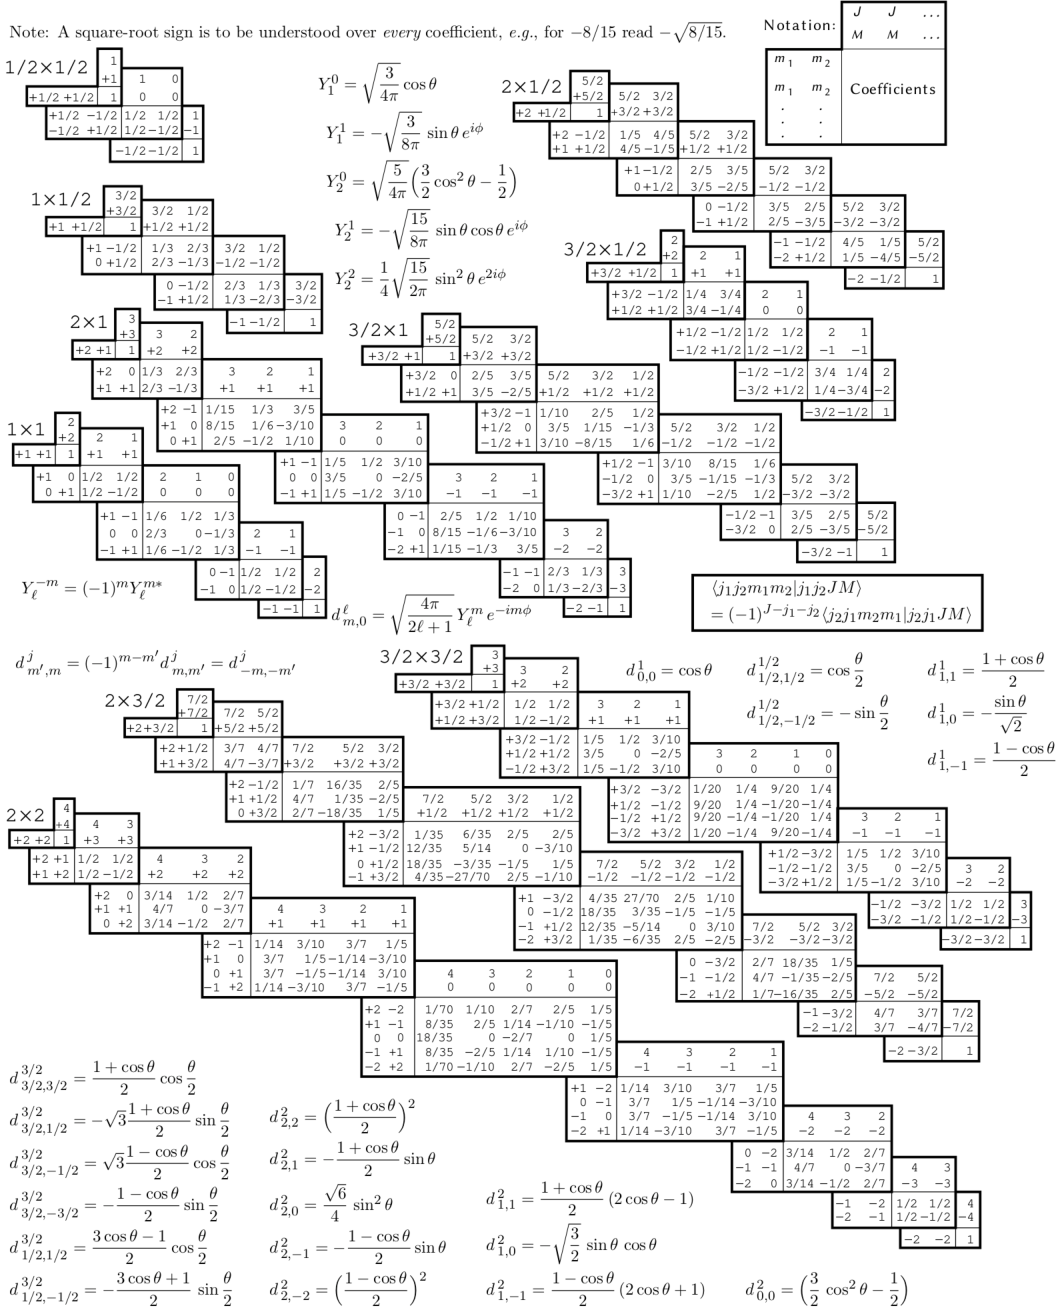
\includegraphics[width=\textwidth,height=\textheight]{clebschgordan1.pdf}
	\chapter{Tensor Spherical Harmonics}\label{app:tsh}
	In this appendix, we will treat the particular theme of spin-orbit angular momenta addition, and tensor spherical harmonics.\\
	We define our total angular momentum as follows
	\begin{equation}
		\vecopr{J}=\vecopr{L}\otimes\1+\1\otimes\vecopr{S}
		\label{eq:totalsoangmom}
	\end{equation}
	We then define our common basis between these operators and their projections, as in the general rules of angular momenta addition, using Clebsch-Gordan coefficients
	\begin{equation*}
		\ket{lsjm}=\sum_{m_l=-l}^l\sum_{m_s=-s}^s\bra{lsm_lm_s}\ket{lsjm}\ket{lsm_lm_s}
	\end{equation*}
By definition we then have that the eigenvalues of $\opr{J}^2,\opr{J}_z$ can then take the following values
	\begin{equation*}
		\begin{aligned}
			\abs{l-s}&\le j\le l+s\\
			m&=m_l+m_s
		\end{aligned}
	\end{equation*}
	We then recall that, in Schrödinger representation, the eigenfunctions of $\vecopr{L}$ and $\vecopr{S}$ are the following
	\begin{equation}
		\begin{dcases}
			\bra{x_i}\opr{S}^2\ket{sm_s}=\hbar^2s(s+1)\bra{x_i}\ket{sm_s}&\bra{x_i}\opr{S}_z\ket{sm_s}=\hbar m_s\bra{x_i}\ket{sm_s}\\
			\bra{x_i}\opr{L}^2\ket{lm_l}=\hbar^2l(l+1)\bra{x_i}\ket{lm_l}&\bra{x_i}\opr{L}_z\ket{lm_l}=\hbar m_l\bra{x_i}\ket{lm_l}
		\end{dcases}
		\label{eq:lseigen}
	\end{equation}
	Where $\bra{x_i}\ket{sm_s}=\chi_{sm_s}$ is the basis spinor and $\bra{x_i}\ket{lm_l}=Y^{m_l}_l(\theta,\phi)$ are the spherical harmonics.\\
	In the new basis of common eigenvectors of $\opr{J}^2,\opr{J}_z,\opr{L}^2,\opr{S}^2$ we then define the \textit{tensor spherical harmonics} $\bra{x_i}\ket{lsjm}=\mc{Y}^{ls}_{jm}(\theta,\phi)$ as follows
	\begin{equation}
		\begin{dcases}
			\opr{J}^2\mc{Y}^{ls}_{jm}(\theta,\phi)=\hbar^2j(j+1)\mc{Y}^{ls}_{jm}(\theta,\phi)&\opr{J}_z\tsph=\hbar m\tsph\\
			\opr{L}^2\tsph=\hbar^2l(l+1)\tsph&\opr{S}^2\tsph=\hbar^2s(s+1)\tsph
		\end{dcases}
		\label{eq:tsphaction}
	\end{equation}
	By definition then, we can define the tensor spherical harmonics as follows
	\begin{equation}
		\begin{aligned}
			\ket{lsjm}&=\sum_{m_l=-l}^l\sum_{m_s=-s}^s\bra{lsm_lm_s}\ket{jm}\ket{lm_l}\otimes\ket{sm_s}\\
			\tsph&=\sum_{m_l=-l}^l\sum_{m_s=-s}^s\bra{lsm_lm_s}\ket{jm}\bra{x_i}\ket{lm_l}\otimes\bra{x_i}\ket{sm_s}
		\end{aligned}
		\label{eq:tsphdef}
	\end{equation}
	Or, indicating the Clebsch-Gordan coefficients as $C^{lsm_lm_s}_{jm}$
	\begin{equation*}
		\tsph=C^{lsm_lm_s}_{jm}\sph\chi_{sm_s}
	\end{equation*}
	\section{Spin $1/2$ System}
	The overall problem simplifies enormously for $s=\frac{1}{2}$ systems. The permitted values of $j$ are $l+1/2$ and $l-1/2$ and, the Clebsch-Gordan coefficients, are then simply the following
	\begin{table}[H]
		\centering
		\begin{tabular}{|c|c|c|}
			\hline
			&&\\
			$j$&$m_s=\tfrac{1}{2}$&$m_s=-\tfrac{1}{2}$\\
			&&\\
			\hline
			&&\\
			$l+\frac{1}{2}$&$\sqrt{\frac{l+m+\frac{1}{2}}{2l+1}}$&$\sqrt{\frac{l+m+\frac{1}{2}}{2l+1}}$\\
			&&\\
			\hline
			&&\\
			$l-\frac{1}{2}$&$-\sqrt{\frac{l+m+\frac{1}{2}}{2l+1}}$&$\sqrt{\frac{l+m+\frac{1}{2}}{2l+1}}$\\
			&&\\
			\hline
		\end{tabular}
	\end{table}
	\begin{equation}
		\mc{Y}^{l\frac{1}{2}}_{l\pm\frac{1}{2},m}(\theta,\phi)=\frac{1}{\sqrt{2l+1}}\begin{pmatrix}\pm\sqrt{l\pm m+\tfrac{1}{2}}Y_l^{m-\frac{1}{2}}(\theta,\phi)\\\sqrt{l\mp m+\tfrac{1}{2}}Y^{m+\frac{1}{2}}_l(\theta,\phi)\end{pmatrix}
		\label{eq:tensorsphericalharm}
	\end{equation}
	Which can then be manipulated in order to get various useful informations, as spin-orbit coupling eigenvalues, which appear in atomic physics in the relativistic approximation of hydrogenoid atoms.
	\chapter{Calculation of $\expval{r^k}_{nlm}$ Integrals}\label{app:E}
	We know already that the wavefunction for a Hydrogen atom (non-normalized) is
	\begin{equation}
		\psi_{nlm}(x_i)=R_{nl}(r)Y^m_l(\theta,\phi)
		\label{eq:hydrogenwavefunctionappendix}
	\end{equation}
	Setting $a_0=\frac{4\hbar^2\pi\epsilon_0}{me^2}$ as our Bohr radius, we get that $R_{nl}$ for $1s,2s,2p$ states are
	\begin{equation}
		\begin{aligned}
			R_{10}&=2\left( \frac{a_0}{Z} \right)^{-\frac{3}{2}}e^{-\frac{Zr}{a_0}}\\
			R_{20}&=2\left( \frac{2a_0}{Z} \right)^{-\frac{3}{2}}\left( 1-\frac{Zr}{2a_0} \right)e^{-\frac{Zr}{2a_0}}\\
			R_{21}&=\sqrt{\frac{1}{3}}\frac{Zr}{a_0}\left( \frac{2a_0}{Z} \right)^{-\frac{3}{2}}e^{-\frac{Zr}{2a_0}}
		\end{aligned}
		\label{eq:rnlappendix}
	\end{equation}
	Hence, polynomials times an exponential with $r/a_0$ as a variable. The integral we have to calculate will then be
	\begin{equation}
		\expval{r^d}_{nlm}=\int_{0}^{\infty}r^{d+2}\abs{R_{nl}(r)}^2\diff{r}
		\label{eq:completeintegralrdapp}
	\end{equation}
	Which are of the kind
	\begin{equation}
		I(k,p)=\int_{0}^{\infty}r^ke^{-\frac{Zpr}{a_0}}\diff{r}
		\label{eq:integralstocalculate}
	\end{equation}
	Where $k,p\in\mathbb{N}$. Using a coordinate transformation $z=Zpr/a_0$ we have that the integral reduces to a Euler Gamma integral for whole numbers
	\begin{equation}
		I(k,p)=\left( \frac{a_0}{Zp} \right)^{k+1}\int_{0}^{\infty}z^ke^{-z}\diff{z}=\left( \frac{a_0}{Zp} \right)^{k+1}k!
		\label{eq:integralssolved}
	\end{equation}
	With this in mind, we calculate the especially useful expectation values for $r^{-i}$, with $i=1,2,3$ on $1s,2s,2p$ states of the Hydrogen atom, for which $Z=1$. These expectation values pop up when evaluating relativistic corrections for atoms.
	\begin{equation}
		\begin{aligned}
			\expval{\frac{1}{r}}_{1s}&=\frac{1}{a_0}\\
			\expval{\frac{1}{r}}_{2s}&=\frac{1}{2a_0^3}\left( I(1,1)-\frac{1}{a_0}I(2,1)+\frac{1}{4a_0^2}I(3,1) \right)=\frac{1}{4a_0}\\
			\expval{\frac{1}{r}}_{2p}&=\frac{1}{24a_0^5}I(3,1)=\frac{1}{4a_0}
		\end{aligned}
		\label{eq:rminusoneapp}
	\end{equation}
	Lowering $k$ by one we obtain the expectation values for $r^{-2}$
	\begin{equation}
		\begin{aligned}
			\expval{\frac{1}{r^2}}_{1s}&=\frac{2}{a_0}\\
			\expval{\frac{1}{r^2}}_{2s}&=\frac{1}{2a_0^3}\left( I(0,1)-\frac{1}{a_0}I(1,1)+\frac{1}{4a_0}I(2,1) \right)=\frac{1}{4a_0^2}\\
			\expval{\frac{1}{r^2}}_{2p}&=\frac{1}{24a_0^5}I(2,1)=\frac{1}{12a_0^2}
		\end{aligned}
		\label{eq:rminustwoapp}
	\end{equation}
	For $r^{-3}$ we will evaluate only the level $2p$, since this expectation value pops up with spin orbit interaction, which is null for $ns$ states
	\begin{equation}
		\expval{\frac{1}{r^3}}_{2p}=\frac{1}{24a_0^5}I(1,1)=\frac{1}{24a_0^3}
		\label{eq:rminusthreeapp}
	\end{equation}
	\chapter{Periodic Table}
	\vfill
	\newpage
	\begin{figure}[H]
		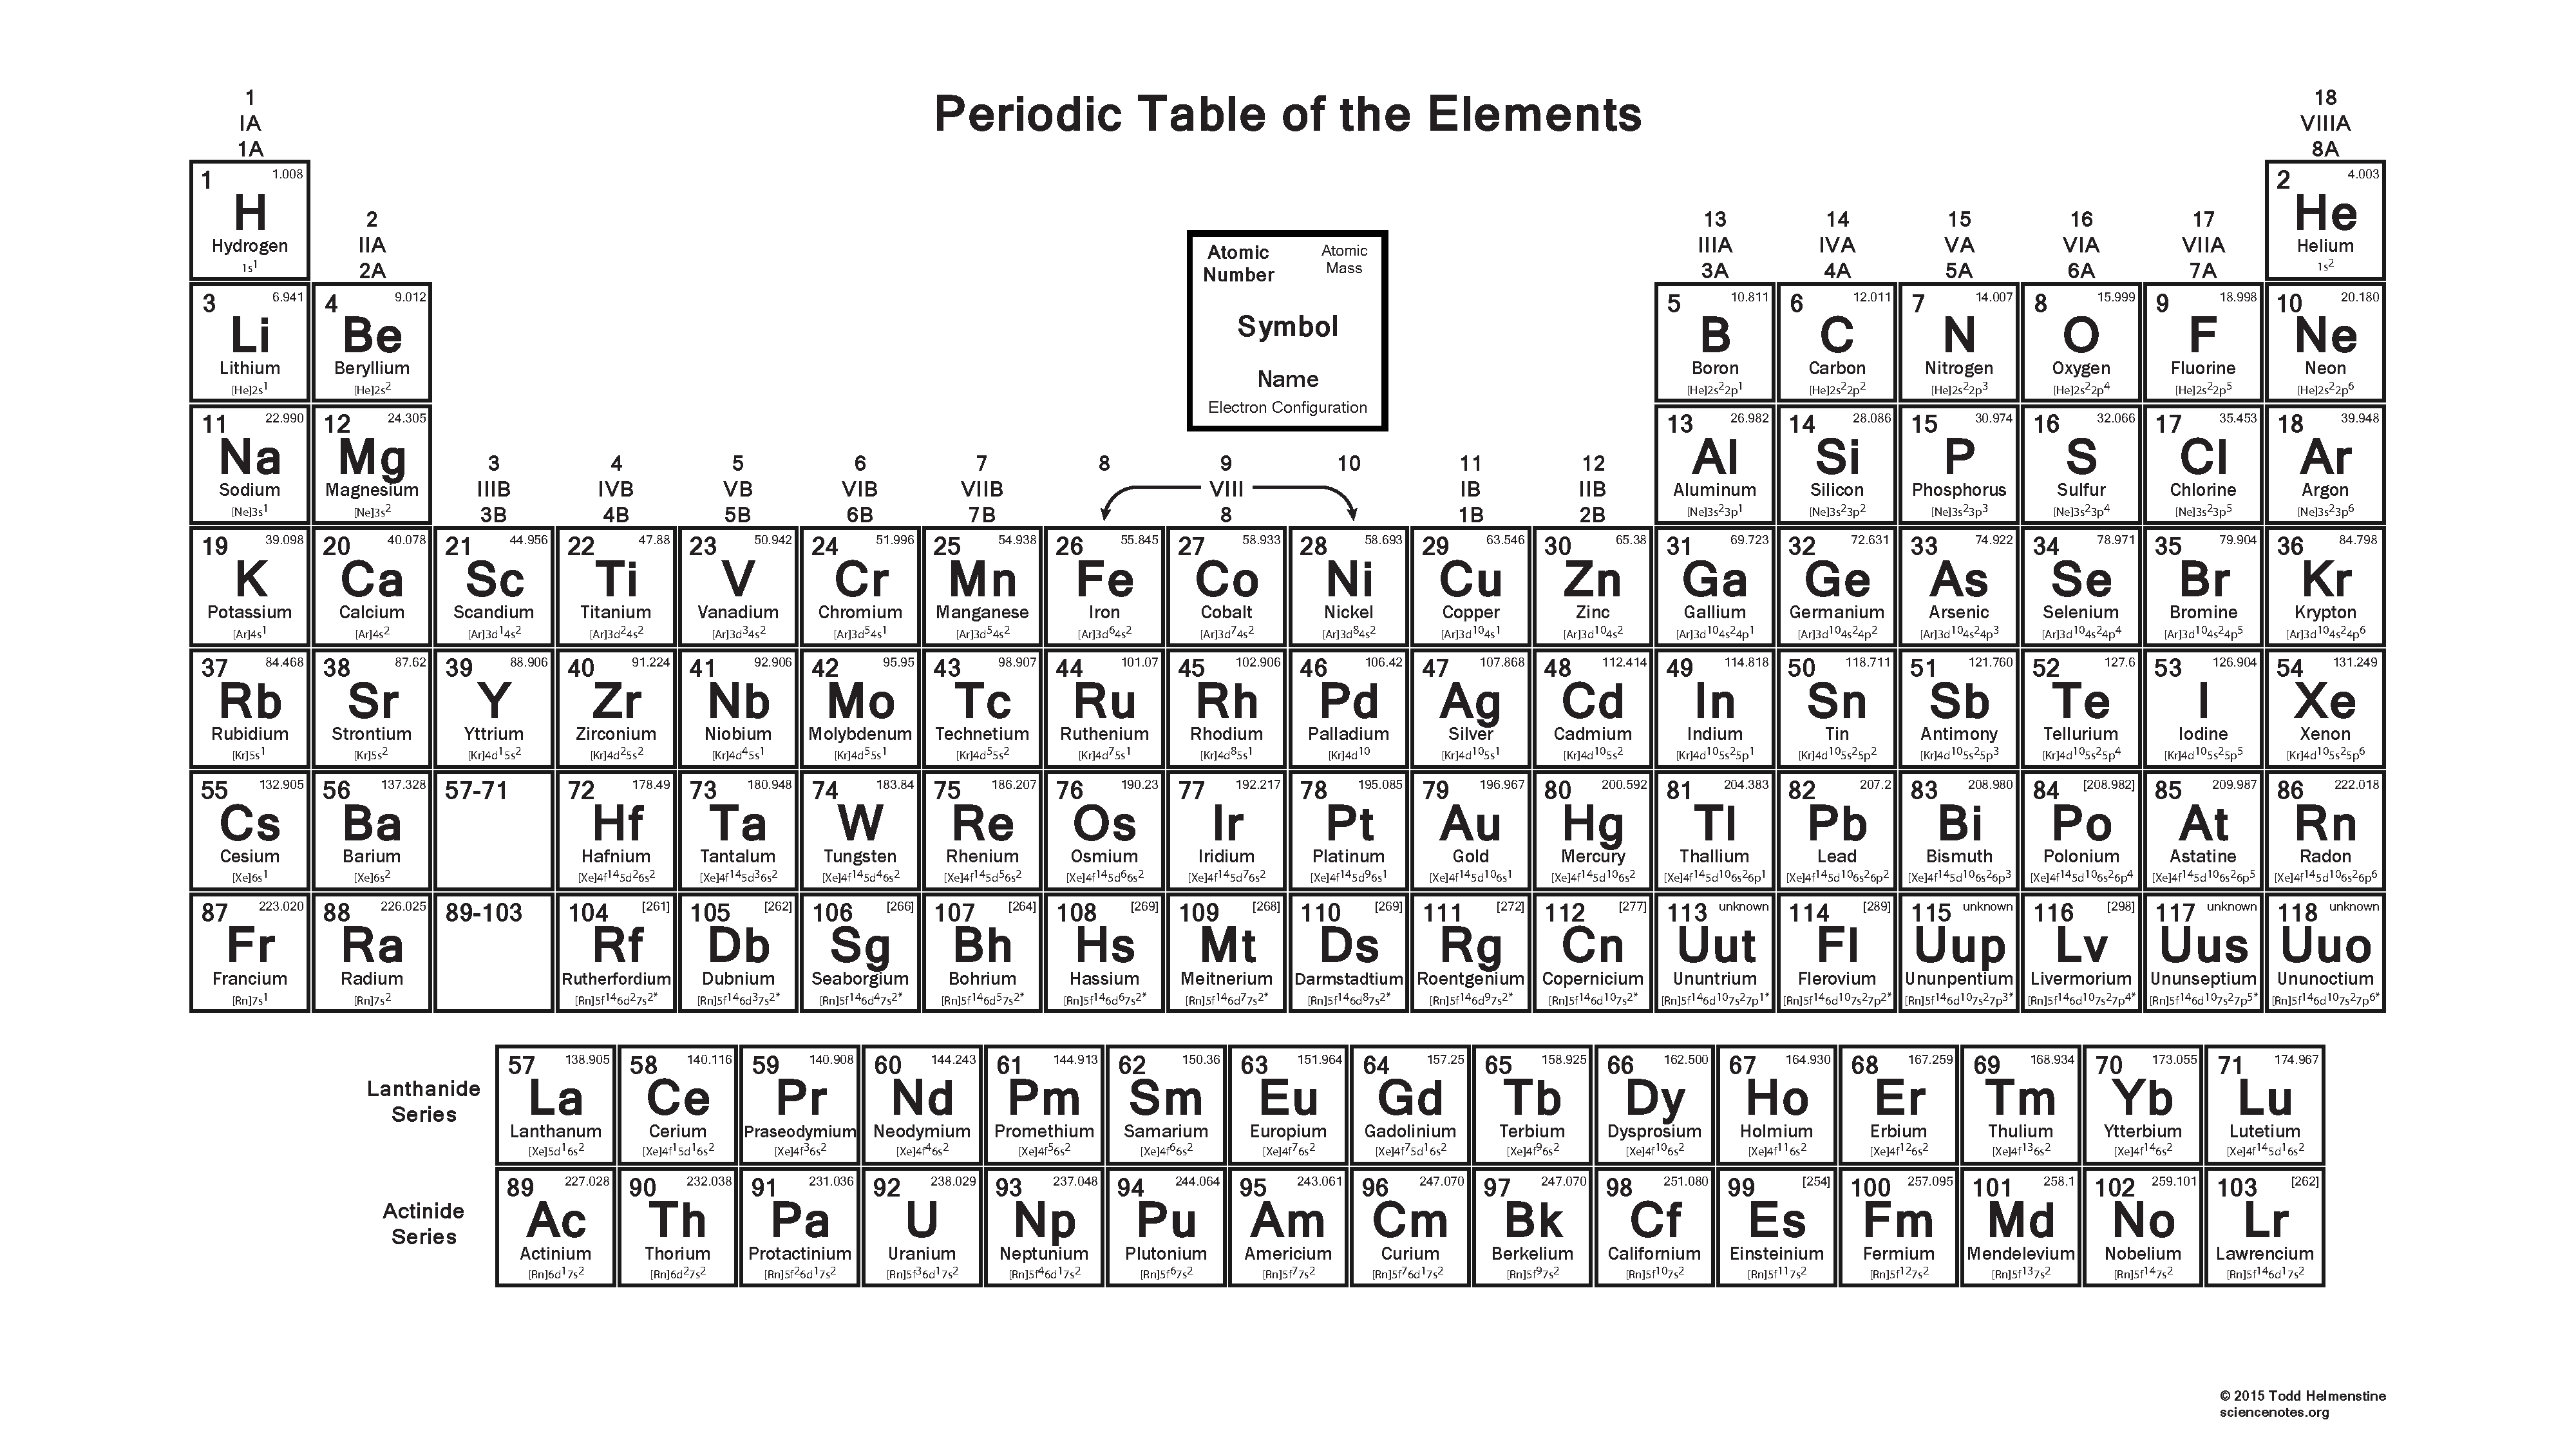
\includegraphics[angle=90, width=\linewidth]{ptwconf.pdf}
	\end{figure}
	\chapter{Symmetry and Groups}\label{app:groups}
	We can categorize symmetry transformations in various ways, but principally, we have 3 fundamental transformations
	\begin{enumerate}
	\item Rotations through an axis
	\item Reflections on a plane
	\item Parallel displacements
	\end{enumerate}
	It's obvious that the last kind of transformation, in our field, will have sense only in infinite mediums like lattices and solids, hence, for molecules, we'll be interested principally in the first two: \textit{rotations} and \textit{reflections}.\\
	Let's start by defining a rotation operator $\opr{C}_n$, where $n\in\N$. The whole number $n$ is called \textit{order of symmetry} of the considered axis, which means that the system will be again in the initial transformation after $n$ rotations of $\alpha=2\pi/n$ degrees.\\
	We can immediately determine two fundamental properties of the rotation operator from this
	\begin{equation*}
		\begin{aligned}
			\opr{C}_1&=1\\
			\opr{C}_n^n&=\1
		\end{aligned}
	\end{equation*}
	The second operator we will define, is the plane reflection operator $\opr{\sigma}$, which operates through a reflection of the system on a predetermined plane, and finally we can define the inversion operator $\opr{I}$, which corresponds to a complete inversion of the coordinate system used.\\
	\section{Group Theory}
	In order to delve deeper into the theory of symmetry, we need to define what a group is mathematically and how does it work, since symmetries of the system arise from the invariance of the Hamiltonian to transformations pertaining to one of these groups.\\
	So let's begin by calling the set $G$ a group. In order to be such, it has to have the following properties
	\begin{enumerate}
	\item Identity: $\1\in G$
	\item Associativity: $(\opr{a}\opr{b})\opr{c}=\opr{a}(\opr{b}\opr{c})\ \forall\opr{a},\opr{b},\opr{c}\in G$
	\item Non Commutativity: $\opr{a}\opr{b}\ne\opr{b}\opr{a}\ \forall\opr{a},\opr{b}\in G$
	\item Existence of the inverse: $\forall\opr{a}\in G\ \exists!\opr{a}^{-1}\in G:\opr{a}^{-1}\opr{a}=\1=\opr{a}\opr{a}^{-1}$
	\item $\forall\opr{a},\opr{b}\in G\ (\opr{a}\opr{b})^{-1}=\opr{b}^{-1}\opr{a}^{-1}$
	\end{enumerate}
	A group is said abelian, if and only if $\forall\opr{a}\opr{b}\in G,\ \opr{a}\opr{b}=\opr{b}\opr{a}$, hence it's \textit{commutative}.\\
	From an abelian group, one can define a cyclic group, which is an abelian group for which $\forall\opr{a}\in G,\exists n\in\N:\ \opr{a}^n=\1$. The integer $n$ is called the \textit{order} of the group $G$, and it's usually indicated as $\{G\}$.\\
	\begin{defn}[Finite Group]
		A finite group is a group $G$ for which there exists a finite number of elements.
	\end{defn}
	\begin{defn}[Subgroup]
		A subset $H\subset G$ is a subgroup, if and only if has all the properties of a group.
	\end{defn}
	\begin{defn}[Complex]
		Let $H\subset G$ be a subgroup of a finite group (hence, a finite subgroup). Since $H\subset G$, there exists a finite number of elements $G_i\in G$, for which $G_i\notin H$. We can then define a new element of $G$ which is not an element of $H$ by multiplying all elements of $H$ with a single $G_i$.\\
		The new algebraic construction is called \textit{complex}.\\
		In general, if $G$ is a group, and $L,H\subset G$ are subgroups of $G$, for which $L=G\setminus H$, $\forall \opr{l}_i\in L,\ \opr{h}\in H$, the product $\opr{h}\opr{l}_i$ generates another $n$ subgroups of $G$ called \textit{complexes}.\\
		Since these all are finite groups by hypothesis, if $\{L\}=l,\ \{H\}=h$, then $\{G\}=\{H\}\{L\}$.
	\end{defn}
	\begin{defn}[Direct Product]
		A direct product of two groups $A,B$, indicated as $A\otimes B$, is defined as follows
		\begin{equation*}
			A\otimes B:=\left\{ \opr{a}\in A, \opr{b}\in B:\ \opr{a}\opr{b}\in A\otimes B \right\}
		\end{equation*}
	\end{defn}
	We can now start talking about \textit{molecular point groups}. We start by defining rotation groups.\\
	\textbf{$C_n$ group}\\
	The group $C_n$ is the group of symmetries around a rotation axis of the $n$-th order.\\\vskip\baselineskip
	\textbf{$S_{2n}$ group}\\
	The $S_{2n}$ group is the \textit{rotoreflection} group of a single axis of the $n$-th order. Two special cases of this group are the $S_2$ and $S_{4p+2}$ group, which are
	\begin{equation*}
		\begin{aligned}
			S_2:&=\{\1,\opr{I}\}=C_i\\
			S_{4p+2}&=C_{2p+1}\otimes C_i
		\end{aligned}
	\end{equation*}\\\vskip\baselineskip
	\textbf{$C_{nh}$ group}\\
	The $C_{nh}$ group is the group of simmetries around an axis of the $n$-th order, coupled with a symmetry through a plane perpendicular to the axis. This group can be seen as a complex created from $n$ $\opr{C}_{n}$ elements and one $\opr{\sigma}_h$ element as follows. It's also obvious that it's Abelian
	\begin{equation*}
		\opr{C}_{nh}=\opr{C}_n^k\otimes\opr{\sigma}_h=\opr{\sigma}_h\otimes\opr{C}_n^k
	\end{equation*}
	A special case is the group $C_{1h}$, which is formed by two elements
	\begin{equation*}
		C_{1h}:=\{\1,\opr{\sigma}_h\}=C_s
	\end{equation*}\\\vskip\baselineskip
	\textbf{$C_{nv}$ group}\\
	The $C_{nv}$ group is similar to the $C_{nh}$ group, but the $n$-th order symmetry axis lies on the symmetry plane. This generates $n-1$ more planes of symmetry separated by an angle $\alpha=\pi/n$\\\vskip\baselineskip
	\textbf{$D_n$ group}\\
	The $D_n$ group is formed from a symmetry axis of order $n$, which is perpendicular to an axis of order 2. I.e. it's formed from an axis of order $n$ and $n-1$ axes of order 2 separated from an angle $\alpha=\pi/n$. A special case is given by the group $D_2=V$, which is formed from an two axes of order 2 perpendicular to each other\\\vskip\baselineskip
	\textbf{$D_{nh}$ group}\\
	The $D_{nh}$ group is a complex formed from the product $D_n\otimes C_s$, i.e. for every order $2$ axis there lies a plane perpendicular to such axis.\\\vskip\baselineskip
	\textbf{$D_{nd}$ group}\\
	Starting from the $D_{nh}$ group, one can define the group $D_{nd}$ by taking the planes at a separation of $\alpha=\pi/2n$ radians.\\\vskip\baselineskip
	\textbf{$T$ group}\\
	The $T$ group is the group formed from the symmetries of the tetrahedron. This group can be formed from the group $V$ ($D_2$), coupled with 4 oblique $C_3$ axes.\\\vskip\baselineskip
	\textbf{$T_d$ group}\\
	The $T_d$ group is formed from the $T$ group by adding a plane of symmetry to the tetrahedron, it's formally given by the product $T_d=T\otimes C_s$\\\vskip\baselineskip
	\textbf{$T_h$ group}\\
	The $T_h$ group, instead is formed from the $T$ group through addition of a center of symmetry, i.e. a point of inversion. This is described by the product $T_h=T\otimes C_i$\\\vskip\baselineskip
	\textbf{$O$ group}\\
	The $O$ group is the group given by the symmetries of the octahedron. Adding a center of symmetry, we obtain the group $O_h=O\otimes C_i$.
	\nocite{quantistica,landau3,statistica,struttura,struttura1,griffmq,sakuraimqm,patritesta,molekulphysik,complessa}
%	\listoftables
%	\listoffigures
	\printbibliography
\end{document}
